%\documentclass[aps,prb,onecolumn,nofootinbib]{revtex4}  
\documentclass[12pt,a4paper]{article}
\usepackage[margin=1in]{geometry}  % set the margins to 1in on all sides
%\usepackage{jheppub}
\usepackage{amsmath,amsfonts,amssymb,latexsym,dsfont}
\usepackage{hhline}
\usepackage{graphicx}
%\usepackage[arrow,matrix]{xy}
\usepackage[all]{xy}
\usepackage{tikz}
\usepackage{tikz-cd}
\definecolor{hanpurple}{rgb}{0.32, 0.09, 0.98}
\setcounter{MaxMatrixCols}{12}
\usepackage{tabu}

\usepackage[numbers]{natbib}
\usepackage[colorlinks]{hyperref}
\hypersetup{linkcolor={hanpurple}}



\usetikzlibrary{positioning,arrows}
\usetikzlibrary{decorations.pathmorphing}
\usetikzlibrary{decorations.markings}

\usetikzlibrary{decorations.pathreplacing,calc}

\newcommand{\tikzmark}[2][-3pt]{\tikz[remember picture, overlay, baseline=-0.5ex]\node[#1](#2){};}

\tikzset{brace/.style={decorate, decoration={brace}},
 brace mirrored/.style={decorate, decoration={brace,mirror}},
}

\newcounter{brace}
\setcounter{brace}{0}
\newcommand{\drawbrace}[3][brace]{%
 \refstepcounter{brace}
 \tikz[remember picture, overlay]\draw[#1] (#2.center)--(#3.center)node[pos=0.5, name=brace-\thebrace]{};
}

\newcounter{arrow}
\setcounter{arrow}{0}
\newcommand{\drawcurvedarrow}[3][]{%
 \refstepcounter{arrow}
 \tikz[remember picture, overlay]\draw (#2.center)edge[#1]node[coordinate,pos=0.5, name=arrow-\thearrow]{}(#3.center);
}

% #1 options, #2 position, #3 text 
\newcommand{\annote}[3][]{%
 \tikz[remember picture, overlay]\node[#1] at (#2) {#3};
}

\newcommand{\tp}{\otimes}
\newcommand{\tpc}{\tilde{\otimes}}
\newcommand{\ra}{\rightarrow}
\newcommand{\unit}{\mathds{1}}
\newcommand{\zz}{\mathbb{Z}}
\newcommand{\mce}{\mathcal{E}}
\newcommand{\cc}{\mathbb{C}}
\newcommand{\rr}{\mathbb{R}}
\newcommand{\mcr}{\mathcal{R}}
\newcommand{\mcz}{\mathcal{Z}}
\newcommand{\mca}{\mathcal{A}}
\newcommand{\mcd}{\mathcal{D}}
\newcommand{\mcg}{\mathcal{G}}
\newcommand{\mct}{\mathcal{T}}
\newcommand{\mcs}{\mathcal{S}}
\newcommand{\ul}{\underline}
\newcommand{\Mod}{\text{Mod}}
\newcommand{\Aut}{\text{Aut}}
\newcommand{\ulmcc}{\underline{\mathcal{C}}}
\newcommand{\zt}{\mathbb{Z}_2}
\newcommand{\oeo}{\text{others = 1}}
\newcommand\be            {\begin{equation}}
\newcommand\ee            {\end{equation}}
\newcommand\ba            {\begin{aligned}}
\newcommand\ea            {\end{aligned}}
\newcommand{\mcf}{\mathcal{F}}
\newcommand{\spinz}{\text{\sffamily{Z}}}
\newcommand{\spinx}{\text{\sffamily{X}}}
\newcommand{\mcl}{\mathcal{L}}
\newcommand{\mcc}{\mathcal{C}}
\newcommand{\mco}{\mathcal{O}}
\newcommand{\mcm}{\mathcal{M}}
\newcommand{\zc}{\mathcal{Z}(\mathcal{C})}
\newcommand{\id}{\text{id}}
\newcommand{\Hom}{\text{Hom}}
\newcommand{\End}{\text{End}}
\newcommand{\Tor}{\text{Tor}}
\newcommand{\Ext}{\text{Ext}}
\newcommand{\p}{\partial}
\newcommand{\wt}{\widetilde}
\usepackage{verbatim}
\newcommand{\cl}{\mathbb{C}\ell}
\newcommand{\vect}{\text{Vec}}
\newcommand{\svect}{\text{sVec}}
\newcommand{\spin}{\text{Spin}}
\newcommand{\pin}{\text{Pin}}
\newcommand{\fube}{\textbf{Tube}}
\newcommand{\tube}{\textbf{Tube}}
\newcommand{\fld}{\mathcal{F}} %fld was for field config

% KW
\newcommand{\ot}{\otimes}
\newcommand{\bd}{\partial}
\DeclareMathOperator{\Arf}{Arf}

\newcommand{\bra}[1]{\ensuremath{\left\langle#1\right|}}
\newcommand{\ket}[1]{\ensuremath{\left|#1\right\rangle}}

\definecolor{ao(english)}{rgb}{0.0, 0.5, 0.0}
\definecolor{americanrose}{rgb}{1.0, 0.01, 0.24}
\definecolor{amber(sae/ece)}{rgb}{1.0, 0.49, 0.0}

\newcommand{\dave}[1]{{\color{ao(english)}\footnotesize{(DA) #1}}}
\newcommand{\remove}[1]{{\color{amber(sae/ece)}\footnotesize{(RM?) #1}}}

%a purple that looks different from red. EL: nice! I like the name
\definecolor{amethyst}{rgb}{0.6, 0.4, 0.8}
\newcommand{\ethan}[1]{{\color{amethyst}\footnotesize{(EL) #1}}}

\definecolor{kwcolor}{rgb}{0.2, 0.5, 0.85}
\newcommand{\kw}[1]{{\color{kwcolor}\footnotesize{(KW) #1}}}
\newcommand{\kwsep}{\bigskip\hrule\medskip\hrule\medskip\hrule\bigskip}

\newcommand{\abullet}{{\color{amethyst} \bullet}}

\newcommand{\CapDotLeft}{\mathord{\vcenter{\hbox{
\includegraphics[scale=1]{CapDotLeft.pdf}}}}}
\newcommand{\CapDotRight}{\mathord{\vcenter{\hbox{
\includegraphics[scale=1]{CapDotRight.pdf}}}}}
\newcommand{\CupDotLeft}{\mathord{\vcenter{\hbox{
\includegraphics[scale=1,angle=180,origin=c]{CapDotRight.pdf}}}}}
\newcommand{\CupDotRight}{\mathord{\vcenter{\hbox{
\includegraphics[scale=1,angle=180,origin=c]{CapDotLeft.pdf}}}}}

\newcommand{\CupCapPsi}{\mathord{\vcenter{\hbox{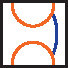
\includegraphics[scale=1]{cupcappsi.pdf}}}}}

\newcommand{\Qcap}{\mathord{\vcenter{\hbox{
\includegraphics[scale=1]{Qcap.pdf}}}}}
\newcommand{\Qcup}{\mathord{\vcenter{\hbox{
\includegraphics[scale=1,angle=180,origin=c]{Qcap.pdf}}}}}
\newcommand{\Qdotdot}{\mathord{\vcenter{\hbox{
\includegraphics[scale=1]{Qdotdot.pdf}}}}}
\newcommand{\QIdentity}{\mathord{\vcenter{\hbox{
\includegraphics[scale=1]{QIdentity.pdf}}}}}

\newcommand{\CupCap}{\mathord{\vcenter{\hbox{
\includegraphics[scale=1]{CupCap.pdf}}}}}
\newcommand{\CupCapDots}{\mathord{\vcenter{\hbox{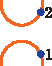
\includegraphics[scale=1]{CupCapDots.pdf}}}}}

\newcommand{\SigmaDotDot}{\mathord{\vcenter{\hbox{
\includegraphics[scale=1]{SigmaDotDot.pdf}}}}}
\newcommand{\SigmaDotDotExchange}{\mathord{\vcenter{\hbox{
\includegraphics[scale=1]{SigmaDotDotExchange.pdf}}}}}
\newcommand{\TwoLine}{\mathord{\vcenter{\hbox{
\includegraphics[scale=1]{TwoLine.pdf}}}}}
\newcommand{\TwoLineDots}{\mathord{\vcenter{\hbox{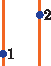
\includegraphics[scale=1]{TwoLineDots.pdf}}}}}

\newcommand{\RDotTwo}{\mathord{\vcenter{\hbox{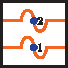
\includegraphics[scale=1]{RDotTwo.pdf}}}}}
\newcommand{\RDotTwoa}{\mathord{\vcenter{\hbox{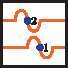
\includegraphics[scale=1]{RDotTwoa.pdf}}}}}
\newcommand{\RDotTwob}{\mathord{\vcenter{\hbox{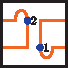
\includegraphics[scale=1]{RDotTwob.pdf}}}}}
\newcommand{\RDotTwoc}{\mathord{\vcenter{\hbox{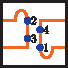
\includegraphics[scale=1]{RDotTwoc.pdf}}}}}

\newcommand{\FubeXXX}{\mathord{\vcenter{\hbox{
\includegraphics[scale=1]{EmptyTube.pdf}}}}}
\newcommand{\FubeXss}{\mathord{\vcenter{\hbox{
\includegraphics[scale=1]{OneLine.pdf}}}}}
\newcommand{\FubeXsds}{\mathord{\vcenter{\hbox{
\includegraphics[scale=1]{OneLineDot.pdf}}}}}



\newcommand{\AnnulusBare}{\mathord{\vcenter{\hbox{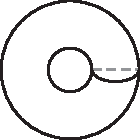
\includegraphics[scale=.6]{AnnulusBare.pdf}}}}}
\newcommand{\AnnularTube}{\mathord{\vcenter{\hbox{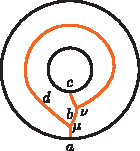
\includegraphics[scale=1]{AnnularTube.pdf}}}}}
\newcommand{\AnnularTubeNoIndex}{\mathord{\vcenter{\hbox{
\includegraphics[scale=1]{AnnularTubeNoIndex.pdf}}}}}
\newcommand{\AnnulusTubeTube}{\mathord{\vcenter{\hbox{
\includegraphics[scale=1]{AnnulusTubeTube.pdf}}}}}

\newcommand{\SAnnulusNoLabel}{\mathord{\vcenter{\hbox{
\includegraphics[scale=1]{SAnnulusNoLabel.pdf}}}}}
\newcommand{\TAnnulusNoLabel}{\mathord{\vcenter{\hbox{
\includegraphics[scale=1]{TAnnulusNoLabel.pdf}}}}}



\newcommand{\AnnulsLabel}[5]{\mathord{ 
\mkern2mu\overset{#3}{{\Annulusxprime{#1}{#2}}}\mkern2mu\raisebox{0ex}{$\scriptstyle{#4}$} }}

\newcommand*{\Annulus}[2]{{ #1 }
\kern-3.5em\raisebox{1ex}{ $\scriptstyle{#2}$} \kern2.6em} %Could change 0 to 1.2 to raise the B.

\newcommand*{\AnnulusP}[3]{{{\Annulus{#1}{#2}} }
\kern-.5em\raisebox{3.5ex}{ $\scriptstyle{#3}$} \kern.3em} %Could change 0 to 1.2 to raise the B.

\newcommand*{\AnnulusPx}[4]{\AnnulusP{#1}{#2}{#3}
\kern-3.6em\raisebox{-4.5ex}{ $\scriptstyle{#4}$} \kern2.6em} %Could change 0 to 1.2 to raise the B.

\newcommand*{\AnularTubex}[6]{\AnnulusPx{#1}{#2}{#3}{#4}
\kern-4em\raisebox{-4.5ex}{ $\overset{#6}{\underset{#5}{\vphantom{\Big|^2}}}$} \kern3em} %Could change 0 to 1.2 to raise the B.

\newcommand*{\TorusTubex}[6]{\AnnulusPx{#1}{#2}{#3}{#4}
\kern-4em\raisebox{-4.5ex}{ $\overset{#6}{\underset{#5}{\vphantom{\Big|^2}}}$} \kern3em} %Could change 0 to 1.2 to raise the B.

%\newcommand*{\AnnularTubex}[5]{\AnnulusPx{#1}{#2}{}{\; \; \;#3}
%\kern-3.9em\raisebox{-4.5ex}{ $\overset{#5}{\underset{#4}{\vphantom{\Big|^2}}}$} \kern2.7em} %Could change 0 to 1.2 to raise the B.



\newcommand{\SAnnulusx}[3]{\mathrel{\ooalign{$\SAnnulusNoLabel$\cr
  \hidewidth\raise5ex\hbox{$\scriptstyle{#3}\mkern1mu$}\cr
  \hidewidth\raise.8ex\hbox{$\scriptstyle{#2}\mkern63mu$}\cr
    \hidewidth\raise-3.8ex\hbox{$\scriptstyle{#1}\mkern39mu$}\cr
  }}}
  
  \newcommand{\TAnnulusx}[3]{\mathrel{\ooalign{$\TAnnulusNoLabel$\cr
  \hidewidth\raise5ex\hbox{$\scriptstyle{#3}\mkern1mu$}\cr
  \hidewidth\raise.8ex\hbox{$\scriptstyle{#2}\mkern63mu$}\cr
    \hidewidth\raise-4.9ex\hbox{$\scriptstyle{#1}\mkern51mu$}\cr
  }}}

\newcommand{\AnnularTubex}[6]{\mathrel{\ooalign{$#1$\cr
  \hidewidth\raise5ex\hbox{$\scriptstyle{#6}\mkern1mu$}\cr
  \hidewidth\raise.8ex\hbox{$\scriptstyle{#5}\mkern63mu$}\cr
  \hidewidth\raise-.9ex\hbox{$\scriptstyle{#3}\mkern68mu$}\cr
    \hidewidth\raise-4.5ex\hbox{$\scriptstyle{#4} \mkern50mu$}\cr
  \hidewidth\raise-7ex\hbox{$\scriptstyle{#2}\mkern68mu$}\cr
  }}}
  
%\newcommand{\AnnularTubexp}[9]{\mathrel{\ooalign{$#1$\cr
  %\hidewidth\raise5ex\hbox{$\scriptstyle{#9}\mkern1mu$}\cr
 %\hidewidth\raise.8ex\hbox{$\scriptstyle{#8}\mkern63mu$}\cr
 % \hidewidth\raise-3.4ex\hbox{$\scriptstyle{#7}\mkern68mu$}\cr
  %  \hidewidth\raise-5.1ex\hbox{$\scriptstyle{#6}\mkern80mu$}\cr
%  \hidewidth\raise-2.2ex\hbox{$\scriptstyle{#5}\mkern90mu$}\cr
 % \hidewidth\raise-.9ex\hbox{$\scriptstyle{#4}\mkern68mu$}\cr
%    \hidewidth\raise-4.5ex\hbox{$\scriptstyle{#3} \mkern50mu$}\cr
 % \hidewidth\raise-7ex\hbox{$\scriptstyle{#2}\mkern68mu$}\cr
 % }}}



\newcommand{\AnnularTubexp}[9]{\mathrel{\ooalign{$#1$\cr
  \hidewidth\raise5ex\hbox{$\scriptstyle{#9}\mkern1mu$}\cr
 \hidewidth\raise.8ex\hbox{$\scriptstyle{#8}\mkern63mu$}\cr
  \hidewidth\raise-3.7ex\hbox{$\scriptstyle{#7}\mkern50mu$}\cr
    \hidewidth\raise-5.1ex\hbox{$\scriptstyle{#6}\mkern57mu$}\cr
  \hidewidth\raise-2.2ex\hbox{$\scriptstyle{#5}\mkern90mu$}\cr
  \hidewidth\raise-.9ex\hbox{$\scriptstyle{#4}\mkern68mu$}\cr
    \hidewidth\raise-3.8ex\hbox{$\scriptstyle{#3} \mkern69mu$}\cr
  \hidewidth\raise-7ex\hbox{$\scriptstyle{#2}\mkern68mu$}\cr
  }}}


\newcommand{\SmallTorus}[3]{\mathrel{\ooalign{$#1$\cr
  \hidewidth\raise0ex\hbox{$\scriptstyle{#2}\mkern36mu$}\cr
    \hidewidth\raise-1.5ex\hbox{$\scriptstyle{#3}\mkern10mu$}\cr
  }}}
  
  
  \newcommand{\AnnulusTubeTubex}[6]{\mathrel{\ooalign{$#1$\cr
%  \hidewidth\raise5ex\hbox{$\scriptstyle{#7}\mkern1mu$}\cr
  \hidewidth\raise.8ex\hbox{$\scriptstyle{#6}\mkern65mu$}\cr
  \hidewidth\raise-.5ex\hbox{$\scriptstyle{#3}\mkern68mu$}\cr
    \hidewidth\raise-4.9ex\hbox{$\scriptstyle{#4} \mkern50mu$}\cr
     \hidewidth\raise-2.7ex\hbox{$\scriptstyle{#5} \mkern54mu$}\cr
  \hidewidth\raise-7.3ex\hbox{$\scriptstyle{#2}\mkern68mu$}\cr
  }}}
  


\newcommand{\TorusLocalRelationc}{\mathord{\vcenter{\hbox{
\includegraphics[scale=1]{TorusLocalRelationc.pdf}}}}}
\newcommand{\TorusLocalRelationb}{\mathord{\vcenter{\hbox{
\includegraphics[scale=1]{TorusLocalRelationb.pdf}}}}}
\newcommand{\TorusLocalRelationa}{\mathord{\vcenter{\hbox{
\includegraphics[scale=1]{TorusLocalRelationa.pdf}}}}}


\newcommand{\Dv}{\mathord{\vcenter{\hbox{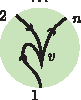
\includegraphics[scale=1]{Dv.pdf}}}}}
\newcommand{\Dfv}{\mathord{\vcenter{\hbox{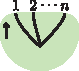
\includegraphics[scale=1]{Dfv.pdf}}}}}


\newcommand{\Horseshoe}{\mathord{\vcenter{\hbox{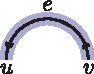
\includegraphics[scale=1]{Horseshoe.pdf}}}}}
\newcommand{\HorseshoeTwist}{\mathord{\vcenter{\hbox{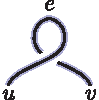
\includegraphics[scale=1]{HorseshoeTwist.pdf}}}}}
\newcommand{\euv}{\mathord{\vcenter{\hbox{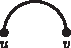
\includegraphics[scale=1]{euv.pdf}}}}}
\newcommand{\chieuv}{\mathord{\vcenter{\hbox{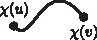
\includegraphics[scale=1]{chieuv.pdf}}}}}



\newcommand{\TaddownTubeNoLabel}{\mathord{\vcenter{\hbox{
\includegraphics[scale=1]{TaddownTube.pdf}}}}}
\newcommand{\TadupTubeNoLabel}{\mathord{\vcenter{\hbox{
\includegraphics[scale=1]{TadupTube.pdf}}}}}
\newcommand{\hTube}{\mathord{\vcenter{\hbox{
\includegraphics[scale=1]{hTube.pdf}}}}}
\newcommand{\tTube}{\mathord{\vcenter{\hbox{
\includegraphics[scale=1]{tTube.pdf}}}}}
\newcommand{\eTube}{\mathord{\vcenter{\hbox{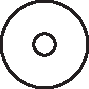
\includegraphics[scale=1]{eTube.pdf}}}}}
\newcommand{\vTube}{\mathord{\vcenter{\hbox{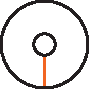
\includegraphics[scale=1]{vTube.pdf}}}}}


\newcommand{\dota}{\mathord{\vcenter{\hbox{
\includegraphics[scale=1]{dota.pdf}}}}}
\newcommand{\dotb}{\mathord{\vcenter{\hbox{
\includegraphics[scale=1]{dotb.pdf}}}}}
\newcommand{\dotc}{\mathord{\vcenter{\hbox{
\includegraphics[scale=1]{dotc.pdf}}}}}

\newcommand{\XTubeNoLabel}{\mathord{\vcenter{\hbox{
\includegraphics[scale=1]{XTube.pdf}}}}}
\newcommand{\XTube}[2]{\mathrel{\ooalign{$\XTubeNoLabel$\cr
  \hidewidth\raise-2.5ex\hbox{$\scriptstyle{#2}\mkern28mu$}\cr
    \hidewidth\raise-2.9ex\hbox{$\scriptstyle{#1}\mkern50mu$}\cr
  }}}


\newcommand{\TaddownTube}[1]{\mathrel{\ooalign{$\TaddownTubeNoLabel$\cr
    \hidewidth\raise-2.8ex\hbox{$\scriptstyle{#1}\mkern30mu$}\cr
  }}}
  \newcommand{\TadupTube}[1]{\mathrel{\ooalign{$\TadupTubeNoLabel$\cr
    \hidewidth\raise-2.6ex\hbox{$\scriptstyle{#1}\mkern30mu$}\cr
  }}}
  
  \newcommand{\TorusNoLabels}{\mathord{\vcenter{\hbox{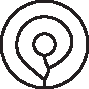
\includegraphics[scale=1]{TorusNoLabels.pdf}}}}}
\newcommand{\TorusNoLabelsx}[1]{\mathrel{\ooalign{$\TorusNoLabels$\cr
    \hidewidth\raise-2.8ex\hbox{$\scriptstyle{#1}\mkern30mu$}\cr
  }}}

\newcommand{\VerticalSpace}{\mathord{\vcenter{\hbox{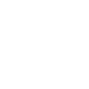
\includegraphics[scale=1]{VerticalSpace.pdf}}}}}

\newcommand{\AddDat}[3]{\mathrel{\ooalign{  $#1$\cr
  \hidewidth\raise0ex\hbox{$\scriptstyle{#2}\mkern38mu$}\cr
  \hidewidth\raise0ex\hbox{${#3}\mkern0mu$}\cr
  \hidewidth\raise0ex\hbox{$\VerticalSpace$}\cr
  }}}
  
  \newcommand{\AddDatTorus}[3]{\mathrel{\ooalign{  $#1$\cr
  \hidewidth\raise0ex\hbox{$\scriptstyle{#2}\mkern38mu$}\cr
  \hidewidth\raise3.8ex\hbox{$\scriptstyle{#3}\mkern0mu$}\cr
  \hidewidth\raise0ex\hbox{$\VerticalSpace$}\cr
  }}}
  
    \newcommand{\AddDatTorusDot}[4]{\mathrel{\ooalign{  $#1$\cr
  \hidewidth\raise0ex\hbox{$\scriptstyle{#2}\mkern38mu$}\cr
  \hidewidth\raise3.8ex\hbox{$\scriptstyle{#3}\mkern0mu$}\cr
  \hidewidth\raise0ex\hbox{${#4}\mkern0mu$}\cr
  \hidewidth\raise0ex\hbox{$\VerticalSpace$}\cr
  }}}
  
  
  
 
  
   
  \newcommand{\TubeProductCoefficienta}{\mathord{\vcenter{\hbox{
\includegraphics[scale=1]{TubeProductCoefficienta.pdf}}}}}
  \newcommand{\TubeProductCoefficientb}{\mathord{\vcenter{\hbox{\includegraphics[scale=1]{TubeProductCoefficientb.pdf}}}}}
  
    \newcommand{\ThetaSymbol}{\mathord{\vcenter{\hbox{\includegraphics[scale=1]{Theta.pdf}}}}}
 
   \newcommand{\ThetaSymbolx}[1]{\mathrel{\ooalign{$\ThetaSymbol$\cr
      \hidewidth\raise-1.3ex\hbox{$\scriptstyle{#1} \mkern0mu$}\cr
  }}}
  
  
    
  \newcommand{\TubeProductCoefficientbx}[2]{\mathrel{\ooalign{$\TubeProductCoefficientb \;\;\; $\cr
      \hidewidth\raise-.8ex\hbox{$\scriptstyle{#1} \mkern54mu$}\cr
      \hidewidth\raise-.8ex\hbox{$\scriptstyle{#2} \mkern6mu$}\cr
  }}}
  
  \newcommand{\TubeProductCoefficientax}[5]{\mathrel{\ooalign{$\TubeProductCoefficienta$\cr
      \hidewidth\raise-4.2ex\hbox{$\scriptstyle{#1} \mkern30mu$}\cr
      \hidewidth\raise-1.8ex\hbox{$\scriptstyle{#2} \mkern30mu$}\cr
  \hidewidth\raise6.1ex\hbox{$\scriptstyle{#3}\mkern44mu$}\cr
  \hidewidth\raise2.05ex\hbox{$\scriptstyle{#4}\mkern82mu$}\cr
    \hidewidth\raise3.2ex\hbox{$\scriptstyle{#5}\mkern3mu$}\cr
  }}}

  

  
    
\newcommand{\tubex}[8]{#1 \left(\substack{#8\\ \\ #5\\ } \; \substack{#4\\ #3\\ #2\\ }\; \substack{ #7 \\ #6} \right)}
%\newcommand*{\SmallTorus}[3]{\kern 2.05 em\raisebox{0ex}{ $\scriptstyle{#2}$} \kern-2.05em{ #1 } 
%\kern-1.1em\raisebox{-1.5ex}{$\scriptstyle{#3}$} \kern1.1em} %Could change 0 to 1.2 to raise the B.


%\newcommand*{\Tubex}[2]{{ \AnnularTube }
%\kern-3.5em\raisebox{1ex}{ $\scriptstyle{#2}$} \kern3.5em} %Could change 0 to 1.2 to raise the B.


%\newcommand{\BWfour}[5]{\mathord{ \raisebox{0.2ex}{$\scriptstyle{#2}$}\mkern2mu\overset{#3}{\underset{#4}{#1}}\mkern2mu\raisebox{0.2ex}{$\scriptstyle{#5}$} }}




\newcommand{\FubesXs}{\mathord{\vcenter{\hbox{\includegraphics[scale=1,angle=90,origin=c]{OneLine.pdf}}}}}
\newcommand{\FubesdXs}{\mathord{\vcenter{\hbox{\includegraphics[scale=1]{FubesdXs.pdf}}}}}

\newcommand{\FubessX}{\mathord{\vcenter{\hbox{\includegraphics[scale=1]{FubessX.pdf}}}}}
\newcommand{\FubessdX}{\mathord{\vcenter{\hbox{\includegraphics[scale=1]{FubessdX.pdf}}}}}

\newcommand{\FubesXsa}{\mathord{\vcenter{\hbox{\includegraphics[scale=1]{FubesXsa.pdf}}}}}
\newcommand{\FubesXsb}{\mathord{\vcenter{\hbox{\includegraphics[scale=1]{FubesXsb.pdf}}}}}
\newcommand{\FubesXsc}{\mathord{\vcenter{\hbox{\includegraphics[scale=1]{FubesXsc.pdf}}}}}


\newcommand{\qqo}{\mathord{\vcenter{\hbox{\includegraphics[scale=.4]{qq1.pdf}}}}}
\newcommand{\qtqo}{\mathord{\vcenter{\hbox{\includegraphics[scale=.4]{qtq1.pdf}}}}}
\newcommand{\qqto}{\mathord{\vcenter{\hbox{\includegraphics[scale=.4]{qqt1.pdf}}}}}
\newcommand{\qtqto}{\mathord{\vcenter{\hbox{\includegraphics[scale=.4]{qtqt1.pdf}}}}}
\newcommand{\qqm}{\mathord{\vcenter{\hbox{\includegraphics[scale=.4]{qqm.pdf}}}}}
\newcommand{\qtqm}{\mathord{\vcenter{\hbox{\includegraphics[scale=.4]{qtqm.pdf}}}}}
\newcommand{\qqtm}{\mathord{\vcenter{\hbox{\includegraphics[scale=.4]{qqtm.pdf}}}}}
\newcommand{\qtqtm}{\mathord{\vcenter{\hbox{\includegraphics[scale=.4]{qtqtm.pdf}}}}}

\newcommand{\PantsPAP}{\mathord{\vcenter{\hbox{\includegraphics[scale=0.7]{PantsPAP.pdf}}}}}
\newcommand{\PantsPAsP}{\mathord{\vcenter{\hbox{\includegraphics[scale=0.7]{PantsPAsP.pdf}}}}}

\newcommand{\PantsPsdAP}{\mathord{\vcenter{\hbox{\includegraphics[scale=0.7]{PantsPsdAP.pdf}}}}}
\newcommand{\PantsPsdAsP}{\mathord{\vcenter{\hbox{\includegraphics[scale=0.7]{PantsPsdAsP.pdf}}}}}



\newcommand{\PantsPPA}{\mathord{\vcenter{\hbox{\includegraphics[scale=0.7]{PantsPPA.pdf}}}}}
\newcommand{\PantsPPAs}{\mathord{\vcenter{\hbox{\includegraphics[scale=0.7]{PantsPPAs.pdf}}}}}

\newcommand{\PantsAsAshAsvt}{\mathord{\vcenter{\hbox{\includegraphics[scale=0.7]{PantsAsAshAsvt.pdf}}}}}
\newcommand{\PantsAstAAs}{\mathord{\vcenter{\hbox{\includegraphics[scale=0.7]{PantsAstAAs.pdf}}}}}

\newcommand{\PantsAstAshAs}{\mathord{\vcenter{\hbox{\includegraphics[scale=0.7]{PantsAstAshAs.pdf}}}}}
\newcommand{\PantsAsAshAs}{\mathord{\vcenter{\hbox{\includegraphics[scale=0.7]{PantsAsAshAs.pdf}}}}}
\newcommand{\PantsAsAAs}{\mathord{\vcenter{\hbox{\includegraphics[scale=0.7]{PantsAsAAs.pdf}}}}}

\newcommand{\Pantssvtsvtsh}{\mathord{\vcenter{\hbox{\includegraphics[scale=.7,origin=c]{Pantssvtsvtsh.pdf}}}}}
\newcommand{\Pantssvtsvsh}{\mathord{\vcenter{\hbox{\includegraphics[scale=.7,angle=0,origin=c]{Pantssvtsvsh.pdf}}}}}
\newcommand{\Pantssvsvtsh}{\mathord{\vcenter{\hbox{\includegraphics[scale=.7,angle=0,origin=c]{Pantssvsvtsh.pdf}}}}}
\newcommand{\Pantssvsvsh}{\mathord{\vcenter{\hbox{\includegraphics[scale=.7,angle=0,origin=c]{Pantssvsvsh.pdf}}}}}
\newcommand{\PantssvtsvtX}{\mathord{\vcenter{\hbox{\includegraphics[scale=.7,angle=0,origin=c]{PantssvtsvtX.pdf}}}}}
\newcommand{\PantssvtsvX}{\mathord{\vcenter{\hbox{\includegraphics[scale=.7,angle=0,origin=c]{PantssvtsvX.pdf}}}}}
%\newcommand{\PantssvtsvX}{\mathord{\vcenter{\hbox{\includegraphics[scale=.7,angle=0,origin=c]{PantssvtsvX.pdf}}}}}
\newcommand{\PantssvsvtX}{\mathord{\vcenter{\hbox{\includegraphics[scale=.7,angle=0,origin=c]{PantssvsvtX.pdf}}}}}
\newcommand{\PantssvsvX}{\mathord{\vcenter{\hbox{\includegraphics[scale=.7,angle=0,origin=c]{PantssvsvX.pdf}}}}}

\newcommand{\PantssvtXsvd}{\mathord{\vcenter{\hbox{\includegraphics[scale=.7,angle=0,origin=c]{PantssvtXsvd.pdf}}}}}
\newcommand{\Pantssvtshsvd}{\mathord{\vcenter{\hbox{\includegraphics[scale=.7,angle=0,origin=c]{Pantssvtshsvd.pdf}}}}}
\newcommand{\Pantssvshsvd}{\mathord{\vcenter{\hbox{\includegraphics[scale=.7,angle=0,origin=c]{Pantssvshsvd.pdf}}}}}
\newcommand{\PantssvXsvd}{\mathord{\vcenter{\hbox{\includegraphics[scale=.7,angle=0,origin=c]{PantssvXsvd.pdf}}}}}

\newcommand{\PantssvtXsvt}{\mathord{\vcenter{\hbox{\includegraphics[scale=.7,angle=0,origin=c]{PantssvtXsvt.pdf}}}}}
\newcommand{\PantssvXsvt}{\mathord{\vcenter{\hbox{\includegraphics[scale=.7,angle=0,origin=c]{PantssvXsvt.pdf}}}}}

\newcommand{\PantssvtXsv}{\mathord{\vcenter{\hbox{\includegraphics[scale=.7,angle=0,origin=c]{PantssvtXsv.pdf}}}}}

\newcommand{\PantssvXsv}{\mathord{\vcenter{\hbox{\includegraphics[scale=1,angle=0,origin=c]{PantssvXsv.pdf}}}}}

\newcommand{\TwoLinedotdot}{\mathord{\vcenter{\hbox{\includegraphics[scale=1.5,angle=0,origin=c]{TwoLinedotdot.pdf}}}}}

\newcommand{\Id}{\mathord{\vcenter{\hbox{\includegraphics[scale=1.5,angle=0,origin=c]{Id.pdf}}}}}

\newcommand{\CupSigmadot}{\mathord{\vcenter{\hbox{\includegraphics[scale=1.5,angle=0,origin=c]{Cupdot.pdf}}}}}

\newcommand{\CupSigma}{\mathord{\vcenter{\hbox{\includegraphics[scale=1.5,angle=0,origin=c]{Cup.pdf}}}}}

\newcommand{\StaggaredGSOdd}{\mathord{\vcenter{\hbox{\includegraphics[scale=1.5,angle=0,origin=c]{StaggaredGSOdd.pdf}}}}}
\newcommand{\StaggaredGSEven}{\mathord{\vcenter{\hbox{\includegraphics[scale=1.5,angle=0,origin=c]{StaggeredGSEven.pdf}}}}}

\newcommand{\StaggaredGSEvenR}{\mathord{\vcenter{\hbox{\reflectbox{\includegraphics[scale=1.5,angle=0,origin=c]{StaggeredGSEven.pdf}}}}}}





\newcommand{\VxsdsY}{\mathord{\vcenter{\hbox{\includegraphics[scale=0.3,angle=0,origin=c]{Vxsds.pdf}}}}}
\newcommand{\VsdxsY}{\mathord{\vcenter{\hbox{\includegraphics[scale=0.3,angle=0,origin=c]{Vsdxs.pdf}}}}}
\newcommand{\VtssdxY}{\mathord{\vcenter{\hbox{\includegraphics[scale=0.3,angle=0,origin=c]{Vtssdx.pdf}}}}}

\newcommand{\Vssdx}{\mathord{\vcenter{\hbox{\includegraphics[scale=0.3,angle=0,origin=c]{Vssdx.pdf}}}}}
\newcommand{\Vxsds}{\mathord{\vcenter{\hbox{\reflectbox{\includegraphics[scale=0.3,angle=0,origin=c]{Vssdx.pdf}}}}}}

\newcommand{\Vssx}{\mathord{\vcenter{\hbox{\includegraphics[scale=0.3,angle=0,origin=c]{Vssx.pdf}}}}}
\newcommand{\Vxss}{\mathord{\vcenter{\hbox{\reflectbox{\includegraphics[scale=0.3,angle=0,origin=c]{Vssx.pdf}}}}}}

\newcommand{\Vsxs}{\mathord{\vcenter{\hbox{\includegraphics[scale=0.3,angle=0,origin=c]{Vsxs.pdf}}}}}
\newcommand{\Vsxsd}{\mathord{\vcenter{\hbox{\includegraphics[scale=0.3,angle=0,origin=c]{Vsxsd.pdf}}}}}

\newcommand{\VsxsY}{\mathord{\vcenter{\hbox{\includegraphics[scale=0.3,angle=180,origin=c]{Vsxs.pdf}}}}}
\newcommand{\VssxY}{\mathord{\vcenter{\hbox{\includegraphics[scale=0.3,angle=180,origin=c]{Vssx.pdf}}}}}
\newcommand{\VxssY}{\mathord{\vcenter{\hbox{\reflectbox{\includegraphics[scale=0.3,angle=180,origin=c]{Vssx.pdf}}}}}}

\newcommand{\PsiFermion}{\mathord{\vcenter{\hbox{\includegraphics[scale=1.5]{PsiFermion.pdf}}}}}
\newcommand{\PsiFermionTwist}{\mathord{\vcenter{\hbox{\includegraphics[scale=1.5]{PsiFermionTwist.pdf}}}}}

\newcommand{\TwoFermion}{\mathord{\vcenter{\hbox{\includegraphics[scale=1.5]{TwoFermion.pdf}}}}}
\newcommand{\TwoFermionExchange}{\mathord{\vcenter{\hbox{\includegraphics[scale=1.5]{TwoFermionExchange.pdf}}}}}


\newcommand{\Spin}{\mathord{\vcenter{\hbox{\includegraphics[scale=1.5]{Spin.pdf}}}}}
\newcommand{\PsiIdentity}{\mathord{\vcenter{\hbox{\includegraphics[scale=1.5]{PsiIdentity.pdf}}}}}

\newcommand{\TwoPsiExchange}{\mathord{\vcenter{\hbox{\includegraphics[scale=1.5]{TwoPsiExchange.pdf}}}}}
\newcommand{\TwoPsiIdentity}{\mathord{\vcenter{\hbox{\includegraphics[scale=1.5]{TwoPsiIdentity.pdf}}}}}


\newcommand{\PsiEnd}{\mathord{\vcenter{\hbox{\includegraphics[scale=1.5]{PsiEnd.pdf}}}}}
\newcommand{\PsiEndExchange}{\mathord{\vcenter{\hbox{\includegraphics[scale=1.5]{PsiEndExchange.pdf}}}}}

\newcommand{\DotSlidea}{\mathord{\vcenter{\hbox{\includegraphics[scale=1]{DotSlidea.pdf}}}}}
\newcommand{\DotSlideb}{\mathord{\vcenter{\hbox{\includegraphics[scale=1]{DotSlideb.pdf}}}}}
\newcommand{\DotSlidec}{\mathord{\vcenter{\hbox{\includegraphics[scale=1]{DotSlidec.pdf}}}}}
\newcommand{\DotSlided}{\mathord{\vcenter{\hbox{\includegraphics[scale=1]{DotSlided.pdf}}}}}

\newcommand{\QCapDotL}{\mathord{\vcenter{\hbox{\includegraphics[scale=1]{QDotslide.pdf}}}}}
\newcommand{\QCupDotR}{\mathord{\vcenter{\hbox{\includegraphics[scale=1,angle=180,origin=c]{QDotslide.pdf}}}}}
\newcommand{\QCapDotR}{\mathord{\vcenter{\hbox{\reflectbox{\includegraphics[scale=1]{QDotslide.pdf}}}}}}
\newcommand{\QCupDotL}{\mathord{\vcenter{\hbox{\reflectbox{\includegraphics[scale=1,angle=180,origin=c]{QDotslide.pdf}}}}}}

\newcommand{\TwodotCap}{\mathord{\vcenter{\hbox{\includegraphics[scale=1]{TwodotCap.pdf}}}}}
\newcommand{\TwodotCup}{\mathord{\vcenter{\hbox{\includegraphics[scale=1]{TwodotCup.pdf}}}}}


\newcommand{\Bpa}{\mathord{\vcenter{\hbox{\includegraphics[scale=1]{Bpa.pdf}}}}}
\newcommand{\Bpb}{\mathord{\vcenter{\hbox{\includegraphics[scale=1]{Bpb.pdf}}}}}
\newcommand{\Bpc}{\mathord{\vcenter{\hbox{\includegraphics[scale=1]{Bpc.pdf}}}}}
\newcommand{\Bpd}{\mathord{\vcenter{\hbox{\includegraphics[scale=1]{Bpd.pdf}}}}}
\newcommand{\Bpe}{\mathord{\vcenter{\hbox{\includegraphics[scale=1]{Bpe.pdf}}}}}
\newcommand{\Bpf}{\mathord{\vcenter{\hbox{\includegraphics[scale=1]{Bpf.pdf}}}}}
\newcommand{\Bpg}{\mathord{\vcenter{\hbox{\includegraphics[scale=1]{Bpg.pdf}}}}}
\newcommand{\Bph}{\mathord{\vcenter{\hbox{\includegraphics[scale=1]{Bph.pdf}}}}}
\newcommand{\Bpi}{\mathord{\vcenter{\hbox{\includegraphics[scale=1]{Bpi.pdf}}}}}

\newcommand{\LocalRelationLeft}{\mathord{\vcenter{\hbox{\includegraphics[scale=1]{LocalRelationLeft.pdf}}}}}
\newcommand{\LocalRelationRight}{\mathord{\vcenter{\hbox{\includegraphics[scale=1]{LocalRelationRight.pdf}}}}}
\newcommand{\LocalRelationUp}{\mathord{\vcenter{\hbox{\includegraphics[scale=1]{LocalRelationUp.pdf}}}}}
\newcommand{\LocalRelationDown}{\mathord{\vcenter{\hbox{\includegraphics[scale=1]{LocalRelationDown.pdf}}}}}

\newcommand{\PlaquettePrime}{\mathord{\vcenter{\hbox{\includegraphics[scale=1]{PlaquettePrime.pdf}}}}}

%\newcommand{\ycenter}{\mathord{\vcenter{\hbox{\includegraphics[scale=1.3]{ycenter.pdf}}}}}
%\newcommand{\ex}{\mathord{\vcenter{\hbox{\includegraphics[scale=1.3]{ex.pdf}}}}}
%\newcommand{\ey}{\mathord{\vcenter{\hbox{\includegraphics[scale=1.3]{ey.pdf}}}}}
%\newcommand{\eone}{\mathord{\vcenter{\hbox{\includegraphics[scale=1.3]{eone.pdf}}}}}

\newcommand{\ebox}{\mathord{\vcenter{\hbox{\includegraphics[scale=1.3]{ycenterNoLabel.pdf}}}}}
\newcommand{\ex}{\mathord{\vcenter{\hbox{\includegraphics[scale=1.3]{exNoLabel.pdf}}}}}
\newcommand{\ey}{\mathord{\vcenter{\hbox{\includegraphics[scale=1.3]{eyNoLabel.pdf}}}}}
\newcommand{\eone}{\mathord{\vcenter{\hbox{\includegraphics[scale=1.3]{eoneNoLabel.pdf}}}}}
\newcommand{\egeneral}{\mathord{\vcenter{\hbox{\includegraphics[scale=1.3]{egeneral.pdf}}}}}


%%
%%
%This one is used for pre-subscripts.
\usepackage{leftidx}
\newcommand{\overunderset}[3]{\overset{#3}{\underset{#2}{#1}}}

  \newcommand{\halfbraid}[4]{\mathrel{\ooalign{
  \vphantom{$\Big|^2$}  
  $\leftidx{_{#2}}{\overunderset{#1}{#3}{#3}}{^{#2}}$\cr
   \hidewidth \hbox{$\scriptstyle{#4}\mkern32mu$}\cr
     \hidewidth\raise0ex\hbox{$\scale{1.5}{\VerticalSpace}$}\cr
 }}}

 
  \newcommand{\halfbraidHex}[5]{\mathrel{\ooalign{
  \vphantom{$\Big|^2$}  
  $\leftidx{_{#2}}{\overunderset{#1}{#3}{#4 \quad \; \; \; #5}}{^{#2}}$\cr
     \hidewidth\raise0ex\hbox{$\scale{2.5}{\VerticalSpace}$}\cr
 }}}
%%
%%


%  \newcommand{\halfbraid}[4]{\mathrel{\ooalign{
 % \vphantom{$\Big|^2$}  
%  $\sideset{_{#2}}{}\overunderset{#1}{#2}{#3}$\cr
 %  \hidewidth \hbox{$\scriptstyle{#4}\mkern32mu$}\cr
 %    \hidewidth\raise0ex\hbox{$\scale{1.5}{\VerticalSpace}$}\cr
% }}}
 
%  \newcommand{\halfbraid}[4]{\mathrel{\ooalign{
 % \vphantom{$\Big|^2$}  
 % $\sideset{_{#2}}{}{\overset{#3}{\underset{#3}{#1}}^{#2}}$\cr
  % \hidewidth \hbox{$\scriptstyle{#4}\mkern32mu$}\cr
   %  \hidewidth\raise0ex\hbox{$\scale{1.5}{\VerticalSpace}$}\cr
 %}}}


\newcommand{\HalfBraidHexa}{\mathord{\vcenter{\hbox{\includegraphics[scale=1.3]{HalfBraidHexa.pdf}}}}}
\newcommand{\HalfBraidHexb}{\mathord{\vcenter{\hbox{\includegraphics[scale=1.3]{HalfBraidHexb.pdf}}}}}
 
 % \newcommand{\halfbraidHex}[5]{\mathrel{\ooalign{
 % \vphantom{$\Big|^2$}  
 % $\sideset{_{#2}}{}{\overset{#4 \quad \;  \; \; #5}{\underset{#3}{#1}}^{#2}}$\cr
  %     \hidewidth\raise0ex\hbox{$\scale{2.5}{\VerticalSpace}$}\cr
% }}}



\newcommand{\TubeXb}{\mathord{\vcenter{\hbox{\includegraphics[scale=1]{TubeXb.pdf}}}}}
\newcommand{\TubeXa}{\mathord{\vcenter{\hbox{\includegraphics[scale=1]{TubeXa.pdf}}}}}
\newcommand{\TubeXtwist}{\mathord{\vcenter{\hbox{\includegraphics[scale=1]{TubeXtwist.pdf}}}}}
\newcommand{\Tubeidx}{\mathord{\vcenter{\hbox{\includegraphics[scale=1]{Tubeidx.pdf}}}}}
\newcommand{\Tubexloop}{\mathord{\vcenter{\hbox{\includegraphics[scale=1]{Tubexloop.pdf}}}}}
\newcommand{\TubeEmpty}{\mathord{\vcenter{\hbox{\includegraphics[scale=1]{TubeEmpty.pdf}}}}}

\newcommand{\xOdd}{\mathord{\vcenter{\hbox{\includegraphics[scale=1]{xOdd.pdf}}}}}
\newcommand{\tOdd}{\mathord{\vcenter{\hbox{\includegraphics[scale=1]{tOdd.pdf}}}}}
\newcommand{\vOdd}{\mathord{\vcenter{\hbox{\includegraphics[scale=1]{vOdd.pdf}}}}}
\newcommand{\hOdd}{\mathord{\vcenter{\hbox{\includegraphics[scale=1]{hOdd.pdf}}}}}

\newcommand{\TorusBasisa}{\mathord{\vcenter{\hbox{\includegraphics[scale=1]{TorusBasisa.pdf}}}}}
\newcommand{\TorusBasisb}{\mathord{\vcenter{\hbox{\includegraphics[scale=1]{TorusBasisb.pdf}}}}}
\newcommand{\STorusBasisa}{\mathord{\vcenter{\hbox{\includegraphics[scale=1]{STorusBasisa.pdf}}}}}

\newcommand{\scale}[2]{\scalebox{#1}{$#2$}}



\newcommand{\TubeXbv}{\mathord{\vcenter{\hbox{\includegraphics[scale=1]{TubeXbv.pdf}}}}}
\newcommand{\TubeXav}{\mathord{\vcenter{\hbox{\includegraphics[scale=1]{TubeXav.pdf}}}}}
\newcommand{\TubeXtwistv}{\mathord{\vcenter{\hbox{\includegraphics[scale=1]{TubeXtwistv.pdf}}}}}
\newcommand{\Tubeidxv}{\mathord{\vcenter{\hbox{\includegraphics[scale=1]{Tubeidxv.pdf}}}}}
\newcommand{\TubeEmptyv}{\mathord{\vcenter{\hbox{\includegraphics[scale=1]{TubeEmptyv.pdf}}}}}



\newcommand{\TorusQQQa}{\mathord{\vcenter{\hbox{\includegraphics[scale=1]{TorusQQQa.pdf}}}}}
\newcommand{\TorusQQQb}{\mathord{\vcenter{\hbox{\includegraphics[scale=1]{TorusQQQb.pdf}}}}}
\newcommand{\TorusQQQc}{\mathord{\vcenter{\hbox{\includegraphics[scale=1]{TorusQQQc.pdf}}}}}
\newcommand{\TorusQQQd}{\mathord{\vcenter{\hbox{\includegraphics[scale=1]{TorusQQQd.pdf}}}}}

\newcommand{\VSa}{\mathord{\vcenter{\hbox{\includegraphics[scale=1.3]{VSa.pdf}}}}}
\newcommand{\VSb}{\mathord{\vcenter{\hbox{\includegraphics[scale=1.3]{VSb.pdf}}}}}
\newcommand{\VSc}{\mathord{\vcenter{\hbox{\includegraphics[scale=1.3]{VSc.pdf}}}}}
\newcommand{\VSd}{\mathord{\vcenter{\hbox{\includegraphics[scale=1.3]{VSd.pdf}}}}}


\newcommand{\VNoLabel}{\mathord{\vcenter{\hbox{\includegraphics[scale=1.3]{VNoLabel.pdf}}}}}
\newcommand{\VVNoLabel}{\mathord{\vcenter{\hbox{\includegraphics[scale=1.3]{VVNolabel.pdf}}}}}

\newcommand{\DotX}{\mathord{\vcenter{\hbox{\includegraphics[scale=1.3]{DotX.pdf}}}}}
\newcommand{\DotY}{\mathord{\vcenter{\hbox{\includegraphics[scale=1.3]{DotY.pdf}}}}}
\newcommand{\DotZ}{\mathord{\vcenter{\hbox{\includegraphics[scale=1.3]{DotZ.pdf}}}}} 

\newcommand{\VVDotX}{\mathord{\vcenter{\hbox{\includegraphics[scale=1.3]{VVDotX.pdf}}}}}
\newcommand{\VVDotY}{\mathord{\vcenter{\hbox{\includegraphics[scale=1.3]{VVDotY.pdf}}}}}
\newcommand{\VVDotZ}{\mathord{\vcenter{\hbox{\includegraphics[scale=1.3]{VVDotZ.pdf}}}}} 

\newcommand{\VertexInnerProduct}{\mathord{\vcenter{\hbox{\includegraphics[scale=1.3]{VertexInnerProduct.pdf}}}}}



 
     \newcommand{\VNoLabelDot}[1]{\mathrel{\ooalign{  $\VNoLabel$\cr
  \hidewidth\raise0ex\hbox{${#1}\mkern0mu$}\cr %dot
%     \hidewidth\raise0ex\hbox{$\scale{0.9}{\VerticalSpace}$}\cr
%  \hidewidth\raise0ex\hbox{$\VerticalSpace$}\cr
  }}}
  
       \newcommand{\VVNoLabelDot}[1]{\mathrel{\ooalign{  $\VVNoLabel$\cr
  \hidewidth\raise0ex\hbox{${#1}\mkern0mu$}\cr %dot
%     \hidewidth\raise0ex\hbox{$\scale{0.9}{\VerticalSpace}$}\cr
%  \hidewidth\raise0ex\hbox{$\VerticalSpace$}\cr
  }}}
 
%   $\leftidx{^{#1}}{\underset{\VNoLabel}{#3}}{^{#2}}$\cr
 %\psi^{ab}_{c,\mu}, \DotX

    \newcommand{\Vx}[4]{\mathrel{\ooalign{  $\overset{#1\kern2.8em #2}{\underset{#3}{\VNoLabel}}$\cr
  \hidewidth\raise0ex\hbox{${#4}\mkern12mu$}\cr 
  }}}

    \newcommand{\VDotx}[5]{\mathrel{\ooalign{  $\overset{#1\kern2.8em #2}{\underset{#3}{\VNoLabelDot{#5}}}$\cr
  \hidewidth\raise0ex\hbox{${#4}\mkern12mu$}\cr 
       \hidewidth\raise0ex\hbox{$\scale{1.1}{\VerticalSpace}$}\cr
  }}}
  
      \newcommand{\VVDotx}[3]{\mathrel{\ooalign{  $\VVNoLabelDot{#3}$\cr
  \hidewidth\raise-.7ex\hbox{${#2}\mkern-8mu$}\cr 
    \hidewidth\raise-.7ex\hbox{${#1}\mkern65mu$}\cr 
       \hidewidth\raise0ex\hbox{$\scale{1.1}{\VerticalSpace}$}\cr
  }}}
  



\newcommand{\Vxyxxa}{\mathord{\vcenter{\hbox{\includegraphics[scale=1.3]{Vxyxxa.pdf}}}}}
\newcommand{\Vxyxxb}{\mathord{\vcenter{\hbox{\includegraphics[scale=1.3]{Vxyxxb.pdf}}}}}
\newcommand{\Vyxxxa}{\mathord{\vcenter{\hbox{\includegraphics[scale=1.3]{Vyxxxa.pdf}}}}}
\newcommand{\Vyxxxb}{\mathord{\vcenter{\hbox{\includegraphics[scale=1.3]{Vyxxxb.pdf}}}}}
\newcommand{\Vxxyxa}{\mathord{\vcenter{\hbox{\includegraphics[scale=1.3]{Vxxyxa.pdf}}}}}
\newcommand{\Vxxyxb}{\mathord{\vcenter{\hbox{\includegraphics[scale=1.3]{Vxxyxb.pdf}}}}}

\newcommand{\Vxxxa}{\mathord{\vcenter{\hbox{\includegraphics[scale=1.3]{Vxxxa.pdf}}}}}


\newcommand{\Vxxxya}{\mathord{\vcenter{\hbox{\includegraphics[scale=1.3]{Vxxxya.pdf}}}}}
\newcommand{\Vxxxyb}{\mathord{\vcenter{\hbox{\includegraphics[scale=1.3]{Vxxxyb.pdf}}}}}

\newcommand{\Vxxxva}{\mathord{\vcenter{\hbox{\includegraphics[scale=1.3]{Vxxxva.pdf}}}}}
\newcommand{\Vxxxvb}{\mathord{\vcenter{\hbox{\includegraphics[scale=1.3]{Vxxxvb.pdf}}}}}

\newcommand{\VSeven}{\mathord{\vcenter{\hbox{\includegraphics[scale=1.3]{VSeven.pdf}}}}}

\newcommand{\Vrhorhorhoodd}{\mathord{\vcenter{\hbox{\includegraphics[scale=1.3]{Vrhorhorhoodd.pdf}}}}}
\newcommand{\Vrhorhorho}{\mathord{\vcenter{\hbox{\includegraphics[scale=1.3]{Vrhorhorho.pdf}}}}}
\newcommand{\PivotEsixOdd}{\mathord{\vcenter{\hbox{\includegraphics[scale=1.3]{PivotE6Odd.pdf}}}}}
\newcommand{\PivotEsixEven}{\mathord{\vcenter{\hbox{\includegraphics[scale=1.3]{PivotE6even.pdf}}}}}
 
 \newcommand{\EsixDynkin}{\mathord{\vcenter{\hbox{\includegraphics[scale=1]{EsixDynkin.pdf}}}}}
 \newcommand{\EsixCondensePsi}{\mathord{\vcenter{\hbox{\includegraphics[scale=1]{EsixCondensePsi.pdf}}}}}
 
 \newcommand{\halfesix}{\frac{1}{2}\text{E}_6}
 \newcommand{\SphereTube}{\mathord{\vcenter{\hbox{\includegraphics[scale=1.5]{SphereTube.pdf}}}}}
  \newcommand{\SphereTubeTube}{\mathord{\vcenter{\hbox{\includegraphics[scale=1.5]{SphereTubeTube.pdf}}}}}
    \newcommand{\TubeMultiplyTopCoefficent}{\mathord{\vcenter{\hbox{\includegraphics[scale=1.5]{TubeMultiplyTopCoefficent.pdf}}}}}
        \newcommand{\TubeMultiplyBottomCoefficient}{\mathord{\vcenter{\hbox{\includegraphics[scale=1.5]{TubeMultiplyBottomCoefficient.pdf}}}}}
  
 \newcommand{\TTorus}{\mathord{\vcenter{\hbox{\includegraphics[scale=1]{TTorus.pdf}}}}}
 

\newcommand{\Idx}{\mathord{\vcenter{\hbox{\includegraphics[scale=1.3]{Idx.pdf}}}}}
\newcommand{\Idy}{\mathord{\vcenter{\hbox{\includegraphics[scale=1.3]{Idy.pdf}}}}}
\newcommand{\Kappay}{\mathord{\vcenter{\hbox{\includegraphics[scale=1.3]{Kappay.pdf}}}}}
\newcommand{\Kappax}{\mathord{\vcenter{\hbox{\includegraphics[scale=1.3]{Kappax.pdf}}}}}

\newcommand{\Vxxy}{\mathord{\vcenter{\hbox{\includegraphics[scale=1.3]{Vxxy.pdf}}}}}
\newcommand{\Vxxydual}{\mathord{\vcenter{\hbox{\includegraphics[scale=1.3]{Vxxydual.pdf}}}}}

\newcommand{\xxypivota}{\mathord{\vcenter{\hbox{\includegraphics[scale=1.3]{xxypivota.pdf}}}}}
\newcommand{\xxypivotb}{\mathord{\vcenter{\hbox{\includegraphics[scale=1.3]{xxypivotb.pdf}}}}}
\newcommand{\xxypivotadual}{\mathord{\vcenter{\hbox{\includegraphics[scale=1.3]{xxypivotadual.pdf}}}}}
\newcommand{\xxypivotbdual}{\mathord{\vcenter{\hbox{\includegraphics[scale=1.3]{xxypivotbdual.pdf}}}}}


\newcommand{\Vyxxdual}{\mathord{\vcenter{\hbox{\includegraphics[scale=1.3]{Vyxxdual.pdf}}}}}
\newcommand{\yxxpivotbdual}{\mathord{\vcenter{\hbox{\includegraphics[scale=1.3]{yxxpivotbdual.pdf}}}}}
\newcommand{\yxxpivotadual}{\mathord{\vcenter{\hbox{\includegraphics[scale=1.3]{yxxpivotadual.pdf}}}}}
\newcommand{\Vxyxdual}{\mathord{\vcenter{\hbox{\includegraphics[scale=1.3]{Vxyxdual.pdf}}}}}
\newcommand{\xyxpivotbdual}{\mathord{\vcenter{\hbox{\includegraphics[scale=1.3]{xyxpivotbdual.pdf}}}}}
\newcommand{\xyxpivotadual}{\mathord{\vcenter{\hbox{\includegraphics[scale=1.3]{xyxpivotadual.pdf}}}}}
\newcommand{\Vyxx}{\mathord{\vcenter{\hbox{\includegraphics[scale=1.3]{Vyxx.pdf}}}}}
\newcommand{\yxxpivotb}{\mathord{\vcenter{\hbox{\includegraphics[scale=1.3]{yxxpivotb.pdf}}}}}
\newcommand{\yxxpivota}{\mathord{\vcenter{\hbox{\includegraphics[scale=1.3]{yxxpivota.pdf}}}}}
\newcommand{\Vxyx}{\mathord{\vcenter{\hbox{\includegraphics[scale=1.3]{Vxyx.pdf}}}}}
\newcommand{\xyxpivotb}{\mathord{\vcenter{\hbox{\includegraphics[scale=1.3]{xyxpivotb.pdf}}}}}
\newcommand{\xyxpivota}{\mathord{\vcenter{\hbox{\includegraphics[scale=1.3]{xyxpivota.pdf}}}}}

\newcommand{\cupleftdot}{\mathord{\vcenter{\hbox{\includegraphics{cup_left_dot.pdf}}}}}
\newcommand{\cuprightdot}{\mathord{\vcenter{\hbox{\includegraphics{cup_right_dot.pdf}}}}}
\newcommand{\capleftdot}{\mathord{\vcenter{\hbox{\includegraphics{cap_left_dot.pdf}}}}}
\newcommand{\caprightdot}{\mathord{\vcenter{\hbox{\includegraphics{cap_right_dot.pdf}}}}}

\newcommand{\doublebeta}{\mathord{\vcenter{\hbox{\includegraphics{double_straight_beta.pdf}}}}}
\newcommand{\doublebetadots}{\mathord{\vcenter{\hbox{\includegraphics{double_straight_beta_dots.pdf}}}}}
\newcommand{\doublecups}{\mathord{\vcenter{\hbox{\includegraphics{double_cup.pdf}}}}}
\newcommand{\doublecupdots}{\mathord{\vcenter{\hbox{\includegraphics{double_cup_dots.pdf}}}}}
\newcommand{\doublecuppsi}{\mathord{\vcenter{\hbox{\includegraphics{double_cup_psi_line.pdf}}}}}



\newcommand{\Vertexa}{\mathord{\vcenter{\hbox{\includegraphics[scale=1]{Vertexa.pdf}}}}}
\newcommand{\Vertexb}{\mathord{\vcenter{\hbox{\includegraphics[scale=1]{Vertexb.pdf}}}}}
\newcommand{\Vertexc}{\mathord{\vcenter{\hbox{\includegraphics[scale=1]{Vertexc.pdf}}}}}
\newcommand{\Vertexd}{\mathord{\vcenter{\hbox{\includegraphics[scale=1]{Vertexd.pdf}}}}}
\newcommand{\Vertexe}{\mathord{\vcenter{\hbox{\includegraphics[scale=1]{Vertexe.pdf}}}}}


\newcommand{\HedgeZa}{\mathord{\vcenter{\hbox{\includegraphics[scale=1.3]{HedgeZa.pdf}}}}}
\newcommand{\HedgeZb}{\mathord{\vcenter{\hbox{\includegraphics[scale=1.3]{HedgeZb.pdf}}}}}
\newcommand{\HedgeZc}{\mathord{\vcenter{\hbox{\includegraphics[scale=1.3]{HedgeZc.pdf}}}}}
\newcommand{\HedgeZd}{\mathord{\vcenter{\hbox{\includegraphics[scale=1.3]{HedgeZd.pdf}}}}}





%%% if we want to leave a secret message
%\usepackage[pdftex, bookmarks={false}, pdftitle={Super lattice models}]{hyperref}
%%%

\begin{document}


\title{Fermion condensation and super lattices models}
\author{David Aasen, Ethan Lake, Kevin Walker, and Zhenghan Wang}
%\affiliation{Department of Physics and Astronomy, University of Utah, Salt Lake City, UT 84112, USA}
%\emailAdd{lake@physics.utah.edu}

\date{\today}

\maketitle

%\tableofcontents
\begin{abstract}
- fermion condensation/ Ising example

- modular transformations

- super-pivotal category

- exactly solvable Hamiltonian
\end{abstract}

\tableofcontents




\section{Introduction}

\begin{itemize}
\item fermion condensation as a method to generate super-pivotal categories
\item explain relations to previous work. 
\item emphasize tensoring over endo-morphisms
\item mention string nets from tubes/excitations
\end{itemize}




\section{Fermion condensation in the Ising TQFT}  \label{C2_condense_sect}

Before discussing super pivotal categories in the abstract and general techniques for constructing examples thereof,
we will give a detailed account of one of the simplest examples:
the $C_2$ super pivotal category.
This theory 
is obtained from the Ising TQFT by condensing the emergent fermion $\psi$, and provides a good demonstration of the qualitatively new features that occur as a result of fermion condensation. 
This section is organized as follows: in \ref{Ising_review} we briefly review the aspects of the Ising TQFT we will need in later sections. 
In \ref{general_condensation} we comment on the general procedure of anyon condensation, and in \ref{condensing_psi} we show how to condense $\psi$ in the Ising theory, obtaining the $C_2$ super pivotal theory. 
\ref{C2_local_relns} details the diagrammatic properties of the $C_2$ theory, and in \ref{C2_quasiparticles} we compute the quasiparticle excitations of the theory. 
In \ref{C2_fusion_rules} we determine the fusion rules of these quasiparticles, and in \ref{C2_braiding} we compute their statistical and braiding data and analyze the modular $S$ and $T$ matrices in detail. 

\kwsep

Older outline:

\begin{itemize}
\item Here we explain how to quotient by the fermion in the Ising TQFT. 
\item condense fermions
\item explain inconsistencies that necessitate spin structure, give physical interpretation of $p+ip$ SC.
\item define spin structure and show why it's a phase of fermions. Mention that condensing $\psi$ couples the fermions and the Ising theory together 
\item graphical calculus of condensed theory --- the constraint on $A^4$, how boxes work, moving dots around is $A^4$ from unitarity, etc
\item give explicit example of why it's important to tensor over endomorphisms (e.g. getting endo space right)
\item Drinfeld center of condensed theory: can briefly mention physical picture for why tubing (fubing?) works, talk about how this gets enlarged with spin stuff. Work through the identifications of each sector with the Clifford algebras 
\item oddly isomorphic particles
\item Fusion of quasi-particles --- include some (one or two?) examples of fusion spaces and how we do the calculation. 
\item braiding of quasi-particles 
\item modular transformations/relation to braiding data, filling in $S^3$, getting S matrix for all spin structures, philosophy about well-definedness of $S$ and $T$. 
\item state sum???
\end{itemize}


%%%%%%%%%%%%%%%%%%%%%%%
\subsection{Ising TQFT}  \label{Ising_review}
%%%%%%%%%%%%%%%%%%%%%%%

Here we provide a brief review the the Ising TQFT \cite{Lins1994}. 
There are three particles in the theory, which we label as $\unit$ (the identity), $\sigma$ (the non-abelian Ising anyon), and $\psi$ (the emergent fermion).
The nontrivial fusion rules of the theory are as follows:
\be \sigma\tp\sigma=\unit\oplus\psi,\quad \sigma\tp\psi=\sigma,\quad\psi\tp\psi=\unit.\ee

The quantum dimensions of the particles are 
\be
d_\unit = 1 \quad d:=d_\sigma = -A^2 - A^{-2} \quad d_\psi =1,
\ee
where $A$ is a primitive 16th root of unity. Graphically, this means that
\be 
\mathord{\vcenter{\hbox{\includegraphics[scale=1]{psi_qdim.pdf}}}} \qquad \qquad 
\mathord{\vcenter{\hbox{\includegraphics[scale=1]{sig_qdim.pdf}}}},\ee
where the blue (orange) circle denotes a circular $\psi$ ($\sigma$) worldline. $\unit$ worldlines, being identified with the vaccuum, are not drawn in diagrams. 

Out of the eight possible choices for $A$, the four different choices $A = ie^{\pm i\pi/8}, -ie^{\pm i\pi/8}$ all give a positive quantum dimension for the $\sigma$ particle of $d = \sqrt{2}$. 
The remaining four choices $A=e^{\pm i\pi/8},-e^{\pm i\pi/8}$ with $d = -\sqrt{2}$ are equivalent to unitary theories with $d=\sqrt{2}$ and a nontrivial Frobenius-Schur indicator $\kappa_\sigma = -1$.
\kw{Equivalent in what sense?  As pivotal categories?
Theories which are quotients of TL always $FSI = 1$, while
theories which are quotients of $Rep_q(sl_2)$ have $FSI(a) = (-1)^a$.}
\ethan{Equivalent from the low-level point of view of gauge transformations. 
If we do $d_a\mapsto g(a)d_a$ while also doing $\kappa_a \mapsto g(a) \kappa_a$ (where 
$g : \mcc \mapsto U(1)$ is some homomorphism), then we get an equivalent theory 
with the same $F$-symbols (we also have to change the higher FSIs, but this doesn't 
matter for us).}
\kw{let's duscuss further on skype.  Is there something to cite for this?}
\ethan{That'd be good---I'm definitely not sure whether this is rigorous or not, and was planning to ask you at some point. 
I initially saw the idea in arXiv:1402.4081 (physics paper), although it's not explained very well there.}
% and so we will set $d=\sqrt{2}$ in what follows. 
%The Frobenius-Schur indicator of $\sigma$ will play essentially no role in what follows, and 

We now turn our attention to the graphical calculus of the Ising TQFT. 
Bubbles in diagrams can be eliminated by using the rule
\be \mathord{\vcenter{\hbox{\includegraphics[scale=1]{bubble_defn.pdf}}}}\;. \ee
In particular, we have 
\be \mathord{\vcenter{\hbox{\includegraphics[scale=1]{sigpsi_bubble.pdf}}}}\;, \qquad \qquad \mathord{\vcenter{\hbox{\includegraphics[scale=1]{sig_bubble.pdf}}}}\;,  \ee
where again, we are marking $\psi$ worldlines in dark blue and $\sigma$ worldlines in orange. 
%\kw{Perhaps we should remark on which normalization conventions we are using for trivalent vertices
%(i.e.\ not the Kauffman one).
%Also, I always use the Kauffman convention, so I assume you have checked all your coefficients
%carefully and are not copying any of them from my old notes (this affects the normalization of the fermionic dot, for example).)} 
%\ethan{Right. We're using (here and in the rest of the draft) the convention that each vertex $|a,b;c\rangle$ gets a weight of $(d_ad_b/d_c)^{1/4}$, which is standard in the physics world. Added a figure to clarify this.}
% KW: OK -- great

%\newcommand{\braid}{\mathord{\vcenter{\hbox{\includegraphics[scale=1.5]{braid.pdf}}}}}
%\newcommand{\TLIdentity}{\mathord{\vcenter{\hbox{\includegraphics[scale=1.5]{TLIdentity.pdf}}}}}
%\newcommand{\TemperleyLieb}{\mathord{\vcenter{\hbox{\includegraphics[scale=1.5]{TemperleyLieb.pdf}}}}}
  
%\begin{align}
%\braid = A\;  \TemperleyLieb \; +\;  A^{-1}\;  \TLIdentity
%\end{align}

The non-trivial $F$-moves in the theory are as follows:
\begin{align}  
&\mathord{\vcenter{\hbox{\includegraphics[scale=1]{sig_psi_Fmove.pdf}}}},  \qquad\qquad\mathord{\vcenter{\hbox{\includegraphics[scale=1]{psi_Fmove.pdf}}}},  \\
&\doublecups = \frac{1}{d} \left(\doublebeta +  \mathord{\vcenter{\hbox{\includegraphics[scale=1]{sigsig_psi.pdf}}}} \right),\qquad\qquad
\doublebeta = \frac{1}{d} \left(\doublecups + \doublecuppsi\right). \end{align}
\kw{Is there a reason the 2-vertiex graphs on the second line are not drawn to be reflection-suymmetric
(as on the first like)?} 
\ethan{Yeah, I drew them this way so that they would look more like the relations we've been using in the condensed theory. In particular, for the one on the right with the two $\beta$ cups connected by a $\psi$ line, putting the $\psi$ line asymetrically to the right means that the side of the cups the dots end up on in the condensed theory (the right side) is unambiguous.}
\kw{I'm inclined to draw Ising diagrams the usual familiar way, since this emphasizes for the reader
that the fermionic (e.g.\ $C_2$) case requires some fussiness which is not necessary in the bosonic case.}
The spin and self-statistics of the $\sigma$ particle are uniquely determined by the primitive 16th root of unity $A$:
\be
\mathord{\vcenter{\hbox{\includegraphics[scale=1]{sig_twist.pdf}}}}, \qquad  \qquad
\mathord{\vcenter{\hbox{\includegraphics[scale=1]{sigsig_recoupling.pdf}}}}. \ee
Most importantly for us, the
$\psi$ particle is fermionic in both spin and statistics, regardless of the choice of $A$:
\be \label{psi_a_fermion}
\mathord{\vcenter{\hbox{\includegraphics[scale=1]{psi_twist.pdf}}}}
\qquad \qquad \mathord{\vcenter{\hbox{\includegraphics[scale=1]{psi_recoupling.pdf}}}} 
\ee
Additionally, $\psi$ is not transparent, as it braids nontrivially with $\sigma$:
\be \label{sig_psi_Rsymbol} \mathord{\vcenter{\hbox{\includegraphics[scale=1]{sig_psi_R.pdf}}}}, \qquad \qquad 
\mathord{\vcenter{\hbox{\includegraphics[scale=1]{sig_psi_braid.pdf}}}}.\ee

Our goal in what follows is to describe how to condense the $\psi$ particle in the Ising TQFT. 
%Before showing how this is done, we need to make a few remarks on the general procedure of anyon condensation. 
%KW: condensing general anyons (as opposed to just bosons) is more complicated than what we are doing below.
To put this in context, we will first make a few remarks on the more familiar bosonic condensation. 


%%%%%%%%%%%%%%%%%%%
\subsection{Condensation of transparent bosons}\label{general_condensation}
%%%%%%%%%%%%%%%%%%%

Let $\mcc$ be a ribbon category and let $\alpha$ be a particle (simple object) of $\mcc$ which we hope to condense.
In category theoretic terms, we want to add morphisms to $\mcc$ so that $\alpha$ becomes
isomorphic to the trivial particle $\unit$ (or, more generally, to a direct sum of several copies of $\unit$). 
We can think of this as a categorical quotient, with result denoted $\mcc/\langle \alpha \cong \unit \rangle$ or
more simply $\mcc/\alpha$.

In our graphical calculus, condensing $\alpha$ means that $\alpha$ worldlines are allowed to have endpoints at locations where they are ``absorbed'' into the condensate. 
We will mark the locations where $\alpha$ particles are absorbed into the condensate with boxes:
\begin{align}
\label{box_def}
\alpha\; \PsiFermion\; , 
\end{align}
where the horizontal blue line is an $\alpha$ worldline. 
For simplicity, we will assume that $\alpha\otimes\alpha\cong \unit$ (which will be true in the examples considered in this paper), 
although most of the following discussion can be made to work more generally.

In order for this condensation procedure to not cause unintended collapse 
%\kw{I don't like ``unintended collapse" (my phrase originally); need a replacement}
%\ethan{I might say ``in order for the condensation procedure to not confine any particles in $\mcc$''.}
in $\mcc$ (e.g.\ confine other particles of $\mcc$, or result in a trivial theory),
$\alpha$ must satisfy three conditions:

\begin{itemize}

\item First, $\alpha$ must have the spin of a boson: that is, the twist of $\alpha$ must be 1.
This is because
\be 
\label{twist_inconsistency} \PsiFermion = \mathord{\vcenter{\hbox{\includegraphics[trim=0 0 0 .25cm,scale=1.3]{half_bent_fermion_line.pdf}}}} = \PsiFermionTwist = 
\mathord{\vcenter{\hbox{\includegraphics[scale=1.3]{kinked_fermion_line.pdf}}}} =
\theta_\alpha \ \PsiFermion\;,
\ee
%\kw{Shjould add two more intermediate frames here: box with rotation less that $2\pi$, and kink without theta factor}
and so if $\theta_\alpha \neq 1$, diagrams in which $\alpha$ worldlines are absorbed into the condensate are identically zero, and condensation is impossible. 

\item Secondly, $\alpha$ must be statistically bosonic, i.e. it must braid trivially with itself.  
This is because
\be \label{statistics_inconsistency}
\mathord{\vcenter{\hbox{\includegraphics[scale=1.5]{TwoFermion_nolabels.pdf}}}} = \ \mathord{\vcenter{\hbox{\includegraphics[scale=1.5]{TwoFermionExchange_nolabels.pdf}}}} = \theta_{\alpha,\alpha} \mathord{\vcenter{\hbox{\includegraphics[scale=1.5]{TwoFermion_nolabels.pdf}}}},\ee
where $\theta_{\alpha,\alpha}$ is the self-statistics of $\alpha$. 
(By our assumption that $\alpha\otimes\alpha \cong \unit$, the last equality
must hold with $\theta_{\alpha,\alpha} = \pm 1$.)
By the spin-statistics relation this condition is not independent of the previous one, but it will be useful to regard them as separate constraints for the purpose of the fermion condensation procedure described in the next section\footnote{If we drop positivity requirements, we can violate the spin-statistics theorem and have particles which are fermionic in spin but not statistics or vice-versa; see [Scott and Kevin's paper] for a discussion of this.}. 

\item Finally, 
$\alpha$ must braid trivially with every particle in $\mcc$. In category-theoretic language, this means that $\alpha$ must lie in the transparent subcategory of $\mcc$.
If a particle $\beta$ braids non-trivially with $\alpha$ (i.e.\ if the left and right braidings are not equal),
then any string diagram which includes a $\beta$ particle must be zero: (we assume the quantum dimension of alpha is one for convenience)
\be\label{transparency_inconsistency} 
\mathord{\vcenter{\hbox{\includegraphics[scale=1]{alphabox_beta_braiding.pdf}}}},
\ee
where the orange line is a $\beta$ worldline and $\theta_{\alpha,\beta}$ is the mutual statistics of $\alpha$ and $\beta$. 
The first two equalities follow from the fact that the location of a particle being absorbed into the condensate is not physically significant: no operator can distinguish between states that differ only by the location of an $\alpha$ endpoint. 
Therefore, if $\theta_{\alpha,\beta}\neq1$, condensing $\alpha$ causes unintended collapse in $\mcc$, since it confines $\beta$. 
\end{itemize}

To summarize, in order to condense $\alpha$, $\alpha$ must have a twist of 1, have bosonic self-statistics, 
and braid trivially with every other particle in the theory. 
If any of these conditions are violated, we
will have to work harder to construct $\mcc/\alpha$.



%%%%%%%%%%%%%%%%%%%%%%%%%%%%%%%
\subsection{Condensing $\psi$ in Ising} \label{condensing_psi}
%%%%%%%%%%%%%%%%%%%%%%%%%%%%%%%

In this subsection we describe our procedure for condensing $\psi$ in the Ising theory. 
While we will focus on the Ising theory in this section, our discussion will be fairly general, and can be applied to perform fermion condensation in more general scenarios. 
We would like to ``condense" the $\psi$ particle by constructing the quotient theory $\mcc / \psi$. We will denote the condensed theory by $C_2$
(since the fusion rules are described by the $C_2$ Dynkin diagram; see below),
and we will denote the image of $\sigma$ under the condensation process as $\beta$.

First, from \eqref{psi_a_fermion}, we recall that $\psi$ is fermionic in both spin and statistics,
Additionally, we recall that $\psi$ has nontrivial braiding with $\beta$, and as such $\psi$ is not transparent. This means that If we perform unrestricted condensation on $\psi$, $\beta$ worldlines are confined (are identically zero), since
\be \label{box_beta_nowall_braiding}
\mathord{\vcenter{\hbox{\includegraphics[scale=1]{box_beta_nowall_braiding.pdf}}}},\ee
where the orange line is a $\beta$ worldline. 
Thus, $\psi$ violates all three of the conditions that particles in a condensate must satisfy! 
To condense $\psi$, we will clearly need some new tricks. 

We will first examine how to address the non-transparency of $\psi$. As we saw above in \eqref{box_beta_nowall_braiding}, we can't allow world lines of $\psi$ to disappear at arbitrary points in the 3-dimensional spacetime.
However, if we restrict the $\psi$ worldline endpoints to lie on a 2-dimensional subset of the boundary of the ambient 3-dimensional spacetime,
we {\it can} obtain a consistent graphical calculus.

In this paper, we will adopt the convention that $\psi$ world lines are allowed to terminate on a codimension-1 ``back wall", located on a spatial boundary of the system that is positioned ``behind'' all other world lines drawn in our graphical calculus. 

\begin{figure}
  \centering
    \includegraphics{Backwall_figure.pdf}
      \caption{\label{backwall} (a) The ``back wall'' picture. 
      The box represents a section of a (2+1)D Ising TQFT, with the codimension-1 back wall 
      indicated by the blue back side of the box. 
$\psi$ worldlines are absorbed into (or emitted from) the back wall at marked points labelled by $1,2,3,4$. 
Free $\psi$ endpoints which do not terminate on the back wall are not allowed. 
(b) Our way of representing the picture (a) in a (1+1)D graphical calculus. 
We have squashed the box down to a two dimensional plane, with the blue boxes representing the points at which the $\psi$ lines ``go straight back and hit the back wall''.}
\end{figure}

Figure \ref{backwall}(a) demonstrates this graphically, 
with the light blue back section of the box denoting the back wall, 
on which the $\psi$ worldlines can be absorbed or emitted. 
String-net graphs in our (2+1)D spacetime can be reduced to string-net graphs 
in (1+1)D spacetime by introducing a shorthand notation for $\psi$-lines terminating on the back wall. 
This notation is shown in Figure \ref{backwall}(b), 
where we use boxes to denote places where $\psi$ worldlines head straight back into the back wall and terminate.

\kw{I would drop this paragraph and figure}
The ``back wall'' condensation process ``transparentizes'' $\psi$, and allows us to condense $\psi$ without confining $\beta$. Indeed, keeping in mind that the boxes represent $\psi$ lines which head straight into the page until they hit the back wall, we have 
\be \label{box_beta_braiding}
\mathord{\vcenter{\hbox{\includegraphics[scale=1]{box_beta_braiding.pdf}}}},\ee
where we have performed an $F$-move to obtain the second equality. 
\ethan{I guess I still don't understand why this means the theory isn't braided: we can move endpoints over $\beta$ lines if we want.}

\kw{proposed replacement for above paragraph and fig}
Even though we use the same box-at-the-end-of-the-string graphical convention to denote ordinary condensation
and back wall condensation, there is an important difference.
In both cases, we can slide a box behind another strand [fig showing this]; the before and after pictures differ by an isotopy.
But in the back wall case, we cannot slide a box in front of another strand [fig with a $\ne$ between two diagrams].
This is because doing so would involve the other strand crossing the $\psi$ strand as it
heads into the page en route to the back wall; the before and after pictures are not isotopic.
Thus restricting $\psi$ emission/absorption to the back wall
disallows the series of diagram equalities in Figure \ref{box_beta_nowall_braiding}.

An important consequence of the existence of the back wall this is that the quotient category $C_2$ is not braided.
String diagrams for braided categories (such as Ising) can be glued together in three independent dimensions: right/left, top/bottom, and back/front; in more formal terms, braided categories are (special cases of) 3-categories.
Because of the back wall, it does not make sense to glue string diagrams for the $C_2$ category in the back/front
dimension; in more formal terms, $C_2$ is a mere 2-category, or, more specifically, a (super) tensor category.
We can, however, glue an Ising string diagram to the front (but not back) of a $C_2$ diagram.
In more formal terms, $C_2$ is a module 2-category for the Ising 3-category; equivalently, $C_2$ is a codimension 1 defect
connecting Ising to the vacuum.

%%% KW: rewriting this paragraph; maybe the remarks about Z(C) can go elsewhere
%, as it maps onto a (1+1)D theory.
%In category theoretic terms, the condensation process takes a 3-category (braided category) to a 2-category (tensor category)\footnote{The condensed theory does however retain a ``front braiding" by the Ising category, so it is more than a mere tensor category.}. 
%This point of view allows us to interpret the condensation procedure as a form of dimensional reduction, where we map the (2+1)D Ising theory to the (1+1)D $C_2$ theory\footnote{The fact that the Ising theory looses a dimension upon condensation is similar to the relationship between a (1+1)D phase described by the tensor category $\mcc$ and the (2+1)D phase described by the braided category $\mcz(\mcc)$. 
%Indeed, the bulk-to-boundary maps ${\rm Forg}:\mcz(\mcc)\ra\mcc$ in (2+1)D TQFTs are precisely the maps which condense different particles. For example, the bulk-to-boundary map ${\rm Forg}:\mcz(\mcc)\ra\mcc$ for the toric code condenses either $m$ or $e$.}.

The back wall construction fixes the problems caused by $\psi$ not being transparent.
However, we have not yet addressed the spin and statistics inconsistencies \eqref{twist_inconsistency} and \eqref{statistics_inconsistency}.
To fix these inconsistencies, we will couple the boxes marking the $\psi$ endpoints to a spin structure. 
(When we later consider reflections, this spin structure will be promoted to a $\mbox{pin}_+$ structure.)
Readers unfamiliar with spin and pin structures are referred to Appendix \ref{spin_and_pin}. 
Loosely, the spin structure will cancel out the factors of $-1$ 
arising from the endpoints of $\psi$ worldlines twisting through $2\pi$ as in \eqref{twist_inconsistency}.
This ``bosonizes'' the $\psi$ endpoints and allowing the condensation process to go through. 
Describing this rigorously is slightly technical, and readers are invited to skip ahead to [somewhere] if they wish. 
%This essentially amounts to introducing physical fermions to the theory, which compensate for the fermionic nature of the $\psi$ particle in the condensate. 

\kw{I want to do some editing on the remainder of this subsection, but first I'm skipping ahead to the next subsection.
One thing that needs to be done below is emphasize the importance of a background/blackboard framing.
Without this, we need Dirac belts to keep track of the spin framings.
(Should mention Dirac belts regardless.)}


Throughout the remainder of this section, we will assume that our theory is defined on an oriented manifold $M$. 
%A spin structure on $M$ is a double covering of the oriented frame bundle $FSO(M)$, the bundleand allows us to determine how different fermion framings are related to one another. 
Our goal is to couple the $\psi$ endpoints to a spin structure on the back wall $B \subset \partial M$. In order to do this, we must first establish a way of assigning a fermion framing to each marked endpoint where a $\psi$ worldline is absorbed into the back wall. 
We will use the graphical depiction of the boxes to do this, by assigning the first basis vector in the framing to the direction in which the $\psi$ worldline enters the box (with the second basis vector assigned according to the right-hand rule).
We will also find it helpful to make an explicit choice of fermion framing at each $\psi$ endpoint, which amounts to fixing an explicit section of the oriented spin bundle $FSp(B)$. 
%\kw{As we discussed, this needs to be rephrased.
%A spin structure is a double covering of the frame bundle.
%One way to specify a spin structure is to give a framing (ordinary, not spin) of the 1-skeleton of $M$
%which is extendable to the 2-skeleton of $M$.
%(There is then a unique spin structure on $M$ such that this framing can be lifted to a spin-framing.)}
%To facilitate our diagrammatic calculations, we find it convenient to fix a definite spin framing in which to draw our diagrams. %Since sections of $FSp(M)$ are just consistent choices of spin framings on $M$, fixing a section of $FSp(M)$ amounts to making a fixed choice for the fermion framing at each point of $M$. 
We will choose a global fermion framing that always points ``to the left'': that is, we will always draw boxes whose $\psi$ lines emanate from their left sides, as in \eqref{box_defn}. 
This is merely a gauge choice: other framing conventions are related to one another by gauge transformations, and do not necessarily have to be globally constant. 

The final piece of data we will need on the back wall is a numerical ordering of the marked $\psi$ endpoints (as in Figure \ref{backwall}). 
Crucially, we define {\it odd} permutations of endpoint ordering to act on states as multiplication by $-1$, so that swapping the labelling of two $\psi$ endpoints comes at the expense of a minus sign. 
We consider all orderings related by an {\it even} permutation to be equivalent. 
This property will introduce an anti-commuting character to the Hilbert space of the condensed theory, and will force us to use supervector spaces (instead of vector spaces) when defining the fusion spaces of the condensed theory---see Sec \ref{fusion_spaces} for a detailed discussion of this issue. 

Consider the configuration space $C$ of all possible configurations of $\psi$ endpoints (boxes). Any given point in $C$ with $k$ different $\psi$ endpoints is acted naturally on by $S_k$ (the symmetric group on $k$ elements), where $S_k$ acts to permute the ordering of the endpoints.
As mentioned above, the action of $S_k$ is determined by the sign representation: odd permutations act on points in $C$ as multiplication by $-1$, and even permutations act trivially on $C$.

We also need to consider how points in $C$ with different fermion framings are related. 
Since we have fixed a gauge in which the spin framing at each $\psi$ endpoint always points ``to the left'', the only actions on the endpoint framing we need to consider are those which rotate the framing by $2\pi$, since these are the only ones which preserve our chosen framing convention. 
Furthermore, since a spin structure is a double-covering of the frame bundle, $2\pi$ framing rotations are realized projectively in $FSp(B)$, in that they act on points in $C$ as multiplication by $-1$. 
Therefore, $C$ also admits an action by $(\zt)^k$, with each $\zt$ factor acting as the generator of spin flips ($2\pi$ framing rotations) on each of the $k$ $\psi$ endpoints.

Since we identify states that differ by an even number of combined spin flips and fermion swaps, the entire configuration space is acted naturally on by $F = (\zt)^k\times S_k / G$, 
where $G$ is the index-2 subgroup of $(\zt)^k\times S_k$ consisting of all elements with even total parity.

The fact that combinations of an odd number of spin flips and swaps of the ordering of two $\psi$ endpoints acts as multiplication by $-1$ is enough to remove the remaining inconsistencies \eqref{statistics_inconsistency} and \eqref{twist_inconsistency}.
%We will now form a fiber bundle over $C$, whose fibers consist of all possible spin framings %and different orderings of the $\psi$ endpoints. 
%At a given point in configuration space with $k$ different $\psi$ endpoints, the fiber is $F = (\zt)^2\times S_k$, where $S_k$ is the symmetric group. 
%The $(\zt)^k$ factor acts as spin flips ($2\pi$ framing rotations) on each of the $k$ endpoints, and the $S_k$ factor acts to permute the ordering of the endpoints. 
%However, as we identify states that differ by an even number of combined spin flips and fermion swaps, we instead set the fiber to be the group $\mcf = F/G$, where $G$ is the subgroup of $F$ consisting of all elements with even total parity. \ethan{do we need the bundle language at all?}
Indeed, the fact that changing the ordering of the $\psi$ endpoints by an odd permutation acts as multiplication by $-1$ means that the $\psi$ endpoints are now statistically bosonic:
\begin{align} \label{boxbraid}
\TwoFermion =\ \TwoFermionExchange = (-1)^2\ \TwoFermion\;.
\end{align}
This resolves the inconsistency \eqref{statistics_inconsistency}. Additionally, since spin flips (or $2\pi$ fermion framing rotations) act on a $\psi$ endpoint as multiplication by $-1$, 
the $\psi$ endpoints have bosonic spins:
\begin{align} \label{boxspin}
\PsiFermion = (-1)\ \PsiFermionTwist = (-1)^2\ \PsiFermion\;. 
\end{align}
This fixes the remaining inconsistency \eqref{twist_inconsistency}. 
Thus, by introducing the back wall and equipping it with a spin structure, all three conditions necessary for $\psi$ endpoints to condense are satisfied---we are now free to go ahead and complete the condensation procedure. 
We emphasize that we have utilized the back wall and the spin structure for two {\it independent} reasons (the non-transparency of $\psi$ and $\psi$'s fermionic spin and statistics, respectivley). 
For example, if $\psi$ were non-transparent but bosonic, we would still need a back wall, but the back wall would not need a spin structure.
Conversely, if $\psi$ were transparent but fermionic, then we would not need a back wall, but we would still need to introduce spin
structures.

We should also point out that although the $\psi$ endpoints have bosonic spins and are statistically self-bosonic, they are not actually bosons in the strictest sense. 
This is because they still couple to the background spin structure: when we take a $\psi$ endpoint around a topologically non-trivial cycle in the spacetime manifold it will pick up a factor of $\pm1$ that depends on the ambient spin structure. 
This fact will play an integral role in our construction of the excitation spectrum of the $C_2$ theory. 

\ethan{feel free to move this paragraph to the next section}
Since $\psi$ lines can disappear into the condensate, we need to be able to annihilate pairs of boxes attached by a $\psi$ string, as these objects are part of the condensate. 
Annihilating a pair of connected boxes must give us a state proportional to the vacuum:
\begin{align} \label{semicircular_boxes}
\PsiEnd  = \lambda \times \text{(vaccuum)},
\end{align}
where $\lambda$ is some complex number (the semicircular nature of the above diagram comes from our choice of a spin framing that always points to the left). 
In Appendix \ref{pins_and_reflection}, we extend the spin structure on the back wall to a pin structure, which allows us to prove that $\lambda$ must be purely imaginary. 
In order to avoid over-weighting states containing pairs of boxes of the form in \eqref{semicircular_boxes} and in order to ensure that the $F$-symbols in the condensed theory are unitary matrices, we must set $|\lambda|=1$, so that $\lambda = \pm i$. 

Our spin-structure-equipped back wall construction admits a simple physical interpretation: equipping the back wall with a spin structure is equivalent to adding a phase of {\it physical} (not emergent) fermions to the theory, and binding single physical fermions to each $\psi$ endpoint.
The physical fermion attached to each $\psi$ endpoint compensates for the fermionic nature of the $\psi$ particle in the condensate: the factors of $-1$ that relate two different orderings of the $\psi$ endpoints are the Kozul signs associated with the physical fermions, and the factors of $-1$ that we pick up when rotating the $\psi$ endpoint framing by $2\pi$ come from the spin $1/2$ of the physical fermions. 
Thus, attaching physical fermions to the $\psi$ endpoints transforms them into bosonic objects, which are then allowed to undergo normal boson condensation. 
Therefore, although we are indeed identifying emergent fermions with the vacuum, the term ``fermion condensation'' is a bit misleading, as what we are actually doing is closer to {\it boson} condensation of bound states of $\psi$ and a physical fermion. 
However, we reiterate that the $\psi$ endpoints are not technically bosons, since they see the background spin structure: the emergent $\psi$ fermions do not see the spin structure, but the physical fermions attached to their endpoints do. 

\ethan{Using the back wall construction is one way to take care of the transparency issue, but there's actually another way of doing it that doesn't rely on introducing a spatial boundary to the system or performing condensation only on a codimension-1 surface. 
We will allow the $\psi$ worldlines to be absorbed into the vacuum at any point, with the endpoints coupled to a spin structure as usual. 
In this picture the $\psi$ lines literally end, they do not run down to some back wall. 
This seems to be inconsistent because of the transparency issue. 
However, we note that the $\psi$ endpoints would be transparent if the box (the physical fermion attached to the $\psi$ endpoint) had a $-1$ braiding with $\beta$. 
This seems weird at first, but there's actually a very natural way to do this: {\it bind spin structure defects to the $\beta$ worldlines}. 
If the $\beta$ worldlines get bound to spin structure defects during the condensation process, then a box will pick up a factor of $-1$ when traveling around a $\beta$ line (when it passes through the branch cut), which cancels the $-1$ sign from the braiding of $\beta$ and $\psi$ and solves the transparency inconsistency. 
This allows the condensation to go through without sacrificing the existence of a braided structure. 

To summarize, the transparency issue is solved if during condensation the $\beta$ worldlines bind to spin structure defects. 
To go the other way and ``un-condense'' $\psi$, we just un-bind the $\beta$ lines from the spin structure defects: we get a loop gas of spin structure defects, which confines free $\psi$ endpoints and restores the original Ising theory. } 

\kw{I think the above is worth discussing in more detail, but I'm not currently sure what the best way is to integrate
it with the rest of the paper.}



%\ethan{below is an abridged discussion of removing pairs of fermions... decided that it could be saved until sec 9}
\begin{comment}
Since $\psi$ lines can disappear into the condensate, we need to be able to annihilate pairs of boxes attached by a $\psi$ string, as these objects are part of the condensate. Annihilating a pair of connected boxes must give us a state proportional to the vacuum:
\begin{align} 
\PsiEnd  = \lambda \times \text{(vaccuum)},
\label{EvalPsiPsi}
\end{align}
where $\lambda$ is some complex number. In Sec \ref{condensing_psi}, we show that $\lambda$ must be purely imaginary. We will see later on that consistency between $F$-moves and fermion removal requires that we choose $\lambda = A^4$, placing a nontrivial constraint on the choices of $A$ that allow us to perform fermion condensation. 
\end{comment} 

%%% below is the proof that $\lambda$ must be imaginary---cut it here, left it in sec 9
\begin{comment}
Hermitian conjugation involves reflecting diagrams about the framing direction (horizontal in our drawings), and so Hermitian-conjugating \eqref{EvalPsiPsi} we get 
%\footnote{The fact that spatial reflections act as complex conjugation follows from the fact that $pin^+(2)$ admits a real spinor representation.}
\begin{align}
\lambda^{*} \times \text{(vaccuum)} = \left( \PsiEnd \right) ^{\dagger}  = \PsiEndExchange = - \lambda \times \text{(vaccuum)},
\label{phase}
\end{align}
where in the last step we have swapped the normal-ordering of the boxes at the expense of a minus sign. 
This implies that $\lambda = - \lambda^*$, and so $\lambda$ must be purely imaginary. 
\end{comment}

%To summarize, we have seen that in order to condense an emergent fermion $\psi$ we must couple our theory to a spin structure, which is provided by a phase of free (physical) fermions $f$. Condensing the emergent fermions is then accomplished by coupling them to the spin structure, or equivalently by condensing $\psi f$ bound states. 
 
 
%%%%%%%%%%%%%%%%%%%%%%%%%%%%%%%%%%
\subsection{Local relations in the $C_2$ theory} \label{C2_local_relns}
%%%%%%%%%%%%%%%%%%%%%%%%%%%%%%%%%%

%and so we can condense the $\psi$ particle by modding out this sub-algebra, provided that we introduce the spin structures needed to make this procedure legitimate. 
Now that we have worked out how to condense $\psi$, we can determine the graphical rules that govern the condensed theory. 

We have already seen that in order for the condensation procedure to go through, the $C_2$ theory must come equipped with a spin structure. This introduces non-trivial local relations into the diagrammatic calculus that are not present in bosonic theories.  

First, we first observe that any closed $\psi$ loop or an open $\psi$ string can be absorbed into the condensate at the expense of phase factors, and so in the condensed theory the only object remaining will be the image of $\sigma$ under condensation, which will denote by $\beta$. 
In the condensed theory, the $\beta$ line may or may not have $\psi$ fermions attached to them. 
We will introduce a blue dot as a compact notation for a $\psi$ worldline that terminates on a $\beta$ line:
\be \mathord{\vcenter{\hbox{\includegraphics[scale=1]{straight_beta_dot.pdf}}}}\quad = \quad\mathord{\vcenter{\hbox{\includegraphics[scale=1]{straight_beta_box.pdf}}}}\ee
Note that in order for the dot notation to be unambiguous, the dots can only occur on
vertical strands, and the diagram should have an implicit framing (which we usually take to be the framing 
inherited from the inclusion into $\mathbb R^2$ (the blackboard).

Because $\beta$ lines in the condensed theory can have fermion dots on them, there are several new diagrammatic rules involving them that need to be included in our graphical calculus. 
One of the most important local relations we will need to perform is the addition and removal of an even number of fermions on $\beta$ lines. 
The process of removing two fermions can be done at the cost of a phase factor: 
\begin{align} \label{removing_fermions}
\mathord{\vcenter{\hbox{\includegraphics[scale=1]{beta_dotdot.pdf}}}} \quad =  \quad \mathord{\vcenter{\hbox{\includegraphics[scale=1]{beta_boxbox.pdf}}}} \quad = \quad 
\mathord{\vcenter{\hbox{\includegraphics[scale=1]{beta_curvy_boxbox.pdf}}}} \quad =\quad  
\lambda\; \mathord{\vcenter{\hbox{\includegraphics[scale=1]{straight_beta.pdf}}}}\;,
\end{align}
where we've performed an $F$-move on the $\psi$ worldlines to get the second equality, we have used \eqref{semicircular_boxes} in the last step, and where the labels $1$ and $2$ denote the ordering of the fermions in question. 
As mentioned earlier we must have $\lambda=\pm i$, and since $A^4=\pm i$ in the Ising theory, we may choose either $\lambda = A^4$ or $\lambda = -A^{4}$.  
The choice of $\lambda = \pm A^4$ affects the $F$-symbols in the condensed theory, but does not affect observable quantities like the twists or mutual statistics of the quasiparticles in the theory. \ethan{This is because the choice of $\lambda=\pm A^4$ doesn't change the tube algebra multiplication table}
Therefore without loss of generality we may choose a gauge in which $\lambda=A^4$, and so 
\begin{align}  \label{removing_fermions}
\mathord{\vcenter{\hbox{\includegraphics[scale=1]{beta_dotdot.pdf}}}} \quad = A^4\; \mathord{\vcenter{\hbox{\includegraphics[scale=1]{straight_beta.pdf}}}}\;,
\end{align}
%In the Ising theory $A$ is a primitive 16th root of unity, and so we always have $A^4 = \pm i$. 
%In Appendix \ref{pins_and_reflection} we show that the phase picked up when annihilating a semicircular fermion worldline (as during the last step of \eqref{removing_fermions} {\it must} be purely imaginary, and so the fact that $A^4=\pm i$ is a nontrivial check of our ability to condense $\psi$. 

Since $\psi$ is statistically fermionic, exchanging two fermions on a $\beta$ line results in a minus sign:
\begin{align}
\mathord{\vcenter{\hbox{\includegraphics[scale=1]{beta_dotdot.pdf}}}} \quad = \quad (-1)\times
\mathord{\vcenter{\hbox{\includegraphics[scale=1]{beta_dotdot_switched.pdf}}}}\;.
\end{align}
In order to account for all statistical signs like this correctly, when we annihilate a pair of dots using \eqref{removing_fermions}, we must be careful to only annihilate pairs that have the same ordering as they did when they were created.
For example, if we create a pair of dots using \eqref{removing_fermions} in a configuration where the upper fermion has order $m$ and the lower fermion has order $n$, we must be careful to only annihilate them when they are in this configuration. 
Failing to follow this rule will result in diagrams possessing erroneous minus signs. 
 \kw{I don't think ``normal ordering" is the right term here.  Also, I don't think we should restrict ourselves by
making this promise.}
\ethan{Right, normal ordering isn't the right term---old habits die hard.
Choosing a gauge in which the sign-ordering always increase as you go ``up'' the page 
is convenient, but perhaps too restrictive. 
I tried to clean this up a bit.   }

Most importantly, the braiding in the parent Ising theory means that we pick up non-trivial phase factors when sliding fermion dots over and around $\beta$ caps and cups. 
For example, we can compute
\begin{align} \label{capslide}
\capleftdot =
\mathord{\vcenter{\hbox{\includegraphics[scale=1]{cap_left_box.pdf}}}} =
\mathord{\vcenter{\hbox{\includegraphics[scale=1]{cap_left_through_box.pdf}}}} =
\mathord{\vcenter{\hbox{\includegraphics[scale=1]{cap_right_twist_box.pdf}}}}
= A^4 \caprightdot,
\end{align}
%where in the third quality we have used an $F$-move, 
\kw{I think the third equality is just isotopy, not an F move}
\ethan{Sure---you can also look at it as an $F$-move with one of the outgoing legs equal to $\unit$ (which we can always set to be the identity operator in the right gauge). I took out the offending remark.}
where in the last step we have used \eqref{sig_psi_Rsymbol}. 
Since in the Ising theory $A^4=\pm i$, we can invert \eqref{capslide} to find 
\begin{align} \label{cap_slide_back}
\caprightdot\; &= - A^4 \; \capleftdot.
\end{align}
In appendix \ref{pins_and_reflection} we show that reflecting diagrams about the horizontal axis acts as Hermitian conjugation, and so by Hermitian conjugating \eqref{cap_slide_back} we find
\be  \cuprightdot\; =  A^4 \; \cupleftdot\;. \ee
Because of the nontrivial rules for sliding dots through cups and caps, dots which live on the apex of a cup or the bottom of a cap (where the $\beta$ line is horizontal) are ambiguous, and we will not allow them to be drawn in our fusion diagrams.
%(this is a consequence of our choice of a global fermion framing that always points ``to the left'' and the nontrivial braiding of $\psi$ with $\beta$).

We stress that these phases are derived completely from the {\it braiding data} of the Ising theory. 
They also must be such that taking a fermion dot around a circular $\beta$ loop gives a factor of $-1$, which enforces the constraint that $A^8 = -1$. 
This ensures that even-parity $\beta$ loops are non-zero, while odd-parity $\beta$ loops vanish:
\be \mathord{\vcenter{\hbox{\includegraphics[scale=1]{beta_circle.pdf}}}}=0,\ee
which can be easily seen by dragging the dot once around the circle. 
The fact that $A^8=-1$ must also be true because dragging the fermion once around the circle amounts to a $2\pi$ rotation of the fermion framing, which must be equivalent to multiplication by $-1$. 
The constraint $A^8=-1$ is satisfied in all the Ising theories. 
However, in more general examples this constraint on the braiding data is a strong one, and significantly limits the types of theories that can have objects with $\cl_1$ endomorphism algebras capable of ``absorbing'' fermions.
%We will see later that choosing $A^4=i$ ($A^4=-i$) implies that the physical fermions which provide the spin structure come from a $p+ip$ ($p-ip$) superconductor. \ethan{need to elaborate on this last paragraph, or defer it untill later when I can talk about chiral central charge.}

The final local relations that will be important in what follows are the $F$-moves, which provide linear relations between different isotopy classes of diagrams.
The $F$-symbols in the condensed $C_2$ theory can be worked out using our rules for manipulating condensed $\psi$ worldlines and our knowledge of the $F$-symbols in the parent Ising theory: we begin with a diagram in the Ising theory, apply an $F$-move, and then remove all $\psi$ lines through condensation to evaluate the $F$-move in the $C_2$ theory. 
For example, in the parent Ising theory we have
\begin{align}
\doublebeta = \frac{1}{d} \left(\doublecups + \doublecuppsi\right).
%\TwoLine =\frac{1}{d} \left( \CupCap +  \CupCapPsi \right).
\end{align}
When we condense $\psi$, the second diagram on the left hand side becomes 
\be \label{fmove_isingtoC2}%\quad \CupCapPsi \rightarrow A^{-4} \CupCapDots,\ee
\doublecuppsi = A^{-4}\; \mathord{\vcenter{\hbox{\includegraphics[scale=1]{double_cup_psi_line_wsemicircle.pdf}}}}\; \mapsto A^{-4}\;
\doublecupdots\;. \ee
Note that in the first step of \eqref{fmove_isingtoC2} we have displaced the vertical $\psi$ line to the right, so that it never intersects the $\beta$ line at the apex of a cap or the bottom of a cup.
We do this to avoid ambiguities in the fermion framing, which as discussed earlier always points ``to the left'', meaning that dots living on horizontal $\beta$ lines are not well-defined. 
While we choose to displace the $\psi$ line to the right in \eqref{fmove_isingtoC2}, this is merely a gauge choice: we could have equally well chosen it to be displaced to the left. 
Recapitulating, we see that in the $C_2$ theory we have the $F$-move
\be \doublebeta\; = \frac{1}{d} \left( \doublecups \; + \;A^{-4} \doublecupdots\right).\ee
By similar reasoning we can derive the other nontrivial $F$-move in the $C_2$ theory, which is
\begin{align}
\doublecups\; &= \frac{1}{d} \left(\doublebeta \; + \; \doublebetadots \right).
\end{align}

The fact that $\beta$ lines can host dots means that $\beta$ has an endomorphism which is not a multiple of the identity, which is a hallmark of physics that cannot be found in bosonic topological phases. 
Indeed, any section of a given $\beta$ worldline may look like
\begin{align} \label{betaendos}
\mathord{\vcenter{\hbox{\includegraphics[scale=1]{straight_beta.pdf}}}} \qquad {\rm or} \qquad \mathord{\vcenter{\hbox{\includegraphics[scale=1]{straight_beta_dot.pdf}}}}.
\end{align}
The two diagrams in \eqref{betaendos} are the generators of the endorphism algebra of $\beta$.
Since we have one even generator and one odd generator we see that $\text{End}(\beta) \cong \mathbb{C}\ell_1$, where $\cl_1$ is the first complex Clifford algebra. 
%It turns out that this property holds in more general scenarios: objects in the condensed theory have and endomorphism algebra of $\cl_1$ if and only if they can ``absorb'' fermion dots in the sense of \eqref{betaendos}. 
In bosonic theories, having $\End(\beta)\cong\cl_1$ would imply that $\beta$ is not a simple object, since any simple object in a bosonic theory must have an endomorphism algebra of $\cc$. 
Indeed, $\beta$ being simple implies that every nontrivial element in $\End(\beta)$ be an isomorphism. 
This means that $\End(\beta)$ must be a division algebra, and the only division algebra over $\cc$ is $\cc$ itself. 

Nevertheless, $\beta$ {\it is} a simple object\footnote{Indeed, if we tried to decompose $\beta$ into two idempotents, they would each be linear combinations of the two pictures in \eqref{betaendos}, which have different fermion parity.
\kw{No, both idempotents would have mixed parity.}
\ethan{Right, duh. Fixed}
Since diagrams with different fermion parities are in different superselection sectors, we are not allowed to add them together to form linear combinations, which is a contradiction.}.
%Even if we were to overcome our abhorrence of inhomogeneous linear combinations,
%rotating these idempotents through $\pi$ leads to $(1\pm A^{2}\mbox{dot})/2$, which is not an idempotent.
This is possible because in fermionic theories, the Hilbert spaces we use are supervector spaces, compared to the regular vector spaces of bosonic theories. 
Unlike in the bosonic case, there are {\it two} super division algebras, $\cc$ and $\cl_1$.
This means that simple objects in the fermionic setting can have endomorphism algebras of either $\cc$ or $\cl_1$.  
Later on, we will see that the existence of simple objects with $\cl_1$ endomorphism algebras is responsible for a large part of the novel physics that occurs as a result of fermion condensation. 

\kw{I would say this differently, and maybe also say it later in this subsection.
Non-simple m-type objects can ``absorb" fermions, so we have to be careful how we say this.
I would be inclined to say something like: Observe that $\beta$ has an endomorphism that is not a multiple
of the identity.
In bosonic theories, this would imply that $\beta$ is not a simple object.
But in fermionic/super theories, there are two possible simple super algebras, and hence two possible
endomorphism algebras for a simple object.}
\kw{I think it would also be worthwhile to note that if we did try to decompose
$\beta$ as the sum of two idempotents, those idempotents would be $(1\pm A^{-2}\mbox{dot})/2$.
Even if we were to overcome our abhorrence of inhomogeneous linear combinations,
rotating these idempotents through $\pi$ leads to $(1\pm A^{2}\mbox{dot})/2$, which is not an idempotent.}
\ethan{Yeah, sounds good. I tried my hand at implementing this, but I might have to fuss with it a bit more later.}

\kwsep

\kw{here are some ideas for reorganizing this section and the next one}

\begin{itemize}
\item The main idea: put everything having to do with the tube category of $C_2$ in its own section (section 3 with
the current numbering)
\item in the remainder of section 2...
\item (1) explain the local rules for rotation and exchange of boxes
\item (2) introduce dot notation, then put a complete set of local rules in one place (i.e. without
much intervening discussion); dot slides, q-dims, F-moves
\item (3) calculate the dimension of a disk space with boundary condition $2n$ beta strands ($2^n$);
We can use F-moves to make the strands inside the disk any of the catalan-many possible arrangements, 
then we can add dots in $2^n$ possible ways; these are all linearly independent because they pair $\delta_{ij}$
when gluing two such diagrams together; (maybe $\lambda_{ij}\delta_{ij}$ if we don't want to 
be careful about signs and factors of $i$)
\item (4) in particular, End(beta) is ... (maybe (3) above should come after this?); 
\item (5) $\beta\otimes\beta\cong \mathbb C^{1|1}\cdot\unit$,
and talk about folding the $A_3$ principal graph to obtain $C_2$.
\end{itemize}



%%%%%%%%%%%%%%%%%%%%%%%%%%%%%%%%
\section{Quasiparticle excitations and the center of $C_2$} \label{C2_quasiparticles}
%%%%%%%%%%%%%%%%%%%%%%%%%%%%%%%%

\subsection{Finding the quasiparticle excitations}

In this section, we identify the quasiparticle excitations in the $C_2$ theory. 
As was first shown in the mathematical literature by Occneanu [ref] and later demonstrated in the physics community by [lan wen, nick, yuting], the quasiparticle excitations in bosonic theories derived from a category $\mcc$ are given by the elements of the Drinfeld center $\mcz(\mcc)$, which can be obtained by finding the simple modules of an algebra known as the {\it tube algebra}. 
With appropriate modifications accounting for spin structure issues, this same construction holds in the more general fermionic setting considered here. 

Briefly, the tube algebra is the algebra of ``scale transformations'' on topological quasiparticles, which are localized around circular punctures on the ambient manifold. 
These ``scale transformations'' consist of gluing in annuli with different field configurations to the punctures associated with each quasiparticle. 
At an operational level, the elements in the tube algebra are tubes decorated with different field configurations with multiplication given by stacking tubes on top of one another. 
Since the quasiparticle excitations are topological they must be invariant under these scale transformations, and thus finding the quasiparticle excitations in the theory reduces to finding the (simple) modules of the tube algebra. 
For a review and a more detailed discussion of how the tube algebra works in the fermionic setting, we refer readers to Appendix \ref{tube_alg}. 

After applying local relations, an arbitrary string-net diagram on any tube can be reduced to a linear combination of the following diagrams:\begin{align}
\FubeXXX \quad \FubesXs    \quad \FubeXss \quad \FubessX   \quad \FubesdXs \quad  \FubeXsds \quad \FubessdX
\end{align}

The above tubes form a complete basis for the tube algebra in the bosonic case. 
In the fermionic case however, each tube also comes equipped with a spin structure, given by an element $\eta \in H^1(C,\zt) \cong \zt$, where $C$ is the cylinder.\footnote{On manifolds $M$ like the cylinder or the torus, there is a canonical identification of spin structures with elements of $H^1(M,\zt)$; in more general cases spin structures on $M$ are merely an $H^1(M,\zt)$-torsor.} 
$\eta$ simply determines the nature of the boundary conditions for fermions traveling around the non-contractible cycle of the cylinder. 
We have to be a little careful about making this identification, though: contractible fermionic loops that twist fermion ribbons by $2\pi$ are associated with a $-1$ sign, and so the identity element in $H^1(C,\zt)$ corresponds to {\it anti-periodic} (or non-vorex) boundary conditions, with the nontrivial element corresponding to periodic (or vortex) boundary conditions.

We will denote the spin structure of a given tube with a subscript, using $A$ for anti-periodic/non-vortex spin structure and $P$ for periodic/vortex spin structures. 
Interestingly, not every tube is consistent with each spin structure.
For example,
\begin{align}
\FubesdXs_A\;  = - \; \FubesdXs_A \implies \FubesdXs_A = 0,
\end{align}
where we have simply pulled the fermion around the non-contractible loop on the tube. A vortex tube with a horizontal $\beta$ line is also zero, since
\begin{align}
\FubesXs_P \; = \; (A^4)^*\; \FubesXsa_P \; = (A^4)^* \; \FubesXsb_P =\;  (A^4)^* \FubesXsc_P \; = - \FubesXs_P.
\end{align}
All other tubes are nonzero for both spin structures, and so a complete basis for tubes in the non-vortex sector is given by
\begin{align} \label{atubes}
\FubeXXX_A \quad \FubesXs_A \quad \FubeXss_A \quad \FubessX_A    \quad  \FubeXsds_A \quad \FubessdX_A
\end{align}
while a basis for the periodic sector is given by
\begin{align} \label{ptubes}
\FubeXXX_P\quad \FubeXss_P \quad \FubessX_P   \quad \FubesdXs_P \quad  \FubeXsds_P \quad \FubessdX_P.
\end{align}

The multiplication law in the tube algebra is given by stacking tubes on top of one another and simplifying the resulting tube using local relations.  
For example, in the periodic sector we have
\begin{align}
\FubesdXs_P \; \times \; \FubesdXs_P \; = \; \RDotTwoa_P \; = \; \frac{1}{d} \left(\RDotTwob_P + \RDotTwoc_P \right) = 2 \; \FubeXXX_P
\end{align}

Note that when we annihilate fermions into the vacuum to derive relations like this, we have to be careful about the order in which we do it, which is why we can never create two fermions side-by-side at the same time slice. 
For example, if we create fermion 2 above fermion 1 in a diagram, we must annihilate them along a $\beta$ string where fermion 2 is above fermion 1.
Also, note that since the spin structures on two tubes being fused must agree on the boundary at which they are being fused, periodic tubes can only be stacked on top of periodic tubes, and similarly for anti-periodic tubes.

Relations like the ones above allow us to find the primitive central idempotents of the tube algebra, which carry the same information as the simple modules of the tube algebra, which in turn correspond to the irreducible vector spaces left invariant under the action of tube stacking. 
The simple modules are identified with quasiparticles, and so to find the quasiparticle spectrum of the theory, we simply need to find the irreducible spaces left invariant under action of the tube algebra. 
Since the tube algebra splits into a direct sum of tubes with different spin structures, its simple modules will split in a similar way. First, we turn to an analysis of tubes with non-vortex spin structure. 

\subsubsection{Non-vortex spin structure}

Let us first examine the subalgebra of tubes with no charge: that is, cylinders with empty boundary conditions on both their top and bottom. Writing this subalgebra as $\tube_0^A$, we see that it has two even generators:
\be \tube_0^A = \left\langle\; \FubeXXX_A,\; \FubesXs_A\;\right\rangle.\ee
Since $\tube_0^A$ has two even generators, as an algebra it must be isomorphic to $\cc^{2|0}$. 
The idempotents associated with this sector are easy to compute: $\cc^{2|0} = \cc \oplus \cc$ has two simple modules and hence we obtain a pair of zero-charge quasiparticles, which we label by $m_\unit$ and $m_\psi$. Explicitly, they are 
\be m_\unit = \frac{1}{2}\left( \FubeXXX_A +\;\; \frac{1}{d}\FubesXs_A\right),\qquad m_\psi = \frac{1}{2} \left( \FubeXXX_A -\;\; \frac{1}{d} \FubesXs_A\right).\ee
One can check that the action of the full tube algebra on both $m_\unit$ and $m_\psi$ is simply scalar multiplication. 

Now we turn to the subalgebra $\tube^A_\beta$ of charged tubes: those whose top and bottom boundary conditions consist of a single marked $\beta$ point. There are two non-zero even tubes and two non-zero odd tubes,
\be \tube^A_\beta = \left\langle\; \FubeXss_A,\;\FubeXsds_A,\; \FubessX_A,\; \FubessdX_A\right\rangle,\ee
meaning that $\tube^A_\beta \cong \cc^{2|2}$. This means that as an algebra $\tube^A_\beta$ is either $\cl_2$ or $\cl_1\oplus \cl_1$, and so we know that this sector will contribute either one (if $\cl_2$, since $\cl_2$ is Morita equivalent to $\cc$ which has one simple module) or two (if $\cl_1 \oplus \cl_1$) quasiparticle excitations. 

To identify the simple modules of this subalgebra, we begin by writing down the multiplication rules. 
By using the local relations in the $C_2$ theory we can work out the multiplication table, which is presented in the following table. 
In the table, $A\times B$ means ``stack $A$ on top of $B$''. 
For multiplications involving odd tubes, we always take fermions in the $A$ tube to have a higher normal order than fermions in the $B$ tube. 

\be
\renewcommand{\arraystretch}{3}
\centering
\begin{tabular}{c | c c c c r}
$\times$ in $\tube^A_{\beta} $          & $\FubeXss $ & $\FubeXsds $ & $\FubessX $&$ \FubessdX$  \\
\hline
$\FubeXss$ & $\FubeXss$ & $\ \FubeXsds$  & $\FubessX$ & $\FubessdX$  \\

$\FubeXsds$           & $\FubeXsds $& $A^{4}\ \FubeXss$ & $\FubessdX $& $A^{4}\ \FubessX  $\\

$\FubessX$          & $\FubessX $&$ -\ \FubessdX  $&$A^{6}\ \FubeXss $&$ -A^{6}\ \FubeXsds $\\

$\FubessdX    $&$ \FubessdX $&$ -A^{4}\ \FubessX $&$ A^{6}\ \FubeXsds $&$ -A^{-6}\ \FubeXss$   \\
\end{tabular}
%\caption{ \label{aptube_multtable} The multiplication table for the subalgebra $\tube_\beta^A$. \ethan{need to come back and write $A$s explicitly}}
\ee

Since the multiplication table for $\tube_\beta^A$ is non-abelian, as an algebra it must be $\cl_2$, as the other possibility (namely $\cl_1\oplus\cl_1$) is abelian. 
In order to show that the previous table is indeed the multiplication table of $\cl_2$, we perform the following re-scaling:
\be \FubeXsds \mapsto A^6\ \FubeXsds,
\qquad \FubessX \mapsto A\ \FubessX,\qquad \FubessdX \mapsto A^{-9}\ \FubessdX.\ee
With this, the re-scaled multiplication table becomes 
\be
\renewcommand{\arraystretch}{3}
\begin{tabular}{c | c c c c r}
$\times$ in $\tube^A_{\beta} $          & $\FubeXss $ & $\FubeXsds $ & $\FubessX $&$ \FubessdX$  \\
\hline
$\FubeXss$ & $\FubeXss$ & $\FubeXsds$  & $\FubessX$ & $\FubessdX$  \\
$\FubeXsds$           & $\FubeXsds $& $\FubeXss$ & $\FubessdX $& $\FubessX  $\\
$\FubessX$          & $\FubessX $&$ -\FubessdX  $&$ -\FubeXss $&$ \FubeXsds $\\
$\FubessdX    $&$ \FubessdX $&$ -\FubessX $&$ -\FubeXsds $&$ \FubeXss$   \\
\end{tabular}
\ee
which is precisely the multiplication table of $\cl_2$. Indeed, recall that $\cl_2$ has two anticommuting odd generators $\gamma_1$ and $\gamma_2$ with $\gamma_1^2 = \gamma_2^2 = 1$, and two even generators, namely $1$ and $\gamma_1\gamma_2$. Therefore, we are led to make the identifications
\be 1 =\FubeXss,\quad \gamma_1 =  \FubeXsds,\quad \gamma_2 = \FubessdX,\quad i\gamma_1\gamma_2 =  \FubessX.\ee
We have the required anticommutation relations $\{\gamma_i,\gamma_j\} = 2\delta_{ij}$ and so indeed, $\tube^A_\beta \cong \cl_2$. 
We also note that the chirality operator in this setting is $\bar\gamma=i\gamma_1\gamma_2$, which is just the two-dimensional analogue of the familiar four-dimensional chirality operator $\gamma_5=i\gamma_0\gamma_1\gamma_2\gamma_3$. 
Such an identification for $\bar\gamma$ makes perfect sense from the TQFT standpoint, since the operator $\bar\gamma=i\gamma_1\gamma_2$ implements the topological twist.  

We now turn to the task of identifying the quasiparticles (simple modules) of this subalgebra. 
At a high level, we can appeal to the Morita equivalence between $\cl_2$ and $\cc$ which states that $\cl_2$ and $\cc$ must have the same simple modules, implying that the subalgebra $\tube^A_\beta$ must correspond to only one type of quasiparticle\footnote{More generally, if $n$ is odd $\cl_n$ has a single irreducible representation (giving a single quasiparticle), while if $n$ is even $\cl_n$ always has a pair of oddly isomorphic irreducible representations differing by the sign of the representation of the chirality operator (also giving a single quasiparticle). }.

To see this more directly, we note that since $\cl_2 \cong \End(\cc^{1|1})$, its simple modules (quasiparticles) can each be identified with the space $\cc^{1|1}$. 
It's easy to check that there are two different simple modules corresponding to this space, which we will write as $m^{\pm}_\sigma$ for reasons that will become clear later. 
These simple modules correspond to the representations $\rho^\pm : \cl_2 \ra \Aut(\cc^{1|1})$ given by $\rho^\pm(1) = \sigma^0,\rho^\pm(\gamma_1) = \sigma^y,$ and $\rho^\pm(\gamma_2) = \pm \sigma^x$, where the $\gamma_i$ maintain their earlier identifications. 
We see that the difference between these two representations is the sign of the representation of the chirality operator $\bar\gamma = \pm \sigma^z $, and as such these representations form a left- and right-handed opposite-chirality pair. 
Since simple modules are associated with quasiparticles, this naively produces a pair of quasiparticles. 
Since the two representations differ in the sign of the representation matrix of the chirality operator $\bar\gamma$, we may write them explicitly as 
\be \label{msig_defn} m_\sigma^\pm = \frac{1}{2} \left(\FubeXss_A \pm A^{-3}\ \FubessX_A\right).\ee
%Note that we're letting each fube in the above expression represent its isomorphism class, which is why we haven't added any fubes in $\fld(C)^1$ with odd fermion parity to the expression for $m_\sigma^\pm$ (as they are isomorphic to the even-parity fubes in the expression for $m^\pm$) . 

This looks to give us two quasiparticles, which seems to be in contradiction to our argument involving Morita equivalence. 
The resolution to this apparent contradiction is that the two simple modules $m^\pm_\sigma$ are actually {\it oddly isomorphic} to one another, by virtue of the anti-periodic spin structures they possess. 
Indeed, creating a fermion on the top of the $\gamma_2$ tube (which corresponds to the isomorphism given by left multiplication by $\gamma_1$), dragging it around the $\gamma_2$ tube to the bottom, and then annihilating it (through the isomorphism given by right multiplication by $\gamma_1$) acts on the matrix representations as $\rho^\pm(\gamma_2) \mapsto \rho^\mp(\gamma_2)$, and thus establishes an isomorphism $m^+_\sigma\cong m^-_\sigma$.%\footnote{This odd isomorphism follows from the exact sequence $0\ra \spin(n) \ra \pin^\pm(n) \ra \zt \ra 0$, which gives an automorphism on $\spin(n)$ that sends $v \mapsto \gamma_i v \gamma_i$ for $\gamma_i \in \pin^\pm(n)$.}. 
As an equation, this reads 
\be \gamma_1 m_\sigma^\pm \gamma_1 = m_\sigma^\mp.\ee

Since only isomorphism classes of quasiparticles are physical, we can therefore identify the two modules $m_\sigma^\pm$ with a single quasiparticle. 
When doing calculations it is often helpful to fix a particular representative of the $m_\sigma^\pm$ isomorphism class, which we will choose to be $m_\sigma^+$. 

We will examine the fusion rules and braiding properties of the three quasiparticles identified so far later in Sections \ref{fusion} and \ref{braiding}. 
For now, we repeat our quasiparticle identification procedure for quasiparticles in the vortex sector, which possess spin structures with periodic boundary conditions around the cylinder. 

\begin{comment}
\ethan{I'm a bit confused about why $[m^+_\sigma]$ (the equivalence class of $m^+_\sigma$ and $m_\sigma^-$) is an m-type particle. 
It seems to me that there are three different generators of $\End([m^+_\sigma])$: two are the idempotents $\Pi_\pm$, which project onto $m^\pm_\sigma$, and one is the odd isomorphism $s$ which exchanges $m^\pm_\sigma$ with $m^\mp_\sigma$. 
This would seem to give some sort of matrix endomorphism algebra of the form $\begin{pmatrix} \Pi_+ & s \\ s & \Pi_- \end{pmatrix}$. 
If $[m^+_\sigma]$ is m-type this can't be right. 
I think that the error here is that I am wrong in thinking of $m^+_\sigma$ and $m^-_\sigma$ as different subspaces of a single ``composite'' two-dimensional (in the tube algebra sense) particle. 

On a related note, I am trying to compute the endomorphism algebras of quasiparticles whose tube algebra representation has a dimension greater than one: examples are $\tau\bar\tau$ in Fib, $\sigma\bar\sigma$ in Ising, and a few of the particles in half $E_6$. 
The easy example is $\tau\bar\tau = A\oplus B$ in Fib, where $A$ is a pair of tubes with no charge and $B$ is a linear combination of the three charged tubes. 
It seems to me like the endomorphism algebra of $\tau\bar\tau$ has four generators: two are $\Pi_A$ and $\Pi_B$, which are the (non-central) idempotents which project onto $A$ and $B$. 
The other two are $T_u,T_d$ which are the tadpole tubes that allow us to map $A$ to $B$ and vice versa. 
I would think that this would give $\End(\tau\bar\tau) = \cc^{2\times2}$, with the matrices looking something like $\begin{pmatrix} \Pi_A & T_u \\ T_d & \Pi_B \end{pmatrix}$ (a consistency check is that the identity is $\Pi_A \oplus \Pi_B$, which is the diagonal part of the matrix algebra). 
This implies that $\tau\bar\tau$ is semisimple (which it is, in a sense). Is this true? 
Similar arguments like this go through for the $Q_1,M_3$, and $M_6$ particles in the half $E_6$ theory.}
\end{comment}

\subsubsection{Vortex spin structure} 

As in the last section, we first examine the subalgebra $\tube^P_0$, consisting of tubes with no charge and with periodic boundary conditions.
 This algebra is two dimensional, generated by a single even vector and a single odd vector: 
\be \tube^P_0 = \left\langle \FubeXXX_P,\; \FubesdXs_P\right\rangle.\ee
As an algebra then, it must be isomorphic to $\cl_1$. 
$\cl_1 = \langle 1,\gamma\rangle$ has only one simple module, namely $\cc^{1|1}$ with the matrix representation $\rho(1) = \sigma^0,\rho(\gamma)=\sigma^x$. Therefore, this subalgebra will support only one quasiparticle. Since idempotents must always be even, the explicit presentation of this quasiparticle is simply the empty tube. We will denote this quasiparticle by $q_\sigma$:
%The explicit presentation for the $\cl_1$ quasiparticle is a bit more subtle. Since $\fld^P(C)$ is a graded superspace, we are prevented from adding field configurations with different fermion parity, and thus cannot form superpositions of the tubes in $\fube^P_0$. However, we note that in $\cl_1$, $1$ and $\gamma$ are isomorphic through multiplication by $\gamma$, which establishes an (odd) isomorphism between the two basis vectors in $\fube^P_0$. Since only isomorphism classes of field configurations are physical, we can identify the two fubes with one another, which form an orbit under multiplication by $\gamma$. For definiteness we will choose to represent this isomorphism class by the even-parity sector, and so we write the $\cl_1$ quasiparticle as (really? or just say idempotents have to be even?)
\be q_\sigma = \FubeXXX_P.\ee

Now we examine the charge sector, corresponding to the subalgebra $\fube_\beta^P$ of vortex tubes with nontrivial charge. This subalgebra again has two even generators and two odd generators:
\be \tube^P_\beta = \left\langle\; \FubeXss_P,\;\FubeXsds_P,\; \FubessX_P,\; \FubessdX_P\right\rangle.\ee
Therefore, as an algebra, we must have $\tube_\beta^P \cong \cl_2$ or $\tube_\beta^P \cong \cl_1\oplus\cl_1$. To determine which choice is correct, we work out the multiplication table, which is
\be
\renewcommand{\arraystretch}{3}
\begin{tabular}{c | c c c c r}
$\tp$ in $\fube^P_{\Sigma} $          & $\FubeXss $ & $\FubeXsds $ & $\FubessX $&$ \FubessdX$  \\
\hline

$\FubeXss$ & $\FubeXss$ & $ \FubeXsds$  & $\FubessX$ & $\FubessdX$  \\

$\FubeXsds$           & $\FubeXsds $& $A^4\ \FubeXss$ & $\FubessdX $& $A^{4}\ \FubessX  $\\

$\FubessX$          & $\FubessX $&$ \ \FubessdX  $&$ A^{-6}\ \FubeXss $&$ A^{-6}\ \FubeXsds $\\

$\FubessdX    $&$ \FubessdX $&$ A^{4}\ \FubessX $&$ A^{-6} \ \FubeXsds $&$ A^{-2}\ \FubeXss$   \\
\end{tabular}
\ee
Since the multiplication table is abelian, we must have $\tube_\beta^P \cong \cl_1\oplus\cl_1$ (as the other choice, $\cl_2$, is non-abelian). 
%To see this explicitly, we perform the re-scaling \ethan{not sure if this is really necessary} 
%\be \FubeXsds \mapsto e^{-\pi i/4} \FubeXsds,
%\qquad \FubessX \mapsto e^{\pi i/8} \FubessX,\qquad \FubessdX \mapsto e^{-\pi i/8} \FubessdX.\ee
%With this choice of re-scaling, the re-scaled multiplication table is the same as re-scaled one for $\fube_\Sigma^A$, expect there are no minus signs, meaning that $\fube_\Sigma^P$ is commutative. Since we argued earlier that the only choices for $\fube_\Sigma^{A/P}$ were $\cl_1\oplus\cl_1$ or $\cl_2$, commutativity implies that we can set $\fube_\Sigma^P \cong \cl_1\oplus\cl_1$. To check this we need to do a little manipulation, since the multiplication table for $\fube_\Sigma^P$ doesn't look like a direct sum of two $\cl_1$ multiplication tables at first glance. To fix notation, we will write the two odd generators in $\cl_1\oplus\cl_1$ as $\gamma^+$ and $\gamma^-$, and the even generators as $1^+, 1^-$. If we define these generators in terms of the fubes by (keeping the phases explicit)
To see this explicitly, we make the identifications
\be \unit^\pm = \frac{1}{2}\left(\FubeXss \pm A^3\ \FubessX\right),\qquad   \gamma^\pm = \frac{A^6}{2}\left(\FubeXsds \pm A^3\ \FubessdX\right).\ee
If we then re-write the multiplication table for $\fube_\Sigma^P$, we see that we indeed get a $\langle \unit^+ ,\gamma^+\rangle \oplus \langle \unit^- \oplus \gamma^-\rangle =\cl_1\oplus\cl_1$ structure with $(\gamma^\pm)^2 = \unit^\pm$. Thus, the $\fube_\Sigma^P$ subalgebra gives rise to two $\cl_1$-type quasiparticles, corresponding to the even simple modules $\unit^\pm$. We will denote these two quasiparticles as $q_\unit$ and $q_\psi$.

To summarize, we have found six types of quasiparticles in the theory: three vortex quasiparticles associated with tubes possessing periodic spin structures, and three non-vortex quasiparticles associated with tubes possessing anti-periodic boundary spin structures. 
The three non-vortex quasiparticles are 
\be \label{nonvortex_qps} \ba & m_\unit = \frac{1}{2} \left( \FubeXXX_A  +\frac{1}{d}\ \FubesXs_A\right),\ m_\psi = \frac{1}{2} \left( \FubeXXX_A - \frac{1}{d}\ \FubesXs_A\right),\\ & m_\sigma^\pm = \frac{1}{2} \left(\FubeXss_A \pm A^{-3}\ \FubessX_A\right),\ea\ee
while the three vortex quasiparticles are 
\be q_\unit = \frac{1}{2}\left(\FubeXss + A^{3}\ \FubessX\right),\ q_\psi = \frac{1}{2}\left(\FubeXss - A^3\ \FubessX\right),\ q_\sigma = \FubeXXX.\ee

Before moving on, we note that we could have obtained a large amount of information about the quasiparticle content of the theory without actually finding the explicit representations of the simple modules of the tube algebra. 
The idea is to exploit the sum-of-squares formula, relating the dimension of an algebra to the dimensions of its simple modules. 
In the bosonic case, the formula is as follows: if $\{M_a\}$ is a list of the simple modules of the tube algebra, then 
\be \dim \tube = \sum_{M_a} (\dim M_a)^2.\ee
In the fermionic case, this is modified slightly to account for the fact that the endomorphism algebras of these modules may be $\cl_1$ instead of $\cc$. The correct modification is
\be \label{sumofsqs} \dim \tube = \sum_{a | \End(a) \cong \cc} (\dim M_a)^2 + 2\sum_{a|\End(a) \cong \cl_1} (\dim M_a)^2,\ee
where the factor of 2 comes from the fact that if $a$ is q-type the even and odd parts of $M_a$ have equal dimensions (as they are oddly isomorphic). 

This formula actually allows us to exactly reproduce the quasiparticle content of the $C_2$ theory starting with equations \eqref{atubes} and \eqref{ptubes} enumerating the elements of the tube algebra. 
Since \eqref{sumofsqs} holds for any algebra, it holds for the subalgebras $\tube^P$ and $\tube^A$. 
Since taking fermions around tubes with periodic spin structures acts as the identity,%\footnote{This is true in the $C_2$ theory, but not in general; see Sec \ref{e6} for a counterexample.}
all of the quasiparticles associated with periodic spin structures will have $\cl_1$ endomorphism algebras (that is, they will all be q-type). Furthermore, since $\dim \tube^A = \dim \tube^P = 6$, for the $C_2$ theory we have 
\be 6 = \sum_{a \in \mcz^A(C_2)} (\dim M_a)^2,\qquad 6 = 2 \sum_{a\in \mcz^P(C_2)} (\dim M_a)^2,\ee
where $\mcz^A(C_2)$ are all the quasiparticles associated with anti-periodic spin structures and $\mcz^P(C_2)$ are those associated with periodic spin structures. 
This immediately tells us that the periodic sector must contain three quasiparticles, while the anti-periodic sector must contain either six $(6 = 6\cdot 1^2)$ or three $(6=2\cdot 1^2 + 2^2)$ quasiparticles. 
However, since $\tube^A$ is non-abelian the former possibility is ruled out, and thus we have determined that the $C_2$ theory must contain six quasiparticles, with three associated to each spin structure. 
The quasiparticle associated with the two-dimensional module in the non-vortex sector is $m_\sigma^\pm$, whose two-dimensionality comes from the fact that it is a ``composite'' of two oddly-isomorphic simple modules. 



%%%%%%%%%%%%%%%%%%%%
\subsubsection{Quantum dimensions}
%%%%%%%%%%%%%%%%%%%%

To do this, we will need to know the quantum dimensions of the quasiparticles. They are
\be d_{m_1} = d_{m_\psi} = 1,\quad d_{m_\sigma^+} = d_{q_1} = d_{q_\psi} = \sqrt{2},\quad d_{q_\sigma} = 2.\ee

When we calculate the total quantum dimension $\mcd$ which... 
In bosonic theories we have $\mcd^2 = \sum_a d_a^2$, where the sum runs over all simple objects $a$. 
This formula is generalized in the fermionic setting, because of the nontrivial endomorphism algebras that simple objects can possess.  

\be \mcd^2 = \sum_a \frac{d_a^2}{\dim \End(a)}.\ee

For the $C_2$ theory, we have $\mcd = \sqrt{1^2+1^2+2^2+\sqrt{2}^2/2 + \sqrt{2}^2/2 + 2^2/2} = \sqrt{8}$. 



%%%%%%%%%%%%%%%%%%%%%%%%%%%%%%%%%%
\subsection{Obtaining the quasiparticle fusion rules} \label{C2_fusion_rules}
%%%%%%%%%%%%%%%%%%%%%%%%%%%%%%%%%%

With all quasiparticles in hand, we are ready to compute their fusion rules. As quasiparticles are supported on punctures of the underlying manifold, a fusion space like $V^{ab}_c$ will be given by a vector space whose vectors are string-net configurations on pairs of pants, with $a$ and $b$ supported on the ``incoming'' legs of the pants and $c$ supported on the ``outgoing'' leg. Let $\Pi_a$ be a projector that projects onto the simple module corresponding to the quasiparticle $a$. Each $\Pi_a$ is given precisely by the tube algebra representation of the simple module corresponding to $a$: for example, $\Pi_{m_\sigma^\pm}$ is simply given by the vector \eqref{msig_defn}. In order for $V^{ab}_c$ to be a bona fide fusion space, the vector space $V^{ab}_c$ must be invariant under the action of $\Pi_a$ on the leg of the pants supporting the $a$ quasiparticle, and likewise for the $b$ and $c$ legs. Therefore, determining the fusion space $V^{ab}_c$ is tantamount to finding a vector space supported on the pair of pants invariant under the application of $\Pi_a\tp \Pi_b$ on the ``top'' of the pants, and invariant under $\Pi_c$ on the ``bottom'' of the pants. The (super)dimension of this vector space is the fusion multiplicity $N^{ab}_c = \dim V^{ab}_c$. 

We will now illustrate this idea with a simple example. Suppose we want to find the fusion rule for $q_\sigma \otimes m_\unit$.
We first note that spin structure considerations on the pair of pants require that any quasiparticle appearing in $q_\sigma \tp m_\unit$ be a vortex-type quasiparticle (one with a periodic spin structure). Furthermore, since both $m_1$ and $q_\sigma$ have no charge (no $\beta$ lines fixed to the boundaries of their tubes), we know that their fusion products cannot have any charge. Since there is only one vortex-type quasiparticle with no charge (namely $q_\sigma$), we must have $q_\sigma\tp m_\unit = q_\sigma$. By searching for pants invariant under the applications of the appropreate idempotents, we see that the supervector space $V^{q_\sigma m_\unit}_{q_\sigma}$ is isomorphic to $\cc^{1|1}$, with even generator
\begin{align}
[V^{q_\sigma\tp m_1}_{q_\sigma}]^0 = \left\langle \PantsPAP \; +\;  \frac{1}{d} \PantsPAsP \right \rangle
\end{align}
and odd generator
\begin{align}
[V^{q_\sigma\tp m_1}_{q_\sigma}]^1 = \left\langle \PantsPsdAP \; +\;  \frac{1}{d} \PantsPsdAsP \right \rangle
\end{align}

%Similarly the supervector space $\fld_{q_\sigma \tp m_\psi}(Y)$ has one even generator
%\begin{align}
%\fld_{q_\sigma\tp m_\psi}(Y) = \left\langle \PantsPAP \; - \; \frac{1}{\sqrt{2}} \PantsPAsP \right \rangle
%\end{align}
%and the analgous odd generator
%and therefore $q_\sigma \tp m_\psi = q_\sigma$.
%\dave{Fix to include odd generators as well in rest of section.}
A more nontrivial fusion rule is $q_\sigma \tp q_\sigma$.
Since $q_\sigma$ has no charge, any quasiparticles appearing in $q_\sigma \tp q_\sigma$ must also carry no charge. Additionally, any quasiparticles in $q_\sigma \tp q_\sigma$ must have non-vortex spin structures, so we know that only $m_\unit$ and $m_\psi$ can appear in $q_\sigma \tp q_\sigma$. This lets us work out the fusion space explicitly. Again it has both even and odd components. The even part is 
\begin{align}
[V^{q_\sigma\tp q_\sigma}]^0 &= \left\langle \PantsPPA  + \frac{1}{\sqrt{2}} \PantsPPAs \right \rangle \oplus \left\langle \PantsPPA  - \frac{1}{\sqrt{2}} \PantsPPAs \right \rangle \\
&= [V^{q_\sigma\tp q_\sigma}_{m_\unit}]^0 \oplus [V^{q_\sigma\tp q_\sigma}_{m_\psi}]^0,
\end{align}
while the odd part is 
\be {\rm need to make pictures} \ee
Summarizing, we have $q_\sigma \tp q_\sigma = m_\unit \oplus m_\psi$, with $V^{q_\sigma\tp q_\sigma}_{m_\unit} \cong V^{q_\sigma\tp q_\sigma}_{m_\psi}\cong\cc^{1|1}$.

%where in the second line we have decomposed the first line into pants that are invariant under application of $m_1$ and $m_\psi$. 
As a final example, we will examine the fusion channel $m_\sigma^{\pm} \tp m_\psi$. 
Since $m_\sigma^{\pm}$ has nonzero charge while $m_\psi$ has no charge, anything appearing in $m_\sigma^\pm \tp m_\psi$ must carry nonzero charge. Additionally, since both $m_\sigma^\pm$ and $m_\psi$ have non-vortex spin structures, their fusion products must possess non-vortex spin structures as well. Therefore, they must fuse to either $m_\sigma^+$ or $m_\sigma^-$. To find out which fusion rule os correct, we note that the $m_\sigma$ idempotent can be slipped up the pair of pants with the expense of introducing a $\beta$ line around the other leg,
\begin{align}
\PantsAstAAs  = \frac{1}{\sqrt{2}} \;  \PantsAsAshAsvt
\end{align}
One can check that $m_\psi$ is an eigenstate of the closed sigma loop with eigenvalue $-\sqrt{2}$ and $m_1$ is an eigenstate with eigenvalue $+\sqrt{2}$. Hence one finds $m_\sigma^{\pm} \tp m_\psi  = m_\sigma^{\mp}.$ Since $m^\mp_\sigma$ is oddly isomorphic to $m_\sigma^\pm$, we can write either $V^{m_\sigma^\pm m_\psi}_{m_\sigma^\mp} \cong \cc$ or $V^{m_\sigma^\pm m_\psi}_{m_\sigma^\pm} \cong \cc^{0|1}$. Since we will usually pick $m_\sigma^+$ as the representative of the the $m_\sigma^\pm$ isomorphism class, we will write the latter.
%Hence we can write, for example,
%\begin{align}
%\fld_{m_\sigma^{\pm} \tp m_\psi}^{m_\sigma^{\mp}}(Y) = \left\langle \PantsAsAAs -\frac{1}%{\sqrt{2}}\PantsAsAshAs \pm \PantsAstAAs  \mp \frac{1}{\sqrt{2}} \PantsAstAshAs   \right \rangle
%\end{align}
Explicitly, this vector space is
\begin{align}
V^{m_\sigma^+ m_\psi}_{m_\sigma^+} = \left\langle \PantssvXsvd -\frac{1}{\sqrt{2}}\Pantssvtshsvd + \PantssvtXsvd  - \frac{1}{\sqrt{2}} \Pantssvshsvd   \right \rangle 
\end{align}

%%%%%%%%%%%%%%%%%%%%%%%%%%%%%%
\begin{comment} %not sure if we need this many examples
The trickiest is $m_\sigma^\pm \tp m_{\sigma}^\pm$. For these we have, 
\begin{align}
\text{\dave{some pants}} &=      \Pantssvtsvtsh
\Pantssvtsvsh
\Pantssvsvtsh
\Pantssvsvsh \\
&\PantssvtsvtX
\PantssvtsvX
\PantssvsvtX
\PantssvsvX
\end{align}
\begin{align}
    \fld_{m_\sigma^{+} \tp m_\sigma^+}^{m_1}({}^AY_A^A; \text{even} ) &= \left \langle \PantssvsvX +  \frac{1}{\sqrt{2}}\Pantssvsvsh +\PantssvsvtX +\frac{1}{\sqrt{2}} \Pantssvsvtsh \right \rangle
\end{align}
\begin{align}
    \fld_{m_\sigma^{+} \tp m_\sigma^+}^{m_\psi}({}^AY_A^A; \text{even} ) &= \left \langle \PantssvsvX -  \frac{1}{\sqrt{2}}\Pantssvsvsh +\PantssvsvtX -\frac{1}{\sqrt{2}} \Pantssvsvtsh \right \rangle
\end{align}
and the odd ones are given by putting a single dot on the upper left leg.
\dave{More pants}
\begin{align}
\fld_{q_1 \tp m_\sigma^+}^{q_\sigma}({}^PY_P^A; \text{even} ) = \left \langle 
\PantssvsvX + 
\PantssvtsvX+
\PantssvsvtX+
\PantssvtsvtX \right \rangle
\end{align}
\dave{The odd pants come from adding a dot to top left leg. These should be verified.}
\begin{align}
\fld_{m_\sigma^+ \tp q_\sigma}^{q_1}({}^PY_P^A; \text{even} ) = \left \langle
\PantssvtXsvt+
\PantssvXsvt+
\PantssvtXsv+
\PantssvXsv \right \rangle
\end{align}
\begin{align}
\fld_{m_\sigma^+ \tp q_\sigma}^{q_1}({}^PY_P^A; \text{even} ) = \left \langle
\PantssvXsv+
\PantssvtXsv+
\PantssvXsvt+
\PantssvtXsvt \right \rangle
\end{align}
\begin{align}
\fld_{m_\sigma^+ \tp q_\sigma}^{q_\psi}({}^PY_P^A; \text{even} ) = \left \langle
\PantssvXsv+
\PantssvtXsv-
\PantssvXsvt-
\PantssvtXsvt \right \rangle
\end{align}
\end{comment}
%%%%%%%%%%%%%%%%%%

By following the approach outlined in these examples, it is straightforward to write down the table of fusion rules in the theory, which we present in Table \ref{fusiontable}. In the table, the bullets ($\bullet$) represent vector spaces isomorphic to $\cc^{1|1}$, while the appearance of $\cc^{0|1}$ indicates a purely odd fusion channel. 

\begin{table}
\centering
%\resizebox{\linewidth}{!}{%
\begin{tabular}{c||c|c|c||c|c|c}
$ {a\otimes b} $&$m_\unit $&$m_\sigma^+$&$m_\psi$&$q_\unit$&$q_\sigma$&$q_\psi $\\
     \hline
     \hline
     
$m_\unit $&$m_\unit$&$ m_\sigma^+$&$m_\psi$&    $\bullet q_\unit$&$\bullet q_\sigma$&$\bullet q_\psi$ \\

     \hline
$m_\sigma^+ $&$m_\sigma^+$&$m_\unit \oplus \cc^{0|1}m_\psi $&$ \cc^{0|1} m_\sigma^+ $&$      \bullet q_\sigma $&$ \bullet q_\unit$&$ \bullet q_\sigma$ \\

% $$&$$&$$&$$&$$&$q_\psi$&$$\\
     \hline
     
$m_\psi $&$m_\psi$&$\cc^{0|1} m_\sigma^+$&$m_\unit$&      $\bullet q_\psi$&$\bullet q_\sigma$&$\bullet q_\unit $\\

     \hline
     \hline
     
$q_\unit $&$\bullet q_\unit$&$\bullet q_\sigma $&$\bullet q_\psi$&$\bullet m_\unit$&$\bullet m_\sigma^+$&$\bullet m_\psi$\\

\hline
$q_\sigma$&$\bullet q_\sigma$&$\bullet (q_\unit \oplus q_\psi)$&$\bullet q_\sigma$&$\bullet m_\sigma^+$&$\bullet (m_\unit \oplus m_\psi)$&$\bullet m_\sigma^+$ \\

%$                $&$$&$q_\psi$&$$&$$&$m_\psi$&$$ \\

\hline
$q_\psi $&$\bullet q_\psi$&$\bullet q_\sigma$&$\bullet q_\unit$&$\bullet m_\psi$&$\bullet m_\sigma^+$&$\bullet m_\unit$
\end{tabular}
%}
\caption{ \label{fusiontable} The quasiparticle fusion rules in $\mcz(C_2)$. Bullets in front of indicate that the associated fusion space is isomorphic to $\cc^{1|1}$. Entries with $\cc^{0|1}$ indicate that the fusion channel is purely odd. For example, the $m_\sigma^+ \tp m_\sigma^+$ entry indicates that the fusion space is $\cc^{1|0}$ if the fusion product is $m_1$, and $\cc^{0|1}$ if the fusion product is $m_\psi$. }
\end{table}



\subsection{Modular transformations and ground states on the torus} \label{modulartforms}

\subsubsection{Ground states}

In this section, we enumerate the ground states of the $C_2$ theory when placed on a torus, and derive the modular $S$-matrix that serves as a linear transformation between them. 
The modular $S$-matrix is related to, but distinct from, the statistical $S$-matrix which gives the mutual statistics of the quasiparticles in the theory; this $S$-matrix is discussed in Sec.\ref{mutual_statistics}. 

Because the $C_2$ theory is dependent on the existence of a spin structure, in order to talk about ground states on a torus we must first equip the torus with a spin structure. 
There are $|H_1(T^2;\zt)|=4$ different spin structures on the torus, obtained by choosing either periodic or anti-periodic fermionic boundary conditions around each of the torus' non-contractible cycles. 
We will label the different spin structures on the torus by $(X,Y)$, where $X \in \{A,P\}$ specifies the fermionic boundary conditions along the meridional cycle (the shorter, spatial cycle), and $Y \in \{A,P\}$ denotes the fermionic boundary conditions along the longitudinal cycle (the longer, temporal cycle). 
The ground states on the torus with $(P,P)$ spin structure have been studied before in [brayden], and our results agree with theirs in this case. 

If there was no interplay between a chosen spin structure and the string-net pictures drawn on the torus, we would expect $|H_1(T^2;\zt)|=4$ degenerate ground states for each choice of spin structure, since the $\beta$ lines obey $\zt$ fusion rules. 
We will see that naive guess is actually incorrect: instead, for each spin structure, one of the four putative ground states turns out to actually have a higher energy than the other three, meaning that there are only three degenerate ground states for each choice of spin structure. 

For a torus with a given spin structure, we can enumerate degenerate ground states it admits by writing down a maximal independent set of string-net pictures that can be drawn on it. 
For the torus possessing an $(A,A)$ spin structure, we find the three states 
\be GS_{(A,A)} = \left\{\FubeXXX,\ \FubeXss,\ \FubesXs\right\},\ee
where in our diagrams we are now identifying the tops and bottoms of the squares (in this case with an anti-periodic boundary condition), as well as their right and left sides. 
Notice that the fourth linearly independent even string-net configuration we could have drawn (namely the one with a single $\beta$ line wrapping around both cycles of the torus) is zero, which can be seen by nucleating a pair of fermions on the $\beta$ line and dragging one of them around both cycles of the torus. 
A similar effect happens for the remaining spin structures. 

For periodic boundary conditions around the meridional cycle (horizontal in our pictures, we have 
\be GS_{(P,A)} = \left\{\FubeXXX,\ \FubeXss,\ \FubessX\right\}.\ee
For periodic boundary conditions around the longitudinal cycle (vertical in our pictures), we find
\be GS_{(A,P)} = \left\{\FubeXXX,\ \FubesXs,\ \FubessX\right\},\ee
and for periodic boundary conditions around both cycles, we have 
\be \label{pp_gss} GS_{(P,P)} = \left\{\FubesdXs,\ \FubeXsds,\ \FubessdX\right\}.\ee 
Importantly, we wee that all of the ground states on the torus with $(P,P)$ spin structure have {\it odd} fermion parity. 
This substantiates the evidence for the presence of a background topological superconductor, since a $p\pm ip$ superconductor always has odd fermion parity when placed on a $(P,P)$ torus [cite meng and brayden]. 

%Also note that on every torus, there is one additional non-zero picture which lies at higher energy, which can be obtained by drawing the configuration of $\Sigma$ lines not present in the given collection of three pictures, adding on a dot, and creating a massive fermionic excitation somewhere in the background\dave{Not higher energy, but the state is equal to zero.}. For the $(P,P)$ torus, this high-energy state is the empty picture with a massive fermionic excitation (will elaborate later). 

Having three ground states for each spin structure means that we have 12 ground states across all spin structures. 
However, we only have six quasiparticles, and so the equality between the number of degenerate ground states on the torus and the number of quasiparticles which is familiar from bosonic theories does not hold in the most naive sense. 
To understand this, we will examine the trace of the identity operator in the tube algebra, which computes the number of quasiparticle types. 

Before we look at this, we should mention how the trace of a generic operator $\mco$ which acts on the tube algebra is defined. 
We write ${\rm Tr}(\mco)$ diagrammatically by 
writing $\mco$ as a collection of tubes, compactifying $\mco$ by joining up the top and bottom of the tubes in $\mco$ along the time direction to form a torus, and summing over the independent string-net configurations that can be drawn on the part of the torus not occupied by $\mco$. 
This procedure results in a linear combination of string-net configurations drawn on the torus, which may then be evaluated to give the trace of $\mco$. 
On a technical level, the evaluation is done by embedding the torus inside of $S^3$, filling in the complement of the torus with a Turaev-Viro state-sum whose boundary conditions are given by the field configurations on the torus, and computing the resulting state-sum.  
Graphically, the trace of $\mco$ according to this definition looks like \ethan{does this picture make sense?}
\be \label{TrO_def} {\rm Tr}(\mco) = \sum_X\mathord{\vcenter{\hbox{\includegraphics[scale=1]{trace_O.pdf}}}}, \ee
where the sum is over all linearly independent field configurations $X$. 
To define the trace this way, we need to specify a spin structure appearing on the torus in \eqref{TrO_def}. 
The fermionic boundary conditions around the meridional cycle of the torus are fixed by the spin structure possessed by the tubes appearing in $\mco$.
For example, if $\mco$ is a projector onto the space spanned by a quasiparticle associated with a vortex spin structure, the boundary conditions around the torus' meridional cycle will be periodic. 
However, the boundary conditions around the longitudinal (timelike) cycle of the torus are fixed to be {\it anti-periodic}. 
This is because in order to evaluate the right-hand side of \eqref{TrO_def}, we need embed the torus into the three-sphere and fill in the exterior of the torus with a Turaev-Viro state-sum. 
Periodic boundary conditions along the longitudinal cycle of the torus would require a spin structure defect to pass through the hole in the torus \ethan{better term?}, which would prevent the exterior of the torus from being filled in during the evaluation of the trace, as it would be impossible to smoothly extend the spin structure on the torus to a spin structure in the $S^3$ bulk. 

Now we return to the problem of computing the trace of the identity operator on the tube algebra. 
We can write the identity operator as $\unit = \oplus_a\Pi_a$, where $a$ runs over the simple quasiparticles in the theory and where as before $\Pi_a$ is a projector onto the simple module associated with $a$.  
With the help of \eqref{TrO_def}, we see that there are six nonzero contributions to ${\rm Tr}(\unit)$, corresponding to the sum of the three ground states on the $(A,A)$ torus and the three on the $(P,A)$ torus. 
The remaining six ground sates coming from the tori with $(A,P)$ and $(P,P)$ spin structures do not contribute to ${\rm Tr}(\unit)$, since they have periodic boundary conditions along the torus' longitudinal cycle. 
Therefore, the six ground states on tori with anti-periodic boundary conditions along their longitudinal cycles correspond directly to quasiparticles, while the six ground states on tori with periodic boundary conditions along their longitudinal cycle do not (they map to quasiparticles that have been ``twisted'' along the timelike direction). 
%These arguments make the case for using anti-periodic boundary conditions on the timelike $S^1$ when calculating the twists and braids of the idempotents through the $R$-symbols. All that's left is to decide whether this means we should use the trace or supertrace. At this moment in time, all signs seem to point to the trace being associated with antiperiodic boundary conditions. This is for two reasons. First, we can observe that the using the supertrace to calculate the $S$ matrix in the $qq$ braiding sector gives us something (almost) proportional to $\zeta^2$ (the fact that $S_{q_\sigma q_\sigma}$ isn't may not be a problem), while using the trace gives us a $qq$ $S$-matrix of $0$. We know that we should have $S^4 = -1$ when acting on the ground states of a $(P,P)$ torus, which suggests that the supertrace is what we want to use to compute $S$ for the $(P,P)$ torus. Thus, the supertrace should be associated with periodic boundary conditions along the timelike $S^1$, leaving the trace to be associated with anti-periodic boundary conditions along the timelike $S^1$. 

\subsubsection{The modular $S$ and $T$ matrices}

In this section, we will compute the modular $S$ and $T$ matrices on the torus, which generate the modular group. 
To explain what the modular $S$-matrix does, we note that there are two ways of representing a given string-net configuration on a torus embedded in $S^3$ in terms of Turaev-Viro state-sums: one way is to fill the exterior of the torus with a Turaev-Viro state-sum with boundary conditions specified by the given string-net configuration, as discussed in the previous section. 
The other is to fill the {\it interior} of the torus with a Turaev-Viro state-sum possessing the same boundary conditions. 
The modular $S$-matrix performs the change of basis between these two choices. 
Operationally, such a change of basis corresponds to interchanging the meridional and longitudinal cycles of the torus. 
The modular $T$ matrix represents the action of the Dehn twist on the torus, which corresponds to cutting the torus along a meridional cycle, twisting the boundary conditions at the cut by $2\pi$ relative to one another, and glueing the torus back together.
In bosonic theories, the $T$-matrix is diagonalized in the quasiparticle basis, with entries corresponding to the topological twists of the quasiparticles in the theory. 

Importantly, the $S$ and $T$ modular transformations do {\it not} always preserve the spin structure of the torus they act on. 
Figure \ref{spin_str_mapping_class_group} shows how the different possible spin structures are permuted under $S$ and $T$. 
Since $T$ does not preserve the spin structures, it cannot generically have well-defined eigenstates with a definite spin structure. 
This precludes an ability to associate a definite topological twist ($T$-matrix eigenvalue) to every quasiparticle in the theory: the spins of quasiparticles excitations in super fusion categories are in general not well defined. 
However, the action of $T^2$ preserves spin structures, and so we are still able to associate definite $T^2$ eigenvalues to the quasiparticles in the theory.
This means that the twists of the particles whose associated spin structures are not preserved by $T$ (i.e., the particles associated with a bounding spin structure, $m_\unit,m_\psi,$ and $m_\sigma^+$ in the present example) are ambiguous up to a factor of $\pm1$.  

\begin{figure} \label{spin_str_mapping_class_group}
\newcommand{\Space}{\; \; \; \; \; \; }
\newcommand{\Spacep}{ \; \; \; \mathop{\vphantom{\int}} \; \; \;    } %\mathop{\vphantom{\int}}
%R controls where the arrows start from the box. 
\begin{align}
\xymatrix @!0 @M=1mm @R=6mm @C=25mm{
&&&\\
\Space   & \Space  \ar@/^1pc/[r]^{S} \Space  \ar@/^3pc/[rr]^{T} &\Space &\Space   \\
\raisebox{0.2ex}{$\scriptstyle{N}\;$}\underset{N}{\FubeXXX} \ar @`{(3,15),(28,-12)}^{S,T}  &
\raisebox{0.2ex}{$\scriptstyle{N}\;$}\underset{B}{\FubeXXX} & 
\raisebox{0.2ex}{$\scriptstyle{B}\;$}\underset{N}{\FubeXXX}  \ar @`{(52,15),(77,-12)}_{T} & 
\raisebox{0.2ex}{$\scriptstyle{B}\;$}\underset{B}{\FubeXXX}  \ar @`{(80,18),(105,-12)}^{S}  \\
{\Spacep} &\Spacep &\Spacep \ar@/^1pc/[l]^{S} &\Spacep  \ar@/^3pc/[ll]^{T} \\
&&&\\
&&&\\
&&&\\
&&&\\
\raisebox{0.2ex}{$\scriptstyle{P}\;$}\underset{P}{\FubeXXX} &
\raisebox{0.2ex}{$\scriptstyle{A}\;$}\underset{P}{\FubeXXX} & 
\raisebox{0.2ex}{$\scriptstyle{P}\;$}\underset{A}{\FubeXXX} & 
\raisebox{0.2ex}{$\scriptstyle{A}\;$}\underset{A}{\FubeXXX} 
}
\end{align} \nonumber
\caption{Top: The action of the mapping class group on the four spin tori. The notation is such that the disk which bounds the cycle of the torus labeled by $B$ or $N$ has either a bounding ($B$) or non-bounding ($N$) spin structure. Bottom: the boundary conditions ($P$ for periodic and $A$ for anti-periodic) associated with each spin structure.}
\end{figure}

For simplicity of notation, we will define 
\be \label{tube_shorthands} e := \FubeXXX,\quad h := \FubesXs,\quad v := \FubeXss,\quad t:= \FubessX.\ee
We now proceed to examine the action of the $S$ and $T$ modular transformations on the twelve ground states, going in groups of three for each of the four different spin structures. 

\medskip

\underline{$\mathbf{(A,A)}$:} We'll start with the $(A,A)$ spin structure, which is preserved under the action of $S$. 
In the ground state basis $(e,v,h)^T$, we see that
\be S^{gs}_{AA} = \begin{pmatrix} 1 & 0 &0 \\ 0 & 0 & 1 \\ 0 & 1 & 0\end{pmatrix}. \ee
To transform $S$ into the quasiparticle basis, we take $S_{AA}= V_{AA}^{-1}S^{gs}_{AA}V_{AA}$, where $V_{AA}$ is the matrix mapping the quasiparticle basis $(m_\unit,m_\sigma^+,m_\psi)^T$ to the ground state basis $(e,v,h)^T$. Explicitly, 
\be V_{AA}= \frac{1}{2}\begin{pmatrix}1&0&1 \\ 0 & 1 & 0\\ 1/d & 0 & -1/d \end{pmatrix},\ee
which can be verified from \eqref{nonvortex_qps}.
Note that the basis consists only of $m$-type particles associated with a non-vortex spin structure, this is due to the anti-periodic boundary conditions chosen along the meridional cycle of the torus. 
Conjugating $S^{gs}_{AA}$ by $V_{AA}$, we obtain
\be S_{AA} = \frac{1}{2}\begin{pmatrix} 1 & d & 1 \\ d & 0 & -d \\ 1 & -d & 1 \end{pmatrix} = S_{Ising}.\ee

The $T$-matrix does not preserve the spin structure, as we can see from Figure \ref{spin_str_mapping_class_group}. As a map between the ground state bases $(e,v,h)^T_{AA}$ and $(e,t,h)_{AP}^T$, we find
\be T_{AA\mapsto AP}^{gs} = \unit_{3\times 3}.\ee
The matrix mapping the idempotent basis $(m_\unit,m_\sigma^+,m_\psi)^T_{AP}$ onto the ground state basis $(e,t,h)_{AP}^T$  is
\be V_{AP} = \frac{1}{2} \begin{pmatrix} 1 & 0 & 1 \\ 0 & A^{-3} & 0 \\ 1/d & 0 & -1/d \end{pmatrix},\ee
which tells us that 
\be T_{AA\mapsto AP} = V_{AP}^{-1} T_{AA\mapsto AP}^{gs} V_{AA} =  \begin{pmatrix}
1 &0&0 \\ 0&A^3&0\\0&0&1
\end{pmatrix}.\ee

\underline{$\mathbf{(P,P)}$:} More interesting is the $(P,P)$ torus, whose spin structure is preserved under both $S$ and $T$. According to \eqref{pp_gss}, the three vectors in the basis of ground states are $v_\bullet,h_\bullet,$ and $t_\bullet$,
where the $\bullet$s in labels mean that their associated tubes have odd fermion parity.
In the ground state basis $(v_\bullet,h_\bullet,t_\bullet)^T$, we obtain
\be S^{gs}_{PP} = \begin{pmatrix}0 & 1 & 0 \\ A^4 & 0 & 0 \\ 0 & 0 & A^{-6} \end{pmatrix},\quad T^{gs}_{PP} = \begin{pmatrix} 0 & 0 & A^{-6} \\ 0 & 1 & 0 \\ 1 & 0 & 0 \end{pmatrix}\ee
One can check that we have the modular relations
\be (S_{PP}T_{PP})^3 = S_{PP}^4= A^{-8}\unit_{3\times3} = -\unit_{3\times 3}.\ee 
The minus sign, which can never appear in bosonic theories, comes from the fact that the action of $S^4$ on a $(P,P)$ torus performs a $2\pi$ rotation of the fermion framing, resulting in a phase of $-1$, since the $(P,P)$ torus has odd fermion parity. 
These relations easily generalize to $(ST)^3=S^4=(-1)^F\unit$, where $(-1)^F$ denotes the fermion parity of the tori being acted upon.
This also means that in the fermionic setting, the $S$ matrix is not self-dual as it is for bosonic theories. %Also, as a sanity check we see that the eigenvalues of $T$ are $1,\pm A^{-3}$ (if $A^4=i$, then $A^{-3} = e^{i\pi/8}$).

Now we need to transform $S_{PP}$ and $T_{PP}$ into the quasiparticle basis. 
Note that none of $q_{\unit\bullet},q_{\sigma\bullet},q_{\psi\bullet}$ are idempotents in the strict sense of the word, since they multiply together to give even tubes. 
To ensure they are normalized correctly, we will require that they square to their associated even idempotents:
\be q_{\unit\bullet}^2 = q_\unit,\quad q_{\psi\bullet}^2 = q_\psi,\quad q_{\sigma\bullet}^2 = q_\sigma.\ee
In order for this to hold, we %see that we need to take
%\be q_{\unit\bullet} = \frac{A^{-2}}{2}(v_\bullet + A^3 t_\bullet),\quad q_{\psi\bullet} = \frac{A^{-2}}{2}(v_\bullet - A^3t_\bullet),\quad q_{\sigma\bullet} = \frac{1}{d}h_\bullet.\ee
%Therefore, 
take the matrix that maps the basis $(q_{\unit\bullet},q_{\sigma\bullet},q_{\psi\bullet})^T$ to the ground state basis $(v_\bullet,h_\bullet,t_\bullet)^T$ to be 
\be V_{PP} = \begin{pmatrix} A^{-2}/2 & 0 & A^{-2}/2 \\ 0 & 1/d & 0 \\ A/2 & 0 & -A/2 \end{pmatrix},\ee
which gives 
\be S_{PP} = \frac{A^{-2}}{2} \begin{pmatrix} -1 & d & 1 \\ d & 0 & d \\ 1 & d & -1 \end{pmatrix},\quad T_{PP} = \begin{pmatrix} A^{-3} & 0 & 0 \\ 0 & 1 & 0 \\ 0& 0& -A^{-3}.\end{pmatrix}.\ee
%The prefactor of $A^2$ in $S_{PP}$ takes care of the $S^4=-\unit$ constraint for us. 

\underline{$\mathbf{(P,A)}$:} Now for the $(P,A)$ spin structure, which is preserved by $T$ (as the q-type quasiparticles have well-defined self-statistics). First for the $S$-matrix, which maps the $PA$ spin structure to the $AP$ spin structure. As a map between the ground state basis $(e,v,t)_{PA}^T$ and the ground state basis $(e,t,h)_{AP}^T$, the $S$ matrix is
\be S^{gs}_{PA\mapsto AP} = \begin{pmatrix}
1 & 0& 0 \\ 0 & 0 & A^{-6} \\ 0&1& 0
\end{pmatrix}.\ee
The matrix that maps the idempotent basis $(q_\unit,q_\sigma,q_\psi)^T$ onto the ground state basis $(e,v,t)_{PA}^T$ is 
\be V_{PA} = \begin{pmatrix}
0 & 1 & 0 \\ 1/2 & 0 & 1/2 \\ A^3/2 & 0 & -A^3/2
\end{pmatrix},\ee
This means that in the idempotent basis, the $S$ matrix is 
\be S_{PA \mapsto AP} = V_{AP}^{-1} S^{top}_{PA \mapsto AP} V_{PA} = \begin{pmatrix}
d/2 & 1 & d/2 \\ 1 & 0 & -1 \\ -d/2 & 1 & -d/2
\end{pmatrix}.\ee

Now for $T$, which preserves the spin structure. In the ground state basis basis $(e,v,t)^T$, $T$ takes the form 
\be T^{gs}_{PA} = \begin{pmatrix}
1 & 0 & 0\\ 0 & 0 & A^{-6} \\ 0&1&0 
\end{pmatrix},\ee
which in the idempotent basis becomes 
\be T_{PA}  = \begin{pmatrix}
A^{-3} & 0 & 0 \\ 0 & 1 & 0 \\ 0 & 0 & -A^{-3}
\end{pmatrix}.\ee

\underline{$\mathbf{(A,P)}$:} Finally, we turn to the $(A,P)$ spin structure. 
Since the $S$-matrix must be symmetric, we can immediately write 
\be S_{AP \mapsto PA} =  S_{AP \mapsto PA}^T = \begin{pmatrix}
d/2 & 1 & -d/2 \\ 1 & 0 & 1 \\ d/2 & -1 & -d/2
\end{pmatrix}.\ee
As a map between the ground state bases $(e,t,h)^T_{AP}$ and $(e,v,h)^T_{AA}$, $T$ is 
\be T^{gs}_{AP \mapsto AA} = \begin{pmatrix}
1 &0&0 \\ 0&A^6 &0\\0&0&1
\end{pmatrix}.\ee
Therefore, in the idempotent basis, 
\be T_{AP\mapsto AA} = V_{AA}^{-1} T^{gs}_{AP\mapsto AA} V_{AP} = \begin{pmatrix}
1 &0&0 \\ 0&A^3&0\\0&0&1
\end{pmatrix}.\ee

\medskip

Collecting these results, we can now write down the complete modular $S$ and $T$ matrices in the $C_2$ theory, which act across all spin structures. 
We will write them down in the quasiparticle basis $[(m_\unit,m_\psi,m_\sigma^+)_{AA},(m_\unit,m_\psi,m_\sigma^+)_{AP},(q_\unit,q_\psi,q_\sigma)_{PA},(q_\unit,q_\psi,q_\sigma)_{PP}]^T$, in which 
\be 
S = \frac{1}{2}\begin{pmatrix} 1 & d & 1 &			&&&			&&&			&& \\ 
					      d & 0 &-d &			&&&			&&&			&&\\
					      1&-d&1 & 			&&&			&&&			&&\\
						&&&				&&&			d&2&d&		&& \\
						&&&				&&&			2&0&-2&		&&\\
						&&&				&&&			-d&2&-d&		&&\\
						&&&				d&2&-d&		&&&			&&\\
						&&&				2&0&2&		&&&			&&\\
						&&&				d&-2&-d&		&&&			&&\\
						&&&				&&&			&&&			-A^{-2} & A^{-2}d & A^{-2}\\
						&&&				&&&			&&&			A^{-2}d & 0 & A^{-2}d \\ 
						&&&				&&&			&&&			A^{-2} & A^{-2}d & -A^{-2} \end{pmatrix}\ee		
where we have only listed the non-zero entries. 
Note that we have $S = S_{even} \oplus S_{odd}$ where $S_{odd}$ is the $S$-matrix acting on ground states with odd fermion parity, and so the $S$-matrix preserves fermion parity (as it must). 
Also note that $S^4 = \unit_{9\times9}\oplus(-\unit_{3\times3})$. 
In the same quasiparticle basis, the $T$-matrix is
\be 
T = \frac{1}{2}\begin{pmatrix}    &&&				1&0&0&			&&&			&& \\ 
					        &&&				0&A^3&0&			&&&			&&\\
					        &&& 				0&0&1&			&&&			&&\\
						1&0&0&				&&&			&&&			&& \\
						0&A^3&0&				&&&			&&&			&&\\
						0&0&1&				&&&			&&&			&&\\
						&&&				&&&			A^{-3}&0&0&			&&\\
						&&&				&&&			0&1&0&			&&\\
						&&&				&&&			0&0&-A^{-3}&			&&\\
						&&&				&&&			&&&			A^{-3}&0&0\\
						&&&				&&&			&&&			0&1&0 \\ 
						&&&				&&&			&&&			0&0&-A^{-3} \end{pmatrix}\ee	
The $T$-matrix is not completely diagonalized, since it acts nontrivially on the spin structures. 
This leads to subtleties involved with identifying the topological twists of the quasiparticles, which we elaborate on in the next section. 



%%%%%%%%%%%%%%%%%%%%%%% 
\subsection{Braiding data} \label{C2_braiding}
%%%%%%%%%%%%%%%%%%%%%%%

In this section we compute the braiding data of the quasiparticles in the $C_2$ theory, namely their mutual- and self-statistics. 
We will do this by computing the $R$-matrices, which we will trace out to obtain the braiding data. 
This in turn allows us to define statistical $S$ and $T$ matrices, which measure the mutual- and self-statistics of the quasiparticles in the theory, respectively. 
In conventional bosonic topological phases, the statistical $S$ and $T$ matrices are identical to the modular $S$ and $T$ matrices, which we computed in the previous section.
However, we will see that the presence of spin structures means that this correspondence does {\it not} hold in the $C_2$ theory (as well as in more general fermionic theories). 
While the modular $S$ and $T$ matrices are still intimately related to the statistical $S$ and $T$ matrices, we will have to work a bit harder to establish this relationship. 

\subsubsection{$R$-matrices}
To begin, we will construct a table of the $R$ symbols in the theory. 
First, we need to set some conventions on our fusion spaces in this section. 
We will work on the three-punctured sphere rather than drawing out pairs of pants, as it is much easier to perform calculations using the three-punctured sphere picture. 

We will write a generic even fusion space, which is an even vector in the fusion space $V^{ab}_c$, as 
\be \label{pants_braiding_basis} \includegraphics{pants_braiding_basis.pdf},\ee
where $a,b,c\in \mcz(C_2)$ and $u,v,w\in \zt$ are variables indicating whether or not a $\beta$ line is present on the given link. The idempotent labels represent a collection of pictures, one for each tube in their definition. For example, 
\be \includegraphics{msig_def.pdf} \ee

We will calculate the braiding in the fusion space $V^{ab}_c$ by moving the $a$ and $b$ punctures around one other and re-expressing the result in terms of the basis vectors in $V^{ba}_c$. 
When braiding q-type particles, we enforce their periodic boundary conditions graphically by introducing branch cuts ending on each q-type puncture, with the rule that dots sliding past a branch cut pick up a phase of $-1$. 
For concreteness, we will draw our branch cuts to always meet near the center of the three punctures. 
For example, to calculate $R^{q_\psi q_{1/\psi}}_{m_{\psi/1}}$, we write
\be \includegraphics{qpsiq1psi_braiding} \ee
where the dashed blue lines are the branch cuts, and we have taken advantage of our knowledge of the eigenvalue of $q_\psi$ under the twisted tube (i.e. the spin of $q_\psi$). 

We define odd vectors in $V^{a,b}_c$ by placing dots on the top left leg of the pants, on the leg marked $u$ in \eqref{pants_braiding_basis}. 
If this is impossible (e.g. if the top left leg is an $m_\psi$ idempotent), we put the dot on the top right leg of the pants, marked $v$ in \eqref{pants_braiding_basis}. 
For example, we can calculate the $R$-symbol $R^{m_\psi m_\sigma^+}_{m_\sigma^+} = -1$ by
\be \includegraphics{mpsimsig_braiding.pdf}.\ee
A slightly more complicated example is the odd fusion channel in $R^{q_\psi q_{1/\psi}}_{m_{\psi/1}}$:
\be \includegraphics{qpsiq1psidot_braiding.pdf} \ee
Note that we have assumed we can ``pivot'' branch cuts around the punctures on which they are located, provided that we pick up a factor of $-1$ each time the branch cut crosses a fermion. 

We have to remember to always move the dots back to the left side of the pants after the braid takes place, if possible. 
As an example, we can calculate the braiding of the odd fusion channel in $R^{q_\sigma q_{1/\psi}}_{m_\sigma^+}$:
\be \includegraphics{qsigq1psidot_braiding.pdf} \ee


Manipulations like these can be used to work out the full table of $R$-symbols, which we present in Table \ref{Rtable}. 
The $\bullet$ symbol is used to denote odd fusion channels, i.e. the action of the braiding operation on an odd vector in the fusion space $V^{ab}_c$.  
\begin{table}
\resizebox{\linewidth}{!}{%
\begin{tabular}{c||c|c|c||c|c|c}
$     R^{ab}_{c \in a\otimes b} $&$m_\unit $&$m_\sigma^+$&$m_\psi$&$q_\unit$&$q_\sigma$&$q_\psi $\\
     \hline
     \hline
     
$m_\unit $&$m_\unit$&$ m_\sigma^+$&$m_\psi$&    $(1+1\bullet)q_\unit$&$(1+1\bullet)q_\sigma$&$(1+1\bullet)q_\psi$ \\ %yup

     \hline
$m_\sigma^+ $&$m_\sigma^+$&$A^{-3}(m_\unit-A^4\bullet m_\psi) $&$ \bullet m_\sigma^+ $&$      A^{-3}(1+A^4\bullet)q_\sigma $&$ (1-A^6/d\bullet ) q_\unit$&$ A^{-3}(1+A^4\bullet)q_\sigma$ \\

 $$&$$&$$&$$&$$&$+(1+A^6/d\bullet) q_\psi$&$$\\
     \hline
     
$m_\psi $&$m_\psi$&$(-1\bullet) m_\sigma^+$&$m_\unit$&      $-(1+ 1\bullet)q_\psi$&$(1+1\bullet )q_\sigma$&$-(1+1\bullet)q_\unit $\\

     \hline
     \hline
     
$q_\unit $&$(1+1\bullet)q_\unit$&$A^3(1-A^4 \bullet)q_\sigma $&$(1+1\bullet)q_\psi$&$A^3(1+A^4 \bullet)m_\unit$&$(1+ A^{-6}/d \bullet )m_\sigma^+$&$A^3(1+A^4 \bullet)m_\psi$\\

\hline
$q_\sigma $&$(1+1\bullet)q_\sigma$&$(A^{-6}- d A^4 \bullet)q_\unit$&$(1+1\bullet)q_\sigma$&$(A^6+A^4 d \bullet )m_\sigma^+$&$(1+A^4\bullet) m_\unit$&$(-A^6+A^4 d \bullet)m_\sigma^+$ \\

$                $&$$&$(-A^{-6}- d A^4 \bullet)q_\psi$&$$&$$&$+(1-A^4\bullet)m_\psi$&$$ \\

\hline
$q_\psi $&$(1+1\bullet)q_\psi$&$-A^3(1-A^4\bullet)q_\sigma$&$(1+1 \bullet)q_\unit$&$-A^3(1+A^4\bullet)m_\psi$&$(1-A^{-6}/d \bullet )m_\sigma^+$&$-A^3(1+A^4 \bullet)m_\unit$
\end{tabular}
}
\caption{\label{Rtable} The R-symbols for the $C_2$ theory. The particle labels in each entry denote fusion channels, with the bullets signifying which fusion channels are odd. For example, the bottom right entry tells us that $R^{q_\psi q_\psi}_{m_\unit} = -A^3$ when acting on the even vector in $V^{q_\psi q_\psi}_{m_\unit}$ and $R^{q_\psi q_\psi}_{m_\unit} = -A^7 = A^{-1}$ when acting on the odd vector. }
\end{table}
\\ \ \\
%\ethan{below is the table where we took A^4 = i, in case I messed up converting to the general case
%\begin{table}
%\resizebox{\linewidth}{!}{%
%\begin{tabular}{c||c|c|c||c|c|c}
%$     R^{ab}_{c \in a\otimes b} $&$m_\unit $&$m_\sigma^+$&$m_\psi$&$q_\unit$&$q_\sigma$&$q_\psi $\\
%     \hline
%     \hline
%$m_\unit $&$m_\unit$&$ m_\sigma^+$&$m_\psi$&    $(1+1\bullet)q_\unit$&$(1+1\bullet)q_\sigma$&$(1+1\bullet)q_\psi$ \\ %yup
%     \hline
%$m_\sigma^+ $&$m_\sigma^+$&$\zeta^{-1}(m_\unit-i\bullet m_\psi) $&$ \bullet m_\sigma^+ $&$      \zeta^{-1}(1+i \bullet)q_\sigma $&$ (1-\zeta^2/d\bullet ) q_\unit$&$ \zeta^{-1}(1+i\bullet)q_\sigma$ \\
% $$&$$&$$&$$&$$&$+(1+\zeta^2/d\bullet) q_\psi$&$$\\
%     \hline
%$m_\psi $&$m_\psi$&$(-1\bullet) m_\sigma^+$&$m_\unit$&      $-(1+ 1\bullet)q_\psi$&$(1+1\bullet )q_\sigma$&$-(1+1\bullet)q_\unit $\\
%     \hline
%     \hline
%$q_\unit $&$(1+1\bullet)q_\unit$&$\zeta(1-i \bullet)q_\sigma $&$(1+1\bullet)q_\psi$&$\zeta(1+i \bullet)m_\unit$&$(1+ \zeta^{-2}/d \bullet )m_\sigma^+$&$\zeta(1+i \bullet)m_\psi$\\
%\hline
%$q_\sigma $&$(1+1\bullet)q_\sigma$&$(\zeta^{-2}- d i \bullet)q_\unit$&$(1+1\bullet)q_\sigma$&$(\zeta^2+i d \bullet )m_\sigma^+$&$(1+i\bullet) m_\unit$&$(-\zeta^2+i d \bullet)m_\sigma^+$ \\
%
%$                $&$$&$(-\zeta^{-2}- d i \bullet)q_\psi$&$$&$$&$+(1-i\bullet)m_\psi$&$$ \\
%
%\hline
%$q_\psi $&$(1+1\bullet)q_\psi$&$-\zeta(1-i\bullet)q_\sigma$&$(1+1 \bullet)q_\unit$&$-\zeta(1+i\bullet)m_\psi$&$(1-\zeta^{-2}/d \bullet )m_\sigma^+$&$-\zeta(1+i \bullet)m_\unit$
%\end{tabular}
%}
%\caption{\label{Rtable} The R-symbols for the $C_2$ theory. The particle labels in each entry denote fusion channels, with the bullets signifying which fusion channels are odd. For example, the bottom right entry tells us that $R^{q_\psi q_\psi}_{m_\unit} = -\zeta$ when acting on the even vector in $V^{q_\psi q_\psi}_{m_\unit}$ and $R^{q_\psi q_\psi}_{m_\unit} = -i\zeta$ when acting on the odd vector. \ethan{will convert to $A$s later} }
%\end{table}
%
%For convenience, we have defined 
%\be \zeta := e^{-i\pi/8} = \theta_{m_\sigma^+}.\ee
%If we switched the choice for $A^4$ (e.g. from $i$ to $-i$), we could obtain the switched $R$-symbols by sending $\zeta \mapsto \zeta^*$. 

%\subsection{Exchange statistics}

\subsubsection{Twists and self-statistics}
There are three ways to compute the topological twist $\theta_a$ (self-statistics) of a quasiparticle $a$: by statistics (braiding two identical $a$ quasiparticles around one another), by spin (applying Dehn twists on the tubes associated with $a$), and by modular transformations (by acting with the modular $T$-matrix on the ground states on the tori associated with $a$). 
We'll examine the first two methods below, and will comment on the relation between these and the third method at the end of the section. 

We'll start by computing the twists $\{\theta_a\}$ by statistics, namely by braiding two identical quasiparticles once around one another. 
This corresponds to tracing out the $R$ symbols [Ref someone]:
\be \label{Tmattr} \theta_a = \frac{1}{d_a}\sum_b d_b \text{Tr}[R^{aa}_b],\ee
where the trace is to be understood in the context of \eqref{TrO_def}.
Using Table \ref{Rtable}, we obtain
\be \theta_{m_\unit} = 1,\ \theta_{m_\psi} = 1,\ \theta_{m^\pm_\sigma} = \pm A^3\ee
for the non-vortex particles, and 
\be \theta_{q_\unit} = A^{-3},\ \theta_{q_\psi} = -A^{-3},\ \theta_{q_\sigma} = 1\ee
for the vortex particles. 

The twists can also be obtained by computing their spins, which is done by directly Dehn-twisting the tubes in question. 
This amounts to computing the eigenvalue of each quasiparticle under $t$, where $t$ is the twisted tube defined in \eqref{tube_shorthands}.
We can then use the tube algebra multiplication tables to read off the eigenvalues, and in the basis $(m_\unit,m^\pm_\sigma,m_\psi,q_\unit,q_\sigma,q_\psi)^T$ we find the $\mct$-matrix to be
\be \mct = {\rm diag}[1,\pm A^3,1,A^{-3},1,-A^{-3}].\ee
This yields the same result as we obtained by tracing out the $R$-symbols, confirming that the spin-statistics relation holds in this theory.

Making an explicit choice for $A$ can help to shed some light on these results. If we choose $A = ie^{\pm i \pi/8}$ (giving $d=+\sqrt{2}$ and $A^4 = \pm i$), then the $\mct$-matrix in the vortex sector decomposes as the tensor product
\be \mct_P = \mct_{p\pm ip} \tp \mct_{\text{Ising}_{\nu =\mp1}},\ee
where $\mct_{p\pm ip} = e^{\pm i\pi/8}$ is the $\mct$-matrix of a $p\pm ip$ superconductor. %Other allowed choices for $A$ correspond to $\nu = 3,5$ and...
\ethan{discuss}

In the expressions above, the twists of every non-vortex particle are ambiguous up to a factor of $\pm1$, corresponding to an ambiguity in the parity of physical fermions attached to the tubes at the time of twisting. The vortex particles have no such ambiguity, since moving a physical fermion around a tube with periodic boundary conditions picks up no $-1$ signs.   

We now briefly comment on the issue of the chiral central charge of this theory. Since we have realized this theory as a lattice model, we expect that it possesses chiral central charge $c_- = 0$. 
If we believe that the chiral central charge of these theories can be computed in the same way as in bosonic theories, then we see that we indeed have $c_- =0$ for the vortex sector, which is a nontrivial consistency check. We do not have $c_-=0$ in the non-vortex sector if we use the twists as written, but we have to keep in mind that the non-vortex twists possess a $\pm$ phase ambiguity. We then expect that in the expression for $c_-$ in the non-vortex sector, the sum over twists ``averages out'' and becomes zero. 

\subsubsection{Mutual statistics}

Having obtained the $R$ symbols, we can also calculate the mutual statistics of the quasiparticles, which is encapsulated by the braiding $S$-matrix. 
As with the statistical $\mct$-matrix, unlike in bosonic theories, the braiding $S$-matrix that contains information about the mutual statistics of quasiparticles is {\it distinct} from the modular $S$-matrix governing how the ground states on the torus transform under the $S$ modular transformation. 
To distinguish these two matrices, we will write the $S$-matrix pertaining to the mutual statistics of the quasiparticles in the theory as $\mcs$. 
%This distinction is because of the need to choose a spin structure on the torus: we will return to this issue in Section \ref{modulartforms}. For now, we will restrict ourselves to calculating the $S$-matrix measuring the mutual statistics of the quasiparticles in the theory. 
When we calculate the mutual statistics, we should keep in mind that although there are some $\pm1$ ambiguities in the statistical $\mct$-matrix, there should be no similar ambiguities present in $\mcs$, since physical fermions have trivial double-braiding with one another. 
That is, mapping $m_a \mapsto fm_a$ where $a\in \{\unit,\psi,\sigma\}$ and $f$ is a physical fermion should not affect the matrix elements of $\mcs$. 
Also, we should mention that the action of $\mcs$, which performs double braids of quasiparticles, does not act on any spin structure data.
We were unable to find a complete set of eigenvectors of the modular $S$-matrix with well-defined spin structures, but this issue does not arise when considering the statistical $\mcs$ matrix.  

\begin{figure}
\begin{center}
\includegraphics{both_braided_tubes.pdf}
\caption{\label{braided_tubes} 
(a): How the tracing out of the $R$-symbols is performed when calculating the elements $\mcs_{ab}$ of the statistical $\mcs$-matrix. 
Here, the $a$ and $b$ label tori hosting different quasiparticles, and are contained within a larger torus marked $c$. 
The entire network of tubes is embedded with the three-sphere, where it can then be evaluated to give a number (the partition function). 
(b): The setup for calculating the matrix $\mcs^\psi$, which encapsulates odd braiding processes during which a fermion is exchanged (represented by the two connected blue dots) between the two particles being braided. }
\end{center}
\end{figure}

As with the $\mct$ matrix, there are 
several ways to calculate $\mcs$. 
First, we will calculate $\mcs$ by tracing out the square of the $R$-symbols, using the formula [Ref someone]
\be \label{Smattr} \mcs_{ab} = \frac{1}{\mcd}\sum_{c}d_c{\rm Tr}[R^{ab}_cR^{ba}_c].\ee
which continues to hold in the fermionic setting. 
Computing the trace with the aid of Table \ref{Rtable}, we find
\be \label{statistical_S}
 \mcs= \frac{1}{\mcd} \begin{pmatrix} 
1&\sqrt{2}&1&2\sqrt{2}&4&2\sqrt{2} \\
 \sqrt{2}&0&-\sqrt{2}&4&0&-4 \\ 
 1&-\sqrt{2}&1&-2\sqrt{2}&4&-2\sqrt{2} \\ 
 2\sqrt{2}&4& -2\sqrt{2}&0&0&0 \\ 
 4&0&4&0&0&0 \\ 
  2\sqrt{2}&-4&- 2\sqrt{2}&0 & 0 & 0 \end{pmatrix}. \ee
  
Let us now take a closer look at $\mcs$. 
The block of zeros in the bottom right warrants special attention, and means that braiding any two of the q-type particles around one another yields a state orthogonal to one in which they started. 
This is physically reasonable, since braiding a q-type particle through a q-type loop changes the q-loop's fermion parity, preventing it from fusing back to the vacuum. 
Indeed, the block of zeros in the bottom right of $\mcs$ occurs for the same reason why the matrix element $S_{\sigma\sigma}=0$ in the regular Ising theory. 

A more precise understanding for why the braiding between two q-type quasiparticles vanishes comes from considering the meaning of the trace in \eqref{Smattr}.
As described during our discussion of the ground states on the torus, the trace of an operator that acts on a collection of tubes (like the $\mcs$ matrix) is computed by identifying the top and bottom of the operator by ``closing up'' the tubes it contains along the time direction (see \eqref{TrO_def}).
The braiding of two quasiparticles $a$ and $b$ is then found by computing the partition function for the picture given in Figure \ref{braided_tubes} (a). 
In the figure, the two quasiparticles we are interested in braiding are hosted on the surface of the tori marked $a$ and $b$, which are contained inside a larger torus $c$, all of which are then embedded in $S^3$. 
In order for the diagram in the figure to possess a self-consistent spin structure, we must place constraints on the spin structures of the tori $a,b,$ and $c$. 


Furthermore, if Figure \ref{TrO_def} is to represent the trace of an operator, the torus $c$ must possess antiperiodic boundary conditions along it's (larger, timelike) longitudinal cycle. 
In particular, fixing $c_l=A$ forces 
\be a_m = b_l,\quad a_l=b_m.\ee
Therefore, if $a_m = b_m = P$ (as is the case if both $a$ and $b$ host q-type particles), then we must have $a_l = b_l = P$. 

We are finally in a position to explain why $\mcs_{ab}=0$ if both $a$ and $b$ are q-type. 

The $\mcs$ matrix in \eqref{statistical_S} carries almost the same amount of information as the modular $S$-matrix worked out previously. 

Instead of tracing the $R$ matrices, we can appeal to a formula relating the $\mcs$ matrix to the topological twists. In bosonic theories, we have 
\be \label{stwist_bosonic} \mcs^{bos}_{ab} = \frac{1}{\mcd} \sum_c d_c N^{ab}_c \frac{\theta_c}{\theta_a\theta_b}.\ee
This relation does {\it not} hold in the superfusion case, and needs to be modified. 
The derivation of the correct version of \eqref{stwist_bosonic} relies on the fact that
\be \label{stwist_fermionic} \theta_c = (-1)^{|v|(|c|+1)} \theta_a\theta_b [R^{ab}_c]_{vv} [R^{ba}_c]_{vv},\ee
where $v\in V^{ab}_c$ is any vector in the fusion space $V^{ab}_c$ and $|v| \in \{0,1\}$ is the parity of $v$, and where $|c| = 1$ $(|c|=0)$ if $c$ is a quasiparticle with a vortex (non-vortex) spin structure. 
In the $C_2$ theory, the factor of $(-1)^{|v||c|}$ will only contribute for braids between m-type and q-type particles. 

To derive \eqref{stwist_fermionic}, we use the following manipulations:
\be\label{stwist_proof} \includegraphics{stwist_proof.pdf}, \ee
where $a$ and $b$ are such that $N^{ab}_c\neq0$, $v$ is any vector in the fusion space $V^{ab}_c$, and for clarity we have used the orange lines to represent collections of tubes hosting the quasiparticles $a,b,c$. 
These steps relate something proportional to $\theta_c$ (the leftmost diagram) to something proportional to $\theta_a\theta_b [R^{ab}_c]_{vv}[R^{ba}_c]_{vv}$. 
In the bosonic case this relation is an exact equality, but this is not true in the fermionic setting. 
Firstly, we see that the first step in \eqref{stwist_proof} involves passing the vertex $v$ under a $c$ tube. 
When the braiding process is embedded in $S^3$, the branch cuts associated with vortex-type quasiparticles become branch sheets, which we will define to always be pointing out of the page. 
This means that passing an odd vector in $V^{ab}_c$ over a vortex-type quasiparticle gives a phase factor of $-1$.
 Additionally, we notice that vectors in $V^{ab}_c$ are transported in a loop during steps 1 and 2, which contributes a sign of $-1$ if the vector $v$ is odd. 
 These two effects are responsible for the factor of $(-1)^{|v|(|c|+1)}$ in \eqref{stwist_fermionic}, meaning that the correct expression for $\mcs$ in the fermionic setting is 
\be \mcs_{ab} = \frac{1}{\mcd} \sum_c \sum_{v \in V^{ab}_c} d_c (-1)^{|v| (|c|+1)}   \frac{\theta_c}{\theta_a\theta_b}.\ee


%\ethan{commented-out section below is old discussion of why qq braids vanish}
\begin{comment}
There is a slight technicality here, since our formula for $S$ depends on our choice of twists for the m-type particles, even though we argued that the $S$ matrix should not suffer from the $\pm$ ambiguities that $T$ possesses. This means that the expression must be further modified so as to be invariant under fusing physical fermions onto m-type particles. This is done by writing 
\be S^{Tr}_{ab} = \frac{1}{\mcd} \sum_c \sum_{v \in V^{ab}_c} d_c (-1)^{|v| (|c| + 1) + f(a,b,c)}   \frac{\theta_c}{\theta_a\theta_b},\ee
where $f(a,b,c)$ measures the number of {\it physical} fermions attached to any m-type particles in $a$, $b$ and $c$. For example, if we were to choose $\theta_{m_\unit} = 1, \theta_{m_\psi} = -1,\theta_{m^+_\sigma} = e^{-i\pi/8}$ (e.g, if we chose $\psi$ to come with a single physical fermion attached to it), we would have 
\be {f(a,b,c)} = \delta_{a,m_\psi} + \delta_{b,m_\psi} + \delta_{c,m_\psi}.\ee
The simplest convention is probably to take $m_\unit$ and $m_\psi$ to be bosonic and to use $m_\sigma^+$ as our representative for the $m_\sigma$ isomorphism class, which we have been doing throughout and will continue to do. However, we might also want to take $m_\psi$ to be fermionic, to jive with the Ising theory better. In any case, $S$ is at least independent of this choice. 

We are now in a position to explain why the mutual statistics between two q-type particles is always zero: evaluating the braiding using the modular transformation picture yields a configuration of tori with incompatible spin structure. Since each q-type idempotent is associated with a torus with $(P,A)$ spin structure (periodic around the minor (spatial) cycle, anti-periodic around the major (timelike) cycle), a double-braid between two q-type particles is schematically obtained by computing the partition function of the two tori shown in Figure \ref{linked_tori}. 
\begin{figure} 
\centering
\includegraphics{linked_qtori.pdf}
\caption{\label{linked_tori} An illustration of why the mutual statistics between q-type particles is always zero: thickening the tori shown above until they fill the ambient $S^3$ is incompatible with the spin structures indicated by the arrows.}
\end{figure}

When we compute this partition function, we thicken the two tori so that their boundaries become glued with one another. The common boundary of the two tori forms a torus that divides the ambient $S^3$ into two solid tori. However, we see that the above choice of spin structures makes this gluing process impossible, since the spin structures on the two linked tori do not agree when one another when the tori are glued. More precisely, we see that the boundary conditions on the major cycle of one linked torus must match the minor cycle boundary conditions of the other in order for the gluing procedure to be well-defined, which is not the case in the above figure. This means that the partition function of a linking of two q-type idempotents must be always be zero, and hence q-type particles always have 0 mutual statistics with one another. 
\end{comment}




%%%%%%%%%%%%%%%%%%%%%%%%%%
\section{Generalities on fermion condensation}
%%%%%%%%%%%%%%%%%%%%%%%%%%

It should be obvious that the techniques used in Section \ref{C2_condense_sect} work more generally.
In this section we discuss the general case and some variants thereof.


\subsection{Condensing non-transparent fermions in a braided category}  \label{gntf_condense}

Let $\mcc$ be a braided pivotal category.
\kw{need to add more adjectives?}
Let $\psi$ be a simple object of $\mcc$ such that
\begin{itemize}
	\item $\psi\ot\psi\cong\unit$
	\item frob-schur of $\psi$ is 1
	\item twist of $\psi$ is -1
	\item braiding = -1 time id
	\item qdim of $\psi$ is 1
\end{itemize}
\kw{comment on redundancy in above list}
Then we can proceed as in Section \ref{C2_condense_sect} and define a super pivotal category $\mcc/\psi$ as follows.

The objects of $\mcc/\psi$ are the same as the objects of $\mcc$.

The morphism space assigned to a disk with a boundary condition is the space of all back wall diagrams
modulo the relations of xxx.
In order for these relations to make sense, the disk must be equipped with a spin structure.
This morphism space is a super vector space, with the grading given by the number of $\psi$ endpoints in the diagram.

Composition of morphisms is given by gluing diagrams together.
In order for this to be well-defined, we have to specify an ordering of the two morphisms to be composed.

\medskip

It follows from our assumptions about $\psi$ that if $\alpha$ is a simple object of $\mcc$, then
$\alpha\ot\psi$ is also a simple object of $\mcc$.
There are two two cases:
\begin{itemize}
	\item If $\alpha\ot\psi$ is not isomorphic to $\alpha$, then $\alpha$ and $\alpha\ot\psi$ are both m-type
	objects of $\mcc/\psi$.
	While $\alpha$ and $\alpha\ot\psi$ represent distinct equivalence classes of simple objects in $\mcc$,
	they belong to the same equivalence class in $\mcc/
	\psi$.
	More specifically, $\alpha$ and $\alpha\ot\psi$ are oddly isomorphic in $\mcc/\psi$, 
	via a digram with a single $\psi$ dot (see Figure xxx(a)).
	\item If $\alpha\ot\psi \cong \alpha$, then $\alpha$ becomes a q-type simple object in $\mcc/\psi$.
	The odd endomorphism from $\alpha$ to itself is as shown in Figure xxx(b).
\end{itemize}

\medskip

While $\mcc/\psi$ is not a braided category, it does have the structure of a front-braiding by $\mcc$.
\kw{say a little more about this}

\medskip

\kw{probably should mention some examples; at least the $A_n/\psi$ family}


\subsection{The annular category of $\mcc/\psi$}

To do:
\begin{itemize}
\item vortices and non-vortices
\item front-braiding leads to grading 
(half of the familiar $Z(\mcc) \cong \mcc \ot \overline\mcc$ when $\mcc$ is modular)
\item non-vortices are all m-type
\end{itemize}


\subsection{Condensing transparent fermions in a braided category}

In this subsection we make the same assumptions about $\psi$ and $\mcc$ as in \ref{gntf_condense}, and we add the assumption that $\psi$ is transparent in $\mcc$.

Since $\psi$ is transparent, we can do ordinary condensation rather than back wall condensation.
We still need a spin structure (since $\theta_\psi = -1$) and Koszul signs (since $\psi$ has fermionic statistics).

The resulting category $\mcc/\psi$ is a fermionic braided pivotal.

\kw{Give some $A_n$ examples, or at least refer to the $SO(3)_6$ example.}

\medskip

We note that q-type particles can never arise in this case.
For if $\alpha\ot\psi = \beta$, it follows that $\theta_\beta = \theta_\alpha \theta_\psi = -\theta_\alpha$.
(The first equality is because $\psi$ is transparent; see Figure xxx.)
It follows that $\alpha \not\cong \beta$, and hence $\alpha$ descends to an m-type simple object in $\mcc/\psi$.


\subsection{Condensing transparent fermions in the center of a pivotal tensor category}








\section{Dimension formula}


In this section we give a Verlinde-type formula for the super dimension of the Hilbert space of a surface $Y$.


\subsection{The formula}

Let $Y$ be a spin surface with boundary components $U_1, \ldots, U_k$.
Each $U_i$ inherits either a bounding (a.k.a.\ antiperiodic or non-vortex) or nonbounding 
(a.k.a.\ periodic or vortex) spin structure.

Let $a_i,\ldots, a_k$ be a set of labels for $\bd Y$.
Each $a_i$ is a minimal idempotent in the annular category $A(U_i)$; either a non-vortex anyon or a vortex anyon.

The predual Hilbert space $A(Y; a_1,\ldots, a_k)$ is isomorphic to the super vector space $\cc^{p|q}$.
Our goal is to compute $p$ and $q$.

\medskip

Let $S_{ab}$ denote the normalized, unitary $S$ matrix.
The indices $a$ and $b$ are closed-up idempotents on a spin torus.
They are specified by giving an idempotent (either bounding or nonbounding) together with
the way the annulus was glued to obtain the torus (again either bounding or nonbounding,
independent of the bounding/nonbounding status of the idempotent).
The idempotent $a$ is glued up in a [non]bounding way according to whether $b$ is [non]bounding, and vice versa.
If the idempotent is q-type, it is rescaled by $1/\sqrt 2$ to obtain a unit vector in $A(T^2)$.
See xxx or yyy.

Let $S'_{ab}$ be $S_{ab}$ if $a$ is m-type and $\sqrt 2 \cdot S_{ab}$ if $a$ is q-type.
Note that this is asymmetric in $a$ and $b$;
we're undoing the normalization for $a$ but not for $b$.

Recall (from xxx) that bounding idempotents are always m-type.

\medskip

We can now state the dimension formula.
We have
\be
	p + q = \sum_{x\;  \mathrm{bounding}} {S_{1x}}^{\chi(Y)} {\textstyle \prod_i} S'_{a_i x} .
\ee
If any of the $a_i$ are q-type, then we know that $p=q$ and we are done.
So now assume that none of the $a_i$ are q-type.
In this case we have
\be
	p - q = \sum_{x\;  \mathrm{n.b.\ m-type}} {S_{1x}}^{\chi(Y)} {\textstyle \prod_i} S'_{a_i x}
			\;\;+\;\; (-1)^{\Arf(Y)} \sum_{x\;  \mathrm{n.b.\ q-type}} {S_{1x}}^{\chi(Y)} {\textstyle \prod_i} S'_{a_i x} .
\ee

We must explain what we mean by $\Arf(Y)$.
If $Y$ is closed then $\Arf(Y) = 0$ if $Y$ has a bounding spin structure and 
$\Arf(Y) = 1$ if $Y$ has a nonbounding spin structure.
For a torus, the $AA$, $AP$ and $PA$ spin structures are bounding and the $PP$ spin structure is nonbounding.
A higher genus spin surface can be written as a connect sum of spin tori,
and $Arf(Y)$ is additive under connected sums.

If $Y$ has non-empty boundary for each boundary component has a bounding spin structure, 
we define $\Arf(Y)$ to be the Arf invariant of the closed 
surface obtained by capping each boundary component off with a disk.

If $Y$ has a nonbounding boundary component, say $U_1$, then by assumption
the label $a_1$ is m-type.
It follows that $S'_{a_1 x} = 0$ if $x$ is q-type.
Thus there is no need to define $\Arf(Y)$ in this case.




\subsection{Sketch of proof}


\kw{only sketch; refer to paper in prep for full details.}




\section{$SO(3)_6$ and/or sFib?}


Super example with no $q$ type particles in condensed theory.


\kw{I think it would make sense to do the $SO(3)_6$ because $\psi$ is transparent and therefore the result is braided.
To make things easier we could not do as much detail as we do in the $C_2$ and E6/2 examples.}


\section{Fermion condensation in $\halfesix$} \label{e6}
\dave{Still in progress.}
In this section we condense a fermion in the category $\halfesix$.
This provides the first example of a super pivotal category with fusion multiplicity\dave{Have there been any other examples of super-pivotal-categories with fusion multiplicity discussed in the literature?}.
The resulting super pivotal fusion category after performing the condensation has one non-trivial q-type particle, which we denote $\rho$. $\rho$ obeys the fusion rule
\begin{align}
\rho \tp \rho = \mathbb{C}^{1|1} \mathds{1} \oplus \mathbb{C}^{1|1} \rho,
\end{align}
which is a sort of ``fermion-enriched'' version of the Fibonacci fusion rule\footnote{A simpler generalization of the Fibonacci theory to the super pivotal case, with one non-trivial q-type particle and fusion space $V^{\tilde{\tau} \tilde{\tau}}_{\tilde {\tau}}\cong \mathbb{C}^{1|1}$, does not exist. Indeed, suppose $\text{End}(\tau) = \mathbb{C} \ell_1$ and $V^{\tau \tau \tau} \cong \mathbb{C}^{1|1}$.
$\gamma \in \text{End}(\tau)$ denote the odd endomorphism in $V^{\tau\tau\tau}$.
Then we can write down three anti-commuting operators $\gamma \tp \gamma \tp 1$, $\gamma \tp 1 \tp \gamma$ and $1\tp \gamma \tp \gamma$ which are each even and as such preserve the grading on $V^{\tau\tau\tau}$. 
However, the even and odd subspaces of $V^{\tau\tau\tau}$ are one dimensional, and so these operators cannot be represented.
Hence a theory with a single q-type particle with Fibonacci-like fusion rules must have nontrivial fusion multiplicity.
In the $\halfesix$ theory we have $V^{\tau\tau\tau} \cong \cc^{2|2}$, which is big enough to represent all three of the above operators. 
}
%\dave{Do we have a convention for this yet? I have written it as above since $V^{\rho \rho}_\mathds{1}  \cong  \mathbb{C}^{1|1}$ and $ V^{\rho \rho}_\rho \cong \mathbb{C}^{2|2}$.}
%\kw{Both coefficients should be $\mathbb{C}^{1|1}$; the endomorphism algebras of the LHS and RHS should be isomorphic.}
%\dave{Right. I was thinking about $\text{dim} V^{\rho \rho}_\rho$. Thanks for pointing that out. I added a comment below.}
This theory is richer than the $C_2$ theory, and serves as a good case-study for the features that appear in phases described by more general super pivotal categories. \dave{List significant differences from $C_2$}e.g.,
- As a fusion category, there is a fusion rule that takes two $Q$ type particles to another $Q$ type particle. 
- The center has an M type vortex.
-The ground state degeneracy on the torus is $\mathbb{C}^{3|0}$ in all sectors with bounding spin structures, and $\mathbb{C}^{1|2}$ in the sector with non-bounding spin structure.
But as we show in Sec. XXX, the center of any super pivotal category cannot have this fusion rule.



The resulting quotient of $\halfesix$ is a very natural example to look at beyond Ising when interested in $Q$ type particles. 

The quotient requires one additional step that did not appear in the $A_3 \rightarrow C_2$ example. 
The category $\halfesix$ is not braided and so there is no notion of a fermionic particle to condense.
Hence, by fermion condensation in $\halfesix$ we mean that we lift a particle of $\halfesix$ to the cernter, where it gains a braiding, that is fermionic.

We first introduce the fusion theory of $\halfesix$ and its properties that are pertinent to the rest of the section.
We then �ompute the half braid for the emergent fermion, and condense that in the same way we did for Ising. 
Following this we compute the center of the condensed theory, and modular S and T matrices. 

\subsection{Fusion theory of $\halfesix$}
We call the fusion category whose principle graph is given by the $\text{E}_6$ Dynkin diagram, shown to the left in Fig. \ref{EsixDynkin}, the $E_6$ fusion category.
The $E_6$ fusion category has two sub-categories, one is given by the fusion rules of the Ising theory, while the other is known as $\halfesix$[REF].
\begin{figure}
\begin{align}
\vcenter{\xymatrix @!0 @M=1mm @C=35mm{
&\EsixDynkin  \ar[rr]^-{ \text{   condense $y$  }} &   &\EsixCondensePsi&  
	}} \nonumber
\end{align}
\caption{On the left we have the $E_6$ Dynkin diagram. 
The $E_6$ fusion theory has two closed fusion subcategories whose simple objects are $\left \{ \mathds{1},\; \sigma,\; y \right\}$ and $\left \{ \mathds{1}, x,y \right \}$. 
The first satisfies the Ising fusion rules while the second satisfies those of $\halfesix$ given in (\ref{halfEsixFusionRules}).
In this section we describe how to quotient by $y$ in the sub-category $\halfesix$.}
\label{EsixDynkin}
\end{figure}

The fusion category $\halfesix$ has three particles.
We denote them $\mathds{1}$, $x$, and $y$. 
The non-trivial fusion rules are
\begin{align}
y \tp y = \mathds{1} \quad \quad y \tp x = x \tp y = x \quad \quad x\tp x = \mathds{1}\oplus 2x \oplus y
\label{halfEsixFusionRules}
\end{align}
and the quantum dimensions are given by,
\begin{align}
d_{\mathds{1}} = 1 \quad \quad d_x = 1 + \sqrt{3} \quad \quad d_y = 1
\end{align}
Notice that $x$ has non-abelian fusion rules, is invariant under fusion with $y$, and $y$ is abelian. 
A similar scenario appeared in the Ising theory.
If the theory were braided, and $y$ were fermionic, this would suggest that that condensing $y$ would lead to a super pivotal fusion theory with only two objects, $\mathds{1}$ and $\rho$, the image of $x$ under condensation of $y$. 
This theory however is not braided, and so we will have to do more work to quotient by $y$, as discussed in the next subsection \ref{condensey}.

It is useful to layout some of the basic data of $\halfesix$ which will be useful to us in the following sections. 
Specifically we will give all information required to manipulate the $y$ line, this will be crucial when we are condensing $y$. 

From looking at (\ref{halfEsixFusionRules}) we notice that all particles are self dual, and therefore have guage invariant Frobenius-Schur indicators. 
In this case both Frobenius Schur indicators are equal to $1$:
\begin{align}
\Kappay= \Idy
\qquad \qquad \qquad
\Kappax =\Idx
\end{align}
These can be found from the associateors $\kappa_x = d_x \left[ F^{xxx}_x \right]_{\mathds{1}\mathds{1}}$, and simlarly for $y$. 
We list all the F-symbols (as found in \cite{okazaki2013,Wakui2002}) in App.~\ref{E6Fsymbols}.
Using the F-symbols in App.~\ref{E6Fsymbols} we can check that, in this guage, $y$ has nice pivotal properties:
\begin{align}
\begin{matrix}
&{\xxypivotadual  = \xxypivotbdual  =  \Vxxydual} \\
&\\
&{\xxypivota =  \xxypivotb = \Vxxy } \\
\end{matrix}
&\;\;
\begin{matrix}
&{\yxxpivotadual = \yxxpivotbdual = \Vyxxdual }\\
&\\
&{\yxxpivota = \yxxpivotb=  \Vyxx }\\
\end{matrix}
&\;\;
\begin{matrix}
&{\xyxpivotadual = \xyxpivotbdual = \Vxyxdual } \\
&\\
&{\xyxpivota =  \xyxpivotb =  \Vxyx}\\
\end{matrix}
\end{align}
Note that the fact that these are trivially pivotal is a reflection of the guage choice used for the splitting spaces.
A guage transformation could introduce phases. 
This is in contrast to the Frobenius-Schur indicator above which will not change under gauge transformations.

Next, we look at what happens when we slide a $y$ line past a $V^{xx}_x$ fusion space.
Since $2 = N_{xx}^{x} = \text{dim} V^{xx}_x$ the fusion space requires a multiplicity index labeling the independant vectors spanning this vector space. We denote them $v_1$ and $v_2$, and diagrammatically label them with an index at the fusion vertex:
\begin{align}
V^{xx}_x \cong \mathbb{C} \left[\;\; \Vxxxa \;\;  \right  ] \qquad \qquad a = 1, 2.
\end{align}
The next three relations show what happens when $y$ shifts past the fusion space $V^{xx}_x$,
\begin{align}
\Vxyxxa = \sigma^x_{ab} \; \Vxyxxb
\quad \quad 
\Vyxxxa = \sigma^z_{ab} \;\; \Vyxxxb
\quad \quad 
\Vxxyxa =  \sigma^y_{ab} \;\Vxxyxb
\label{yslide}
\end{align}
where the $\sigma^w$, $w = x,y,z$ are the standard pauli matrices\footnote{Expclicitly $\sigma^x = \left( \begin{matrix} 0 &1\\ 1&0 \end{matrix} \right) \quad  \sigma^y = \left( \begin{matrix} 0 &-i\\ i&0 \end{matrix} \right)  \quad \sigma^z = \left( \begin{matrix} 1 &0\\ 0&-1 \end{matrix} \right)$}. 
When we condense $y$, these shifts will correspond to even endomorphisms of the fusion space.
Lastly we have,
\begin{align}
&\Vxxxva \; = \; \left( W_{\mathds{1}} \right)_{ab} \Vxxxvb \quad \quad 
W_{\mathds{1}} = \frac{e^{-7 i \pi /12}}{\sqrt{2}}\left( \begin{matrix} 1 &-i \\ 1 & i \end{matrix} \right) \\
\nonumber \\
&  \Vxxxya \; = \;  \left( W_{y} \right )_{ab} \; \Vxxxyb  \quad \quad   W_y = \frac{e^{-7 i \pi /12}}{\sqrt{2}}\left( \begin{matrix} 1 &-i \\ -1 & -i \end{matrix} \right)
\end{align}
These will be of use to us when we specify the pivotal properties of $\halfesix$ after condensing $y$, see Sec. \ref{ESixPivotal} for more details.
The only data left to specify is the associators for the $V^{xxx}_x$ fusion space which we have in the appendix.
\dave{Or we could display it}

The above relations will be used extensively in the following sections. 

\subsection{Fermion condensation in $\halfesix$}
\label{condensey}
\dave{Some references that may be fitting: \cite{majid1991}, and apparently \cite{joyal1991}. Also is this called a relative center? Notes on Modular Categories by Muger, or chapter 6 of \cite{heunen2013}.}
In this subsection we will descibe the procedure for condensing the $y$ particle in $\halfesix$. 
The technique is identical to fermion condensation in the Ising theory, with one technical difference, $\halfesix$ does not admit a consistent braiding [REF Ostrik?].
Thus when we say condense $y$, we actually mean lift $y$ to the Drinfeld center, verify that it behaves like an emergent fermion, and condense that object. 
We first describe the lift, then we condense that particle and write down all the topological data of the $\halfesix/y$. 

\subsubsection{Half braid}
We first need a fermionic particle to condense.
Since $\halfesix$ is not braided we search for a particle in the center of $\halfesix$ that is fermionic.
The only natural particle that could lift to a fermion in the sense of statistics, spin, and fusion rules is $y$.
Hence we really only need to check that that half braid corresponding to $y$ is fermionic.
The fusion rules will necessarly remain abelian.
Since the center of $\halfesix$ has been computed in several places [REF] we will not provide all details. 

For a formal definition of half braid see \ref{muger2003b} definition 3.1\dave{I put Muger here. Is there a canonical reference for half braid?}, see also Lemma 3.3 of the same reference.
To define a braid on an object $y \in {\cal C}$ we need to specify an isomorphism from $y \tp r \rightarrow r \tp y$ for each $r \in {\cal C}$.
The isomorphism is the braiding of $y$ with $r$. 
We will denote these isomorphisms as $e_y(r)$, and write them diagrammatically as
\begin{align} 
e_y(r)  = \halfbraid{\ebox}{y}{r}{}{}.
\end{align}
One should think of the box above as the object $y$ braiding $r$ over $y$. 
One could equally well think of this as braiding $y$ over $r$, but since we will use ``back wall condensation" it is natural to choose $r$ over $y$. 
Not any isomorphism will work, we need them to satisfy some conditions.
For example, braiding with the identity object should be trivial,
\begin{align}
\halfbraid{\ebox}{y}{\mathds{1}}{} = \text{id}_y
\label{identityBraid}
\end{align} 
We should also require that the braids can slide past trivalent junctions $V^{ab}_c$,
\begin{align}
\halfbraidHex{\HalfBraidHexa}{y}{a}{b}{c} = \halfbraidHex{\HalfBraidHexb}{y}{a}{b}{c}
\label{junctionBraid}
\end{align}
This second equation is necessary for for conistent braiding. 

Solving these relations can be rather tedious in general.
To do so one re-writes $e_y(r)$ as,
\begin{align}
e_y(r)  = \halfbraid{\ebox}{y}{r}{} = \sum_{w \in V^{ry}_{yr}} \left[ e_y(r)  \right]_{w} \halfbraid{\egeneral}{y}{r}{w}  
\end{align}
and plug it into \ref{identityBraid} and \ref{junctionBraid}. 
Since we only require a half braid on $y$ there are only a few equations to solve and one can readily do this by hand to find,
\begin{align}
\halfbraid{\ebox}{y}{1+x+y}{} = \halfbraid{\eone}{y}{\mathds{1}}{} - \; i   \halfbraid{\ex}{y}{x}{x} -   \halfbraid{\ey}{y}{y}{\mathds{1}}.
\label{yhalfbraid}
\end{align}
The all important negative sign on the last term makes the statistics and spin of $y$ fermionic. 


%A generic element in the Drinfeld center is given by an object $A$ from the fusion category and a collection of isomorphisms $e_A$ that define the half braid of $A$ with any object from the fusion category $e_A(x): A \tp x \rightarrow x \tp A$ for all $x$ in the fusion category.
%In the center there are two particles with fermionic spin, one of which has $y$ as the object from the fusion category and the half braids are given by,
%\begin{align}
%\overset{1+x+y}{\underset{1+x+y}{\ebox}} = \ey - i  \ex -   \eone.
%\label{yhalfbraid}
%\end{align}
%We have used a box to depict the isomorphism $e_y( \; \;)$. 
%One can check that this braid is fermionic in both spin and statistics. 
%\dave{Should probably demonstrate at least the braiding of the $y$ particle. }
%We can now condense the $y$ particle by using this braiding from the center \ref{yhalfbraid}.

We are now in a position to condense $y$.
Since $x$ is invariant under fusion with $y$ after condensation it becomes a Q type simple object, which we denote $\rho$.
\begin{align}
x \xrightarrow{\;\; \text{condense $y$\;\;}} \rho \quad \quad \quad \text{End}(\rho) \cong \mathbb{C} \ell_1
\end{align}
Furthurmore, since $x$ had fusion multiplicity in the parent theory, $\rho$ will have fusion multiplicity in the condensed theory
\begin{align}
V^{\rho \rho}_\rho \cong \mathbb{C}^{2|2}
\end{align}
despite the fact the the fusion space $V^{\rho \rho}_\rho$ is $2|2$ dimensional the fusion rules remain,
\begin{align}
\rho \tp \rho = \mathbb{C}^{1|1} \mathds{1} \oplus \mathbb{C}^{1|1} \rho.
\end{align}
This is one subtle difference from the purely bosonic fusion theories, the dimensions of the fusion spaces are not the same as the fusion rules. We need to quotient by $\text{End}(x)$ when writing $V^{\rho \rho}_{\rho \rho} = \oplus_x V^{\rho \rho}_x \tp_x V^{x}_{\rho \rho}$, see Sec. \ref{fusion_spaces} for more details.


Physically this theory is quite interesting. 
Heuristically, one can thing of the $\rho$ lines as carrying a p-wave superconductor. 
In this scenario the junction of three of these has four different ways to fuse together, two even and two odd. 

%In fact, one may wonder if there exists a super fusion category, with only one Q type simple object, and no fusion multiplicity. 
%It turns out this is impossible as we explain in SECXXX.
%Hence, this is the ``simplest" non-abelian purely Q type theory.

\dave{Note to self: Write down minimal set of associators for $V^{\rho \rho \rho}_\rho$.}

\subsubsection{Pivotal structure}
\label{ESixPivotal}
Lets denote the odd endomorphism in $\text{End}(\rho)$ as $\gamma$. 
And let us denote the even basis vectors of $V^{\rho \rho}_\rho$ as $v_1$ and $v_2$. 
We can then identify the odd vectors of $V^{\rho \rho}_\rho$ by ${v_1}_\gamma$ and ${v_{2}}_\gamma$. 
Which are found by acting with $\gamma$ on the bottom of the trivalent vertex. 
Diagrammatically we will denote this vector space by,
\begin{align}
V^{\rho \rho }_\rho \; \cong \; \mathbb{C} \left[ \VSeven , \quad \VSa \right] \quad \quad \quad a = 1, 2
\end{align}
We have the following local relations inherited on the trivalent vertices from the parent theory,
\begin{align}
\VSa = \sigma^z_{ab} \VSb \qquad \VSa = \sigma^y_{ab} \VSc \qquad \VSd = -i \sigma^x_{ab} \VSc
\label{esixdotslide}
\end{align}
where the $\sigma^{w}$ are the standard Pauli matrices. 
% Notice that $V^{\rho \rho}_\rho$ is a representation of $\mathbb{C} \ell_2$.
 Pivoting 
 \begin{align}
 \PivotEsixEven  = 
X_{ab}\Vrhorhorho \quad \quad X = \frac{e^{7 i \pi/12}}{\sqrt{2}}\left( \begin{matrix}
 1& 1\\ 
 i &- i
 \end{matrix} \right)  \quad \quad X^3 = 1 \\
 \PivotEsixOdd =
Y_{ab} \Vrhorhorhoodd \quad \quad Y =  \frac{e^{7 i \pi/12}}{\sqrt{2}}\left( \begin{matrix} 
 i& -i\\ 
 -1 & -1
 \end{matrix} \right) \quad \quad Y^3 = -1
 \end{align}
 
\subsection{Tube algebra, local relations, and the torus}

\subsubsection{Tube algebra}
\ethan{The handedness convention for the tubes got switched in this section---we need to remember to go back and change either this section or the $C_2$ section.}
\dave{True. Do we have a preference for one over the other? It would be a little tedious to change basis section. E.g., we'd have to re-write the table of idempotents, but that's not a super big deal.
Although if we were to change notation I'd rather do it sooner than later.
}

We differ from the tube algebra defined in the Ising section by using tubes that are defined on the anulus (or equivalently the twice punctured sphere). 
The tube algebra is given by
\begin{align}
\text{Tube}({\cal C})\; =\; \mathbb{C} \left[\AnnularTubexp{\AnnularTubeNoIndex}{a}{b}{c}{d}{\mu}{\nu}{X}{} \right] 
% \Annulus{\AnnularTube}{X} \right] \\%\AnnulusP{\AnnularTube}{B}{} \right] 
\end{align}
where $a,b,c,d$ are simple objects in $\cal{C}$. The multiplicity indices $\mu$, and $\nu$ are collective indices that denote the vector in the fusion space $V^{db}_a$ and $V^{c \bar{d}}{b}$, as well as the ordering in the tensor product $V^{d b}_a \tp_b V^{c \bar{d}}_b$. Lastly, $X$ denotes the spin structure, either $B$ for bounding, or $N$ for non-bounding.


It is somewhat cumbersome to continually label all indices in the tube, so we shift to a compact notation given by [REF]\dave{I've seen Oceanu papers (around 1990,91, though not actually written by him) with this notation, is that the first place it showed up?},
\begin{align}
 \AnnularTubex{\AnnularTubeNoIndex}{a}{c}{\psi}{X}{}= \sum_{abcd \mu \nu} \; \psi_{abcd; \mu \nu} ^{X} \;\AnnularTubexp{\AnnularTubeNoIndex}{a}{b}{c}{d}{\mu}{\nu}{X}{}%\Annulus{\AnnularTube}{X} 
 \quad \quad \quad \psi \in \bigoplus_{xy} V^{xy}_{a,1} \tp_{y,x} V^{c\bar{x}}_{y,2}
\end{align}
where the $\tp_{\text{End}(x)}$ is allowing fermions to slide around the annulus. 
When tensoring over endomorphisms one has to be mindful of the spin structure.
For example, as we saw in Ising many of the tubes will be identified with zero, and many will become identified with each other, we discuss this at length below [REF secXXX].
%Explicitly we choose 
%\begin{align}
% t_{abcd;\mu \nu }\equiv \SphereTube
%\end{align}
\dave{Could do more graphical indices. $ \tubex{\psi}{a}{b}{c}{d}{\mu}{\nu}{X}$}

Multiplication in the algebra is defined by stacking
\begin{align}
\AnnularTubex{\AnnularTubeNoIndex}{\alpha}{\gamma}{\eta}{X}{} \tp_{A(S^1)}
\AnnularTubex{\AnnularTubeNoIndex}{a}{c}{\psi}{X}{} \;
\mapsto \; \AnnulusTubeTubex{\AnnulusTubeTube}{a}{\gamma}{\psi}{\eta}{X}
\end{align}
\dave{Need to use consistent notation}
If the labels don't agree on the boundary, or the spin structures, aren't the same the multiplication is zero.
Otherwise, we can use a series of $F$ moves to reduce the two multiplied tubes to a linear combination of tubes in the algebra, i.e.,
\dave{Do we have a name for these structure factors?}
\begin{align}
\AnnulusTubeTubex{\AnnulusTubeTube}{a}{\gamma}{\psi}{\eta}{X} = \delta_{c\alpha} \sum_\lambda C_{\eta \psi}^{\lambda}  \; \AnnularTubex{\AnnularTubeNoIndex}{a}{\gamma}{\lambda}{X}{}
\end{align}
%\begin{align}
%\SphereTubeTube \;= \;\sum_{t} C_{t_1 t_2 }^{t_3} \; \SphereTube
%\end{align}
%\dave{There are many ways to compute the coefficients $ C_{t_1 t_2 }^{t_3}$. My personal favourite is given by (will add indices later)}
We will reduce this tube multiplication via $F$-moves in the super pivotal category explicitly in SecXXX. 

\dave{Will wait to finish this paragraph. Could also probably do it in the same way without lifting, but need the inner product.}
Instead, here we will do this multiplication in a slightly easier way by lifting the tubes to the parent theory.
Then performing the multiplication and condensing the fermions off the tubes.
We will choose to trivially lift the diagram if there are no fermions present on the tube.
If there are fermions present, we choose one spot on the diagram to place termination of the $y$ ribbon. 
Two terminations of $y$ ribbons can be removed at the expense of a factor of $i$.\dave{Will add a picture.}
%\begin{align}
%\AnnulusTubeTubex{\AnnulusTubeTube}{a}{\gamma}{\psi}{\eta}{X}  =
%\sum_{\lambda \mu \nu}  \frac{1}{\sqrt{d_a d_\gamma}} 
%\frac{\text{\raisebox{1.7ex}{$\TubeProductCoefficientbx{\mu^*}{\nu^*}$}}}{\ThetaSymbolx{\mu} \;\; \ThetaSymbolx{\nu}}
%\TubeProductCoefficientax{\psi}{\eta}{\lambda^*}{\mu}{\nu} \; \times \;
%\AnnularTubex{\AnnularTubeNoIndex}{a}{\gamma}{\lambda}{X}{}
%\end{align}
%\begin{align}
%C^{\lambda}_{ \eta \psi} =  \sum_{\mu, \nu} \frac{1}{\sqrt{d_a d_\gamma}} 
%\frac{\text{\raisebox{1.7ex}{$\TubeProductCoefficientbx{\mu^*}{\nu^*}$}}}{\ThetaSymbolx{\mu} \;\; \ThetaSymbolx{\nu}}
%\TubeProductCoefficientax{\psi}{\eta}{\lambda^*}{\mu}{\nu}
%\end{align}
\begin{align}
\AnnulusTubeTubex{\AnnulusTubeTube}{a}{\gamma}{\psi}{\eta}{X}  =
\sum_{\lambda st}  \frac{1}{\sqrt{d_a d_\gamma}} 
\frac{\text{\raisebox{1.7ex}{$\TubeProductCoefficientbx{s^*}{t^*}$}}}{\ThetaSymbolx{s} \;\; \ThetaSymbolx{t}}
\TubeProductCoefficientax{\psi}{\eta}{\lambda^*}{s}{t} \; \times \;
\AnnularTubex{\AnnularTubeNoIndex}{a}{\gamma}{\lambda}{X}{}
\end{align}
\begin{align}
C^{\lambda}_{ \eta \psi} =  \sum_{s, t} \frac{1}{\sqrt{d_a d_\gamma}} 
\frac{\text{\raisebox{1.7ex}{$\TubeProductCoefficientbx{s^*}{t^*}$}}}{\ThetaSymbolx{s} \;\; \ThetaSymbolx{t}}
\TubeProductCoefficientax{\psi}{\eta}{\lambda^*}{s}{t}
\end{align}
and $s,t \in \bigoplus_{abc} V^{ab}_c$.
%\begin{align}
%C_{t_1 t_2 }^{t_3} = \frac{1}{\sqrt{\text{normalization}}}  \TubeMultiplyTopCoefficent\; \; \times \; \; \TubeMultiplyBottomCoefficient
%\end{align}
%\dave{which in the case of $\halfesix$ should be fine since we have a standard inner product given by the trace.} 
%\dave{Add some discussion about computing tube multiplications in the condensed theory by lifting them to the parent theory, multiplying the tubes and condensing the fermions away. Discuss limitations of this techinique.}

It is important to mod out by local relations in the algebra. In the basis we have chosen, the only local relations are given by creating fermions out of the vacuum and dragging them around different cycles.
For the rest of this section, unless specified otherwise, a solid line is always labeled by $x$ and a dashed line, or no line is assumed to be the identity.

\subsubsection{Local relations on the annulus}
Let us now investigate local relations on the tubes. 
Lets also use the notation
\begin{align}
|X| =\left\{
                \begin{array}{ll}
                  1 \quad \text{if } X =B \quad \text{Bounding} \\
                  0 \quad \text{if } X = N \quad \text{Non-bounding}
                \end{array}
              \right.
\end{align}
\dave{Should we label the cycle and denote the sign $-(-1)^{|X|}$ for cycle $r$ as $q_{r}$. I think Reshetikhin's paper uses this notation which is also what people seem to be familiar with.}
then we have
\begin{align}
& \AddDat{\hTube}{X}{} \; =  -(-1)^{|X|}  \AddDat{\hTube}{X}{} \quad \quad \quad \AddDat{\hTube}{X}{\dotb} \; =  (-1)^{|X|}  \AddDat{\hTube}{X}{\dotb} 
\label{hlocalrelation}
\end{align}
which is found from taking two fermions out of the vacuum and sliding them around the annulus.
Similarly we have,
\begin{align}
\AddDat{\TaddownTube{\mu }}{X}{}\;= -(-1)^{|X|} \sigma^{x}_{\mu \nu} \AddDat{\TaddownTube{\nu}}{X}{} \quad \quad \quad
\AddDat{\TadupTube{\mu}}{X}{}\;= -(-1)^{|X|} \sigma^y_{\mu \nu} \AddDat{\TadupTube{\nu}}{X}{}
\end{align}

\begin{align}
& \AddDat{\XTube{\mu}{\nu}}{X}{} \;\;  =-(-1)^{|X|} (\sigma^x \tp \sigma^y )_{\mu \nu; \kappa \tau}\AddDat{\XTube{\kappa}{\tau}}{X}{} 
\label{XlocalRelationAnnulus}
\end{align}


We also have the odd isomorphism,
\begin{align}
\AddDat{\XTube{\mu}{\nu}}{X}{\dotc} \;= (\sigma^y \tp \sigma^z)_{\mu \nu; \kappa \tau} \; \AddDat{\XTube{\kappa}{\tau}}{X}{\dota}
\end{align}

Thus a minimal basis for the annulus is given in Fig. (\ref{AnnulusBasis}).
\begin{figure}
\begin{align}
\xymatrix @!0 @M=1mm @C=20mm{
&e&h&v&t&X_{11}&X_{12} \\
&&&&&& \\
&&&&&\;  \ar@{<->} @/^1pc/[r]^{\Pi} &\; \\
\text{Bounding}\quad &\AddDat{\eTube}{B}{} &\AddDat{\hTube}{B}{} & \AddDat{\vTube}{B}{}\ar @`{p+(-15,20),p+(15,20)}^{\Pi_e} & \AddDat{\tTube}{B}{}  \ar @`{p+(-15,20),p+(15,20)}^{\Pi} & \AddDat{\XTube{1}{1}}{B}{} & \AddDat{\XTube{1}{2}}{B}{}\\
\\
\text{Non-bounding}\quad &\AddDat{\eTube}{N}{}  \ar @`{p+(-15,-20),p+(15,-20)}_{\Pi_e } & & \AddDat{\vTube}{N}{} \ar @`{p+(-15,-20),p+(15,-20)}_{\Pi_e } & \AddDat{\tTube}{N}{} \ar @`{p+(-15,-20),p+(15,-20)}_{\Pi_e } & \AddDat{\XTube{1}{1}}{N}{} & \AddDat{\XTube{1}{2}}{N}{}\\
&&&&&\;  \ar@{<->} @/_1pc/[r]_{\Pi} &\; \\
}
\label{AnnulusBasis}
\nonumber
\end{align}
\caption{The table above table is the basis of tubes we use on the annulus for a bounding spin structure ($B$) and non-bounding spin structure ($N$). 
We also list which tubes are oddly isomorphic by labeling an arrow between them with $\Pi$, and which tubes have odd endomorphisms by labeling them with $\Pi_e$. 
The charectors above each tube are short-hand for that tube, $e$-- empty, $h$-- horizontal, $v$-- vertical, $t$-- twist, $X$-- crossed.}
\end{figure}


\subsubsection{Local relations on the torus} \label{TorusLocalRelations}
On the torus we have four spin structures, and extra local relations coming from the additional cycle. 
We label the spin structures by with either a $B$ for bounding, and $N$ for non-bounding. 
The notation we use is that the inner label of
\begin{align}
\SmallTorus{\AnnulusBare}{X}{Y} \quad \quad \quad X,Y = N, B
\end{align}
corresponds to the spin structure before identifying the edges, while the other label, here denoted $Y$ corresponds to the spin structure put on the cycle after identifying edges. 
Usually we will have pictures on the torus, and will move the label for the spin structure outside of the torus as in,
\begin{align}
\SmallTorus{\AnnulusBare}{X}{Y} \; \longrightarrow \; \AddDatTorus{\eTube}{X}{Y}{}.
\end{align}
We will first investigate the local relations on the three tori which have spin structure $(X,Y) = (B,B),(N,B),(B,N)$.
Then we will consider the $(N,N)$ torus separately.

Depending on the spin structure, some of the annular tubes become zero after identifying the boundaries.
Since there is always one cycle with bounding spin structure, an odd tube is identified with zero for the same reason as in REF.ISING.
For example, due to (\ref{hlocalrelation}), and the analogous ones with the extra cycles we have,
\begin{align}
 0 = \;\AddDatTorus{\hTube}{N}{B} \;=\; \AddDatTorus{\vTube}{B}{N}\; = \; \AddDatTorus{\tTube}{B}{B}
\end{align}

By symmetry, we know that (\ref{XlocalRelationAnnulus}), must gain another local relation, and indeed we have,
\begin{align}
\AddDatTorus{\XTube{a}{b}}{X}{Y}{} \; = M_{ab;\alpha \beta} \AddDatTorus{\XTube{\alpha}{\beta}}{X}{Y}{} \qquad M = (-1)^{|X|+1} \sigma^x \tp \sigma^y, \; \; (-1)^{|Y| +1} \sigma^y \tp \sigma^z 
\end{align}
The two relations above can be multiplied to find a third, and hence all tubes of this form become linearly dependant,
\begin{align}
\AddDatTorus{\XTube{1}{1}}{X}{Y}{} \; = (-1)^{|X|+|Y|+1} \AddDatTorus{\XTube{1}{2}}{X}{Y}{}  \; = i (-1)^{|Y|} \AddDatTorus{\XTube{2}{1}}{X}{Y}{} \; = i (-1)^{|X|} \AddDatTorus{\XTube{2}{2}}{X}{Y}{} 
\label{XLocalRelation}
\end{align}
We take the state with $(a,b) = (1,1)$ as the representative. 

There is one additional linear that shows that the tube above is linearly dependant on the other three non-zero tubes.
This relation can be found many different ways, here we show one, and will use a different method for the $(N,N)$ spin structure. 
It comes form nucleating $\rho$ loop, and extending it around the torus before fusing it back into the canonical basis
\begin{align}
d_\rho \AddDatTorus{\eTube}{X}{Y} \; = \;
\AddDatTorus{\TorusLocalRelationa}{X}{Y} \;=\;
\AddDatTorus{\TorusLocalRelationb}{X}{Y} \;=\; 
\AddDatTorus{\TorusLocalRelationc}{X}{Y} \;=\; 
\sum_\lambda \; m_\lambda \AddDatTorus{\TorusNoLabelsx{\lambda}}{X}{Y}.
\label{rhoLoopRelation}
\end{align}
Where $m_\lambda$ are coefficients that depend on the F-symbols.
The string of equalities gives an additional local relation, in particular, it allows us solve for the tubes in (\ref{XLocalRelation}) above in terms of the other non-zero tubes.
Explicitly in the three sectors $(B,B), (B,N)$, and $(N,B)$ we have,
\begin{align}
& \AddDatTorus{\XTube{1}{1}}{B}{B} \;= e^{-i \pi /12} \frac{d+1}{\sqrt{d}} \left( \;\AddDatTorus{\eTube}{B}{B}\; -  \frac{1}{d} \left(\AddDatTorus{\hTube}{B}{B}   +  \AddDatTorus{\vTube}{B}{B}  \right) \right)\\
&\\
 & \AddDatTorus{\XTube{1}{1}}{B}{N} \; = e^{-5i \pi /12} \frac{d+1}{\sqrt{d}} \left( \AddDatTorus{\eTube}{B}{N} -  \frac{1}{d} \left( \AddDatTorus{\hTube}{B}{N}   + \AddDatTorus{\tTube}{B}{N} \right) \right)\\
 &\\
& \AddDatTorus{\XTube{1}{1}}{N}{B}  \;= e^{3 i \pi /4} \frac{d+1}{\sqrt{d}} \left( \AddDatTorus{\eTube}{N}{B}-  \frac{1}{d} \left( \AddDatTorus{\vTube}{N}{B} + \AddDatTorus{\tTube}{N}{B} \right) \right)
\end{align}

We now move onto the torus with where the spin structure is non-bounding a long both cycles.
We first notice that,
\begin{align}
 0 = \;\AddDatTorus{\hTube}{N}{N} \;=\; \AddDatTorus{\vTube}{N}{N}\; = \; \AddDatTorus{\tTube}{N}{N}
\end{align}
by nucleating two fermions out of the vacuum and dragging them along the $\rho$ line.
Furthurmore, the same calculation as \ref{rhoLoopRelation} implies that the the empty tube is identified with zero, 
\begin{align}
\AddDatTorus{\eTube}{N}{N} \; = 0
\end{align}
The only non-zero tube with even parity is given by
\begin{align}
\AddDatTorus{\XTube{1}{1}}{N}{N}
\end{align}
and those which are proportional to it given by \ref{XLocalRelation}. 
\dave{Do we have a nice way to see that this tube is non-zero other than there is no local relation that makes it proportional to the other even tubes?}

As one may expect from the Ising example, there are odd tubes which are non-zero.
Indeed we can find four of them,
\begin{align}
\AddDatTorusDot{\hTube}{N}{N}{\dotb}\quad \AddDatTorusDot{\vTube}{N}{N}{\dotb} \quad \AddDatTorusDot{\tTube}{N}{N}{\dotc} \quad \AddDatTorusDot{\XTube{1}{1}}{N}{N}{\dotc}.
\end{align}
As before one can find linear relations between the fourth tube above and the ones with different multiplicity index.
However, these four tubes are not linearly independent. 
There are two distinct linear relations that can be found between them by multiplying the tadpole like diagrams in two different ways,
\begin{align}
\AddDatTorusDot{\TaddownTube{\mu}}{N}{N}{} \tp_{A(S^1)} \AddDatTorusDot{\TadupTube{\nu}}{N}{N}{\dotc} \;=\;
\AddDatTorusDot{\TadupTube{\nu}}{N}{N}{\dotc} \tp_{A(S^1)} \AddDatTorusDot{\TaddownTube{\mu}}{N}{N}{} .
\end{align}
Despite the indices $\mu$ and $\nu$ varying over four distinct values, this yields only two linearly independant relations on the torus. 
They are given by,
\begin{align}
\frac{de^{ -i \pi / 4 }}{\sqrt{2}}  \AddDatTorusDot{\hTube}{N}{N}{\dotb}\; =\;
 \AddDatTorusDot{\vTube}{N}{N}{\dotb}  \; + \; 
 \AddDatTorusDot{\tTube}{N}{N}{\dotc} \; - \frac{2 e^{i \pi /4}}{\sqrt{d}}  
 \AddDatTorusDot{\XTube{1}{1}}{N}{N}{\dotc}
\end{align}
and\footnote{One can check that the second relation follows from the first by performing an $S$ transformation}
\begin{align}
\frac{d e^{i \pi/4}}{\sqrt{2}}  \AddDatTorusDot{\vTube}{N}{N}{\dotb}\; = \;
\AddDatTorusDot{\hTube}{N}{N}{\dotb}\; + i 
 \AddDatTorusDot{\tTube}{N}{N}{\dotc}\; + \frac{2 e^{11i \pi /12}}{\sqrt{d}} 
 \AddDatTorusDot{\XTube{1}{1}}{N}{N}{\dotc}
\end{align}
We can now solve for any two of the above four states, we choose,
\begin{align}
 \AddDatTorusDot{\tTube}{N}{N}{\dotc}  \;&=\; \AddDatTorusDot{\hTube}{N}{N}{\dotb} \; -i\;  \AddDatTorusDot{\vTube}{N}{N}{\dotb}  \\
 &\\
 \AddDatTorusDot{\XTube{1}{1}}{N}{N}{\dotc} \;&=\;\sqrt{\frac{d}{2}}\left( e^{i \pi /3}\;  \AddDatTorusDot{\hTube}{N}{N}{\dotb} \; -i \; \AddDatTorusDot{\vTube}{N}{N}{\dotb} \;\right) 
\end{align}

In summary we have
\begin{align}
\begin{split}
A(T^2, BB)  &\cong \mathbb{C}^{3|0} = \mathbb{C}\left[ \AddDatTorus{\eTube}{B}{B}{},\AddDatTorus{\hTube}{B}{B}{},\AddDatTorus{\vTube}{B}{B}{}\right]\\
&\\
A(T^2, BN)  &\cong \mathbb{C}^{3|0}  = \mathbb{C}\left[\AddDatTorus{\eTube}{B}{N}{}, \AddDatTorus{\hTube}{B}{N}{}, \AddDatTorus{\tTube}{B}{N}{} \right]\\
&\\
A(T^2, NB)  &\cong \mathbb{C}^{3|0}=   \mathbb{C}\left[\AddDatTorus{\eTube}{N}{B}{}, \AddDatTorus{\vTube}{N}{B}{}, \AddDatTorus{\tTube}{N}{B}{} \right] \\
&\\
A(T^2, NN)  &\cong \mathbb{C}^{1|2} = \mathbb{C} \left[ \AddDatTorusDot{\hTube}{N}{N}{\dotb}\;,\AddDatTorusDot{\tTube}{N}{N}{\dotc}\;,  \AddDatTorusDot{\XTube{1}{1}}{N}{N}{} \right]
\end{split}
\label{TorusBasis}
\end{align}

%We find the following local relation by multiplying two tadpoles in two different ways on the torus (will make picture).
%\begin{align}
%\frac{de^{ -i \pi / 4 }}{\sqrt{2}}\;  \hOdd = \vOdd \; + \; \tOdd \; - \frac{2 e^{i \pi /4}}{\sqrt{d}} \; \xOdd
%\end{align}
%applying $S$ to both sides we also find
%\begin{align}
%\frac{d e^{i \pi/4}}{\sqrt{2}} \vOdd = \hOdd  + i \tOdd + \frac{2 e^{11i \pi /12}}{\sqrt{d}} \xOdd
%\end{align}
%No other linearly independent relations follow from applying $S$ since, in this basis $S^2 = i\mathds{1}$. 
%We can solve for any two of the vectors above, and use them as a basis for the odd parity sector of the $(P,P)$ torus.
%\begin{align}
%\tOdd \;&=\; \hOdd \; -i\; \vOdd \\
%\xOdd \;&=\;\sqrt{\frac{d}{2}}\left( e^{i \pi /3}\;  \hOdd \; -i \; \vOdd \right) 
%\end{align}


%\begin{align}
%&\text{AA sector:} \quad \quad  \TubeXa = e^{-i \pi /12} \frac{d+1}{\sqrt{d}} \left( \TubeEmpty-  \frac{1}{d} \left(\Tubexloop  + \Tubeidx  \right) \right)\\
%&\text{AP sector:} \quad \quad  \TubeXa = e^{-5i \pi /12} \frac{d+1}{\sqrt{d}} \left( \TubeEmpty-  \frac{1}{d} \left(\Tubexloop   + \TubeXtwist \right) \right)\\
%&\text{PA sector:} \quad \quad  \TubeXa = e^{3 i \pi /4} \frac{d+1}{\sqrt{d}} \left( \TubeEmpty-  \frac{1}{d} \left( \Tubeidx + \TubeXtwist \right) \right)
%\end{align}

%
%Local relations given by sliding dots around different cycles.
%\begin{align}
%&\TorusQQQa \; \;  = M_{ab;\alpha \beta} \;\; \TorusQQQb, \qquad M = (-1)^{\nu+1} \sigma^x \tp \sigma^y, \; \; (-1)^{\mu +1} \sigma^y \tp \sigma^z  \\
%&\text{hence taking $(a,b) = (1,1)$ we have } (1,1) = 
%\left \{ \begin{matrix}
%\;\; -(-1)^{\mu +\nu} \; (1,2)\\
%\;\; i (-1)^{\mu} \; (2,1)\\
%\;\; i (-1)^\nu \; (2,2)\\
%\end{matrix}
%\right . 
%\end{align}
%and similarly,
%\begin{align}
%&\TorusQQQc \; \;  = \tilde{M}_{ab; \alpha \beta} \;\; \TorusQQQd, \qquad \tilde{M} = (-1)^{\nu +1} \sigma^x \tp \sigma^z, \;\; (-1)^{\mu+1} \sigma^z \tp \sigma^y \\
%&\text{hence taking $(a,b) = (1,1)$ we have } (1,1) = 
%\left \{ \begin{matrix}
%\;\; i(-1)^{\mu} \; (1,2)\\
%\;\; -(-1)^{\nu} \; (2,1)\\
%\;\; i (-1)^{\nu+\mu} \; (2,2)\\
%\end{matrix}
%\right .
%\end{align}
%Where $\nu$ and $\mu$ are either $0$ for non-bounding spin structure or $1$ for bounding spin structure.
%The cycle around the cross corresponds to $\nu$, while the one that goes through the cross corresponds to $\mu$. 
%A third local relation is given by the product of the two listed matrices.
%The quotient takes this four dimensional vector space to a one dimensional one.
%We take the state $(a,b) = (1,1)$ as a representitve and list the relations to the other states.

%%%%%%%%%%%%%%


 \subsection{Center of condensed $\halfesix$}
  \dave{Kevin, what's the proper nomenclature here. Drinfeld center, Drinfeld trace, quantum double? I've seen all three show in somewhat related literature.}
 \dave{Subsection still in progress.}
 In this subsection we compute we compute the center of $\halfesix$. 
 We do so in the same fashion as we did with Ising. 
The Drinfeld center is somewhat exotic, and so provides a nice example, as well as highlights many of the non-trivial features which arise when studying annular categotries.....

In App. \ref{IdempotentsHalfESix} we compute the Drinfeld center of the annular category associated to the un-condensed $\halfesix$. 
We will describe some of the connections between taking the center then condensing fermions rather than condensing the fermions and taking the center. 
 
 

In the bounding sector we have three simple $M$ type objects. 
In the non-bounding sector we have three simple objects, two $Q$ type and one $M$ type.

- Add discussion about computing quasi particles. 
%%%%%%

%\dave{Add paragraph about predicting particles of condensed theory via principle graph of parent theory.}
%In order to gain some intuition for what we expect in the center of $\halfesix/y$, we first take a look at the center of $\halfesix$. 
%The fusion rules, spins, and S matrix are all known, see, for example, [refs]. 
%We use the notation of \cite{Hong2008}. 
%The particles of $Z(\halfesix)$ can be split into three subcategories which are closed under fusion. 
%\dave{Will double check these.}
%\begin{align}
%\mathds{1} \quad \{\mathds{1},Y\} \quad G = \{ \mathds{1}, Y,U,V,W, X_2, X_3, X_4, X_5\} \quad P =\{\mathds{1},Y, U, V, X_4, X_5\} \quad Z\left(\halfesix \right)
%\end{align}
%The whole of $\halfesix$ is tensor generated by $X_1$. 
%Notice that $Y$, the fermion in $\halfesix$ appears in each sub-category (which is of course closed under fusion with $Y$).
%Knowing these sub-categories gives us some intuition on which particles could appear in the center of condensed $\halfesix$. 
%On investigating the fusion rules we have $G \tp P \subset G$



%%%%%%

In the appendix we give all quasiparticles of $\halfesix$. 
Since one could compute idempotents and then condense fermions, or condense fermions and then compute idempotents, we should have a well defined map from idempotents of the parent through, to idempotents of the condensed theory by simply condensing fermions off the tubes. 
Special care must be taken with the spin structure, since removing $y$ lines may force a pair of fermions to traverse a cycle of the tube. 
The charge two idempotents, the ones with a $y$ line terminating at the boundary condense into flux particles with odd punctures. 
We denote gluing of odd punctures by $\Sigma$.
We denote the odd isomorphism by $\Pi$. 
If an idempotent condenses onto an idempotent that is oddly isomorphic to the representative, then we will put an additional $\Pi$ on the arrow to denote, condense, then apply an odd isomorphism.
In the notation of \cite{Hong2008} we have\footnote{The associaters we have used differ from theres in normalization, and are complex conjugated.}, 
%\begin{align}
%\xymatrix @!0 @M=1mm @C=5mm{
%&& &&M_{\mathds{1}}&& && &M_2& && &&M_{3}&& &&\\
%\\
%1\ar[rrrruu] &&2\ar[rrdd]&&3\ar[rrrruu] &&4&&5\ar[ruu]^X&& 6 \ar[rrrrdd]&&7 \ar[llldd]&&8\ar[dd]^X &&9 \ar[lluu]^{X}&&10 \ar[lllluu]\\
%\\
%&& &&Q_{\mathds{1}}&& && &Q_2& && &&M_{6}&& &&\\
%}
%\end{align}
\begin{align}
\xymatrix @!0 @M=1mm @C=10mm{
& &M_1 && M_2 && &&& M_3 &&  \\
 \\
 \quad&\mathds{1} \ar[ruu] \quad & Y \ar[uu]_{\Sigma} & W\ar[dd] \ar@/^1pc/[dd]^{\Sigma} & U\ar[uu] & V \ar[uul]_\Pi \ar@/_1.3pc/[uul]_\Sigma & X_1 \ar[dd] & X_{2,3}\ar[ddr] &X_{3,2} \ar[dd]^\Pi& X_4\ar[uu] & X_5\ar[uul]_\Pi &  \\
\\
&&&Q_1& &&Q_2 &&M_6& &&  \\
}
\end{align}

\begin{table}
{{\tabulinesep=1.2mm
\begin{tabu}{ c c | c c }
type &spin & $\AddDat{\eTube}{B}{}$ & $\AddDat{\hTube}{B}{}$ \\ \hline
$\text{M}_{1}$ &$1$ & $\frac{1}{d \sqrt{3}}$ & $\frac{1}{2 \sqrt{3}}$\\ \hline
$\text{M}_{2}$&$1$ & $ \frac{d}{2 \sqrt{3}}$ & $\frac{-1}{2 \sqrt{3}}$ 
\end{tabu}
}
$\qquad$ {\tabulinesep=1.2mm
\begin{tabu}{ c c | c c c c }
type &spin &  $\AddDat{\vTube}{B}{} $ & $\AddDat{\tTube}{B}{} $ & $\AddDat{\XTube{1}{1}}{B}{} $ & $\AddDat{\XTube{1}{2}}{B}{} $ \\ \hline
$\text{M}_{2}$&$1$ & $\frac{1}{2 \sqrt{3}}$  & $\frac{1}{2 \sqrt{3}}$  & $\frac{e^{i \pi /4}}{2 \sqrt{d}}$ & $\frac{- e^{-i \pi/4} }{2 \sqrt{3d}}$ \\
$\Pi(\text{M}_2)$&$-1$  & $\frac{1}{2 \sqrt{3}}$  & $\frac{-1}{2 \sqrt{3}}$  &  $\frac{ e^{-i \pi/4} }{2 \sqrt{3d}}$& $\frac{-e^{i \pi /4}}{2 \sqrt{d}}$ \\ \hline
$\text{M}_3$&$e^{i \pi /3}$  & $\frac{1}{2 + d}$ & $\frac{e^{- i \pi /3}}{2+d}$ & $\frac{- e^{i \pi /12}}{\sqrt{3d}}$ &  \\
$\Pi(\text{M}_3)$&$-e^{i \pi /3}$  & $\frac{1}{2 + d}$ & $\frac{-e^{- i \pi /3}}{2+d} $&  & $\frac{e^{i \pi /12}}{\sqrt{3d}}$  \\ 
\end{tabu}
\label{MIdempotents}}
\caption{Quasiparticles of $\frac{1}{2} E6$ with non-vortex (anti-periodic) spin structures. All are m-type, with the horizontal lines separating the three quasiparticles. Two of the three quasiparticles are two dimensional, formed out of two smaller simple modules. $\Pi$ is an odd isomorphism. 
\kw{It doesn't really make sense to talk about the ``dimension" of an object/quasiparticle.
I would say that the non-simple object ``strand" is a direct sum of four simple objects, two of which we name
$M_2$ and $M_3$.
The other two subobjects are isomorphic (but oddly) to $M_2$ and $M_3$.
There are various other ways one could say this.
Let's discuss further on skype.}
\dave{I will do some table formatting in the near future. Note: old notation for odd isomorphism is $X(.)$}}}
{{\tabulinesep=1.2mm
\begin{tabu}{ c c | c }
type& spin & $\AddDat{\eTube}{N}{}$ \\ \hline
$\text{Q}_{1}$ &$1$&1
\end{tabu}
}
$\qquad$
{\tabulinesep=1.2mm
\begin{tabu}{c  c | c c c c }
type& spin & $\AddDat{\vTube}{N}{}$ & $\AddDat{\tTube}{N}{}$  & $\AddDat{\XTube{1}{1}}{N}{}$ & $\AddDat{\XTube{1}{2}}{N}{}$ \\ \hline
$\text{Q}_1$&$1$ & $ \frac{1}{d}$&$ \frac{1}{d} $& $\frac{- e^{i \pi/4}}{d\sqrt{d}}$ & $\frac{- e^{i \pi/4}}{d\sqrt{d}}$ \\ \hline
$\text{Q}_2$&$-i$ &$ \frac{1}{2+d} $& $\frac{i}{2+d}$ & $\frac{i \gamma}{\sqrt{2+d}}$ & $\frac{i \gamma}{\sqrt{2+d}}$ \\ \hline 
$\text{M}_6$&$e^{5i \pi/6}$&$ \frac{1}{2+d} $&$ \frac{e^{-5i\pi/6}}{2+d} $ & $\frac{- \alpha e^{5 i \pi/6}}{\sqrt{2+d}}$ & $\frac{\beta e^{5 i \pi /6}}{\sqrt{2+d}}$ \\ 
$\Pi(\text{M}_6)$&$e^{5i \pi/6}$&$ \frac{1}{2+d} $&$ \frac{e^{-5i\pi/6}}{2+d} $ &  $\frac{\beta e^{5 i \pi /6}}{\sqrt{2+d}}$  &$\frac{- \alpha e^{5 i \pi/6}}{\sqrt{2+d}}$ 
\end{tabu}
  \label{QIdempotents} }
\caption{Quasiparticles of $\frac{1}{2} E6$ with vortex (periodic) spin structures. Two are q-type, and one is m-type. The m-type particle is two-dimensional, consisting of of two smaller simple modules.  $\Pi$ is an odd isomorphism, and %$\alpha = (3 + \sqrt{3(2\sqrt{3}-3)})/6$, $\beta = (3 - \sqrt{3(2\sqrt{3}-3)})/6$, $\gamma = 1/\sqrt{2\sqrt{3}}$.
$\alpha = \frac{1}{2} \left( 1+ 1/\sqrt{2d+1} \right)$, and $\beta = \frac{1}{2} \left( 1- 1/\sqrt{2d+1} \right)$. \dave{Note: old notation for odd isomorphism is $X(.)$}}}
\end{table}

\dave{These are in progress. I need to double check and finish the calculations.}
\begin{align}
\xymatrix @!0 @M=2mm @R=22mm @C=19mm{
M_2^0 \ar@/^2pc/[rr]^{t_\bullet \circ \;t} \ar@<.5ex>[r]^{t}
& M_2^\rho \ar@<.5ex>[l]^{\bar{t}} \ar@<.5ex>[r]^{t_{\bullet}}
& \Pi(M_2^\rho)\ar@<.5ex>[l]^{\bar{t}_{\bullet}} \ar@/^2pc/[ll]^{\bar{t} \circ \bar{t}_\bullet}
}
\quad \quad
\xymatrix @!0 @M=2mm @R=22mm @C=19mm{
Q_1^0 \ar@/^2pc/[r]^{A} \ar@<.5ex>[r]^{B}
 \ar@<.5ex>[r]^{B}
&Q_1^{\rho} \ar@<.5ex>[l]^{\bar{B}}  \ar@/^2pc/[l]^{\bar{A}} 
}
\end{align}
where we define
\begin{align}
&t =\sqrt{\frac{d}{6}}\; \AddDatTorusDot{\TaddownTube{1}}{B}{}{} \quad \quad
\bar{t} = e^{i\pi/4}\sqrt{\frac{d}{6}} \; \AddDatTorusDot{\TadupTube{1}}{B}{}{}  \\
& \bar{t}_{\bullet}= \sqrt{\frac{d}{6}} \AddDatTorusDot{\TadupTube{1}}{B}{}{\dotc} \quad \quad
t_{\bullet}  = e^{-i \pi/4} \sqrt{\frac{d}{6}} \AddDatTorusDot{\TaddownTube{1}}{B}{}{\dota} 
\end{align}

\begin{align}
&A =\sqrt{\frac{d}{6}}\; \AddDatTorusDot{\TaddownTube{1}}{B}{}{} \quad \quad
\bar{t} = e^{i\pi/4}\sqrt{\frac{d}{6}} \; \AddDatTorusDot{\TadupTube{1}}{B}{}{}  \\
& \bar{t}_{\bullet}= \sqrt{\frac{d}{6}} \AddDatTorusDot{\TadupTube{1}}{B}{}{\dotc} \quad \quad
t_{\bullet}  = e^{-i \pi/4} \sqrt{\frac{d}{6}} \AddDatTorusDot{\TaddownTube{1}}{B}{}{\dota} 
\end{align}
%%%%%%%


\subsection{Action of Mapping class group on Torus }
%\begin{align}
%\raisebox{0.2ex}{$\scriptstyle{a}\;$}\overset{b}{\underset{d}{\FubeXXX}}\raisebox{0.2ex}{$\scriptstyle \;c$}
%\end{align}
%\begin{figure}
%\newcommand{\Space}{\; \; \; \; \; \; }
%\newcommand{\Spacep}{ \; \; \; \mathop{\vphantom{\int}} \; \; \;    } %\mathop{\vphantom{\int}}
%R controls where the arrows start from the box. 
%\begin{align}
%\xymatrix @!0 @M=1mm @R=6mm @C=25mm{
%&&&\\
%\Space   & \Space  \ar@/^1pc/[r]^{S} \Space  \ar@/^3pc/[rr]^{T} &\Space &\Space   \\
%\raisebox{0.2ex}{$\scriptstyle{N}\;$}\underset{N}{\FubeXXX} \ar @`{(3,15),(28,-12)}^{S,T}  &
%\raisebox{0.2ex}{$\scriptstyle{N}\;$}\underset{B}{\FubeXXX} & 
%\raisebox{0.2ex}{$\scriptstyle{B}\;$}\underset{N}{\FubeXXX}  \ar @`{(52,15),(77,-12)}_{T} & 
%\raisebox{0.2ex}{$\scriptstyle{B}\;$}\underset{B}{\FubeXXX}  \ar @`{(80,18),(105,-12)}^{S}  \\
%{\Spacep} &\Spacep &\Spacep \ar@/^1pc/[l]^{S} &\Spacep  \ar@/^3pc/[ll]^{T} \\
%&&&\\
%&&&\\
%&&&\\
%&&&\\
%\raisebox{0.2ex}{$\scriptstyle{P}\;$}\underset{P}{\FubeXXX} &
%\raisebox{0.2ex}{$\scriptstyle{A}\;$}\underset{P}{\FubeXXX} & 
%\raisebox{0.2ex}{$\scriptstyle{P}\;$}\underset{A}{\FubeXXX} & 
%\raisebox{0.2ex}{$\scriptstyle{A}\;$}\underset{A}{\FubeXXX} 
%}
%\end{align} \nonumber
%\caption{Top: Action of mapping class group on the four spin tori. The notation is such that the disk which bounds the cycle of the torus labeled by $B$ or $N$ has either a bounding ($B$)or non-nonbounding ($N$) spin structure. Bottom: the analogous boundary conditions.
%\dave{We should put this figure (or an analogous figure) in the Ising section when we describe the action of the mapping class group.}}
%\end{figure}

\begin{figure}
\label{MappingClassGroupTorus}
\newcommand{\Space}{\;}
 %\mathop{\vphantom{\int}}
%R controls where the arrows start from the box. 
\begin{align}
\xymatrix @!0 @M=1mm @R=7mm @C=25mm{
&&&\\
\Space   & \Space  \ar@/^1pc/[r]^{S} \Space  \ar@/^3pc/[rr]^{T} &\Space &\Space   \\
\SmallTorus{\AnnulusBare}{N}{N} \ar @`{p+(7.07,28.28),p+(28.28,7.07)}|{S,T }  &
\SmallTorus{\AnnulusBare}{B}{N}& 
\SmallTorus{\AnnulusBare}{N}{B}\ar @`{p+(7.07,28.28),p+(28.28,7.07)}|{T} & 
\SmallTorus{\AnnulusBare}{B}{B} \ar @`{p+(7.07,28.28),p+(28.28,7.07)}|{ S }  \\
{\Space} &\Space &\Space \ar@/^1pc/[l]^{S} &\Space  \ar@/^3pc/[ll]^{T} \\
}
\end{align} \nonumber
\caption{Action of mapping class group on the four spin tori defined in this section. 
We define the torus by gluing together the boundary of the annulus.
The spin structure corresponding to the annulus before gluinng is written in the center of the diagram. 
The notation $B$ is for a bounding spint structures, and $N$ is for a non-bounding spin structure.}
\end{figure}

\dave{Group or groupoid?}
In this subsection we compute the action of the mapping class group on the four spin tori. 
Conceptually the calculations will be the same as Ising.
As shown in the previous subsection we have two sets of particles
\begin{align}
%B = (M_1, M_2, M_3)^{T} \quad \quad N = (Q_1, Q_2, M_6)^{T}
A_B = (M_1, M_2, M_3)^{T} \quad \quad A_N = (Q_1, Q_2, M_6)^{T}
\end{align}
Where we use $B$ for bounding, and $N$ for non-bounding spin structures.
The mapping class group mixes these states. 
Let us denote the projection of the particle onto the torus with spin structure $(X,Y)$ as $A_{XY}$.
The $S$ and $T$ matrices take the form,
%\begin{align}
%\left(\begin{matrix}
%B_{AP}\\
%N_{PA} \\
%B_{AA} \\
%\end{matrix} \right)
%\xrightarrow{S} \left( \begin{matrix}
%0 & S_{AP \rightarrow PA} &0 \\
%S_{PA \rightarrow AP} & 0 & 0 \\
%0& 0 & S_{AA \rightarrow AA} \\
%\end{matrix} \right)
%\left(\begin{matrix}
%B_{AP}\\
%N_{PA} \\
%B_{AA} \\
%\end{matrix} \right)\\
%\\
%\left(\begin{matrix}
%B_{AP}\\
%N_{PA} \\
%B_{AA} \\
%\end{matrix} \right)
%\xrightarrow{T} \left( \begin{matrix}
%0 & 0 & T_{AP \rightarrow PA} \\
%0 & T_{PA \rightarrow PA} & 0 \\
%T_{AA \rightarrow AA} & 0 & 0 \\
%\end{matrix} \right)
%\left(\begin{matrix}
%B_{AP}\\
%N_{PA} \\
%B_{AA} \\
%\end{matrix} \right) \\
%\\
%N_{PP} \xrightarrow{S} S_{PP} N_{PP} \qquad\qquad\qquad  N_{PP} \xrightarrow{T} T_{PP} N_{PP} \\
%\end{align}
\begin{align}
\left(\begin{matrix}
A_{BN}\\
A_{NB} \\
A_{BB} \\
\end{matrix} \right)
\xrightarrow{S} \left( \begin{matrix}
0 & S^{BN \rightarrow NB} &0 \\
S^{NB \rightarrow BN} & 0 & 0 \\
0& 0 & S^{BB \rightarrow BB} \\
\end{matrix} \right)
\left(\begin{matrix}
A_{BN}\\
A_{NB} \\
A_{BB} \\
\end{matrix} \right)\\
\\
\left(\begin{matrix}
A_{BN}\\
A_{NB} \\
A_{BB} \\
\end{matrix} \right)
\xrightarrow{T} \left( \begin{matrix}
0 & 0 & T^{BN \rightarrow BB} \\
0 & T^{NB \rightarrow NB} & 0 \\
T^{BB \rightarrow BN} & 0 & 0 \\
\end{matrix} \right)
\left(\begin{matrix}
A_{BN}\\
A_{NB} \\
A_{BB} \\
\end{matrix} \right) \\
\\
A_{NN} \xrightarrow{S} S^{NN} A_{NN} \qquad\qquad\qquad  A_{NN} \xrightarrow{T} T^{NN} A_{NN} \\
\end{align}
Where the subscript denotes the spin structure. 

\subsubsection{Topological and particle bases}
There are two natural bases on the torus. 
One is the topological basis, corresponding to (\ref{TorusBasis}), the other is the particle basis given in tables \ref{MIdempotents} and \ref{QIdempotents}.
We will be to compute the modular transformations in the topological basis, and then change over to the particle basis.
Thus we compute the change of basis needed in this section.

We define the shorthand for the tubes as,
\begin{align}
\begin{split}
e =\; \AddDatTorus{\eTube}{}{}{}\quad &h =\; \AddDatTorus{\hTube}{}{}{} \quad v=\; \AddDatTorus{\vTube}{}{}{} \quad  t=\; \AddDatTorus{\tTube}{}{}{} \quad X = \; \AddDatTorus{\XTube{1}{1}}{}{}{}\\
& \stackrel{\bullet}{h}\; =\; \AddDatTorusDot{\hTube}{}{}{\dotb} \quad \stackrel{\bullet}{v}\;=\; \AddDatTorusDot{\vTube}{}{}{\dotb} 
\end{split}
\label{TorusStates}
\end{align}
We will then denote the spin structure by a subscript, for example,
\begin{align}
h_{BN} =\; \AddDatTorus{\hTube}{B}{N}{}
\end{align}



%We also have the local relation (given by expanding a $\rho$ loop around the torus):
%\begin{align}
%&\text{AA sector:} \quad \TubeEmpty = 
%\frac{3}{2 (d + 1)} \TubeEmpty + 
%\frac{1}{d+1} \Tubexloop + 
%\frac{1}{d+1} \Tubeidx + 
%\frac{2}{\sqrt{d}} \frac{e^{i \pi/12}}{d+1}\TubeXa \\
%&\text{AA sector:} \quad d\TubeEmpty = 
%\frac{4}{d} \TubeEmpty + 
%\frac{2}{d} \Tubexloop + 
%\frac{2}{d} \Tubeidx + 
%\frac{2\sqrt{d}e^{i \pi/12}}{d+1} \TubeXa \\
%&\text{AA sector:} \quad d\TubeEmpty = 
%\frac{2}{d} \TubeEmpty + 
%\frac{2}{d} \Tubexloop + 
%\frac{2}{d} \Tubeidx + 
%\frac{2\sqrt{d}e^{i \pi/12}}{d+1} \TubeXa 
%\label{RelationAA} \\
%&\text{AP sector:} \quad d\TubeEmpty = 
%\frac{2}{d} \Tubexloop + 
%\frac{2}{d} \TubeXtwist + 
% \frac{2\sqrt{d}e^{5i \pi/12}}{d+1}\TubeXa \\
% &\text{AP sector:} \quad d\TubeEmpty = 
%\frac{2}{d} \TubeEmpty +  
%\frac{2}{d} \Tubexloop + 
%\frac{2}{d} \TubeXtwist + 
% \frac{2\sqrt{d}e^{5i \pi/12}}{d+1}\TubeXa \\
%& \text{PA sector:} \quad 
%d\TubeEmptyv = 
%\frac{2}{d} \TubeEmptyv +
%\frac{2}{d} \Tubeidxv +
%\frac{2}{d}\TubeXtwistv +
%\frac{2\sqrt{d}e^{-3 i \pi /4}}{ d+1} \TubeXav
%\end{align}

%- OR - 
%\begin{align}
%&\text{AA sector:} \quad \quad  \TubeXa = e^{-i \pi /12} \frac{d+1}{\sqrt{d}} \left( \TubeEmpty-  \frac{1}{d} \left(\Tubexloop  + \Tubeidx  \right) \right)\\
%&\text{AP sector:} \quad \quad  \TubeXa = e^{-5i \pi /12} \frac{d+1}{\sqrt{d}} \left( \TubeEmpty-  \frac{1}{d} \left(\Tubexloop   + \TubeXtwist \right) \right)\\
%&\text{PA sector:} \quad \quad  \TubeXa = e^{3 i \pi /4} \frac{d+1}{\sqrt{d}} \left( \TubeEmpty-  \frac{1}{d} \left( \Tubeidx + \TubeXtwist \right) \right)
%\end{align}
%-- OR -- 
%\begin{align}
%d\TubeEmpty = 
%\frac{2}{d} \TubeEmpty + 
%\frac{2}{d} \Tubexloop + 
%\frac{2}{d} \Tubeidx + 
%\frac{2}{d} \TubeXtwist + 
%\frac{2\sqrt{d}e^{-i \pi/4}}{d+1} e^{5 i \pi(\mu+1)(\nu+3)/12} \TubeXa 
%\end{align}
%-- OR -- 
%\begin{align}
%\qquad e^{5 i \pi(\mu+1)(\nu+3)/12} \TubeXa = e^{i \pi /4} \frac{d+1}{\sqrt{d}} \left( \TubeEmpty-  \frac{1}{d} \left(\Tubexloop  + \Tubeidx + \TubeXtwist \right) \right)
%\end{align}
%\dave{With $(\mu, \nu) = (Y,X)$ $\mu = 1$ is antiperiodic, and $\mu =0$ is periodic. And the appropriate diagrams set to zero.}
Every state on the torus can be expanded in terms of the above states, as long as we are also careful to use the local relations provided in Sec. \ref{TorusLocalRelations}.
%Hence we need to pick three independent (non-zero) vectors from the list (\ref{TorusStates}). A natural choice is given by,
%\begin{align}
%\left( \begin{matrix}
%e\\
%v\\
%h\\
%\end{matrix} \right)_{AA} \quad \quad 
%\left( \begin{matrix}
%e\\
%t\\
%h\\
%\end{matrix} \right)_{AP}  \quad \quad
%\left( \begin{matrix}
%e\\
%v\\
%t\\
%\end{matrix} \right)_{PA}
%\end{align}
Hence one can directly compute the change of basis by taking the particles in tables \ref{MIdempotents}, \ref{QIdempotents} and pojecting them onto the torus, modulo the local relations in Sec. \ref{TorusLocalRelations}.
\begin{align}
\label{VAA}
\left( \begin{matrix}
\text{M}_1\\
\text{M}_2\\
\text{M}_3\\
\end{matrix} \right)_{BB} 
%= \left( \begin{matrix}
%\frac{1}{d \sqrt{3}} & 0 & \frac{1}{2 \sqrt{3}} \\
%\frac{d}{2 \sqrt{3}} & \frac{1}{2 \sqrt{3}} & - \frac{1}{2 \sqrt{3}} \\ 
%0 & \frac{1}{2 \sqrt{3}} & 0
%\end{matrix} \right)
&= \left( \begin{matrix}
\frac{1}{d\sqrt{3}} & 0 & \frac{1}{2 \sqrt{3}} \\
\frac{d}{2 \sqrt{3}} & 0 & - \frac{1}{2 \sqrt{3}} \\
- \frac{d}{2 \sqrt{3}} & \frac{1}{2} & \frac{1}{2 \sqrt{3}}
\end{matrix} \right)
\left( \begin{matrix}
e\\
v\\
h\\
\end{matrix} \right)_{BB}\\
\label{VAP}  
\left( \begin{matrix}
\text{M}_1\\
\text{M}_2\\
\text{M}_3\\
\end{matrix} \right)_{BN}
&= \left( \begin{matrix}
\frac{1}{d\sqrt{3}} & 0 & \frac{1}{2 \sqrt{3}} \\
\frac{d}{2 \sqrt{3}} & 0 & - \frac{1}{2 \sqrt{3}} \\
%\frac{e^{7 i \pi/12}}{\sqrt{2}} & \frac{e^{- i \pi/3}}{2\sqrt{3}} & \frac{e^{- i \pi/3}}{2 \sqrt{3}}
\frac{d e^{2 \pi i/3}}{2 \sqrt{3}} & \frac{e^{- i \pi /3}}{2} & \frac{e^{- i \pi /3}}{2 \sqrt{3}}\\
\end{matrix} \right)
\left( \begin{matrix}
e\\
t\\
h\\
\end{matrix} \right)_{BN} \\
\label{VPA} 
\left( \begin{matrix}
\text{Q}_1\\
\text{Q}_2\\
\text{M}_6\\
\end{matrix} \right)_{NB}
&= \left( \begin{matrix}
1 & 0 & 0 \\
\sqrt{\frac{1+d}{3}} e^{-3i \pi /4} & \frac{e^{i \pi /6}}{\sqrt{3}} & \frac{e^{i \pi /3}}{\sqrt{3}} \\
\frac{e^{7 i \pi /12}}{\sqrt{6}} & \frac{e^{- i \pi / 6}}{2 \sqrt{3}} & \frac{e^{-2 i \pi /3}}{2 \sqrt{3}}\\
\end{matrix} \right)
\left( \begin{matrix}
e\\
v\\
t\\
\end{matrix} \right)_{NB} \\
\end{align}
These will be the natural basis to describe the action of the mapping class group.

In the for the non-bounding spin structure some of the idempotents will have to be odd. 
Namely any $Q$ type idempotent glued around a non-bounding spin structure is odd.
\dave{Need to come back to this.}
We define $\left[ \stackrel{\bullet}{Q}_{i}\right]^2  = Q_i$. 
This has a $\pm$ ambiguity, we denote the $\pm$ signs by $\sigma_i$. 
We can also change to the idempotent basis with,
\begin{align}
\label{VPP}
\left( \begin{matrix}
\stackrel{\bullet}{Q}_{1}\\
\stackrel{\bullet}{Q}_{2}\\
\text{M}_6 \\ 
\end{matrix} \right) \; =\;
\left( \begin{matrix}
\sigma_1 e^{- i \pi /4} &0&0\\
0&\sigma_2 e^{- i \pi /4} &0\\
0&0&1 \\
\end{matrix} \right)
\left( \begin{matrix}
\frac{e^{- i \pi /4}}{\sqrt{2}} & 0&0 \\
- \frac{e^{- i \pi /4}}{\sqrt{2}} & 1 & 0 \\
0 & 0& - \frac{e^{5 i \pi /6}}{\sqrt{2 + d}}\\
\end{matrix} \right)
\left( \begin{matrix}
\stackrel{\bullet}{h} \\
\stackrel{\bullet}{v} \\
X \\
\end{matrix} \right)
\end{align}

\dave{This is due to the dimension of the endomorphism algebra?}
We also mention that the Q type idempotents have norm square of $2$, opposed to the M type idempotents that have norm square of $1$. We define $\widehat{Q} = Q/\sqrt{2}$. 
With this convetion the S and T matrices become unitary. 
%%%%%%
%%%%%%%
%%%%%%%
\subsubsection{S transformation}
On the 2-torus, the S transformation is given by a $\pi/2$ rotation.
Since we are working on the anulus, the S transformation looks somewhat different:
\begin{align}
\xymatrix @!0 @M=1mm  @C=20mm{
S^{XY \rightarrow \widetilde{X}\widetilde{Y}}:& A(T^2,XY) \ar[rr] && A(T^2,\widetilde{X} \widetilde{Y}) & \\
&&&&\\
& \AnnularTubex{\AnnularTubeNoIndex}{}{}{\psi}{X}{Y}\ar@{|->}[rr] &&\SAnnulusx{\psi}{\widetilde{X}}{\widetilde{Y}}\; & 
 }
 \label{STopologicalBasis}
\end{align}
\dave{Need some notation.}
and the spin structures transform according to Fig. \ref{MappingClassGroupTorus}. 
\begin{align}
\SAnnulusx{\psi}{\widetilde{X}}{\widetilde{Y}} \;= \sum_{\lambda \in A(T^2,\widetilde{X}\widetilde{Y})}  S^{XY \rightarrow \widetilde{X}\widetilde{Y}}_{\psi \lambda} \AnnularTubex{\AnnularTubeNoIndex}{}{}{\lambda}{\widetilde{X}}{\widetilde{Y}} \\
\end{align}
Where we have taken $\psi,\lambda  \in \bigoplus_{ab} V^{ab\bar{a}}_b$ modulo local relations.
The explicit matrix elements are given by
\dave{Need to think of a nice way to write this down. But we can always lift the vector $\lambda$ to $\bigoplus_{ab} V^{ab\bar{a}}_b$ apply $X \circ F^{-1}$ and then project back into the torus basis. }

%\dave{Forgot to number the vertices for Koszul signs.}
%\begin{align}
%S: \TorusBasisa \mapsto \STorusBasisa   = \sum_{xyz; \tau \sigma } S_{abc\mu \nu; xyz \tau \sigma} \TorusBasisb
%\end{align}
%The matrix elements of $S$ can be found with one F-move and a pivot,
%\dave{Will have to ammend these when we finish section 9.}
%\begin{align}
%S_{abc\mu \nu; xyz \tau \sigma} = \sum_{\kappa} \delta_{a \gamma} \delta_{\bar{c} \alpha} \left[ {F^{\bar{c}ac}_a}^{-1} \right]_{\mu b \nu; \sigma \beta \kappa} \left[ R^{\beta c}_c \right ] _{\kappa \tau}
%\end{align}

%The last two relations turn into one another under an $S$ transformation, which in this basis is given by,
%\begin{align}
%\left( \begin{matrix}
%\TubeXtwist \\
%\TubeXa \\
%\end{matrix} \right)_{AP} = 
%e^{i \pi /4} \left( \begin{matrix} 
%\frac{\sqrt{2}}{d} & - \frac{2}{\sqrt{d}} e^{- i \pi /6} \\
%- \frac{1}{\sqrt{d}} e^{i \pi /6} & - \frac{\sqrt{2}}{d} \\
%\end{matrix} \right)
%\left( \begin{matrix}
%\TubeXtwistv \\
%\TubeXav \\
%\end{matrix} \right)_{PA}
%\end{align}





%In the topological basis:
%\begin{align}
%\left( \begin{matrix}
%\scalebox{0.5}{$\TubeEmpty$}\\
%\scalebox{0.5}{$\Tubexloop$}\\
%\scalebox{0.5}{$\Tubeidx$}\\
%\scalebox{0.5}{$\TubeXtwist$}\\
%\scalebox{0.5}{$\TubeXa$}\\
%\scalebox{0.5}{$\TubeXb$}\\
%\end{matrix} \right)
%\xrightarrow{S}  \left(\begin{matrix}
%1& 0& 0& 0&0 &0 \\
%0& 0&1 & 0& 0&0 \\
%0&1 &0 & 0 &0&0\\ 
%0&0&0&\frac{e^{-i \pi /4}}{\sqrt{1+d}}&\frac{e^{7 i \pi/12}}{\sqrt{d}} & \frac{e^{7 i \pi/12}}{\sqrt{d}} \\
%0& 0& 0& \frac{e^{i \pi 11/12}}{\sqrt{d}}& \frac{e^{-2 \pi i/3}}{d} &\frac{e^{7 i \pi/12}}{\sqrt{2}} \\
%0& 0& 0&\frac{e^{11 i \pi/12} }{\sqrt{d}}& \frac{e^{7 i \pi /12}}{\sqrt{2}} & \frac{e^{-2 i \pi/3}}{d}\\
%\end{matrix} \right)
%\left( \begin{matrix}
%\scalebox{0.5}{$\TubeEmpty$}\\
%\scalebox{0.5}{$\Tubexloop$}\\
%\scalebox{0.5}{$\Tubeidx$}\\
%\scalebox{0.5}{$\TubeXtwist$}\\
%\scalebox{0.5}{$\TubeXa$}\\
%\scalebox{0.5}{$\TubeXb$}\\
%\end{matrix} \right)
%\end{align}

We can now work out the S-matrix for each spin structure in the topological basis, and then change over to the idempotent basis. 
The calculation is the same in each case, we find the linear map on the in to the topological basis based on (\ref{STopologicalBasis}), and then change back to the particle basis using (\ref{VPA}--\ref{VPP}).
%(\ref{VPA,VAP,VAA,VPP}).

For the (BB) spin structure one simply finds that $v$ and $h$ are interchanged so that,
\begin{align}
\left( \begin{matrix}
e\\
v\\
h\\
\end{matrix} \right)_{BB}
\xrightarrow{S^{BB \rightarrow BB}}
\left(\begin{matrix}
1& 0& 0 \\
0& 0&1  \\
0&1 &0 \\ 
\end{matrix} \right)
\left( \begin{matrix}
e\\
v\\
h\\
\end{matrix} \right)_{BB}
\end{align}
We can now write down the S-matrix in the idempotent basis using the change of basis in (\ref{VAA})
\begin{align}
\left( \begin{matrix}
\text{M}_1\\
\text{M}_2\\
\text{M}_3\\
\end{matrix} \right)_{BB} \xrightarrow{S^{BB \rightarrow BB}} 
\frac{1}{\sqrt{3}}\left( \begin{matrix}
\frac{1}{d} & \frac{d}{2} & 1\\ 
\frac{d}{2} & \frac{1}{d} & -1\\
1 & -1 & 1\\
\end{matrix} \right)
\left( \begin{matrix}
\text{M}_1\\
\text{M}_2\\
\text{M}_3\\
\end{matrix} \right)_{BB}
\end{align}

Next we compute the S-matrix elements that transition between the $(BN)$ and $(NB)$ tori.
We first find the action of S on the (BN) torus:
%\begin{align}
%\left( \begin{matrix}
%\scalebox{0.5}{$\TubeEmpty$} \\
%\scalebox{0.5}{$\Tubexloop$}\\
%\scalebox{0.5}{$\TubeXtwist $}\\
%\scalebox{0.5}{$\TubeXa$} \\
%\end{matrix} \right) 
% \xrightarrow{S_{AP}}
%\left( \begin{matrix}
%1&0&0&0\\
%0&1&0&0\\
%0&0&\frac{\sqrt{2}e^{i \pi /4}}{d} & 2 c_1^*e^{i \pi /4} \\
%0&0&c_1e^{i \pi /4} & \sqrt{2} c_2 (i c_4 - \frac{1}{d})e^{i \pi /4} \\
%\end{matrix} \right)
%\left( \begin{matrix}
%\scalebox{0.5}{$\TubeEmptyv$} \\
%\scalebox{0.5}{$\Tubeidxv$}\\
%\scalebox{0.5}{$\TubeXtwistv$} \\
%\scalebox{0.5}{$\TubeXav$} \\
%\end{matrix} \right)
%\end{align}
\begin{align}
\left( \begin{matrix}
e\\
h\\
v\\
\end{matrix} \right)_{BN} 
 \xrightarrow{S^{BN\rightarrow NB}}
\left( \begin{matrix}
1&0&0\\
0&1&0\\
d e^{-i \pi/6} & e^{5 i \pi/6}  & e^{2 \pi i /3}\\
\end{matrix} \right)
\left( \begin{matrix}
e\\
v\\
t\\
\end{matrix} \right)_{NB}
\end{align}
which can be written in the idempotent basis to find,
\begin{align}\left( \begin{matrix}
\text{M}_1\\
\text{M}_2\\
\text{M}_3\\
\end{matrix} \right)_{BN}
\xrightarrow{S^{BN \rightarrow NB}}
%\left( \begin{matrix}
%\frac{1}{d \sqrt{3}} & \frac{i}{\sqrt{3}} & - \frac{i}{\sqrt{3}} \\
%\frac{d}{2 \sqrt{3}} & - \frac{i}{\sqrt{3}} & \frac{i}{\sqrt{3}} \\
%\frac{e^{-2 i \pi /3}}{2 \sqrt{3}} & \frac{e^{- i \pi /6}}{2 \sqrt{3}} & \frac{e^{- i \pi /6}}{\sqrt{3}}
%\end{matrix} \right)
\left( \begin{matrix}
\frac{1}{2} & \frac{1}{2 \sqrt{3}} &  \frac{1}{\sqrt{3}} \\
\frac{1}{2} & - \frac{1}{2\sqrt{3}} & -\frac{1}{\sqrt{3}} \\
0& \frac{1}{\sqrt{3}} & -\frac{1}{\sqrt{3}} \\
\end{matrix} \right)
\left( \begin{matrix}
\text{Q}_1\\
\text{Q}_2\\
\text{M}_6\\
\end{matrix} \right)_{NB}.
\end{align}
Similarly we can work out the S-matrix in the topological basis for the $(NB)$ torus,
\begin{align}
\left( \begin{matrix}
e \\ 
v\\ 
t\\ 
\end{matrix} \right)_{NB}
  \xrightarrow{S^{NB \rightarrow BN}}
\left( \begin{matrix}
1&0&0\\
0&1&0\\
de^{i \pi/6} & e^{-5 i \pi /6} & e^{-2 i \pi /3}
\end{matrix} \right)
\left( \begin{matrix}
e \\
h\\ 
t\\ 
\end{matrix} \right)_{BN} 
\end{align}
And again we can write this in the idempotent basis:
\begin{align}
\left( \begin{matrix}
\text{Q}_1\\
\text{Q}_2\\
\text{M}_6\\
\end{matrix} \right)_{NB}
\xrightarrow{S^{NB \rightarrow BN}}
\left( \begin{matrix}
1& 1& 0 \\
\frac{1}{\sqrt{3}} & - \frac{1}{\sqrt{3}} & \frac{2}{\sqrt{3}} \\
\frac{1}{\sqrt{3}} & - \frac{1}{\sqrt{3}} & - \frac{1}{\sqrt{3}} \\
\end{matrix} \right)
\left( \begin{matrix}
\text{M}_1\\
\text{M}_2\\
\text{M}_3\\
\end{matrix} \right)_{BN}
\end{align}
Notice that the $S$ matrix is invertible, but not unitary. 
This is because we didn't normalize our idempotents appropriately. 
Thus we write the normalized Q idempotents with a hat, $\widehat{Q}_i = Q_i /\sqrt{2}$.
Once doing so we find the appropriately normalized S matrix is given by,
\begin{align}\left( \begin{matrix}
\text{M}_1\\
\text{M}_2\\
\text{M}_3\\
\end{matrix} \right)_{BN}
\xrightarrow{S^{BN \rightarrow NB}}
%\left( \begin{matrix}
%\frac{1}{d \sqrt{3}} & \frac{i}{\sqrt{3}} & - \frac{i}{\sqrt{3}} \\
%\frac{d}{2 \sqrt{3}} & - \frac{i}{\sqrt{3}} & \frac{i}{\sqrt{3}} \\
%\frac{e^{-2 i \pi /3}}{2 \sqrt{3}} & \frac{e^{- i \pi /6}}{2 \sqrt{3}} & \frac{e^{- i \pi /6}}{\sqrt{3}}
%\end{matrix} \right)
\left( \begin{matrix}
\frac{1}{\sqrt{2}} & \frac{1}{\sqrt{6}} &  \frac{1}{\sqrt{3}} \\
\frac{1}{\sqrt{2}} & - \frac{1}{\sqrt{6}} & -\frac{1}{\sqrt{3}} \\
0& \sqrt{\frac{2}{3}} & -\frac{1}{\sqrt{3}} \\
\end{matrix} \right)
\left( \begin{matrix}
\widehat{\text{Q}}_1\\
\widehat{\text{Q}}_2\\
\text{M}_6\\
\end{matrix} \right)_{NB}
\end{align}
\begin{align}
\left( \begin{matrix}
\widehat{\text{Q}}_1\\
\widehat{\text{Q}}_2\\
\text{M}_6\\
\end{matrix} \right)_{NB}
\xrightarrow{S^{NB \rightarrow BN}}
\left( \begin{matrix}
\frac{1}{\sqrt{2}}& \frac{1}{\sqrt{2}}& 0 \\
\frac{1}{\sqrt{6}} & - \frac{1}{\sqrt{6}} & \sqrt{\frac{2}{3}} \\
\frac{1}{\sqrt{3}} & - \frac{1}{\sqrt{3}} & - \frac{1}{\sqrt{3}} \\
\end{matrix} \right)
\left( \begin{matrix}
\text{M}_1\\
\text{M}_2\\
\text{M}_3\\
\end{matrix} \right)_{BN}
\end{align}
Notice that the matrix is symmetric, and unitary.

Lastly, we can work out the S-matrix on the non-bounding torus.
\begin{align}
\left( \begin{matrix}
\stackrel{\bullet}{h} \\
\stackrel{\bullet}{v} \\
X \\
\end{matrix} \right)_{NN}
\xrightarrow{S^{NN\rightarrow NN}} 
\left( \begin{matrix}
0&i  &0 \\ 
1&0 &0 \\
0&0& -i \\
\end{matrix} \right)
\left( \begin{matrix}
\stackrel{\bullet}{h} \\
\stackrel{\bullet}{v} \\
X \\\end{matrix} \right)_{NN}
\end{align}
So that the $S$-matrix is given by,
\begin{align}
\left( \begin{matrix}
\stackrel{\bullet}{Q}_{1}\\
\stackrel{\bullet}{Q}_{2}\\
\text{M}_6 \\ 
\end{matrix} \right)_{NN}
 \xrightarrow{S^{NN \rightarrow NN}}
\frac{e^{i \pi /4}}{\sqrt{2}}\left( \begin{matrix} 
1&\Sigma &0 \\
\Sigma &-1&0\\
0&0& -\sqrt{2} e^{i \pi /4}\\
\end{matrix} \right)
\left( \begin{matrix}
\stackrel{\bullet}{Q}_{1}\\
\stackrel{\bullet}{Q}_{2}\\
\text{M}_6 \\ 
\end{matrix} \right)_{NN}
\quad \quad \text{where $\Sigma = \sigma_1 \sigma_2$.}
\end{align}
\dave{It's probably natural to write this as two matrices one with the $Q$ particles, and one with the $M$ particle.}

\dave{Is a summary like this useful? Perhaps at the end of the section we could display this with T}
In summary we have
\begin{align}
\left(\begin{matrix}
\left( \begin{matrix}
\text{M}_1\\
\text{M}_2\\
\text{M}_3\\
\end{matrix} \right)_{BN} \\
\\
\left( \begin{matrix}
\widehat{\text{Q}}_1\\
\widehat{\text{Q}}_2\\
\text{M}_6\\
\end{matrix} \right)_{NB}\\
\\
\left( \begin{matrix}
\text{M}_1\\
\text{M}_2\\
\text{M}_3\\
\end{matrix} \right)_{BB} \\
\end{matrix} \right)
\xrightarrow{S} \left( \begin{matrix}
&&&			\frac{1}{\sqrt{2}} & \frac{1}{\sqrt{6}} &  \frac{1}{\sqrt{3}} &			&&\\
&&&			\frac{1}{\sqrt{2}} & - \frac{1}{\sqrt{6}} & -\frac{1}{\sqrt{3}}& 			&&\\
&&&			0& \sqrt{\frac{2}{3}} & -\frac{1}{\sqrt{3}}& 			&&\\
\frac{1}{\sqrt{2}}& \frac{1}{\sqrt{2}}& 0&			&&& 			&&\\
\frac{1}{\sqrt{6}} & - \frac{1}{\sqrt{6}} & \sqrt{\frac{2}{3}}&			&&& 			&&\\
\frac{1}{\sqrt{3}} & - \frac{1}{\sqrt{3}} & - \frac{1}{\sqrt{3}}&			&&& 			&&\\
&&&			&&&			\frac{1}{d\sqrt{3}} & \frac{d}{2\sqrt{3}} & \frac{1}{\sqrt{3}}\\
&&&			&&& 			\frac{d}{2\sqrt{3}} & \frac{1}{d\sqrt{3}} & -\frac{1}{\sqrt{3}}\\
&&&			&&& 			\frac{1}{\sqrt{3}} & -\frac{1}{\sqrt{3}} & \frac{1}{\sqrt{3}}\\
\end{matrix} \right)
\left(\begin{matrix}
\left( \begin{matrix}
\text{M}_1\\
\text{M}_2\\
\text{M}_3\\
\end{matrix} \right)_{BN} \\
\\
\left( \begin{matrix}
\widehat{\text{Q}}_1\\
\widehat{\text{Q}}_2\\
\text{M}_6\\
\end{matrix} \right)_{NB}\\
\\
\left( \begin{matrix}
\text{M}_1\\
\text{M}_2\\
\text{M}_3\\
\end{matrix} \right)_{BB} \\
\end{matrix} \right)
\end{align}

\subsubsection{T - transformation}
The Dehn twist is just a corresponds to cutting the torus open along one cycle, applying a full $2\pi$ rotation and then gluing the torus back together along that cycle.
\begin{align}
\xymatrix @!0 @M=1mm  @C=20mm{
T^{XY \rightarrow \widetilde{X}\widetilde{Y}}:& A(T^2,XY) \ar[rr] && A(T^2,\widetilde{X} \widetilde{Y}) & \\
&&&&\\
& \AnnularTubex{\AnnularTubeNoIndex}{}{}{\psi}{X}{Y}\ar@{|->}[rr] &&\TAnnulusx{\psi}{\widetilde{X}}{\widetilde{Y}}\; & 
 }
 \label{TTopologicalBasis}
\end{align}
and the spin structures transform according to Fig. \ref{MappingClassGroupTorus}. 
\begin{align}
\TAnnulusx{\psi}{\widetilde{X}}{\widetilde{Y}} \;= \sum_{\lambda \in A(T^2,\widetilde{X}\widetilde{Y})}  T^{XY \rightarrow \widetilde{X}\widetilde{Y}}_{\psi \lambda} \AnnularTubex{\AnnularTubeNoIndex}{}{}{\lambda}{\widetilde{X}}{\widetilde{Y}} \\
\end{align}
It is clear that the application of a Dehn twist acts like the multiplication of a tube in the tube algebra, along with gluing the boundaries together.
Since the idempotent basis commutes with the twisted tube, we know that all idempotents must be eigenstates of the Dehn twist. 
In, fact this is how we label there spin in table [XXX].
It is illuminating to explicitly compute the transformation in the topological basis, and then change to the idempotent basis as we did above. 
But no furthur insight is gained, other than the result you expect. 
Hence we will write down the results.
%\dave{Note that with the conventions I've been using we have $(S^{-1} T)^3 = 1$ }
%The action of T is given by,
%\begin{align}
%T: \TorusBasisa \rightarrow  \TTorus = \sum_{xyz; \tau \sigma}T_{abc \mu \nu; xyz \tau \sigma} \TorusBasisb
%\end{align}

%Lets start with the (PA) torus. 
%This spin structure is invariant under $T$, and we have in the topological basis,
%\begin{align}
%\left( \begin{matrix}
%e\\
%v\\
%t\\
%\end{matrix} \right)_{PA} \xrightarrow{T_{PA \rightarrow PA}} 
%\left( \begin{matrix}
%1 & 0 & 0 \\
%0 & 0 & 1 \\
%d e^{i \pi /6} & e^{-2 \pi i/3} & e^{- 5i \pi /6}\\
%\end{matrix} \right) 
%\left( \begin{matrix}
%e\\
%v\\
%t\\
%\end{matrix} \right)_{PA}
%\end{align}
\begin{align}
\left( \begin{matrix}
\widehat{\text{Q}}_1\\
\widehat{\text{Q}}_2\\
\text{M}_6\\
\end{matrix} \right)_{NB} \xrightarrow{T^{NB \rightarrow NB}}
\left( \begin{matrix}
1 & 0 & 0\\
0 & -i & 0 \\
0 & 0& e^{5i \pi /6} \\
\end{matrix} \right)
\left( \begin{matrix}
\widehat{\text{Q}}_1\\
\widehat{\text{Q}}_2\\
\text{M}_6\\
\end{matrix} \right)_{NB}
\end{align}

%\begin{align}
%\left( \begin{matrix}
%e\\
%v\\
%h\\
%\end{matrix} \right)_{AA}
%\xrightarrow{T_{AA \rightarrow AP}}
%\left(\begin{matrix} 
%1 & 0 &0 \\
%0 & 1 & 0 \\
%0 & 0 & 1\\
%\end{matrix} \right)
%\left( \begin{matrix}
%e\\
%t\\
%h\\
%\end{matrix} \right)_{AP}
%\end{align}
%in the idempotent basis we find
\begin{align}
\left( \begin{matrix}
\text{M}_1\\
\text{M}_2\\
\text{M}_3\\
\end{matrix} \right)_{BB} 
\xrightarrow{T_{BB \rightarrow BN}} 
\left(\begin{matrix} 
1 & 0 &0 \\
0 & 1 & 0 \\
0 & 0 & e^{i \pi /3} \\
\end{matrix} \right)
\left( \begin{matrix}
\text{M}_1\\
\text{M}_2\\
\text{M}_3\\
\end{matrix} \right)_{BN}
\end{align}

%Now we do (A,P) to (AA):
%\begin{align}
%\left( \begin{matrix}
%e\\
%t\\
%h\\
%\end{matrix} \right)_{AP}
%\xrightarrow{T_{AP \rightarrow AA}}
%\left(\begin{matrix} 
%1 & 0 &0 \\
%de^{-i \pi /6} &e^{2\pi i /3} &e^{5 i \pi /6} \\
%0 & 0 & 1\\
%\end{matrix} \right)
%\left( \begin{matrix}
%e\\
%v\\
%h\\
%\end{matrix} \right)_{AA}
%\end{align}
\begin{align}
\left( \begin{matrix}
\text{M}_1\\
\text{M}_2\\
\text{M}_3\\
\end{matrix} \right)_{BN} 
\xrightarrow{T_{BN \rightarrow BB}} 
\left(\begin{matrix} 
1 & 0 &0 \\
0 & 1 & 0 \\
0 & 0 & e^{i \pi /3} \\
\end{matrix} \right)
\left( \begin{matrix}
\text{M}_1\\
\text{M}_2\\
\text{M}_3\\
\end{matrix} \right)_{BB}
\end{align}

\begin{align}
\left( \begin{matrix}
\stackrel{\bullet}{Q}_{1}\\
\stackrel{\bullet}{Q}_{2}\\
\text{M}_6 \\ 
\end{matrix} \right)_{NN} \xrightarrow{T^{NN\rightarrow NN}}
\left( \begin{matrix} 
1 & 0&0 \\
0 & -i & 0 \\
0 & 0& e^{5 i \pi /6}\\
\end{matrix} \right) 
\left( \begin{matrix}
\stackrel{\bullet}{Q}_{1}\\
\stackrel{\bullet}{Q}_{2}\\
\text{M}_6 \\ 
\end{matrix} \right)_{NN}
\end{align}

\dave{Didn't want to delete this in case we end up using it somewhere.}
In summary we find
\begin{align}
\left(\begin{matrix}
\left( \begin{matrix}
\text{M}_1\\
\text{M}_2\\
\text{M}_3\\
\end{matrix} \right)_{BN} \\
\\
\left( \begin{matrix}
\widehat{\text{Q}}_1\\
\widehat{\text{Q}}_2\\
\text{M}_6\\
\end{matrix} \right)_{NB}\\
\\
\left( \begin{matrix}
\text{M}_1\\
\text{M}_2\\
\text{M}_3\\
\end{matrix} \right)_{BB} \\
\end{matrix} \right)
\xrightarrow{T} \left( \begin{matrix}
&&&			&&&			1&0&0	\\
&&&			&&&			0&1&0	\\
&&&			&&&			0&0&e^{i \pi/3}	\\
&&&			1&0&0&			&&	\\
&&&			0&-i&0&			&&	\\
&&&			0&0&e^{5 i \pi /6}&			&&	\\
1&0&0&			&&&			&&	\\
0&1&0&			&&&			&&	\\
0&0&e^{i \pi /3}&			&&&			&&	\\		
\end{matrix} \right)
\left(\begin{matrix}
\left( \begin{matrix}
\text{M}_1\\
\text{M}_2\\
\text{M}_3\\
\end{matrix} \right)_{BN} \\
\\
\left( \begin{matrix}
\widehat{\text{Q}}_1\\
\widehat{\text{Q}}_2\\
\text{M}_6\\
\end{matrix} \right)_{NB}\\
\\
\left( \begin{matrix}
\text{M}_1\\
\text{M}_2\\
\text{M}_3\\
\end{matrix} \right)_{BB} \\
\end{matrix} \right)
\end{align}

One can check that these, together with the S-matrix defined above satisfy $S^2 =1$, and $(ST)^3 = 1$. 
\dave{The S-transformation I have been doing is actually the conjugate transpose of the one that should appear in $(ST)^3  =1$. But since $S = S^{\dagger}$ the relation still holds. }


\subsection{Remarks}
\dave{Not to self: Mention objects in the center cannot have a $Q\tp Q \rightarrow Q$ fusion rule. 
Can ask: is it poassible 1d anyon spin chain built from this category host more exotic excitations than Majorana zero modes? 
The folk lore (which stands on more rigoruous grounds, I'm just not familiar with the literature) is that this is impossible unless it ocurrs at the boundary of a 2+1d system.
The fact that we have to use a half braid to define the condensation suggests that this kind of spin chain could only live at the boundary of some other 2+1D phase.
}


%\paragraph{$(P,P)$ sector:}
%The non-bounding torus is a little more subtle than the bounding torus so we saved it for last. 

%Hence the the vector space associated to the $(P,P)$ torus is $\mathbb{C}^{1|2}$, and we choose the linearly independent basis to be,
%\begin{align}
%A(T^2_{PP}) = \mathbb{C} \left [ \hOdd, \quad \vOdd,\quad \TubeXa \right ] 
%\end{align}
%We also define,
%\begin{align}
%\stackrel{\bullet}{h} \equiv  \hOdd, \quad \stackrel{\bullet}{v} \equiv \vOdd,\quad {X} \equiv \TubeXa
%\end{align}


%Can also do the Dehn twist,
%\begin{align}
%\left( \begin{matrix}
%\stackrel{\bullet}{h} \\
%\stackrel{\bullet}{v} \\
%X \\
%\end{matrix} \right)
%\xrightarrow{T_{PP}} 
%\left( \begin{matrix}
%1&0  &0 \\ 
%1&-i &0 \\
%0&0& e^{5 i \pi /6} \\
%\end{matrix} \right)
%\left( \begin{matrix}
%\stackrel{\bullet}{h} \\
%\stackrel{\bullet}{v} \\
%X \\\end{matrix} \right)
%\end{align}
%which gives,
%\begin{align}
%\left( \begin{matrix}
%\stackrel{\bullet}{Q}_{1}\\
%\stackrel{\bullet}{Q}_{2}\\
%\text{M}_6 \\ 
%\end{matrix} \right) \xrightarrow{T_{PP}}
%\left( \begin{matrix} 
%1 & 0&0 \\
%0 & -i & 0 \\
%0 & 0& e^{5 i \pi /6}\\
%\end{matrix} \right) 
%\left( \begin{matrix}
%\stackrel{\bullet}{Q}_{1}\\
%\stackrel{\bullet}{Q}_{2}\\
%\text{M}_6 \\ 
%\end{matrix} \right)
%\end{align}
%as expected.
%\dave{In the odd sector we have $S_o^4 = -1$, $(S_o^{\dagger} T)^3 = -1$, and in the even sector we have $S_e^4 = 1$, $(S_e^{\dagger} T)^3 = 1$.}



\kwsep


\dave{Also I think I have a good idea how to compute the center of $SU(2)_{2+4k}$ now. 
We could add an appendix with some of the details, e.g., 6j symbols and particles/fusion rules of the parent theory, condensed theory and formula for the idempotents (there is a nice way to do this in terms of the idempotents of the parent theory), could also try to work out a formula for the S and T matrices of the center.}

\section{3 fermion toric code example}
\dave{We could do this example, or throw it in an appendix if we have time. It should be straightforward to compute. }


%\section{Q-Fibonacci}
%\dave{Does not exist.}
%\dave{Assume $\text{End}(\tau) = \mathbb{C} \ell_1$. And that $V^{\tau \tau \tau} \cong \mathbb{C}^{1|1}$.
%This theory does not exist. 
%A quick way to see this is by looking at the fusion vertex $V^{\tau \tau \tau}$. 
%Denote $\gamma \in \text{End}(\tau)$ as the odd endomorphism.
%Then we can write down three anti-commuting operators $\gamma \tp \gamma \tp 1$, $\gamma \tp 1 \tp \gamma$ and $1\tp \gamma \tp \gamma$. 
%Furthurmore these operators are even and so they preserve the grading on $\mathbb{C}^{1|1}$. 
%But the even and odd subspaces of $\mathbb{C}^{1|1}$ are one dimensional and so these operators cannot be represented.
%Hence a theory with Fibonacci like fusion rules of Q-type particles must have fusion multiplicity.
%}
 \section{Super pivotal Hamiltonian}
% \section{Hamiltonian} 

 \subsection{Details}
 \begin{figure}
% \includegraphics{Lattice.pdf}
  \includegraphics{Lattice2.pdf}
 \caption{An example lattice for the super pivotal Hamiltonian. 
 We keep every vertex in a standard orientation, that's why they are twisted on one sublattice (see vertex $v$ compared with $w$). 
 We have put circles wherever a term in the Hamiltonian acts. 
 There are vertex terms which measure whether the vertex is compatible with the edge labeling. 
There are three kinds of edge terms, an $x$ type, $y$ type, and a $z$-type, corresponding to the three different orientation of edges in the lattice. 
The edge term performs the tensor product over $\text{End}(a(e))$, i.e., if the edge label is Q type, it allows fermions to fluctuate across the bond.
There is a single plaquette term, we have labeled one of them by $p$. 
It involves the six spins coming into the plaquette and as well as all vertices and edges neighbouring the plaquette.
This is just the usual string net term which projects onto the trivial idempotent at every plaquette. 
\dave{Need to add arrows. Need to make figure with example configuration + excitations. Need to make picture with punctures rather than lattice.}
}
 \label{HoneycombLattice}
 \end{figure}
Here we write down a fermionic string net Hamiltonian based on a super pivotal fusion category.

We follow the same construction as \cite{levin2005} with with some differences. 
See also [REF other fermionic commuting projectors].
There are a few main differences between the super pivotal Hamiltonian and the bosonic string net Hamiltonian.
First and foremost we need to fix a spin structure on the manifold which the lattice inherits.
This is required for a fermionic lattice model.
The result of having fermions around means that the Hilbert space for the local spin degrees of freedom is actually a super Hilbert space, and as such special care needs to be taken with respect to the ordering of the tensor product.
The second biggest difference is a new term in the Hamiltonian with support on the edges and neighbouring vertices that allows fermions to fluctuate across Q type edges \ref{EdgeHamiltonianTerms}.
Other than these two qualitatively different features, the Hamiltonian is exactly the same: it impliments local relations of the fusion category, and so the ground space will be an isotopy weighted super position of all allowed string nets.

The input data to the model is:
\begin{enumerate}
\item a super pivotal fusion category ${\cal C}$
\item an oriented surface $\Sigma$ with spin structure $\sigma$, denoted $(\Sigma,\sigma)$
%\item a graph $\mathcal{G}$ defined by a collection of vertices and edges
%\item a planar imbedding of the graph $\mathcal{G}$ into $\Sigma$
\item a cell decomposition of $\Sigma$
%, and a ``spin" graph $(\mathcal{G}, s)$ with an imbedding into into the spin surface $(\Sigma, \sigma)$
\end{enumerate}
In the following sections we define the Hamiltonian explicitly in terms of the above data.

%We will explicitly write out the Hamiltonian for the example of the honeycomb lattice shown in Fig.~\ref{HoneycombLattice}, although much of what we say holds more generally.
The Hamiltonian takes the same form as the usual string net Hamtilonian, with the addition of an edge term:
%The Hamiltonian is a sum of commuting three terms,
\begin{align}
H = \lambda_p \sum_{p \in P} (1-B_p) + \lambda_e \sum_{e \in E} (1-D_{e}) + \lambda_v \sum_{v \in V} (1-A_v).
\end{align}
All terms are projectors, and commute with another. 
They act on the plaquettes, edges and vertices respectively. 
In Fig.~\ref{HoneycombLattice} we show the support of each term with dashed circles. 
It is natural to require a hierarchy in the couplings, $\lambda_p \ll \lambda_e \ll \lambda_v$.
The hierarchy is to ensure that the low energy spectrum can be characterized by simple objects in $Z(\mathcal{C})$.

To define the Hamiltonian, we will need to describe how the lattice, and the fermionic degrees of freedom living on the edges and vertices inherits the data from the spin surface $(\Sigma, \sigma)$.


\subsection{The spin surface}
\dave{Ethan, do mind correcting my almost certain abuse of terminology?}
We take an orientable surface $\Sigma$ and denote the spin structure by $\sigma$.
%an equivalence class of spin structures on this surface by $\sigma$. 
It is a well known fact that isomorphism classes of spin structures on a surface are in one -- to -- one correspondence with the elements of $H_1(\Sigma, \mathbb{Z}_2)$.
We specify the equivalence class by $\sigma \in H_1(\Sigma, \mathbb{Z}_2)$ and represent it with a set of closed curves $\alpha_1, \alpha_2, \cdots, \alpha_n \subset \Sigma$, and a map $q_\sigma : \alpha_i \rightarrow \mathbb{Z}_2$
which specifies whether the loop is bounding $q_\sigma(\alpha) = 0$ or non-bounding $q_{\sigma}(\alpha) = 1$.
The function $q_\sigma$ can be uniquely extended to any closed path in $\Sigma$. 
One can also change homology basis by specifying another set of closed paths $\beta_1, \beta_2, \cdots, \beta_n \subset \Sigma$, and finding the $\beta_i$ as a function of $\alpha_i$ and making use of the quadratic form,
\begin{align}
q_{\sigma} (\alpha + \alpha') = q_{\sigma}(\alpha) q_{\sigma}(\alpha') (-1)^{\alpha \cap \alpha'}
\end{align}
The phase picked up by transporting a fermion along path $\gamma$ is just $-(-1)^{q_{\sigma}(\gamma)}$.

We also need to specify some details of cutting and glue spin manifolds together. 
A spin manifold with boundary acquires a boundary conditions which the trivialization of the spin bundle along the boundary curve $\gamma_B$.
For a disc, there are two trivializations of the spin bundle along the boundary which give equivalent spin structures. 
These are related by ....

We now need to encode this spin structure data in to the graph embedding.
\dave{Need to discuss gluing of polygons. }

\subsection{The spin graph }
Here we define the data required to write down a lattice model on a spin manifold which properly accounts for the spin structure. 
This can be done in many ways, we choose the most natural one for the applications we have in mind, writing down the string net Hamiltonian, the wave functions, and more generally tensor networks with MPO symmetries.
The point is to carefully decompose the manifold $\Sigma$, with spin structure $\sigma$ into a collection of discs and bands whose union is $\Sigma$, and a equip each disc and band with spin structure data inherited from $\sigma$.
The prescription is to locally map each vertex to a standardized vertex living in the plane through spin isomorphism. 
Then edges which connect vertices can only be connected in two ways, either either with a clockwise rotation in the spin framing, or a counter clockwise rotation. 
%We wish to now decompose the surface $\Sigma$ into a disjoint union of cells which 

%Our goal is to define a graph, that embeds into $\Sigma$ along with some extra data inherited from the spin structure $\sigma$, which allows us to define a spin graph. 

We begin by defining a cell decomposition of the surface $\Sigma$. 
Every cell decomposition naturally provides a graph imbedded in the surface $\Sigma$.
The simplest example of a cell decomposition is a triangulation.
A generic cell decomposition is specified by a set of vertices $\mathcal{V}$, edges $\mathcal{E}$ and faces $\mathcal{F}$.
 The vertices are just points in $\Sigma$, the edges are paths in $\Sigma$, and the faces are regions of $\Sigma$ homeomorphic to discs.
The three sets are non-intersecting and their union is $\Sigma$: $\mathcal{V} \cap \mathcal{E} = \mathcal{E}\cap \mathcal{F}  = \mathcal{V} \cap \mathcal{F}  = \text{empty}$, and $\mathcal{V} \cup \mathcal{E} \cup \mathcal{F} = \Sigma$.
It is useful to define the combinatorial data associated to the graph, this is just an adjacency matrix $A_{uv}$ which is equal to $1$ if $u,v \in \mathcal{V}$ lie at the boundary of an edge $e \in \mathcal{E}$.

%We define a graph $\mathcal{G}$ along with a planar embedding in the surface $\Sigma$.
%Recall that a graph $\mathcal{G}$ is a list of vertices $\mathcal{V}$ and edges $\mathcal{E}$. 
%The edges denote the connectivity of the graph and can be encoded by an adjacency matrix $A_{uv}$, which is equal to $1$ if vertex $u$ is connected to $v$ and zero otherwise. 
%An imbedding of the graph into $\Sigma$ is a map $\chi : \mathcal{G} \rightarrow \Sigma$. 
%That is $\chi$ takes vertices to points on $\Sigma$ and edges to lines.
%We require this imbedding to to be planar, i.e., the complement of the image is homeomorphic to the disjoint union of a collection of discs. 
%Each component of the complement is called a face, and the imbedding is said to be a cellular imbedding.
%Lets denote the collection of faces by $\mathcal{F}$. 
%In particular $\chi$ is injective, and so the image of $\chi$ describes a disjoint set of vertices, lines, and faces whose union is $\Sigma$.
%\dave{Should also probably require that the graph be 2-connected so that we don't have dangling edges or boundaries.}



We now use the cell decomposition to define a handle decomposition, see Fig.~\ref{HandleDecomposition} for a geometric picture.
\begin{figure}
  \includegraphics{HandleDecomposition.pdf}
  \caption{A possible handle decomposition induced by the cell decomposition to the left. 
  First we have $0$ handles which describe neighbourhoods of the vertices. 
  Next we have $1$-handles, which are neighbourhoods of the edges. 
  Lastly we have $2$ handles which are neighbourhoods of the compliment of the $0$-- and $1$--handles.}
  \label{HandleDecomposition}
\end{figure}
The handle decomposition can be found by by expanding each vertex into a neighbourhood homeomorphic to a disc, these are called $0$ handles. 
We label each disc by $D_v \subset \Sigma$.
Similarly, the edges are expanded into $1$-handles $h_{e}$, which are homeomorphic to $I \times I$, for $I = (0,1)$, the unit interval.
Each $1$ handle $h_{e}$ has $4$ boundaries, two of these boundaries will reside in the discs $D_u$ and $D_v$, for $u$ and $v$ at the boundary of $e$.
We will call these boundaries the ``ends" of this $1$handle.
The other two edges reside entirely in the neighbouring faces of the cell decomposition.
The faces naturally provide $2$ handles, which are homeomorphic to discs and contain exactly one edge from each neighbouring $1$ handle.
Each $2$-handle will contain exactly one edge from the neighbouring $1$ handles. 
We also require that the $2$ handles are pairwise disjoint, as are the $1$ handles.

We also define spin isomorphisms from the handle decomposition to standardized discs that live in the plane.
These will be tremoundously useful when we wish to write down an explicit Hamiltonian with support on the graph described by the cell decomposition. 
\begin{figure}\centering{
  \includegraphics{SpinIsomorphisms.pdf}}
  \caption{Cartoon of the spin isomorphisms $\varphi$ that map neighbourhoods of the vertices and edges into the plane. }
  \label{SpinIsomorphisms}
\end{figure}
Each isomorphism will carry the data of the local spin framing near the vertex and also a a set of marked points which determine precisely where the edges connect to the disc. 
These marked points must be ordered since a general linear transformation acting on this space could be even or odd, and so one has to keep track of how it acts in the tensor product.
It is natural to order the edges around a vertex in a clockwise orientation with respect to the orientation of $\Sigma$, and similarly with standardized discs on the plane.
To that end define the spin isomorphism
\begin{align}
\xymatrix @!0 @M=1mm @R=14mm @C=35mm{
 \varphi_v: \; \; D_v\ar[r]            & D(n) \\
\;\;\;\;\;\;\; \Dv \ar@{|->}[r] & \Dfv
	} 
\end{align}
Where $n = \sum_{u} A_{uv}$ is the number of edges which terminate at vertex $v$. 
And the standardized disc has $n$ components overwhich $1$ handles can be glued to it. 
We have drawn the standardized disc with one flat boundary, and one possible image of the edges under the map $\varphi$. 
Note that the edge where we start the counting from is arbitrary. 
Different countings are related by rotations.
Orientation reversing maps reflect the counting \dave{Could say more here.}.

%The handle decomposition is found from the cell decomposition by fattening each edge into a band, and each vertex into a disc, while leaving the faces alone. 
%The result is another decomposition of $\Sigma$, but now in terms of discs and bands. 
%These will be tremoundously useful when specifying the vector space to assign to a particular cell decomposition of a surface $\Sigma$.
%Explicitly, for each vertex $v \in \mathcal{V}$ we choose a neighbourhood $D_v \subset \Sigma$ that is homeomorphic to a disc.
%We now need to assign some extra spin structure dependant data to the graph and the imbedding. 
%The extra data is assigned to the vertices and edges.
%Soon we will assign a vector space each vertex and edge of the graph. 
%Local relations in this vector space depend on the input category, and the spin structure.
%The Hamiltonian will impliment these local relations so that the ground state will be an equal super position of string nets weighted by there evaluation. 
%Due to the fermionic Hilbert space and the spin structure, we have to work very hard to keep track of all minus signs. 
%One path to overcome this is to define a standard Hilbert space in say the plane and record local relations implimented on the manifold by manipulations on the planar diagrams. 
%This allows us to constantly compare the manipulations on the surface $\Sigma$ with some ``standardized" manipulations we've worked out on the plane. 
%To do this precisely we need to define spin lifts from the ``standardized" manifolds and there Hilbert space into $\Sigma$ which properly account for fermionic signs.
%More explicitly, for each point $v \in \mathcal{V}$ we choose a neighbourhood $D_{v} \subset \Sigma$ that is homeomorphic to a disc. 
%We then define our standard disc $D_v$ to have a trivial (i.e., flat) spin structure and the boundary to have $d_v = \sum_u A_{uv}$ marked points. 
%These marked points are ordered in a clockwise fashion. 
%We also order the edges terminating at the vertex $v$ to have the same ordering, which is induced by the orientation of $\Sigma$.
%We define the spin isomorphism $\chi_v: D_v \rightarrow \widehat{D}^{n_v}$ from the disc $D_v \subset \Sigma$ into the unit disk $D^{n_v}$ with $n_v$ marked points. 

%unit disc with $d_v$ marked points into $\Sigma$:
%\begin{align}
%\vcenter{\xymatrix @!0 @M=1mm @R=14mm @C=35mm{
% s_v: \; \; D_v\ar[r]            & D_{\chi(v)} \\
%\;\;\;\;\;\;\; \Dv \ar@{|->}[r] & \Dfv
%	}} 
%\end{align}
%In the second line we have shown an example of such a map. 
%We added some lines which show one way the edges may terminate at the vertex inside each disc. 

Similarly for each path $e \in \mathcal{E}$ we define a spin isomorphism $\varphi_e$ from $h_e$ to standardized 1-handles that live in the plane.
These standardized $1$-handles connect the standardized discs. 
Every spin connection from the standardized discs to themselves will either correspond to a half clockwise rotation, or a half clockwise rotation with a twist:
\begin{align}
\Horseshoe \quad \quad \quad \quad \HorseshoeTwist
\end{align}
Hence we take the standardized $1$-handles to be the two above. 
We define the spin isomorphisms
\begin{align}
\vcenter{\xymatrix @!0 @M=1mm @R=10mm @C=25mm{
\varphi_e: \; \;h_e\ar[r]            & \Omega_e\\
}}
\end{align}
where $\Omega_e$ is a horseshoe shaped $1$-handle.
\dave{Do we already need to define orientations? I.e., not only the spin isomorphism, but also the direction $u$ to $v$ verse $v$ to $u$.}

% from the unit interval into $\Sigma$.
%This is just the restriction of $\sigma$ to $\chi(e_{uv})$. 
%\begin{align}
%\vcenter{\xymatrix @!0 @M=1mm @R=10mm @C=35mm{
% s_{uv}: \; \; I_{e_{uv}}\ar[r]            & I_{\chi(e_{uv})} \\
% \;\;\;\;\;\;\; \euv \ar@{|->}[r] & \chieuv
%	}} 
%\end{align}
%\dave{Perhaps also choose a neighbourhood of this edge? 
%This would give a handle decomposition which may be more natural rather than this hybrid.}

%\dave{We may want to put some extra restrictions on these maps/graphs and imbeddings that make defining the Hamiltonian easier. 
%Although a somewhat general definition of the ``spin graph" could be useful.
%Especially for tensor networks.}

Lastly we need to address how to glue together the intervals with the discs so that the imbedding of the spin graph in $\Sigma$ has a spin structure that is in the same equivalence class as $\sigma$. 
There is an ambiguity for the gluing of each disc an edges since there is a $\mathbb{Z}_2$ action on each pair of marked points that leaves the spin structure invariant.
\dave{I'm referring to interchanging the two 'Riemann' sheets. What's the name for this?}
Hence we not only need to specify a spin diffemorphism from the standardized manifolds into $(\Sigma,\sigma)$, but also a set of gluing data which accounts for this $\mathbb{Z}_2$ ambiguity. 
These are just $\pm1$ signs associated to the marked points and the gluing of an edge with a disc across said marked point.
If the trivialization (\dave{Not sure what this is called, but if the fermions lie on different branches, or sheets? then there is an extra sign.}) of the fiber bundle differes across the marked point, we assign a minus sign to the gluing otherwise a plus sign.
The fact that each disc is bounding means that the product of the gluing signs must be $+1$ around every disc, and the product of the gluing sings across each edge must also be $+1$. 
To see this, take a disc with several marked points and consider a path that begins and ends at the same point but leaves through one of those marked points, and comes back though another. 
If the path is bounding then a fermion transported along this path will pick up a minus sign. 
Negating any of the gluing signs on that path results in a non-bounding spin structure. 
This is just a manifestation of the fact that spin structures are allowed to differ by flat $\mathbb{Z}_2$ guage fields.
Indeed, an equivalent spin structure can be found by choosing any closed path along the graph $\mathcal{G}$ and flipping all gluing signs along this path. 
Such gauge transformations are generated by the faces of of the graph\footnote{which by definition always bound a disc}.
That is one chooses a face and flips all gluing signs which are at the boundary of that face.
In practice it's easier to fix the spin structure on the discs, and associate the gluing signs with the boundary of the edges.  

\dave{Comment on non-bounding plaquettes.}


\dave{Add references to K-oritentations+spin structure e.g., Resheitkhin+..., Novak + Runkel, etc}

\subsection{Hilbert space}
Here we define the Hilbert space over which the Hamiltonian lives. 
This is just the tensor product over all Hilbert spaces defined by the standardized discs and intervals.
This is where all book keeping for the isotopy relations of the string nets on $\Sigma$ will be kept.

Since the Hilbert space associated to each edge and disc is, in general a super vector space, we need a complete ordering on all edges and vertices.
Although it is not necessary, lets define two index sets $\mathcal{I}_v$ and $\mathcal{I}_e$.
The first is a complete ordering on all vertices, and the second is a complete ordering on all edges. 
For two integers $m_v \in \mathcal{I}_v$ and $n_e \in \mathcal{I}_e$ we define $n_e < m_v$.
The total Hilbert space is then given by,
\begin{align}
\mathcal{H}(\mathcal{G}) = \tp_{e \in E} \mathcal{A}(e_{uv}) \tp_{v \in V} \mathcal{A}(D_v)
\label{GraphHilbertSpace}
\end{align}
Where the tensor product is ordered with respect to $\mathcal{I}_v$ and $\mathcal{I}_e$.
I.e., the tensor product over the discs is organized as $\tp_{v \in V} \mathcal{A}(D_v) = \cdots \tp \mathcal{A}(D_{v_i}) \tp \mathcal{A}(D_{v_{i+1}}) \tp \cdots $, where $i< i+1 \in \mathcal{I}_v$.

A vector basis vector of $\mathcal{H}$ is called a labeling.

This Hilbert space (\ref{GraphHilbertSpace}) is isomporhic to the Hilbert space assigned to the imbedded graph $\mathcal{H}(\chi(G))$, but not necessarily equal.
It is important however to specify an isomorphism so that all local relations on the imbedding can be expressed in terms of our standardized Hilbert space (\ref{GraphHilbertSpace}).
As an example, note that the Hilbert space $\mathcal{A}(e_{uv})$ is bosonic for Q type particles, but could be fermionic or bosonic for M type particles. 
Furthurmore the fermion parity of the Hilbert space may change under $\chi$, this happens when the labeling is an M type particle with imaginary Frobenius-Schur indicator.

Specifying the isomorphism makes use of the pivotal structure of the fusion category. 
We can always pivot each vertex so that locally it takes the form of $D_v$....


\subsection{Hamiltonian}
Here we present a high level writing of the Hamiltonian. 
This is conceptually quite useful, but practically less useful. 
Thus in the following subsections we will give an explicit writing of the Hamiltonian associated to the lattice in Fig.~\ref{HoneycombLattice}. 

The Hamiltonian consists of three kinds of projections which all commute with one another. 
Explicitly we have
\begin{align}
H = \lambda_p \sum_{p \in \mathcal{F}} (1-B_p)  + \lambda_e \sum_{e \in E} (1-D_e) + \lambda_v \sum_{v \in V} A_v
\end{align}
where the sum over $p \in \mathcal{F}$ corresponds to all plaquettes -- or -- faces in the imbedding graph.
The couplings are all real and positive, and if we want the ground state to be in correspondence with the primitive idempotents of the tube algebra, then we require $\lambda_v > \lambda_e > \lambda_p$. 
The reasoning for this is because the plaquette terms don't make sense unless the edge terms are satisfied, which don't make sense unless the vertex terms are satisfied.

We now explain each term in some detail. 
The vertex terms enforce compatibility of the labelings at the marked points along boundary of each disc with the labels of the edges that meet the vertex. 
A vertex satisfying this condition is called stable \cite{Kitaev2012}. 

The edge terms are the qualitatively new feature of this Hamiltonian. 
They allow fermions to pair and tunnel across the edges when it is labeled by a $Q$ type particle. 
This is just performing the isotopy relatino associated with sliding fermions along an edge,
\begin{align}
D_e =\sum_{a \in \mathcal{C} } \frac{1}{\text{dim} \; \text{End}(a)} \; \sum_{\mathcal{O}_e \in \text{End} \mathcal{A}(e,\partial e; a)} \mathcal{O}_e.
\end{align}
alternate cryptic notation
\begin{align}
D_e  = \mathds{1}_{\mathcal{A}(e \rightarrow v \in \partial e)}
\end{align}
Where $\mathcal{O}_e$ is supported on $\mathcal{A}({\chi(e)}) \tp_{v \in \partial e} \mathcal{A}(D_{\chi(v)})$.
Of course we need to do some extra work to write this as an action on the standardized Hilbert space. 

We define the plaquette in the analogous way. 
It just performs the isotopy relations which enforce the faces of the graph to be vacuuous. 
This isotopy relation just allows strings to freely pass over the face, and is implemented by the trivial idempotent of the tube algebra. 
Hence we have,
\begin{align}
B_p =\frac{1}{\text{dim} \; \mathcal{C}} \sum_{a \in \mathcal{C}} \frac{\text{dim} \;a }{\text{dim} \; \text{End}(a)} \sum_{\mathcal{O}_p \in \text{End}(\mathcal{A}(p, \partial p; a) )}  \mathcal{O}_p
\end{align}
alternate cryptic notation
\begin{align}
B_{p} = \mathds{1}_{\mathcal{A}(p \rightarrow v,e \in \partial p)}
\end{align}
\dave{Will look up proper notation for both these terms.}


$$
$$
\dave{*****The rest is old*****}
$$
$$
\subsection{Super vector space}
\label{VectorSpace}
The fermionic nature of the Hamiltonian necessitates a super vector space. 
In fact we will require a super Hilbert space, i.e., a super vector space with star structure and a sesquilinear form subject to some conditions.




In order to produce a Hermitian Hamiltonian, the super vector space must be equipped with a hermitian form 

A state in the vector space is given by a labeling of all vertices and edges of the graph ${\mathcal G}$. 
The basis states for the are taken to be simple objects in $\cal{C}$, i.e., each edge has a bosonic vector space given by $\mathcal{H}_e = \bigoplus_{x \in \mathcal{C}} \mathbb{C}_x$.
The vertex degrees of freedom are given by basis vectors for the fusion space of three simple objects in $\cal C$, hence $\mathcal{H}_v = \bigoplus_{abc} V^{ab}_c$.
We will denote the basis states for $\mathcal{H}_v$ by $\psi^{ab}_{c,\mu}(v)$. 
Where the $a$, $b$, and $c$ are simple objects, and $\mu$ labels a set of orthogonal states in the fusion space $V^{ab}_c$.
\dave{Need to mention ordering of simple objects around vertex.}
The vertex Hilbert space is a super vector space of dimension $\sum_{abc} N_{ab}^c$.

In order to keep track of Koszul signs, associated with the vertex degrees of freedom we define a global ordering on all vertices.
This is given by a map from an index set $\mathcal{I}$ to the vertices $\mathcal{V}$. 
Explicitly, to each vertex we assign an integer $r(v) \in \mathcal{I}$ and to each integer $ r \in \mathcal{I}$ we assign a vertex $v(r) \in \mathcal{V}$. 
The total vector space is just the tensor product over the local ones,
\begin{align}
\mathcal{H}= \tp_{e \in E } \mathcal{H}_e \tp_{v \in V} \mathcal{H}_{v}\quad \quad \mathcal{H}_e = \bigoplus_{x \in \cal{C}} \mathbb{C}_x,\quad   \mathcal{H}_v = \bigoplus_{abc \in \cal{C}} V^{ab}_{c}. 
\label{HamiltonianVectorSpace}
\end{align}
%Where $\mathcal{H}_e$ is the vector space associated to each edge and of dimension equal to the number of simple objects.
The tensor product over all the vertex vector spaces is actually a graded tensor product. 
Meaning that if two odd vertices are interchanged you pick up a Koszul sign.
The ordering we choose on the super tensor product is determined by the index set above so that $\tp_{v \in V} \mathcal{H}_v =\cdots \tp \mathcal{H}_{v_r} \tp \mathcal{H}_{v_{r+1}} \tp \cdots $.

We will label a generic basis state in $\mathcal{H}$ by
\begin{align}
\ket{E} \tp \ket{V} = \tp_{e \in E} \ket{a(e)} \tp_{v\in V} \ket{\psi(v)}.
\end{align}
The label $a(e)$ is a simple object in $\mathcal{C}$. 
The label $\psi(v)$ is a graded vector in $\mathcal{H}_v$. 
It is really a short hand for the vector $\psi^{ab}_{c,\mu}(v)$ where $a,b$ and $c$ must be admissible by the fusion rule $N_{ab}^c$, and $\mu$ denotes the multiplicity index, which runs over the even and odd vectors.
We denote the grading of $\ket{\psi(v)}$ by $p_v$. 

Lets address the vertex super space in some more detail.
We we define the canonical inner product on the graded vector space by
\begin{align}
h: &\mathcal{H}_v \tp \mathcal{H}_v \rightarrow \mathbb{C}^{1|0}\\
     & \ket{\psi} \tp \ket{\eta} \mapsto \delta_{\psi, \eta}
\end{align}
\dave{Need to mention how odd operators act on tensor product space. }
% run over values such that $N^{ab}_c$ is non-zero, and $\mu$ denotes the multiplicity index.
%The ordering of the vertex terms is important since each $\ket{\psi(v)} \in \mathcal{H}_v$ could be fermionic.
%Indeed lets choose a basis for each $\mathcal{H}_v$ as $\ket{\psi^{ab}_{c,\mu}(v)}$ where $\mu$ runs over all basis vectors of $V^{ab}_c$. 
%We'll denote the parity of the vector by $p^{ab}_{c,\mu}$.

\subsection{Vertex}
\label{VertexHamiltonian}
The vertex term in the Hamiltonian is the same as the usual string net. 
We will follow the same construction as in \cite{Kitaev2012}.
The vertex term is defined by,
\begin{align}
A_v \ket{E} \ket{V} = 
\left\{
                \begin{array}{ll}
                   \ket{E} \ket{V}\quad & \text{if the edges are compatible with $\psi(v)$} \\
                  0 & \text{otherwise}
                \end{array}
              \right.
\end{align}
In the context of \cite{Kitaev2012}, a vertex compatible with the edge labeling was called stable.

\begin{comment}
\subsection{Edge}
\dave{Need to mention spin structure as well.}
The edge terms allow fermions to fluctuate across $Q$ type bonds, and act as the identity otherwise.
Lets write this operator down explicitly by its action on the basis states, written in the text following (\ref{HamiltonianVectorSpace}).

It will be useful to separate the fermionic book keeping from the local action of the operators. 
We denote the matrix elements of the edge operator as,
\dave{need to think of good notation.}
\begin{align}
D_{e} \ket{E} \tp \ket{V} = \sum_{\widetilde{E} \widetilde{V}} \left[ D_{e} \right]_{EV; \widetilde{E} \widetilde{V}} \tilde{\ket{E}} \tp \tilde{\ket{V}}\\
\text{--OR--  }D_{e} = \mathds{1}_{\mathcal{H}_e} \tp \mathds{1}_{\mathcal{H}_{v \in V \setminus \partial e}} \tp D_{e,\partial e}
\end{align}
The operator acts as the identity everywhere except for the edge $e$ and the two vertices, say $v$ and $w$ at the end points of $e$.
The explicit matrix elements of the operator depend on the chosen graph. 
In Fig.~\ref{HoneycombLattice} we have three edge types, $x$, $y$ and $z$, and therefore three edge terms which we need to define.

The operator impliments the isotopy relation of sliding dots along Q type bonds.
This is done by creating two fermions out of the vacuum sliding them along the edge and fusing them into the vertices at the endpoints of the edge.
For a $z$ type edge with $\text{End}(a_e) = \mathbb{C}\ell_1$ this is just
\begin{align}
D_e \left(\HedgeZa  \right) =\lambda^{-1}
\HedgeZb=
\lambda^{-1} \HedgeZc=
\sum_{\tilde{\psi}_w \tilde{\psi}_u} \left[D_e^{z} \right]_{\psi_w a_e \psi_u; \tilde{\psi}_w a_e \tilde{\psi}_u} \HedgeZd
\label{ZEdgeExample}
\end{align}
where in the last step we fused the fermions into the vertices $w$ and $u$.
We have also introduced the indices $\tilde{1}$ and $\tilde{2}$.
These are only used in describing the action of the operator on the basis states, but are important for fermionic book keeping. 
They have the property that $\tilde{1} < \tilde{2} < r$ for all $r \in \mathcal{I}$. \dave{Is there a more standard way of saying this?}
Notice that these do not appear in the final vector.
We have similar operators for $x$-type edges, and $y$-type edges. 

There are a few subtelties to address when we want to represent this operation on the vector space (\ref{HamiltonianVectorSpace}).
The first is that we need to properly account for the spin structure. 
When vortices are introduced on plaquettes, or non-bounding spin structure on a higher genus manifold we pick up an extra minus sign every time a fermion circles the non-bounding disc. 
We can account for this by associating to every edge a $q_e = \pm1$, such that $\prod_{e \in L} q_e = +1$, if the loop $L$ is bounding, and $-1$ if the loop $L$ is non-bounding.
\dave{I think I have some idea how to connect this to Kastelyn orientations, I'll try to do that.}
Hence on the edge term above we should multiply by $q_e$. 
A related subtlety comes into play when considering the $y$ type edges in Fig.~\ref{HoneycombLattice}. 
We need to introduce another phase due to the fermion traversing the cap near the twisted vertices (i.e., on the $y$ type edges).
Lastly, we have to find the explicit representation of this linear map on the vector space (\ref{HamiltonianVectorSpace}). 

Lets first split the action of $D_e$ into three parts. 
The first will be the phase associated with the fermionic book keeping. 
The other two take care of the spin structure, and the action of the odd endomorphism on the fusion space.
Hence we write the edge term $D_e$ and $u, v \in \partial e$ as,
\begin{align}
D_e\ket{E}\ket{V} &= 
\left\{
                \begin{array}{ll}
                  \lambda^{-1} K_{uw} Z_{uw}(e) \ket{\cdots a(e)\cdots }\ket{\cdots \Gamma_e (\psi_u) \cdots \Gamma_e (\psi_w) \cdots} \quad & \text{if }\text{End}(a) = \mathbb{C} \ell_1 \\
                  \\
                  \ket{E} \ket{V} & \text{if } \text{End}(a) = \mathbb{C}
                \end{array}
              \right.
              \label{EdgeHamiltonian}
\end{align}
where $\lambda^{-1}$ comes from nucleating two fermions out of the vacuum. The prefactor $K_{uv}$ is $\pm1$ due to super commuting the odd endomorphisms through the vertex Hilbert space.
The $Z_{uv}(e)$ is the phase picked up from taking the fermions from a vertical part of the edge and sliding them along until they act on the vertices in the canonical position.
And $\Gamma_e(\psi)$ is the action of the odd endomorphism on the vertex space. 
We now carefully look at each term appearing above. 
Notice that we didn't label the $\Gamma_e$ with a subscript $\tilde{1}$ and $\tilde{2}$ as we did in (\ref{ZEdgeExample}). 
These terms will be defined independent of those two indices.
%This is because those indices are merely there for book keeping, and have no physical significance. 

\dave{I think there is a more elegant way to do this, perhaps using \cite{Novak2015}. Will look into it.}
Lets begin with the prefactor $K_{uw}$.
This is the phase associated with super commuting the odd endomorphisms through the tensor product of vertices.
Each edge is given an orientation that points up the page (in (\ref{ZEdgeExample}) this would be pointing from $\tilde{1}$ to $\tilde{2}$). 
Lets call the vertex where the arrow begins at $u$ and the vertex where the arrow is pointing $w$.
When super commuting the odd endomorphisms through the vertex Hilbert space in (\ref{HamiltonianVectorSpace}), we find a minus sign every time we pass an odd vector. 
This minus sign is accounted for by $\prod_{s<r(u)} p_{v(s)}$, and similarly for $w$. 
However we can pick up an extra sign due to the anticommutativity of the odd endomorphisms. 
So there is an additional sign if $r(u)<r(w)$.
Hence we can write,
\begin{align}
K_{uv} = \text{sign}(r(u) - r(w)) \times \prod_{s<r(u)} p_{v(s)} \times \prod_{t<r(w)} p_{v(t)}
\end{align} 
Next we consider the phases due to the spin structure. 
For the lattice chosen in Fig.~\ref{HoneycombLattice} we have,
\begin{align}
Z_{uv}(e) &= 
q(e) \times\left\{
                \begin{array}{ll}
1 \quad & \text{if $e$ is an $x$-- or $z$--type edge} \\
-i &\text{if $e$ is a $y$--type edge} 
                \end{array}
              \right.
              \label{EdgePhase}
\end{align}

Lastly, we need to define the action of the odd endomorphism on the fusion space $\Gamma_e(\psi)$.
The edge determines which endomorphism is applied to $\psi$. 
We will return to that momentarily. 
There are three kinds of odd endomorphisms, one for each leg of the fusion space. 
It is natural to denote them $\Gamma^x$, $\Gamma^y$, and $\Gamma^z$ given the orientation of the lattice (i.e., commensurate with the labeling of the un-twisted vertex in Fig.~\ref{HoneycombLattice}.  
\begin{align}
\Gamma^x\left(\Vx{a}{b}{c}{\psi}\right) = \VDotx{a}{b}{c}{\psi}{\DotX} = \sum_{\eta} \Gamma^x_{\psi \eta} \Vx{a}{b}{c}{\eta} \\
\Gamma^y\left(\Vx{a}{b}{c}{\psi} \right) = \VDotx{a}{b}{c}{\psi}{\DotY}= \sum_{\eta} \Gamma^y_{\psi \eta} \Vx{a}{b}{c}{\eta}  \\
\Gamma^z\left(\Vx{a}{b}{c}{\psi} \right) = \VDotx{a}{b}{c}{\psi}{\DotZ} =  \sum_{\eta} \Gamma^z_{\psi \eta} \Vx{a}{b}{c}{\eta} 
\end{align}
where we have
%\begin{align}
%\Gamma^x_{\psi \tilde{\psi}} =  \frac{\Vertexc}{\Vertexd} 
%\end{align}
\begin{align}
\xymatrix{
\Gamma^x_{\psi \eta} = \frac{ \VVDotx{\eta^*}{\psi}{\VVDotX}}{\VVDotx{\eta^*}{\eta}{}}&
\Gamma^y_{\psi \eta} = \frac{ \VVDotx{\eta^*}{\psi}{\VVDotY}}{\VVDotx{\eta^*}{\eta}{}}&
\Gamma^z_{\psi \eta} = \frac{ \VVDotx{\eta^*}{\psi}{\VVDotZ}}{\VVDotx{\eta^*}{\eta}{}}
}
 \end{align}
where ${\eta}^*$ is the dual of ${\eta}$. 
\dave{Should comment on fermion ordering of $\psi, \eta$ and the dot.}
Hence if the label on edge $e$ is Q type we get,
\begin{align}
\ket{\cdots \Gamma_e (\psi_u) \cdots \Gamma_e (\psi_w) \cdots} &= 
              \left\{
                \begin{array}{ll}
   \sum_{\eta_u, \eta_w}       \Gamma^y_{\psi_u \eta_u} \Gamma^{z}_{\psi_w \eta_w} \ket{\cdots  \eta_u \cdots  \eta_w \cdots} \text{e is z type}\\
   \\
  \sum_{\eta_u, \eta_w}       \Gamma^y_{\psi_u \eta_u} \Gamma^{z}_{\psi_w \eta_w} \ket{\cdots  \eta_u \cdots  \eta_w \cdots} \text{e is z type} \\
\\
  \sum_{\eta_u, \eta_w}       \Gamma^y_{\psi_u \eta_u} \Gamma^{z}_{\psi_w \eta_w} \ket{\cdots  \eta_u \cdots  \eta_w \cdots} \text{e is z type}
                  \end{array}
              \right.
\end{align}

\end{comment}

%We denote this by,
%\dave{Will make this look better later. Will also make indices $\tilde{1}$, and $\tilde{2}$.}
%\begin{align}
%\mathord{\vcenter{\hbox{\includegraphics[scale=1]{straight_beta.pdf}}}} \mapsto
%\lambda^{-1} \mathord{\vcenter{\hbox{\includegraphics[scale=1]{beta_dotdot.pdf}}}} 
%\end{align}
%This this takes the edge out of the canonical basis defined in (\ref{HamiltonianVectorSpace}).
%Therefore we need to apply local relations in order to reduce the state to the form of (\ref{HamiltonianVectorSpace}).
%The only way to do this is to slide the two fermions off the edge and act with them on the vertices.
%Sliding the fermions off the edge involves pushing an odd operator past each vector in the ordered tensor product $\tp_{v \in V} \ket{\psi(v)}$. 
%The odd operator being the action of the fermion on the vertex Hilbert spaces $\mathcal{H}_u$, and $\mathcal{H}_w$ for vertices $u$ and $w$ living at the boundary of $e$.
%Lets suppose that $w$ is the vertex nearest $\tilde{2}$, and $u$ is the vertex nearest $\tilde{1}$ when walking along the edge.
%The potential negative sign is introduced due permuting the odd operator past each super vector space \dave{Do we have a name for this operator, maybe $\Gamma_u$? on vertex $u$. }
%This sign is given by 
%\begin{align}
%S = \text{sign}(r(u) - r(w)) \times \prod_{s<r(u)} p_{v(s)} \times \prod_{t<r(u)} p_{v(t)}
%\end{align}
%where $p_v$ is parity of the vector living at site $v$.

%Next we define the action of the fermion locally at the vertex. 
%In the lattice we have chosen (Fig. \ref{HoneycombLattice}) we have three kinds of edges, labeled $x$, $y$ and $z$. 
%We need to write one Hamiltonian term per edge. 
%Lets start with the $x$ type. 
%\begin{align}
%\Vertexa \rightarrow \Vertexb = \sum_{\tilde\psi} \; \frac{\Vertexc}{\Vertexd} \; \Vertexe
%\end{align}
%where $\tilde{\psi}^*$ is the dual of $\tilde{\psi}$. 
%\dave{Have we decided on an inner product? Do we need one to define the above? Should we just define the dual to be the vector with all arrows reversed? (I'll start including arrows in the diagrams).}





%There is a Koszul sign coming from introducing the two fermions

%We will denote the entire state by $\ket{E} \tp \ket{V} \in \mathcal{H}$.
%We wish to specify the action $D_e$ on the state $\ket{E} \tp \ket{V}$.
%First denote the vertices at the ends of the edge $e$ by $u$ and $w$.
%Then we have
%\begin{align}
%D_e \ket{E} \ket{V} =\left\{
%                \begin{array}{ll}
%\ket{E} \ket{V} \quad \text{if} \quad \text{End}(a(e)) = \mathbb{C} \\
%-i (-1)^{\sum_{i<}}\\
  %              \end{array}
    %          \right.
%\end{align}
\subsection{Edge (\dave{Take two})}\label{EdgeHamiltonianTerms}
The edge terms allow fermions to fluctuate across $Q$ type bonds, and act as the identity otherwise.
Lets write this operator down explicitly by its action on the basis states, written in the text following (\ref{HamiltonianVectorSpace}). We will first demonstrate the action of the edge term on one picture, then provide the full details of how we write the term. 


The operator implements the isotopy relation [REF] of sliding fermions along Q type bonds.
This is accomplished by creating a term which will coherently add and remove fermions at the end points of the Q type bonds, as well as tunnel them across\footnote{Heuristically we can think of the two vertices as islands which can hold a number of fermions and whose fermion parity is well defined. We can think of the Q type bond as a 1D superconductor which coherently couples the two islands together.}. 
This term favours equal super positions of fermions at all vertices along paths of Q type bonds. 
Note that a 1D Kitaev wire in the topological phase also exhibits this behaviour, but since the fusion category allows two Q type simple objects to fuse to a Q type simple object we can also have the analogous junctions. 
Note that this cannot happen at the junction of three Kitaev wires since a zero mode would be left behind \dave{This is a place holder, I want to investigate this point further when I have time.}.

Diagrammatically we are doing something quite simple, the edge Hamiltonian creates two fermions on an edge and then fuses them into the vertices.
The generic form of the projector is just,
\begin{align}
D_e =\sum_{a \in \mathcal{C} } \frac{1}{\text{dim} \; \text{End}(a)} \sum_{\mathcal{O}_e \in \text{End} (a)} \mathcal{O}_e
\end{align}
Where the operator $\mathcal{O}_e$ is a applying the endomorphisms associated with the edge label $a(e)$.
In particular we notice that the term is just identity if $\text{End}(a(e)) = \mathbb{C}$.
Lets first focus on the non-trivial part of this operator, i.e., when the edge is of Q type, and $\mathcal{O}$ is representing the odd endomorphism, 
\begin{align}
\mathcal{O} \left(\HedgeZa  \right) =\lambda^{-1}
\HedgeZb=
\lambda^{-1} \HedgeZc=
\sum_{\tilde{\psi}_w \tilde{\psi}_u} \Gamma_{\hdots} \times  \Gamma_{\hdots}  \HedgeZd.
\label{ZEdgeExample}
\end{align}
In the first step we created two fermions on the bond, but compensated for this with a $\lambda^{-1} = \text{(amplitude for removing two fermions)}$.
We also introduced an ordering on the extra fermions added, denoted $\tilde{1}<\tilde{2} <r$ for all $r \in \mathcal{I}$.
These are purely book keeping numbers -- they are an internal ordering for the operator which creates the two fermions.
Rather than removing the two fermions immediately, we slide them to the vertices $u$ and $w$ in the second step. 
Lastly we fuse them into the vertex and find two new vertex degrees of freedom $\widetilde{\psi}_u$ and $\widetilde{\psi}_w$ which each differ in parity from $\psi_u$ and $\psi_w$, but of course the term preserves the overall parity.
The $\Gamma$ terms are just complex numbers which account for the action of fusing the fermions into the vertices on the Hilbert space defined in (\ref{HamiltonianVectorSpace}); we have omitted the indices for now.
We now look for a concrete representation of this edge term, as well as the analogous $x$ and $y$ type edge terms in terms of operators which act on the Hilbert space defined in (\ref{HamiltonianVectorSpace}).


The fact that the fermions were pulled out of the vaccuum, means they come with some ordering, in the above example we used $\tilde{1}$ and $\tilde{2}$. 
If we reverse this ordering we must compensate with a minus sign.
To properly account for this sign, we need to append a reference orienation to each edge. 
This is just an oriented adjacency graph which we denote $K_{uv}$, where $K_{uv} = +1$ if the edge is oriented from $u$ to $v$, $-1$ if the edge is oriented from $v$ to $u$, and $0$ is the vertices $u$ and $v$ are not sharing an edge.
In particular $K_{uv} = - K_{vu}$, so that it is compatible with fermi statistics. 
In the lattice shown in Fig.~\ref{HoneycombLattice} we choose the orientation to always point ``up" the page.
For the $x$, $y$, and $z$ type bonds connected to $v$ we define $K_{vw} = K_{sv} = K_{tv}$. 
\dave{I think in the context of the Majorana dimer papers, this is equivalent to choosing a reference dimer configuration on the Fisher lattice.}

\dave{I need to figure out how to say this properly. I will go back to Reshitikhin's paper on K-orientations and spin structures and try to adopt some of there conventions, or make note of them. In the interest of moving forward I will stick with with the following for now:}
We also need to account for the spin structure built on $\Sigma \setminus  \mathcal{F} = \mathcal{V} \cup \mathcal{E}$. 
The diagrammatic rules of the fusion theory have the bounding spin structure built in to them. 
However, we do have to specify what happens when a fermion traverses a loop with non-bounding spin structure.
To do this, we define an edge variable $q(e)$, such that for a given loop in the graph $\mathcal{L}$ we have 
\begin{align}
\prod_{e \in \mathcal{L} } q(e) = 
\left\{
                \begin{array}{ll}
1 \quad \quad & \text{if $\mathcal{L}$ is bounding} \\
-1 &\text{if $\mathcal{L}$ is non-bounding} 
                \end{array} \right.
\end{align}
This term is multiplied onto the edge term so that non-bounding spin structures can be considered.
There is no canonical way to assign variables $q(e)$ a $\pm1$ sign.
Indeed, two configurations $\{ q(e) \}$ which differ by a flat $\mathbb{Z}_2$ guage field describe equivalent spin structures. 
\dave{Correct terminology?}
The gauge transformations are generated by taking a vertex and letting $q(e) \rightarrow -q(e)$ for all $e$ whose boundary is that vertex.

Lastly, we need to define the action of fusing a fermion into $\mathcal{H}_v$.
This is an odd operator. 
When acting on the tensor product space (\ref{HamiltonianVectorSpace}) one needs apply the appropriate Koszul signs when when applying the operator. 
That is for $\Gamma_v$ an odd operator acting on vertex $v$, we have
\begin{align}
\Gamma_v \ket{V}  = \Gamma_v \ket{\psi_{v(1)}} \cdots \tp \ket{\psi_{v}} \tp \cdots  =\left( \prod_{r<r(v)} p_v \right) \ket{\psi_{v(1)}} \cdots \tp \left( \Gamma_v \ket{\psi_{v}} \right) \tp \cdots 
\end{align}
There are three edges which exit $\mathcal{H}_v$, if a given edge is Q type, it will have an odd endomorphism whose square is given by $\pm \lambda$. 
It is natural to denote them as $\Gamma^x$, $\Gamma^y$, and $\Gamma^z$ so that they are commensurate with the labeling of the un-twisted vertex in Fig.~\ref{HoneycombLattice}. 
Explicitly we have,  
\begin{align}
\Gamma^x\left(\Vx{a}{b}{c}{\psi}\right) = \VDotx{a}{b}{c}{\psi}{\DotX} \quad \quad \Gamma^y\left(\Vx{a}{b}{c}{\psi} \right) = \VDotx{a}{b}{c}{\psi}{\DotY} \quad \quad  \Gamma^z\left(\Vx{a}{b}{c}{\psi} \right) = \VDotx{a}{b}{c}{\psi}{\DotZ} 
\end{align}
when the operator makes sense, i.e., for $\Gamma^x$ we require $\text{End}(b) = \mathbb{C} \ell_1$, etc.
We see that $(\Gamma^x)^2 = (\Gamma^y)^2 = \lambda$ and $(\Gamma^z)^2 = -\lambda$.
We specify the matrix elements of the odd operators via,
\begin{align}
\Gamma^{\alpha} \left(\Vx{a}{b}{c}{\psi}\right) = \sum_{\eta} \Gamma^{\alpha}_{\psi \eta} \Vx{a}{b}{c}{\eta} \quad \quad \alpha = x,y,z
\end{align}
It is important to note that the parity of $\psi$ and $\eta$ differ on either side of the equation while the matrix elements $\Gamma^{\alpha}_{\psi \eta}$ are valued in $\mathbb{C}$.
This defines $\Gamma^\alpha$ on the graded vector space, which can be extended linearly to the entire vector space.
These matrix elements can be specified diagrammatically by,
\begin{align}
\xymatrix{
\Gamma^x_{\psi \eta} = \frac{ \VVDotx{\eta^*}{\psi}{\VVDotX}}{\VVDotx{\eta^*}{\eta}{}}&
\Gamma^y_{\psi \eta} = \frac{ \VVDotx{\eta^*}{\psi}{\VVDotY}}{\VVDotx{\eta^*}{\eta}{}}&
\Gamma^z_{\psi \eta} = \frac{ \VVDotx{\eta^*}{\psi}{\VVDotZ}}{\VVDotx{\eta^*}{\eta}{}}
}
 \end{align}
 Where $\eta^*$ is canonically dual to $\eta$. i.e., if $\eta \in V^{ab}_c$ then $\eta^* \in V^{b^* a^*}_{c^*}$ and $(\alpha \eta)^* = \alpha^* \eta^*$ for $\alpha \in \mathbb{C}$. 
We have to be careful about how we define the pairing of our vertices.  
One way to do it is the following:
\begin{align}
\VertexInnerProduct
\end{align}
\dave{Where the box on the right labeled with a $1$ and the box on the left is labeled with $2$. 
The blue line is only present if both vertices are odd.
If we decided to go with this definition I would add labels etc.
We could define an inner product and star structure on the super vector space in (\ref{HamiltonianVectorSpace}), and make this agree with that structure if we want.}

We are now in position to define the edge Hamiltonian. 
For an edge $e$ and a pair of vertices $u, v \in \partial e$ we have,
%\begin{align}
%D_e =\lambda^{-1} q(e) K_{uw} \times \left\{
  %              \begin{array}{ll}
  %              & \lambda q(e) K_{uw} \quad \text{if $a(e)$ is M type, otherwise} \\
 %               \\
%&\Gamma^z_w \tp \Gamma^x_u \quad \text{if $e$ is a $z$ type edge}            \\
%\\
%&\Gamma^x_w \tp \Gamma^y_u \quad  \text{if $e$ is a $x$ type edge}            \\
%\\
%&-i \Gamma^z_w \tp \Gamma^x_u \quad \text{if $e$ is a $y$ type edge}           
%                \end{array} \right.
%\end{align}
\begin{align}
D_e =\frac{1}{2}\mathds{1} + \frac{ q(e) K_{uw}}{2 \lambda} \times \left\{
                \begin{array}{ll}
                     & \lambda q(e) K_{uw} \quad \text{if $a(e)$ is M type, otherwise}\\
                     \\
&\Gamma^z_w \tp \Gamma^x_u \quad \text{if $e$ is a $z$ type edge}            \\
\\
&\Gamma^x_w \tp \Gamma^y_u \quad  \text{if $e$ is a $x$ type edge}            \\
\\
&-i \Gamma^z_w \tp \Gamma^x_u \quad \text{if $e$ is a $y$ type edge}           
                \end{array} \right.
\end{align}
The factor of $1/2$ comes from the fact that the dimension of the $\text{End}(x)$ is $2$ if $x$ is Q type, and $1$ if $x$ is M type\footnote{For the $C_2$ example these are essentially the familiar projectors $(1\pm i \gamma_u \gamma_v)/2$}. 
%\begin{align}
%\Gamma^x\left(\Vx{a}{b}{c}{\psi}\right) = \VDotx{a}{b}{c}{\psi}{\DotX} = \sum_{\eta} \Gamma^x_{\psi \eta} \Vx{a}{b}{c}{\eta} \\
%\Gamma^y\left(\Vx{a}{b}{c}{\psi} \right) = \VDotx{a}{b}{c}{\psi}{\DotY}= \sum_{\eta} \Gamma^y_{\psi \eta} \Vx{a}{b}{c}{\eta}  \\
%\Gamma^z\left(\Vx{a}{b}{c}{\psi} \right) = \VDotx{a}{b}{c}{\psi}{\DotZ} =  \sum_{\eta} \Gamma^z_{\psi \eta} \Vx{a}{b}{c}{\eta} 
%\end{align}



%The explicit representation of the operator on the vector space written in (\ref{HamiltonianVectorSpace}) will implicitly appear non-local due to the Koszul signs introduced, despite the operator being entirely local.

%The operator acts as the identity if the edge is of M type, while if it is of Q type it adds two fermions to the edge then pulls them into the vertices. 
%We can write this as,
%\begin{align}
%D_e = \sum_{a} \delta_{\text{End}(a), \mathbb{C}} +\delta_{\text{End}(a), \mathbb{C}\ell_1}  X_{v\in \partial e}
%\end{align}
%Where $e$ is the edge which the Hamiltonian is acting on. 
%The two kronecker products measure whether the edge label term is of M type or Q type. 
%If the edge is M type, the operator acts as the identity. 
%While if it is of Q type it acts by $X_{v \in  \partial e}$. 
%Where $\partial e$ denotes the two vertices appearing at the end points of these edges.
%This operator acts on the two vertices neighbouring edge $e$.

%Lets describe the action of $X_{v\in \partial e}$ in detail. 
%To that this end, denote the two vertices in $\partial e$ as $u$ and $w$. 
%Where $u$ is the lower vertex, and $w$ is the higher one. \dave{Need to figure out how to say this properly. 
%But the one closer to the top of the page in \ref{HoneycombLattice}}
%We write the action of $X_{v \in \partial e}$ on the basis states of (\ref{HamiltonianVectorSpace}).



%We will denote the vector at vertex $v$ by $\alpha$ and the vector at vertex $w$ by $\beta$.

%These vertices have indices attached to them which denote the order which they appear in the tensor product (\ref{HamiltonianVectorSpace}), we can write these indices as $ i(v)$ and $j(w)$.

%There will be a phase appearing due to sliding the dots to the vertices of the lattice.
%This will depend on whether the edge is of $x$ type, $y$ type, or $z$ type, see Fig. \ref{HoneycombLattice}.

%the different orientations of the edges in the lattice shown in Fig. \ref{HoneycombLattice}.



%The insertion of the two fermions on the edge always appears 
%The two vertices appearing at the end points of the edge come equipped with an ordering in the tensor product appearing in (\ref{HamiltonianVectorSpace}).



%The fermions are inserted on the edge vertically with an ordering $\tilde{1}$ and $\tilde{2}$. 
%With $\tilde{1}$ below $\tilde{2}$ on the vertical edge, and $\tilde{1}$, $\tilde{2}$ appearing at the beginning of the index set, i.e., for $j \in \mathcal{I}$ we have $\tilde{1} <\tilde{2} < j$.
%Each of those vertices have an index which denotes which denotes the ordering which the appear in the tensor product in (\ref{HamiltonianVectorSpace}). 

%Given that each edge term changes the pairing of the neighbouring

%We need to define three terms

\subsection{Plaquette}
The plaquette term is a little more tedious to define that the edge term, but there is essentially nothing new. 
For each plaquette $p$ of the graph $\mathcal{G}$ we define an operator,
\begin{align}
B_p : \tp_{e \in p} \mathcal{H}_e \tp_{v \in p} \mathcal{H}_v \rightarrow \tp_{e \in p} \mathcal{H}_e \tp_{v \in p} \mathcal{H}_v
\end{align}
Where $\tp_{e \in p}$ means all edges which live at the boundary of the plaquette and the $\tp_{v \in p}$ means all vertices that live at the boundary of the plaquette\footnote{The plaquette term only has a nontrivial action when all edges and vertices neighbouring the plaquette are stable.}.
Since the vertices all have super vector living over them we assign an ordering to them as in Fig.[REF].


\dave{Only here as a reference for calculation.}
\begin{align}
&\Bpa \xrightarrow{A} \Bpb \xrightarrow{B} \Bpc \\
&\xrightarrow{C}\Bpd  \xrightarrow{D} \Bpe \xrightarrow{E}\Bpf \\
&\xrightarrow{F} \Bpg \xrightarrow{G} \Bph \xrightarrow{H}   \Bpi
\end{align}
 
 \dave{Could do a completely different approach, and just work in a more convenient basis:}
 \begin{align}
\Bpa \xrightarrow{U} \PlaquettePrime \xrightarrow{U^{-1}} \Bpi
 \end{align}
 \ethan{awesome} 
 
\subsection{Tensor network wave function}
- Usual story for string nets

- Also show how to do it when taking the center commutes with condensing fermions. 

\subsection{Excitations, string operators, etc.}
 
 
%%%%%%%%%%%%%%%%%%%%%%
\section{Super pivotal categories}  \label{def_sect}
%%%%%%%%%%%%%%%%%%%%%%

\kw{I've added some suggestions below for reorganizing this section.
I have not deleted anything.
Most of the existing discussion should be worked in to the new outline, but probably some stuff should be dropped.}

\kw{I think the title should be ``super pivotal categories" -- the pivotal structure is essential for what we do.}

\kw{(Another option: don't give a complete formal definition (refer elsewhere for that).  
Instead, concentrate on constructing examples from ``basic data" or ``input data" (3-valent fusion spaces, F-symbols, pentagon, 
diagrammatic computation techniques, etc.).)}

In this section we give a formal definition of super pivotal categories.
The definition differs from the usual bosonic case in the following ways:
\begin{enumerate}
	\item There are two distinct types of simple object, ``m-type" and ``q-type".
	For q-type simple objects, the endomorphism algebra contains odd elements in addition to scalars.
	\item Fusion spaces are not merely (super) vector spaces; they come equipped with an action of the (possibly non-trivial)
	endomorphism algebras of the objects being fused.
	\item When combining basic, 3-valent fusion spaces $V_{abc}$ to form fusion spaces of higher valence, we must take
	tensor products over the endomorphism algebra of the relevant simple object.
	(In the bosonic case, all tensor products are over the trivial endomorphism algebra $\cc$.)
	\item In order to keep track of Koszul signs arising from exchanging odd morphisms, 
	we must keep track of a sign-ordering of individual morphism spaces.
	In particular, the interchange identity for the tensor category structure picks up a Koszul sign (see XXXX below),
	and also the definition of anti-automorphism (for the pivotal structure) picks up a Koszul sign (see YYY below).
	\item In order to keep track of $2\pi$-rotation signs
	\kw{need a better name for this}, we must keep track of a spin-framing of each (potentially) odd morphism.
	Consequently, the square of the pivotal anti-automorphism is 
	the spin flip $(-1)^F$ rather than the identity (see XXX below).
	\item \kw{should also discuss inner products and reflection structure}
	\item \kw{maybe mention here that coherence equations (e.g.\ pentagon) have incorporate permutations of the 
	3-valent fusion spaces in order to keep track of Koszul signs}
	\item \kw{what else?}
	
\end{enumerate}

\kw{should add ``see XXX below" wherever possible in the above outline}

\kwsep 
 
\subsection{General remarks on fermion condensation} \label{general_condensation}

In this section, we briefly comment on the general procedure of fermion condensation in braided categories. 
Suppose we want to condense a particle $\psi$, which is a simple object of the braided category $\mcc$. 
Constructing the quotient theory $\mcc /\psi$ can be done in the same way as in Sec \ref{condensing_psi}. 
If $\psi$ is fermionic in spin and statistics (we work with unitary theories in which the spin-statistics theorem holds, so these conditions are not independent), the theory must come equipped with a spin structure in order for $\psi$ to be condensed. 
Additionally, if $\psi$ is not transparent, we must perform the ``back wall condensation'' described in Sec \ref{condensing_psi}. 
One technical detail here is that when we use a spin structure %(technically a pin$^+$ structure, see Appendix \ref{pins_and_reflection}) 
to perform the condensation, we are tacitly assuming that the physical fermions which provide the spin structure are {\it uncharged} (i.e. that they couple only to gravity). 
If the physical realization we have in mind for these fermions carries a $U(1)$ charge, we would need to generalize this to a spin$_c$ structure instead. 
However, if we are obtaining the physical fermions from a phase without $U(1)$ symmetry like a topological superconductor (which is what happens in our examples), then a spin structure is sufficient. 

As remarked earlier in Sec \ref{condensing_psi}, adding a spin structure to the back wall which couples to the endpoints of the emergent fermion we aim to condense is equivalent to ``stacking'' the parent bosonic TQFT with with a phase of physical fermions (which provide the spin structure). 
In order to condense the emergent fermion, we couple the bosonic phase and the physical fermions together by condensing bound states of physical and emergent fermions. 
At the formal level, the phase of physical fermions is represented by sVec, the category of supervector spaces.
As a TQFT, sVec is rather trivial: in keeping with the fact that it is built out of physical fermions, it possesses no quasiparticle excitations. 
Many authors write sVec as a topological phase possessing two objects, $\unit$ and $f$, but this is a bit misleading, since $f$ is not a topological quasiparticle like other nontrivial objects in braided categories: it is a {\it local} (or physical) excitation. 
Forming a stack of the physical fermions and the bosonic phase represented by the fusion category $\mcc$ results in the category $\mcc \boxtimes {\rm sVec}$, and performing the condensation procedure results in a superfusion category that is nontrivially enriched by sVec. 
The result of the condensation procedure is a {\it fermionic topological phase}: one that has fermionic underlying degrees of freedom and which possesses a Hilbert space structure which is not realizable in bosonic theories. 

A natural question to ask at this stage is: what kind of fermionic topologically ordered phases can exist? At this point, is seems like there are essentially two broad classes of fermionic phases, both of which can be obtained from bosonic theories. Suppose we have some bosonic theory $\mcc$. One way to obtain a fermionic theory is to simply stack $\mcc$ with a phase of physical fermions:
\be \label{fermion_phase_prod} \mcc_f = \mcc \boxtimes {\rm sVec}, \ee
where sVec is the category of supervector spaces, a categorical representation of a phase of physical fermions. $\mcc_f$ is indeed fermionic, but in a rather trivial sense, since its ``fermionic-ness'' is contained entirely within the sVec part of the product. The other (more interesting) way to obtain a fermion phase is to perform ``fermion'' condensation on $\mcc_f$:
\be \label{fermion_phase_cond} \mcc_f' = (\mcc \boxtimes {\rm sVec}) / (\psi \boxtimes f),\ee
where $\psi \in \mcc$ is an emergent fermion. 
Another natural question to ask is whether all fermionic topological phases can be written in the form of \eqref{fermion_phase_prod} or \eqref{fermion_phase_cond}. 
\ethan{talk about if we do the condensation without transparentizing with the back wall, we confine $\sigma$, and get sVec. Reverse of this is modular extension.}

The reverse process to condensation is related to the modular extensions discussed in Ref [Kong and Wen]. 

\ethan{talk about $\mcc \boxtimes ({\rm sVec})^{\boxtimes n}$ as adding on a bunch of superconductors, and chiral charge stuff ($c_-$ for invertible fermionic orders is quantized as $n/2$ from cobordism argument)} 
\ethan{and spinlessness of fermions in p+ip SCs}
\ethan{mention difference between our approach and ``double the objects'' approach of wen in 1507.04673}
\ethan{inverse of condensation is modular extension, and there are 16 modular extensions of sVec: eight Ising ones and eight TC-like ones (arXiv:0906.0620)}


%%%%%%%%%%%%%%%
\subsection{Simple objects}
%%%%%%%%%%%%%%%

We will assume that our category $\mcc$ is {\it idempotent complete} -- 
every idempotent is the identity morphism of an associated object.
We also assume that $\mcc$ is {\it additive} -- we can take direct sums of objects.

\kw{need to say somewhere near the start that we assume our category is enriched in super vector spaces} \ethan{added a short statement about this at the end of the previous section}

A object $a$ of $\mcc$ is called {\it simple} if any homogeneous non-zero endomorphism of $a$ is an isomorphism.
Equivalently, $a$ is simple if it has no quotient objects.
(We also stipulate that the zero object is not a simple object.)

In the usual bosonic, non-super case, the only possible endomorphism algebra for a simple object
is the trivial algebra $\cc$ (scalars)\footnote{The 
proof is as follows: by Schur's lemma every element in $\End(x)$ is invertible if $x$ is simple, and so $\End(x)$ must be a division algebra. 
The only ungraded division algebra is $\cc$, and so $\End(x) = \cc$ for all simple $x$ in a regular fusion category.}
\kw{be sure to avoid white space before \textbackslash footnote}
In the fermionic/super case, there is a second possibility: the complex Clifford algebra $\cl_1$, which is the only nontrivial $\zt$-graded division algebra other than $\cc$.
$\cl_1$ is generated over $\cc$ by the identity (which is even) and an odd element $\gamma$ such that $\gamma^2 = \lambda \cdot \id$
(or $\gamma^2 = \lambda$ for short) for some non-zero complex number $\lambda$. \ethan{changed $x$ to $\gamma$, since $\gamma$ is standard in the physics literature and we use $x$ for simple objects at several points.}
\kw{Is it also standard to allow $\gamma^2 \ne \pm1$?}
Note that by rescaling the odd generator $\gamma$ we can make $\lambda$ in the definition of $\cl_1$ any nonzero complex number. 

If follows that simple objects in a super pivotal category fall into two classes, according to whether their endomorphism algebras are $\cc$ or $\cl_1$. 
We will call a simple object {\it m-type} if its endomorphism algebra
is $\cc$, and {\it q-type} if its endomorphism algebra is $\cl_1$:
\begin{align}
\vcenter{\xymatrix @!0 @M=1mm @C=25mm{
& \text{End}(x) = \mathbb{C} \ar@{<->}[rr] &   &\text{$x$ is a simple m-type object}&  \\
&\text{End}(x) = \mathbb{C} \ell_1 \ar@{<->}[rr]  &  &\text{$x$ is a simple q-type object}&
	}}
\end{align}
This terminology comes from the notation of [cite Jos], which classifies simple super algebras over $\cc$ as either
$M(p,q) = \End(\cc^{p|q})$ or $Q(n)$ (see appendix XXX).
Note that the meaning of ``simple" is inconsistent in these two contexts: any $M(p,q)$ or $Q(n)$ is a simple super algebra
(because it has no non-trivial ideals), but the endomorphism algebra of a simple object must be either
$M(1,0) \cong M(0,1) \cong \cc$ or $Q(1) \cong \cl_1$ 
(because all of the larger $M(p,q)$ or $Q(n)$ contain non-invertible elements).

\kwsep

\ethan{Old simple objects section:}

\medskip


Simple objects correspond to minimal idempotents.
%In an ordinary fusion category simple objects have the defining feature that there endomorphisms are given by $\mathbb{C}$.
%This is because any simple algebra over $\mathbb{C}$ is Morita equivalent to $\mathbb{C}$. \ethan{true, 
In ordinary fusion categories, the endomorphism ring of any simple object is the trivial algebra $\cc$. 
This is due to Schur's lemma: if an object $x$ is simple, then any morphism in $\End(x)$ 
must be an isomorphism, and hence $\End(x) = \cc$. 
Objects with $\End(x) = \cc$ are still possible in the more general fermionic setting we consider here, 
and we will refer to them as {\it m-type} objects.

\kw{If we are going to use the [mq]-type terminology, then it probably we should have already introduced
the classification of simple super algebras $M(p,q)$, $Q(n)$ and the Morita equivalences between them.
Could possibly go in an appendix.}

As we saw in the Ising example, the endomorphisms of simple objects in fermionic theories aren't always $\mathbb{C}$, and may instead be a simple super algebra over $\mathbb{C}$. 
By Schur's lemma every element in $\End(x)$ is invertible if $x$ is simple, and so $\End(x)$ must be a division algebra. 
The only $\zz_2$-graded division algebra is the first complex Clifford algebra $\cl_1$, 
%As was the case for the image of $\sigma$ under condensation.
%All simple super algebras are Morita equivalent to the clifford algebra with one odd generator $\mathbb{C} \ell_1$\cite{wall1964}.
which is generated by two elements: $1$ and an odd generator $\Gamma$ satisfying $\Gamma^2 = \lambda$. 
(If we change basis by replacing $\Gamma$ with $a \Gamma$ (for any non-zero $a\in \cc$), then this relation becomes
$\Gamma^2 = a^2\lambda$.
So we may assume $\lambda$ is any non-zero complex number.)
\kw{added above to be consistent with the discussion below.}
Generic elements in $\cl_1$ are complex linear combinations of $1$ and $\Gamma$.
The simplest vector space representing $\cl_1$ is the super vector space $\mathbb{C}^{1|1}$.
We will refer to simple objects whose endomorphism algebra is $\cl_1$ as {\it q-type} objects.
In summary, our terminology is 
\begin{align}
\vcenter{\xymatrix @!0 @M=1mm @C=25mm{
& \text{End}(x) = \mathbb{C} \ar@{<->}[rr] &   &\text{$x$ is a simple m-type object}&  \\
&\text{End}(x) = \mathbb{C} \ell_1 \ar@{<->}[rr]  &  &\text{$x$ is a simple q-type object}&
	}}
\end{align}

$$
$$
- review irreducible representations of super algebra's via \cite{jozefiak1988}??

- Duality axiom?
$$
$$



A defining feature of a simple object is the quantum dimension
\begin{align}
d_x = \text{Tr} \; x = \text{picture}
\end{align}

\dave{I need to double check this.}
\kw{probably this should be moved to the subsection where we discuss pivotal structure}
Now lets look at some consistency equations on $Q$ type particles.
\kw{maybe should say that the dot is a odd endomorphism whose square is $\lambda$}
Define 
\begin{align}
\TwodotCap =  \lambda_{\text{cap}} \; \Qcap \quad \quad
\TwodotCup =  \lambda_{\text{cup}}\; \Qcup \quad \quad
\Qdotdot =  \lambda \; \QIdentity
\end{align}
With these definitions one can show that
\begin{align}
\QCapDotL =(-\lambda_{\text{cap}}^{-1} \lambda )\; \QCapDotR \qquad \qquad \QCapDotR  = (\lambda_{\text{cap}}^{-1} \lambda ) \; \QCapDotL\\ 
\\
\QCupDotR= (-\lambda_{\text{cup}}^{-1} \lambda )\; \QCupDotL \qquad \qquad \QCupDotL  = (\lambda_{\text{cup}}^{-1} \lambda) \; \QCupDotR
\end{align}
\kw{I think it would be more straightforward to make $(-\lambda_{\text{cap}}^{-1} \lambda ) = \pm i$ the fundamental constant,
since it does not change if we rescale the fermionic dot.}
\dave{I agree.}
Applying the relation twice must be equivalent to doing nothing, so that we have $\lambda^2 = -\lambda_{\text{cap}}^2$ and $\lambda^2 = -\lambda_{\text{cup}}^2$.
The spin structure guarantees that when a fermion goes around a loop which bounds a disk it must pick up a minus sign. 
Therefore we also have, $\lambda^2 = -\lambda_{\text{cap}} \lambda_{\text{cup}}$.
Altogether, these relations imply that $\lambda_{\text{cup}} = \lambda_{\text{cap}}$, and also $(-\lambda_{\text{cap}} \lambda)^2 = -1$.
And we conclude that a dot slide must be purely imaginary. It is convenient to define clockwise dot slides as
\begin{align}
&\QCapDotL =\Omega \; \QCapDotR \quad \quad \QCupDotR= \Omega \; \QCupDotL \quad \quad \Omega^* = -\Omega, \quad \lambda^4 >0
\end{align}
\dave{It would be good if we could show $\lambda^4>0$, but not sure how.} \ethan{$\lambda^4=1$ means that we can remove eight fermions for free, which we expect from the whole $\zz_8$ fermion classification thing.}
\kw{If I'm understanding you correctly, then there are no restrictions on $\lambda$ until we consider orientation-reversing maps (reflections).
By rescaling the dot we can make $\lambda$ any non-zero number.}


\subsection{Fusion spaces} \label{fusion_spaces}

The input data for a super pivotal category includes a list of simple objects and their types (q or m), as well as a fusion space $V^{ab}_c$ for each triple $a,b,c$ of minimal idempotents
of $\mcc$.
This is, of course, a supervector space of super-dimension \kw{is this the std term?} 
denoted $N^{ab}_c = p|q$, where $p$ is the dimension of the even part
of $V^{ab}_c$ and $q$ is the dimension of the odd part of $V^{ab}_c$.

It is very important to note that $V^{ab}_c$ is not merely a super vector space -- it also comes equipped with an action
of (i.e.\ module structure for) the endomorphism algebras of $a$, $b$ and $c$.
It is impossible to construct the full super pivotal category without knowing this module structure (see XXX below), 
so the module
structure is part of the input data.

Note that the module structure implies that $N^{ab}_c = n|n$ if any of $a$, $b$ or $c$ is q-type.
This is because any representation of $\cl_1$ has equal even and odd dimensions.
Acting with the odd (and invertible) element of $\cl_1$ gives an isomorphism between the even and odd parts of $V^{ab}_c$, and hence they must have the same dimension.

Here we remark on the pivotal structure of fusion spaces in superfusion categories. First, we have the Frobenius Schur indicator, which is given by
\begin{align}
&\kappa_a: \;\; V^{a \bar{a}} \tp_{\text{End}(\bar{a})} V_{\bar{a}a} \rightarrow V^a_a% \\
%&\tilde{\kappa}_a: \;\; V_{a \bar{a}} \tp_{\text{End}(\bar{a})} V^{\bar{a}a} \rightarrow V^a_a
\end{align}
Or diagrammatically, 
\be \mathord{\vcenter{\hbox{\includegraphics[scale=1]{FS_defn.pdf}}}}
 \ee
The Frobenius-Schur move is a special case of the pivot: 
%\dave{Could either do this (and also specify the dual spaces)}
%\begin{align}
%A^{ab}_c:&\;\; V^{\bar{a}a} \tp_{\text{End}({a})}  V^{ab}_c \rightarrow V_{\bar{a} c}^b \\
%B^{ab}_c:&\;\; V^{ab}_c \tp_{\text{End}(b)}  V^{b\bar{b}} \rightarrow V^{a}_{c\bar{b}}
%\end{align}
%--OR--
\begin{align}
&P^{ab}_c: \; \; V^{\bar{c} c} \tp_{c} V^{ab}_c \tp_{b} V_{b \bar{b}} \rightarrow V^{\bar{c} a}_{\bar{b}} %\\
%&\tilde{R}^{ab}_c: \; \; V^{\bar{a} a} \tp_a V^{ab}_c \tp_c V_{c \bar{c}} \rightarrow V^{b \bar{c}}_{\bar{a}}
\end{align}
Diagrammatically, this looks like 
\be \mathord{\vcenter{\hbox{\includegraphics[scale=1.1]{pivot_defn.pdf}}}}
\ee
In terms of the pivot, we see that $\kappa_a = [P^{0\bar a}_{\bar a}]_{00}$. From the diagrammatics, we see that the pivot implements a $2\pi/3$ rotation of the fusion space. When we discuss the $F$-symbols in Sec \ref{Fsymbols}, we will be able to derive an expression for $P^{ab}_c$ in terms of the $F$-symbols and quantum dimensions. 

Acting with $P$ three times performs a $2\pi$ rotation of a fusion vertex:
\be \mathord{\vcenter{\hbox{\includegraphics[scale=1]{pivot_cubed.pdf}}}}\ee
In bosonic theories, we must always have $P^3=\unit$: rotating a fusion vertex by $2\pi$ is equivalent to doing nothing.
In the superfusion setting there is a more interesting posibility, because acting with $P^3$ on some vector $v\in V^{ab}_c$ performs a $2\pi$ rotation on the fermion framing of $v$.
Rotating the fermion framing is equivalent to multiplication by $-1$ if $v$ has odd fermion parity. 

Therefore, in superfusion categories, the pivotal structure relation $P^3=\unit$ is realized {\it projectively}, in the sense that 
\be P^3 = (-1)^F,\ee
where $(-1)^F$ is the fermion parity operator, which acts on any $v\in V^{abc}$ as $(-1)^F v = (-1)^{|v|}v$.

\subsubsection{Kozul sign rule} \label{kozul_sign_rule}
Because of the anti-commuting nature of fusion spaces (i.e., because they can have odd fermion number), taking tensor products of fusion spaces necessitates defining a normal ordering of the fusion spaces. 
We will write $V^{ab}_{c,n}$ to designate that the vector space $V^{ab}_c$ appears with normal order $n$ in a given tensor product (although when we are only talking about one fusion vertex we will omit the subscript). 

\subsubsection{Kozul sign rule} Because of the anti-commuting nature of fusion spaces (i.e., because they can have odd fermion number), taking tensor products of fusion spaces necessitates defining a normal ordering 
\kw{doesn't ``normal ordering" mean putting creation operators before annihilation operators?;
probably this should be just plain ``ordering" or maybe ``sign-ordering" (an ordering modulo even permutations)} \ethan{Yeah, I like ``sign-ordering''! Let's use that.}
of the fusion spaces. 
We will write $V^{ab}_{c,n}$ to designate that the vector space $V^{ab}_c$ appears as the $n$th factor in a given tensor product (although when we are only talking about one fusion vertex we will omit the subscript).\footnote{One 
possibility would be to assign a normal-ordering based on the order in which the fusion spaces appear in the tensor product. 
However, for us fusion spaces are marked points on the spacetime manifold we're working over, and we will often want to move their locations around. 
Therefore, we find that it is less error-prone to list the normal ordering of each fusion space explicitly.}

Interchanging the normal ordering of two fusion spaces will generate a minus sign if both spaces have odd fermion parity, since doing this is equivalent to exchanging two fermions. 
We write $P_{ij}$ for the map that exchanges the normal ordering of the fusion spaces with normal order $i$ and $j$. 
The action of $P_{12}$ is encapsulated by the Kozul sign rule:
\begin{align}
\vcenter{\xymatrix @!0 @M=1mm @C=42mm{
 &P_{12}: \; \;V^{ab}_{c,1} \tp_{\mathbb{C}} V^{xy}_{z,2} \ar[r]            & V^{ab}_{c,2} \tp_{\mathbb{C}} V^{xy}_{z,1} \\
		  &\;\;\;\;\;\;\; \ket{\psi}\tp_\mathbb{C} \ket{\eta}  \ar@{|->}[r] & (-1)^{|\psi| |\eta|} \ket{\psi} \tp_{\mathbb{C}} \ket{\eta}
	}} \quad \quad \ket{\psi} \in V^{ab}_{c} \;\; \text{and} \;\;  \ket{\eta} \in V^{xy}_{z}
\end{align}
\ethan{I think the following paragraph is important since we do this all the time when doing calculations. Could go as a footnote though.}
\kw{I would say that in calculations, once we have a graphical notation for an even element
of $V^{ab}_c$, we can denote an odd element by putting a dot on one of the three edges.
But I think it is not wise to adopt the convention that $V^{ab}_c$ is purely even.}
We have defined the fusion spaces $V^{ab}_c$ for all $a,b,c$ as supervector spaces, which is a general formulation and works in all theories. 
However, there is a slight simplification available in the examples we study in this paper: without loss of generality we can take the fusion spaces $V^{x\unit}_x,V^{\unit x}_x,$ and $V^{xx}_\unit$ for q-type $x$ to all be supervector spaces, while allowing {\it all other fusion spaces} to be regular ``bosonic'' vector spaces. 
We are allowed to do this because in the examples we consider, a fusion space $V^{ab}_c$ will only ever contain odd vectors if at least one of $a,b,$ or $c$ is q-type (although this is not true in general). 
\kw{I don't think this is true in general} \ethan{Correct} 
We can then ``shift the oddness out of the fusion space'' by transferring the fermion residing on the fusion space to the q-type particle. 
Graphically, this is simply reflected in our ability to ``displace'' dots from trivalent vertices onto q-type worldlines:
\be \mathord{\vcenter{\hbox{\includegraphics[scale=1]{dot_displacement.pdf}}}}. \ee
Mathematically, this is nothing more than the mapping $V^{ab}_{x,1} \mapsto V^{ab}_x \tp V^{x\unit}_{x,1}$, where $V^{ab}_x$ is a regular (``bosonic'') vector space.  

\subsubsection{Modified tensor product} \label{modified_tensor_product}
There is an important subtlety involved when we tensor together fusion spaces which involve q-type particles, which stems from the non-triviality of the fusion space $V^{x\unit}_x$ if $x$ is q-type.
To see where this comes from, suppose $x$ is a q-type particle, and consider the resolution of the identity 
\begin{align} \label{resid}
\Hom(x,x) \cong \bigoplus_y \Hom(x,y) \tp_\cc \Hom(y,x),
\end{align}
where $x$ is any object and the sum runs over simple objects $y$. 
The above relation is actually {\it incorrect} when q-type particles are involved. 
Indeed, if $x$ is simple then \eqref{resid} reads $\Hom(x,x) = \Hom(x,x) \tp_\cc \Hom(x,x).$ 
If $x$ is q-type then $\End(x) = \cl_1$ implies $\cl_1 \cong \cl_1\tp_\cc \cl_1 \cong \cl_2$, which is a contradiction. 
Furthermore, if $x$ is q-type then by iterating we see that the supervector space associated with a vertical $x$ worldline is $\End(x)^{\tp_{\cc} n} \cong \cl_n$ for arbitrarily large $n$, the dimension of which can be made arbitrarily large by increasing $n$. 
Alternatively, we can also observe that the product $V_{\unit,1}^{xx} \tp_\cc V^\unit_{xx,2} \tp_\cc \dots \tp_\cc V_{\unit,n-1}^{xx} \tp_\cc V^\unit_{xx,n}$ is both isotopy-equivalent to $V^{x\unit}_x \cong \cl_1$ and isomorphic to $\cl_n$, which is also a contradiction. 
These results mean that in the present formulation, the sizes of the Hilbert spaces assigned to fusion diagrams are not even well-defined! 
%We will see that this inconsistency is caused by the incorrect use of the tensor product $\tp_\cc$ in \eqref{resid}.  

In order to fix these inconsistencies, we need to mod out by ``internal'' degrees of freedom carried by q-type particles when taking tensor products. 
These internal degrees of freedom are encapsulated in the fusion spaces $V^{x\unit}_x, V^{\unit x}_x,$ and $V^{xx}_\unit$, each of which is $\cl_1$ if $x$ is q-type.
Graphically, modding out by these internal degrees of freedom is equivalent to modding out by local relations involving fermions and q-type particles.  
These relations are given by locally creating pairs of fermions and by sliding fermions from one fusion vertex to another: \ethan{Still not sure if this is the best figure.}
 \begin{align} 
%\LocalRelationUp \sim \LocalRelationDown %\quad \quad  \LocalRelationLeft \sim \LocalRelationRight \lambda^{-1},
\mathord{\vcenter{\hbox{\includegraphics[scale=1]{alternate_local_reln.pdf}}}}
\label{FusionSpaceRelation}
 \end{align}
where $x$ is assumed to be q-type. A tensor product between fusion spaces taken over a q-type particle must be quotiented by isomorphisms like this. 
%Since the first equivalence relation can be derived from the second, and vice versa, both relations define the same equivalence class on the fusion space.

To do this, we examine the left equivalence relation in \eqref{FusionSpaceRelation}. 
Explicitly, it reads
\be (V^{ab}_x f_1) \tp_\cc V^{xc}_d \sim V^{ab}_x \tp_\cc (f_1 V^{xc}_d),\ee
where $f_1$ is an odd endomorphism of $x$.\footnote{Here we are explicitly transferring all odd degrees of freedom onto fusion spaces of the form $V^{x\unit}_{x,1} = f_1$. See the discussion at the end of Sec \ref{kozul_sign_rule} for details.}
This equivalence relation is saying we need to be able to freely move {\it odd} elements between factors in a tensor product involving q-type particles. 
Since $\cl_1 = \langle1,f\rangle$ and $\End(x) = \cl_1$ if $x$ is q-type, this can be accomplished by using $\End(x)$ as the tensor unit, {\it instead} of $\cc$. 
This means that in order to achieve a self-consistent fermionic theory, we need to replace the tensor product of two fusion spaces linked by the simple object $x$ with a tensor product over $\End(x)$. 
 Explicitly, 
\be \ba
 &V^{ab}_{x,2} \tp_{\mathbb{C}} V^{xc}_{d,1}\quad  \text{is replaced by} \quad V^{ab}_{x,2} \tp_{\text{End}(x)} V^{xc}_{d,1},\ \  {\rm and} \\ 
  &V^{ax}_{d,1} \tp_{\mathbb{C}} V^{bc}_{x,2}\quad  \text{is replaced by} \quad V^{ax}_{d,1} \tp_{\End(x)} V^{bc}_{x,2},
\ea 
\ee
where $\tp_{\End(x)}$ means that $\End(x)$ is taken to be the tensor unit. Explicitly, %\begin{align}
%V^{ab}_{x,1} \tp_{\text{End}(x)} V^{xc}_{d,1} \equiv V^{ab}_{x,2} \tp_{\mathbb{C}}V^{xc}_{d,1}/\langle (V^{ab}_{x,2} \circ f_3) \tp_{\mathbb{C}}V^{xc}_{d,1} \sim V^{ab}_{x,2} \tp_{\mathbb{C}} (f_3\circ V^{xc}_{d,1}) \rangle
%\label{qtensor}
%\end{align}
\begin{align}
V^{ab}_{x,1} \tp_{\text{End}(x)} V^{xc}_{d,2} = V^{ab}_{x,1} \tp_{\mathbb{C}}V^{xc}_{d,2}/ \sim,
\label{qtensor}
\end{align}
where $\sim$ is the equivalence relation 
\begin{align} \label{equivreln}
(V^{ab}_{x,1} f_3) \tp_{\mathbb{C}}V^{xc}_{d,2} \sim V^{ab}_{x,1} \tp_{\mathbb{C}} (f_3 V^{xc}_{d,2})
\end{align}
for all $f \in \text{End}(x)$. 
%Likewise, we have $V^{ax}_d \tp_{\End(x)} V^{bc}_x = V^{ax}_d \tp_\cc V^{bc}_x / \sim$, where $\sim$ is the equivalence relation $(V^{ax}_{d,1} f_3) \tp_{\mathbb{C}}V^{bc}_{x,2} \sim V^{ax}_{d,1} \tp_{\mathbb{C}} (f_3 V^{bc}_{x,2})$ for all $f\in \End(x)$. 

Using the modified tensor product allows us to easily write down the correct version of \eqref{resid}, which is 
\begin{align}
\Hom(x,x) \cong \bigoplus_y \Hom(x,y) \tp_{\End(y)} \Hom(y,x).
\end{align}
In particular, if $x$ is a simple q-type object, then we (correctly) have \be
\cl_1 \cong \Hom(x,x) \cong \Hom(x,x)\tp_{\End(x)} \Hom(x,x) \cong \cl_1\tp_{\cl_1}\cl_1 \cong \cl_1.\ee  

To take the modified tensor product $\End(x)$ when doing calculations or solving consistency equations numerically, we find it easiest to directly impose the condition that physical vectors in the space $V^{ab}_x \tp_{\mathbb{C}} V^{xc}_d$ be left invariant under the action of $\text{End}(x)$. 
%For a q-type particle $x$, we have $\End(x) \cong \cl_1$. Each of the two generators of $\cl_1$ results in an isomorphism of the fusion spaces defined by
There are two types of fusion diagrams we need to consider, depending how the fusion vertices that they are formed from are connected. This leads to two isomorphisms of fusion diagrams:
\begin{align}
&\vcenter{\xymatrix @!0 @M=1mm @C=42mm{
 &L_f: \; \;V^{ab}_{x,2} \tp_{\mathbb{C}} V^{xc}_{d,1} \ar[r]            & V^{ab}_{x,2} \tp_{\mathbb{C}} V^{xc}_{d,1}  \\
		  &\;\;\;\;\;\;\; \ket{\psi}\tp_\mathbb{C} \ket{\eta}  \ar@{|->}[r] & (f\ket{\psi}) \tp_{\mathbb{C}} (f^{-1} \ket{\eta})  
		  }} \quad \quad f \in \text{End}(x)\\
		  \\		  
&		  \vcenter{\xymatrix @!0 @M=1mm @C=42mm{
		  &R_f: \; \;V^{ay}_{d,1} \tp_{\mathbb{C}} V^{bc}_{y,2} \ar[r]            & V^{ay}_{d,1} \tp_{\mathbb{C}} V^{bc}_{y,2} \\
		  &\;\;\;\;\;\;\; \ket{\psi}\tp_\mathbb{C} \ket{\eta}  \ar@{|->}[r] & (f\ket{\psi}) \tp_{\mathbb{C}} (f^{-1} \ket{\eta})
	}}	\quad \quad f \in \text{End}(y)
	\label{DotSlide}
	\end{align}
We note that both $L_f$ and $R_f$ are always {\it even} maps, regardless of the parity of $f$. 

%Tensoring over endomorphisms in a fusion space is equivalent to requiring the fusion space to be invariant under the action of $L_f$ and $R_f$. 
%Said another way, any vectors related by application of $L_f$ or $R_f$ are considered equivalent, which makes it natural to think of $L_f$ and $R_f$ as gauge transformations, since they encode redundancy in physical vector spaces.

%It is often useful to do calculations %in the ``extended" vector space, i.e., where we compute with 
%by working with explicit choices of representatives of vectors in each isomorphism class, imposing the requirement that any diagrammatic manipulation commutes with all endomorphisms generated by $L_f$ and $R_f$. 
%After doing calculations, we can project back onto the physical subspace by modding out by the equivalence relation \eqref{equivreln}. 
%This can be done provided that $L_f$ and $R_f$ commute on any fusion diagram. For example, for a fusion diagram built from three fusion vertices, we require that
%\begin{align}
%L_{f, 32}L_{g,21} V^{ab}_{x,3} \tp_{\mathbb{C}} V^{xc}_{y,2} \tp_{\mathbb{C}} V^{yd}_{w,1} = L_{g,21} L_{f, 32} V^{ab}_{x,3} \tp_{\mathbb{C}} V^{xc}_{y,2} \tp_{\mathbb{C}} V^{yd}_{w,1} 
%\end{align}
%for all $f \in \text{End}(x)$ and $g \in \text{End}(y)$. 
%In fact this is always the case, since as mentioned earlier both $L_f$ and $R_f$ are even maps. 
%Although they may have a nontrivial action on the fusion spaces.
%From now, when we write $\tp$ we will always mean $\tp_\cc$, unless specified otherwise.

Quotienting by the local relations in (\ref{FusionSpaceRelation}) is reminiscent of the condensation of electron pairs in superconductors: these relations say that pairs of fermions can be freely added or removed from the condensate, and that fermions lines terminating on q-type objects (which are the Majorana spin structure defects in this analogy) are able to move around freely. 
Indeed, a fermionic phase of matter will generate such terms at second order in perturbation theory when proximity coupled to a superconductor.
Thus, heuristically, we can think of q-type particles as the result of proximity induced superconductivity on a fusion category with only m-type particles.


\kwsep

\ethan{Old modified tensor product section:}

The set of input data for a super fusion category will not only constitute a list of simple objects and their types (Q or M), but also their fusion rules. 
The fusion rules can be encapsulated by integers $N_c^{ab} = p+q$ 
%taking values in $\zz_{p+q}$, 
\kw{I'm confused by this $\zz_{p+q}$ notation.}
\dave{fixed.}
%\begin{align}
%N_{c}^{ab} = 0, 1, \cdots p, p+1, \cdots p+q+1
%\end{align}
where $p$ ($q$) is the number of even (odd) ways that $a$ and $b$ can fuse to $c$.
Therefore, the graded vector space assigned to the fusion space of $a$ and $b$ into $c$ is $\mathbb{C}^{p|q}$:
\begin{align}
V^{ab}_c \cong \mathbb{C}^{p|q}
\end{align}
For any homogeneous vector $\ket{\psi} \in V^{ab}_c$ 
we will denote its grading by $|\psi| \in \{ 0, 1\}$, where $0$ is even parity and $1$ is odd.
If any of the particles $a,b,c$ involved in the fusion are q-type, then there are always as many even fusion channels as odd ones, and the space is of the form $\mathbb{C}^{p|p}$.
This follows from the fact that $Q$ type particles always possess odd isomorphisms, which imply that the even and odd parts of the fusion space in question are isomorphic, and hence have the same dimension. 
\dave{Can we show $m \tp m \rightarrow q$ is not allowed? This seems plausible.}
\kw{No.  In the $C_{2n}$ examples ($A_{4n-1}$ modulo a fermion), the tensor generator is m-type if $n > 1$.
But eventually it tensor-generates a q-type object.}
\dave{Right. That's interesting. Thanks. I'll add a comment on this at some point.}
\dave{Contrast an $m \tp m \rightarrow m$ fusion space of super dimension $(p|p)$ with a $q \tp q \rightarrow m$ fusion space of super dimension $(p|p)$.}

Because of the anti-commuting nature of super vector spaces, taking tensor products in super vector spaces requires defining an ordering of the vectors in the tensor product.
\kw{perhaps should remark somewhere that it is not convenient to do the usual thing
and inherit an ordering from the order of the symbols in the equation.
This is because our $V^{ab}_c$'s are associated to points in a 2- (or perhaps 3-) manifold.
It's less error-prone to explicitly put the ordering-number beside each (potential) fermion.
Perhaps this is already discussed above in the examples?}
\dave{I agree. I don't think we've included such a discussion yet, but we definitely should.}
We will write $V^{ab}_{c,n}$ to designate that the vector space $V^{ab}_c$ appears as the $n$th term in a tensor product (although when we are only talking about one fusion vertex we may omit the subscript).
Depending on the parity of the vectors involved, interchanging two indices may result in the interchange of two fermions, for which we pick up a minus sign. 
% [KW: "braiding structure" is not the right term here -- nothing is moving around in a manifold, we're just changing the sign-ordering]  Thus, superfusion categories possess a canonical braiding structure given by the Koszul sign rule:
%\dave{Need to think about tensoring over endmorphisms, how these play together, and also when we 'extend' the vector space so that local moves implement tensoring over endomorphisms.}
%\begin{align}
%P_{12}: \; \; &V^{ab}_{c,1} \tp_{\mathbb{C}} V^{xy}_{z,2} \rightarrow V^{ab}_{c,2} \tp_{\mathbb{C}} V^{xy}_{z,1} \\
%		  & \ket{\psi}\tp_\mathbb{C} \ket{\eta}  \mapsto (-1)^{|\psi| |\eta|} \ket{\psi} \tp_{\mathbb{C}} \ket{\eta}
%\end{align}
\begin{align}
\vcenter{\xymatrix @!0 @M=1mm @C=42mm{
 &P_{12}: \; \;V^{ab}_{c,1} \tp_{\mathbb{C}} V^{xy}_{z,2} \ar[r]            & V^{ab}_{c,2} \tp_{\mathbb{C}} V^{xy}_{z,1} \\
		  &\;\;\;\;\;\;\; \ket{\psi}\tp_\mathbb{C} \ket{\eta}  \ar@{|->}[r] & (-1)^{|\psi| |\eta|} \ket{\psi} \tp_{\mathbb{C}} \ket{\eta}
	}} \quad \quad \ket{\psi} \in V^{ab}_{c} \;\; \text{and} \;\;  \ket{\eta} \in V^{xy}_{z}
\end{align}
This just says that if both $\ket{\psi}$ and $\ket{\eta}$ are odd vectors, then we pick up a factor of $-1$ when we interchange them in a tensor product. 

There is an important subtlety involved when we tensor together fusion spaces involving q-type particles to form fusion diagrams. To see where this comes from, suppose $x$ is a q-type particle, and consider the resolution of the identity 
\begin{align} \label{resid}
\Hom(x,x) \cong \bigoplus_y \Hom(x,y) \tp_\cc \Hom(y,x),
\end{align}
where $x$ is any object and the sum runs over simple objects $y$. 
The above relation is actually {\it incorrect}, since if $x$ is simple then this reads $\Hom(x,x) = \Hom(x,x) \tp_\cc \Hom(x,x)$, which since $\End(x) = \cl_1$ implies $\cl_1 \cong \cl_1\tp \cl_1 \cong \cl_2$, a contradiction. In order to fix this, we need to mod out by ``internal'' degrees of freedom carried by q-type particles. 

Graphically, modding out by these internal degrees of freedom is equivalent to modding out by local relations involving q-type particles. 
These relations are given by locally creating pairs of fermions and by sliding fermions from one fusion vertex to another:
 \begin{align}
\LocalRelationUp \sim \LocalRelationDown \quad \quad  \LocalRelationLeft \sim \LocalRelationRight \lambda^{-1} .
\label{FusionSpaceRelation}
 \end{align}
%\kw{I think you need to use $-\lambda^{-1}$ or change the ordering}
%\dave{Agreed. Changed ordering to be consistent with other diagrams.}
Since the first equivalence relation can be derived from the second, and vice versa, both relations define the same equivalence class on the fusion space.
A tensor product taken over a q-type particle must be quotiented by isomorphisms like this. Explicitly, 
\be \ba
 &V^{ab}_{x,1} \tp_{\mathbb{C}} V^{xc}_{d,2}\quad  \text{is replaced by} \quad V^{ab}_{x,1} \tp_{\text{End}(x)} V^{xc}_{d,2}, \text{ and} \\ 
  &V^{ax}_{c,1} \tp_{\mathbb{C}} V^{bc}_{x,2}\quad  \text{is replaced by} \quad V^{ax}_{b,1} \tp_{\text{End}(x)} V^{bc}_{x,2},
\ea 
\ee
where $\tp_{\End(x)}$ means that $\End(x)$ is taken to be the tensor unit. Explicitly, 
%\begin{align}
%V^{ab}_{x,1} \tp_{\text{End}(x)} V^{xc}_{d,1} \equiv V^{ab}_{x,2} \tp_{\mathbb{C}}V^{xc}_{d,1}/\langle (V^{ab}_{x,2} \circ f_3) \tp_{\mathbb{C}}V^{xc}_{d,1} \sim V^{ab}_{x,2} \tp_{\mathbb{C}} (f_3\circ V^{xc}_{d,1}) \rangle
%\label{qtensor}
%\end{align}
\begin{align}
V^{ab}_{x,1} \tp_{\text{End}(x)} V^{xc}_{d,2} = V^{ab}_{x,1} \tp_{\mathbb{C}}V^{xc}_{d,2}/ \sim,
\label{qtensor}
\end{align}
where $\sim$ is the equivalence relation 
\begin{align} \label{equivreln}
(V^{ab}_{x,1} f_3) \tp_{\mathbb{C}}V^{xc}_{d,2} \sim V^{ab}_{x,1} \tp_{\mathbb{C}} (f_3 V^{xc}_{d,2})
\end{align}
for all $f \in \text{End}(x)$.
Likewise, we have $V^{ax}_d \tp_{\End(x)} V^{bc}_x = V^{ax}_d \tp_\cc V^{bc}_x / \sim$, where $\sim$ is the equivalence relation $(V^{ax}_{d,1} f_3) \tp_{\mathbb{C}}V^{bc}_{x,2} \sim V^{ax}_{d,1} \tp_{\mathbb{C}} (f_3 V^{bc}_{x,2})$ for all $f\in \End(x)$. 

\dave{Maybe we should be more careful about the defintion of $f$? Perhaps we should have 3 versions. One for upper left leg, one for upper right, and one for bottom leg. It's almost the same issue as adding and removing identity lines in normal fusion categories.}


Using the modified tensor product allows us write down the correct version of \eqref{resid}, which is 
\begin{align}
\Hom(x,x) \cong \bigoplus_y \Hom(x,y) \tp_{\End(y)} \Hom(y,x).
\end{align}
In particular, if $x$ is a simple q-type object, then we (correctly) have $\cl_1 \cong \Hom(x,x) \cong \Hom(x,x)\tp_{\End(x)} \Hom(x,x) \cong \cl_1\tp_{\cl_1}\cl_1 \cong \cl_1$.  

Quotienting by the local relations in (\ref{FusionSpaceRelation}) is reminiscent of superconductivity. 
Indeed the relation says that pairs of fermions can be freely created and removed as well as hopped along Q-type edges. 
A fermionic phase of matter will generate such terms at second order in perturbation theory when proximity coupled to an  ordinary superconductor.
Thus, heuristically, we can think of Q-type particles as the result of proximity induced superconductivity on a super fusion category with only M-type particles.

%This is idea is very important in the general theory of superfusion categories, and so we devote the next section to examining its consequences in more detail. 

%\subsection{Tensor product}
%In this section we elaborate on taking tensor products in superfusion categories. 
%For m-type particles, the tensor product is taken over $\mathbb{C}$, as usual. 

%As mentioned above, this is not the case for tensor products involving q-type particles. In general, we need to quotient out by endomorphism rings when taking tensor products, as in \eqref{qtensor}.

To take the quotient in \eqref{qtensor} explicitly (which we must do when performing calculations numerically), we impose the condition that physical vectors in the space $V^{ab}_x \tp_{\mathbb{C}} V^{xc}_d$ be left invariant under the action of $\text{End}(x)$. 
%For a q-type particle $x$, we have $\End(x) \cong \cl_1$. Each of the two generators of $\cl_1$ results in an isomorphism of the fusion spaces defined by
There are two types of fusion diagrams we need to consider, depending how the fusion vertices that they are formed from are connected. This leads to two isomorphisms of fusion diagrams:
\begin{align}
&\vcenter{\xymatrix @!0 @M=1mm @C=42mm{
 &L_f: \; \;V^{ab}_{x,2} \tp_{\mathbb{C}} V^{xc}_{d,1} \ar[r]            & V^{ab}_{x,2} \tp_{\mathbb{C}} V^{xc}_{d,1}  \\
		  &\;\;\;\;\;\;\; \ket{\psi}\tp_\mathbb{C} \ket{\eta}  \ar@{|->}[r] & (f\ket{\psi}) \tp_{\mathbb{C}} (f^{-1} \ket{\eta})  
		  }} \quad \quad f \in \text{End}(x)\\
		  \\		  
&		  \vcenter{\xymatrix @!0 @M=1mm @C=42mm{
		  &R_f: \; \;V^{ay}_{d,1} \tp_{\mathbb{C}} V^{bc}_{y,2} \ar[r]            & V^{ay}_{d,1} \tp_{\mathbb{C}} V^{bc}_{y,2} \\
		  &\;\;\;\;\;\;\; \ket{\psi}\tp_\mathbb{C} \ket{\eta}  \ar@{|->}[r] & (f\ket{\psi}) \tp_{\mathbb{C}} (f^{-1} \ket{\eta})
	}}	\quad \quad f \in \text{End}(y)
	\end{align}
Importantly, we note that both $L_f$ and $R_f$ are always {\it even} maps, regardless of the parity of $f$. 

Tensoring over endomorphisms in a fusion space is equivalent to requiring the fusion space to be invariant under the action of $L_f$ and $R_f$. 
Said another way, any vectors related by application of $L_f$ or $R_f$ are considered equivalent, which makes it natural to think of $L_f$ and $R_f$ as gauge transformations, since they encode redundancy in physical vector spaces.

It is often useful to do calculations %in the ``extended" vector space, i.e., where we compute with 
by working with explicit choices of representatives of vectors in each isomorphism class, imposing the requirement that any diagrammatic manipulation commutes with all endomorphisms generated by $L_f$ and $R_f$. 
After doing calculations, we can project back onto the physical subspace by modding out by the equivalence relation \eqref{equivreln}. 
This can be done provided that $L_f$ and $R_f$ commute on any fusion diagram. For example, for a fusion diagram built from three fusion vertices, we require that
\begin{align}
L_{f, 32}L_{g,21} V^{ab}_{x,3} \tp_{\mathbb{C}} V^{xc}_{y,2} \tp_{\mathbb{C}} V^{yd}_{w,1} = L_{g,21} L_{f, 32} V^{ab}_{x,3} \tp_{\mathbb{C}} V^{xc}_{y,2} \tp_{\mathbb{C}} V^{yd}_{w,1} 
\end{align}
for all $f \in \text{End}(x)$ and $g \in \text{End}(y)$. 
\dave{Need to show this.}
%In fact this is always the case, since as mentioned earlier both $L_f$ and $R_f$ are even maps. 
%Although they may have a nontrivial action on the fusion spaces.
From now, when we write $\tp$ we will always mean $\tp_\cc$, unless specified otherwise.

\dave{Let $V^{ab}_x$ be a fusion vertex of $3$ Q type particles. Then if $U_L$ is the action of sliding a dot up past the vertex to the left and similarly $U_R$ for sliding a dot up to the right. Then you can show that $U_L = U_L^{-1}$ and $U_R = U_R^{-1}$ and $U_L U_R = - U_R U_L$.}



%%%%%%%%%%%%%%%%%%
\subsubsection{F-symbols}
%%%%%%%%%%%%%%%%%%

Outline:
\begin{itemize}
\item move discussion of tensoring over $\End(x)$ to this subsection. 
\ethan{We seemed to have a lot to say for the tensoring over endos thing, so I kept it as its own subsubsection for now.}
\item Defining the domain and range diagrams for the standard $F$ symbol involves some arbitrary choices.
\item The different possible conventions for defining $F$ are related by the rotation $R$.
\item $F^2 = $ ...
\item pentagon (note explicit permutation op)
\end{itemize}

The $F$-symbols are defined as basis transformations between different fusion spaces. 
There are two additional considerations when defining the $F$-symbols in the fermionic setting: they must account for the normal-ordering of the fusion spaces that are transformed during the $F$-move, and they must incorporate the modified tensor product introduced in Sec \ref{modified_tensor_product}. 

There is some arbitrariness involved in our definition of the $F$-moves. They must be linear transformations between two different fusion graphs with four outgoing anyon worldlines, although the details of the structure of the graphs they provide a relation between (e.g. how many of their outgoing legs point up or down) is arbitrary, with the different choices being related by the pivotal matrices $P^{ab}_c$. Additionally, we must choose how they act on the relative sign-ordering of the fusion spaces involved in the $F$-move. We will choose the following convention, in which the $F$-symbols are basis transformations between two fusion spaces of the form $V^{ab}_c$, and such that the vertical sign-ordering of the fusion spaces in any diagram is preserved under $F$-moves: 
\begin{align} \label{Fdef}
F^{abc}_d: \; \; \bigoplus_x V^{ab}_{x,2} \tp_{\text{End}(x)} V^{xc}_{d,1} \rightarrow \bigoplus_y V^{ay}_{d,1} \tp_{\text{End}(y)} V^{bc}_{y,2}
\end{align}
Graphically, this is written in terms of the matrix elements of $F$ as
\be \mathord{\vcenter{\hbox{\includegraphics[scale=1.1]{Fsymbol_defn.pdf}}}}.\ee
When we take tensor products of fusion spaces, the fusion spaces appear in the tensor product in the same left-to-right order that they appear in the fusion diagram, while the normal ordering of the fusion spaces to increase as we go ``up'' the diagram. 
This means that the $F$-move permutes the normal ordering of the fusion spaces appearing in the fusion diagram, which we will see leads to Kozul-sign modifications of the pentagon relation. 

To implement the modified tensor products $\tp_{\End(x)}$ and $\tp_{\End(y)}$ in \eqref{Fdef}, we impose the condition that the F-symbols commute with the gauge transformations $L,R$ that implement the modified tensor product. 
Imposing this condition means that the following diagram must commute:
\begin{align}
	\vcenter{\xymatrix @!0 @M=1mm @R=30mm @C=42mm{
		 \bigoplus_x V^{ab}_{x,2} \otimes V^{xc}_{d,1} \ar[d]^{L_{f}}\ar[r]^{F^{abc}_d}& \bigoplus_y V^{ay}_{d,1} \otimes V^{bc}_{y,2} \ar[d]^{R_{g}} \\
		\bigoplus_x V^{ab}_{x,2} \otimes V^{xc}_{d,1}  \ar[r]^{F^{abc}_d}  & \bigoplus_y V^{ay}_{d,1} \otimes V^{bc}_{y,2}	
	}} 
	{ \quad\quad \forall f \in \oplus_x \text{End}(x), \; \; g \in \oplus_y \text{End}(y)}
	\label{Fcommute}
\end{align}
In matrix form, this is simply $F^{abc}_d  L_f=   R_g F^{abc}_d$.

The pentagon relation in the superfusion case is defined as an equivalence between the same two diagrammatic manipulations as in the bosonic case, and is the statement that the following diagram commutes:
%\begin{align}
%\newcommand{\A}{\bigoplus_{p,q}V^{xy}_{p,3}\tp_p V^{pz}_{q,2}  \tp_q V^{qw}_{u,1}}
%\newcommand{\B}{\bigoplus_{p,t} V^{xy}_{p,2} \tp_p V^{pt}_{u,1} \tp_t V^{zw}_{t,2}}
%\newcommand{\C}{\bigoplus_{t,s} V^{xs}_{u,1} \tp_s V^{yt}_{s,3} \tp_t V^{zw}_{t,2}}
%\newcommand{\D}{\bigoplus_{r,q}V^{xr}_{q,2}\tp_r V^{yz}_{r,3}  \tp_q V^{qw}_{u,1}}
%\newcommand{\E}{\bigoplus_{s,r}V^{xs}_{u,1}\tp_s V^{yz}_{r,3}  \tp_r V^{rw}_{s,2}}
%\newcommand{\F}{\bigoplus_{t,s} V^{xs}_{u,1} \tp_s V^{yt}_{s,2} \tp_t V^{zw}_{t,3}}
%\vcenter{\xymatrix @!0 @M=4mm @R=20mm @C=62mm{
%&\B \ar[r]^{F^{xyz}_t}& \C \ar[dd]^{P_{23}}&\\
%\A \ar[ru]^{F^{pzw}_u} \ar[rd]^{F^{xyz}_q}&&&\\
%&\D\ar[r]^{F^{xrw}_u}&\E&
%	}}
%\end{align}
\begin{align}
\newcommand{\A}{\bigoplus_{p,q}V^{xy}_{p,3}\tp_p V^{pz}_{q,2}  \tp_q V^{qw}_{u,1}}
\newcommand{\AB}{\ar[rru]^{F^{pzw}_u} \ar[rrd]^{F^{xyz}_q}}
\newcommand{\B}{\bigoplus_{p,t} V^{xy}_{p,2} \tp_p V^{pt}_{u,1} \tp_t V^{zw}_{t,2}}
\newcommand{\BC}{\ar[rrr]^{F^{xyz}_t}}
\newcommand{\C}{\bigoplus_{t,s} V^{xs}_{u,1} \tp_s V^{yt}_{s,3} \tp_t V^{zw}_{t,2}}
\newcommand{\CF}{\ar[rrd]^{P_{23}}}
\newcommand{\D}{\bigoplus_{r,q}V^{xr}_{q,2}\tp_r V^{yz}_{r,3}  \tp_q V^{qw}_{u,1}}
\newcommand{\DE}{\ar[rrr]^{F^{xrw}_u} }
\newcommand{\E}{\bigoplus_{s,r}V^{xs}_{u,1}\tp_s V^{yz}_{r,3}  \tp_r V^{rw}_{s,2}}
\newcommand{\EF}{\ar[rru]^{F^{yzw}_s}} 
\newcommand{\F}{\bigoplus_{t,s} V^{xs}_{u,1} \tp_s V^{yt}_{s,2} \tp_t V^{zw}_{t,3}}
\vcenter{\xymatrix @!0 @M=2mm @R=22mm @C=19mm{
&&\B \BC &&&\C \CF &&\\
\A \AB &&&&&&&\F \\
&&\D \DE&&&\E \EF&&
	}} 
	\label{endoPentagon}
\end{align}
where we have used the notation $\tp_x \equiv \tp_{\text{End}(x)}$. Note that this is actually a hexagon, not a pentagon: the extra arrow is the one marked $P_{23}$, which is the Kozul sign originating from switching the normal-ordering of the $V^{yt}_s$ and $V^{z2}_t$ fusion spaces. 
The use of the modified tensor products $\tp_x$ is how (\ref{endoPentagon}) differs from the ``super-pentagon" equation which has already appeared in the literature REFXXX and which is only applicable to theories that possess no q-type objects 
(note that if our theory has no q-type objects we can set $\tp_x = \tp_\cc$ for all $x$, and so \eqref{endoPentagon} reduces to the super-pentagon equation in the case with no q-type particles).
In practice, it is often easiest to first solve the pentagon equation in the ``extended space'' by replacing all $\tp_x$ tensor products with $\tp_\cc$ (yielding the super pentagon equation), and then requiring the resulting $F$-symbols to satisfy the constraint (\ref{Fcommute}), which is tantamount to implementing the modified tensor products.

Before ending this section, we discuss the relationship between the $F$-symbols and the pivotal structure. We find
\be [P^{ab}_c]_{\mu\nu} = \sum_\lambda d_b [F^{ab\bar b}_a]_{(c;\mu\lambda)(0;00)} [F^{\bar c c \bar b}_{\bar b}]_{(0;00)(a;\lambda\nu)}.\ee
Additionally, consistency between the pivotal structure and $F$-moves requires that the following diagram commute: 
\begin{align}
\newcommand{\A}{\bigoplus_x V^{ab}_{x,2} \tp_x V^{xc}_{d,1}}
\newcommand{\B}{\bigoplus_y V^{ay}_{d,1} \tp_y V^{bc}_{y,2} }
%\newcommand{\C}{V^{d\bar{d}} \tp_{\bar{d} } V^{ay}_{d,2} \tp_y V^{y \bar{y}} \tp_y V_{\bar{y} y} \tp_y V^{bc}_{y,1} \tp_c V^{c\bar{c}} \tp_c V_{\bar{c}c}}
\newcommand{\C}{\bigoplus_y V^{d\bar{d}} \tp_{\bar{d}} V^{\bar{d} a}_{y,1} \tp_y V^{yb}_{\bar{c},2}  \tp_{\bar{c}} V_{\bar{c}c}  }
\newcommand{\D}{\bigoplus_x V^{d\bar{d}} \tp_{\bar{d}} V^{\bar{d}x}_{\bar{c},2} \tp_x V^{ab}_{x,1}  \tp_{\bar{c}} V_{\bar{c}c} }
\newcommand{\E}{\bigoplus_x V^{ab}_{x,1} \tp_x V^{xc}_{d,2}}
\vcenter{\xymatrix @!0 @M=4mm @R=25mm @C=30mm{
&\A \ar[ld]^{F^{abc}_d}\ar[rr]^{P_{12}} &&\E&\\
\B \ar[rd]^{P^{ay}_{d,1} \tp P^{bc}_{y,2} \circ (\kappa_d  \kappa_y \kappa_c)^{-1}}&&&&\D \ar[ul]^{\kappa_d \kappa_c \circ (P^{\bar{d}x}_{\bar{c},2})^{-1}} \\
&&\C &\ar[ru]^{F^{\bar{d}ab}_{\bar{c}}}&
	}} 
	\label{pivotconsistent}
\end{align}

\kwsep

\ethan{Old F-symbol section:}

\kw{Probably there should be some figures to accompany the definition of $F$ and the pentagon eqn.
Also, $F$ depends on a choice of ordering of the trivalent vertices on either side of the ``I = H" relation.}
\dave{Definitely agree. It was just faster to type it out on the first run through this section. I'll add figures to most or all of the equations as I go through it again.}

As usual the $F$-symbols are defined as basis transformations between different fusion spaces, although in our case we must account for our quotienting procedure in their definition. Therefore, we define the $F$-symbols as
\begin{align}
F^{abc}_d: \; \; \bigoplus_x V^{ab}_{x,2} \tp_{\text{End}(x)} V^{xc}_{d,1} \rightarrow \bigoplus_y V^{ay}_{d,1} \tp_{\text{End}(y)} V^{bc}_{y,2}
\end{align}
We require that the F-symbols commute with the gauge transformations $L,R$ that implement the tensor product over $\End(x)$, and so the following diagram must commute:
\begin{align}
	\vcenter{\xymatrix @!0 @M=1mm @R=30mm @C=42mm{
		 \bigoplus_x V^{ab}_{x,2} \otimes V^{xc}_{d,1} \ar[d]^{L_{f}}\ar[r]^{F^{abc}_d}& \bigoplus_y V^{ay}_{d,1} \otimes V^{bc}_{y,2} \ar[d]^{R_{g}} \\
		\bigoplus_x V^{ab}_{x,2} \otimes V^{xc}_{d,1}  \ar[r]^{F^{abc}_d}  & \bigoplus_y V^{ay}_{d,1} \otimes V^{bc}_{y,2}	
	}} 
	{ \quad\quad \forall f \in \oplus_x \text{End}(x), \; \; g \in \oplus_y \text{End}(y)}
	\label{Fcommute}
\end{align}
In matrix form, this means that we require 
\be
F^{abc}_d  L_f=   R_g F^{abc}_d.
\ee

In the superfusion case, the pentagon relation is equivalent to the commutativity of the following diagram: 
%\begin{align}
%\newcommand{\A}{\bigoplus_{p,q}V^{xy}_{p,3}\tp_p V^{pz}_{q,2}  \tp_q V^{qw}_{u,1}}
%\newcommand{\B}{\bigoplus_{p,t} V^{xy}_{p,2} \tp_p V^{pt}_{u,1} \tp_t V^{zw}_{t,2}}
%\newcommand{\C}{\bigoplus_{t,s} V^{xs}_{u,1} \tp_s V^{yt}_{s,3} \tp_t V^{zw}_{t,2}}
%\newcommand{\D}{\bigoplus_{r,q}V^{xr}_{q,2}\tp_r V^{yz}_{r,3}  \tp_q V^{qw}_{u,1}}
%\newcommand{\E}{\bigoplus_{s,r}V^{xs}_{u,1}\tp_s V^{yz}_{r,3}  \tp_r V^{rw}_{s,2}}
%\newcommand{\F}{\bigoplus_{t,s} V^{xs}_{u,1} \tp_s V^{yt}_{s,2} \tp_t V^{zw}_{t,3}}
%\vcenter{\xymatrix @!0 @M=4mm @R=20mm @C=62mm{
%&\B \ar[r]^{F^{xyz}_t}& \C \ar[dd]^{P_{23}}&\\
%\A \ar[ru]^{F^{pzw}_u} \ar[rd]^{F^{xyz}_q}&&&\\
%&\D\ar[r]^{F^{xrw}_u}&\E&
%	}}
%\end{align}
\begin{align}
\newcommand{\A}{\bigoplus_{p,q}V^{xy}_{p,3}\tp_p V^{pz}_{q,2}  \tp_q V^{qw}_{u,1}}
\newcommand{\AB}{\ar[rru]^{F^{pzw}_u} \ar[rrd]^{F^{xyz}_q}}
\newcommand{\B}{\bigoplus_{p,t} V^{xy}_{p,2} \tp_p V^{pt}_{u,1} \tp_t V^{zw}_{t,2}}
\newcommand{\BC}{\ar[rrr]^{F^{xyz}_t}}
\newcommand{\C}{\bigoplus_{t,s} V^{xs}_{u,1} \tp_s V^{yt}_{s,3} \tp_t V^{zw}_{t,2}}
\newcommand{\CF}{\ar[rrd]^{P_{23}}}
\newcommand{\D}{\bigoplus_{r,q}V^{xr}_{q,2}\tp_r V^{yz}_{r,3}  \tp_q V^{qw}_{u,1}}
\newcommand{\DE}{\ar[rrr]^{F^{xrw}_u} }
\newcommand{\E}{\bigoplus_{s,r}V^{xs}_{u,1}\tp_s V^{yz}_{r,3}  \tp_r V^{rw}_{s,2}}
\newcommand{\EF}{\ar[rru]^{F^{yzw}_s}} 
\newcommand{\F}{\bigoplus_{t,s} V^{xs}_{u,1} \tp_s V^{yt}_{s,2} \tp_t V^{zw}_{t,3}}
\vcenter{\xymatrix @!0 @M=2mm @R=22mm @C=19mm{
&&\B \BC &&&\C \CF &&\\
\A \AB &&&&&&&\F \\
&&\D \DE&&&\E \EF&&
	}} 
	\label{endoPentagon}
\end{align}
where we have used the notation $\tp_x \equiv \tp_{\text{End}(x)}$. Note that this is actually a hexagon, not a pentagon: the extra arrow is the one marked $P_{23}$, which is the Kozul sign originating from switching the normal-ordering of the $V^{yt}_s$ and $V^{z2}_t$ fusion spaces. 
The use of the modified tensor products $\tp_x$ is how (\ref{endoPentagon}) differs from the ``super pentagon" equation which, has already appeared in the literature REFXXX.

In practice, it is often easier to first solve the pentagon equation in the ``extended space'' by replacing all $\tp_x$ tensor products with $\tp$ (yielding the super pentagon equation), and then requiring the resulting $F$-symbols to satisfy the constraint (\ref{Fcommute}).

\dave{We should think about to what extent all super fusion categories can be realized by fermion condensation}

\dave{We should also ask when this process is reversible, i.e., can we ``guage" fermion parity and get back to a bosonic fusion category}

\dave{Is there an underlying bosonic fusion category associated with every super fusion category? Usher answered this in the case with no q-type particles, and it was yes.} 

\kw{are we sure that Usher did not consider q-type objects?}

\dave{From what I recall, he mentions them but didn't do much beyond that. I'll go back and check. I'll also ask Ethan, he's more familiar with Usher's paper than me.} \ethan{He did (he called them ``Majorana objects''), but I don't think I was ever convinced that he handled them completely correctly: he essentially worked with a ``gauge choice'' in which the worldlines of Majorana objects appearing in F-symbols and the like were always even, so that he could avoid the tensoring over endos issue.} \dave{Note to self: Usher mentions $C_2$ in example 6.8.}

\dave{(*not sure if something like this is needed. Maybe to properly define the $L_f$ and $L_g$. But since in the Hamiltonian we will have odd vertices with identity lines coming out of them, it may be useful to comment on this. Also it may be useful to have a way to add a fermion to the termination of a line*)
For a simple q-type object we have
\begin{align}
\alpha_a: \; \; \mathbb{C} \ell_1 \rightarrow V^{a 0 }_a \quad \quad \beta_a: \; \; \mathbb{C} \ell_1 \rightarrow V^{0a }_a.
\end{align}
}




\subsection{useful identities}

\dave{Need to think carefully about tensoring over endomorphisms here.}
\begin{align}
V^a_a \tp_{\mathbb{C}} V^b_b = \bigoplus_x \frac{d_x}{\theta(a,b,x)} V^{a \bar{a}} \tp_{\bar{a}}V^{\bar{a}x}_{b,1} \tp_x V^{ab}_{x,2}
\end{align}
can show
\begin{align}
\theta(a,b,x) = \frac{d_x}{\kappa_a^{-1} F^{\bar{a} a b}_b}
\end{align}

\dave{May define a kind of tetrahedral symbol depending on its utility in Hamiltonian.}


\subsection{Comments on the general construction of super pivotal categories}
\begin{figure}
\includegraphics{folding_A3.pdf}
\caption{Performing the condensation from the Ising theory to the $C_2$ theory. The Dynkin diagram for $A_3$ folds about the node labeled by $\sigma$, producing the Dynkin diagram 
for $C_2$. The first node in the $C_2$ Dynkin diagram is the (fermionic) vacuum, and the second node is $\beta$, the image of $\sigma$ under condensation.
\kw{Scott and I use the convention that q-type particles in the principal graph get a double circle, and lines connecting
m-type and q-type particles are doubled, with arrow pointing to the m-type particle.}
\kw{let's put this figure later in this section}
} 
\end{figure}



%%%%%%%%%%%%%%%%%% 
\section{Conclusion}
%%%%%%%%%%%%%%%%%%


 - ....
 
 \paragraph{Acknowledgements}
 Boulder school, KITP for hosting
 
 

%%%%%%%%%%%%%%%%%%%%%%%%%%%%%%%%%%%%%%%%%%%%%%%%%%%%%%%%%%%%%%%%%%%%%%%%%%%%%%%%
\phantomsection
\addcontentsline{toc}{section}{References}

\bibliography{references}
\bibliographystyle{apsrev4-1}

\clearpage
\appendix
%\section{Fusion category review}
%\ethan{I don't think we really need this in the paper. It isn't anything original, and we're not going to do a better job of explaining things than any of the other reviews of this stuff that are out there (e.g. Kitaev) --- we should just refer readers to them (and all of our readers will likely know this stuff anyway). Given that we introduce the F-symbols and pivotal stuff and everything in the superfusion case anyway, it also seems redundant to do them here as well --- we can always obtain the stuff in this section as a special case of the stuff in the superfusion section if we like. }
%\dave{Agreed.}

%In this section we give a brief review of fusion categories. 
%Physically one can think of the diagrams as the world lines of ``particles" in a $1+1$ dimensional theory.
%For example this could be considered as the topological theory associated to a gapped boundary of a $2+1$ dimensional topological phase. 
%must add:

%- identity object

%- duality axiom

%- normalizations/quantum dimensions

%- inner product

%A fusion category {\cal C} is a collection of data; a list of simple objects $\{a, b, \cdots, \}$, fusion rules $N_{ab}^c$, and F-symbols. 
%Physically we think of a simple object as the collection of states which is invariant under local operations. 
%More formally we would say that the space of maps from $a$ to it'self is just a complex number times the identity\begin{align}
%\text{End}(a,a) \cong \mathbb{C} \text{id}_a.
%\end{align}
%This is the definition of a {\em simple object} in a fusion category {\cal C}. 
%One could consider objects that aren't simple, but we require that such an object always decomposes into a direct sum of simple objects, for example, $A = \oplus_i x_i$, where each $x_i$ is simple. 
%In this case we have $\text{Hom}(A,A)= \oplus_i \text{Hom}(x_i,x_i)$ (picture). 
%This is the definition of {\em semisimple}, which says that each object can always be decomposed into a finite sum of simple objects.

%Diagrammatically we represent this space as a set of labeled points on a circle or line. (picture).
%Physically these particles should be thought of as local excitations which are well separated.
%The ``time evolution" maps this set of states to another on a circle or a line (picture). 
%During time evolution two neighbouring particles may be brought together and can fuse.
%Such a process is called fusion and given the semi-simplicity condition, we know that the result can be split into a direct sum of particles.
%We will label the fusion space that takes $a \otimes b$ to $c$ by $V_{ab}^c \cong \text{Hom}(a\otimes b, c)$. 
%The dimension of this vector space is known as the fusion multiplicity $N_{ab}^c = \text{dim} V_{ab}^c$. 
%We can choose a basis for this fusion space by $v_{ab; \mu}^c \in V_{ab}^c$ with $\mu = 1, \cdots, N_{ab}^c$, diagrammatically we write,
%\begin{align}
%v_{ab; \mu}^c = \text{(picture)}.
%\end{align}
%There is the adjoint space $V_{c}^{ab}$ which splits particle $c$ into particles $a$ and $b$.
%The identity operator on the space $a \otimes b$ is given by 
%\begin{align}
%\text{id}_a \otimes \text{id}_b \cong \oplus_c V^{ab}_c \circ V^c_{ab}
%\end{align}
%Indeed, any evolution of particles can be decomposed in this way, 
%\begin{align}
%V_{x_1 x_2 \cdots x_r}^{y_1 y_2 \cdots y_w} = \oplus V^{y_1 y_2}_{z_1} \otimes V^{z_1 y_2}_{z_2} \otimes \cdots \otimes V^{z_{w-1} y_w}_{z_w} \circ V^{z_w}_{z_{w+1} x_r} \otimes V^{z_{w+1}}_{ z_{w+2} x_{r-1}} \otimes \cdots \otimes V^{z_{w+r-1}}_{x_1 x_2}
%\end{align}
%\begin{align}
%V_{x_1 x_2 \cdots}^{y_1 y_2 \cdots}  = \oplus_z V^{y1 y2}_z \circ V^{z y_3 \cdots}_{x_1 x_2 \cdots }
%\end{align}
%applying this rule recursively in the fusion and splitting spaces allows one to decompose the operator into fusion and splitting vectors. 

%Of course this decomposition is arbitrary, we weren't forced to fuse $y_1$ and $y_2$ first, we could have equally well fused $y_2$ and $y_3$ first. 
%Since the resulting vector spaces are isomorphic, we know that there has to be an isomorphism between these fusion processes. 
%The isomorphism is known as the F-symbol and defines the linear map, \dave{need to add notation for tracking the spaces.}
%\begin{align}
%F^{abc}_d: \oplus_x V^{ab}_x \tp V^{xc}_{d} \rightarrow \oplus_y V^{ay}_d \tp V^{bc}_y
%\end{align}
%We will often adopt the notation for matrix elements of the F-symbol in a particular basis given by,
%\begin{align}
%v^{ab}_{x; \mu} \tp v^{x c}_{d; \nu} = \sum_{\sigma, y \rho} \left[ F^{abc}_d \right]_{\mu x \nu ; \sigma y \rho} v^{ay}_{d; \rho} \tp v^{bc}_{y; \sigma}
%\end{align}
%and diagrammatically this is written (picture).

% - The F-symbols are subject to a consistency condition known as the pentagon equation
%....

%The pentagon equation must be compatible with the pivotal structure. 
%- Do the $F^2$ frobenius schur thing.



%%%%%%%%%%%%%%%%%%%%%
\section{Spin and pin structures} \label{spin_and_pin}
%%%%%%%%%%%%%%%%%%%%%

In this section we review the basic definitions and properties of spin structures, which are needed for performing our ``fermion condensation'' procedure.   

%gp extension 

%what's a spin str?
	%gp extension, FSO bundle, and CL even elements
	%calculating them on simple manifolds, periodic^2 fusion rule
	%application and S_k bundle 
	%physical interpretation, sVec, condensation stuff

In brief, a spin structure is a way of describing how spin-$1/2$ particles behave under rotations. 
To make this more precise, we define the group $Spin(n)$ though the short exact sequence
\be \label{spin_gp_seq} 1 \ra \zt \ra Spin(n) \ra SO(n) \ra 1,\ee
meaning that $Spin(n)$ is a central extension of $SO(n)$ by $\zt$ (and for $n>1$, $Spin(n)$ is the connected double-cover of $SO(n)$).  
In terms of representation theory, this means that the representations of $Spin(n)$ are {\it projective} representations of $SO(n)$: relations between $SO(n)$ representations only hold modulo elements of $\zt$ in $Spin(n)$. Most importantly, this means that in $Spin(n)$ a $4\pi$ rotation is trivial while a $2\pi$ rotation picks up a minus sign: in $Spin(n)$, $R_\pi^2 = -1$.  

To define a spin structure on a manifold, we first examine the oriented frame bundle $FSO(M)$ on a base manifold $M$, whose fibers consist of all choices of oriented framings on $M$ with structure group $SO(n)$ with $n=\dim M$\footnote{Here we are assuming that $M$ is oriented so that we can choose a structure group of $SO(n)$ rather than $O(n)$.}. To turn this into a spin bundle, we replace the structure group $SO(n)$ with $Spin(n)$, meaning that $2\pi$ rotations of framings are associated with $-1$ signs. %Giving a manifold $M$ a spin structure is then equivalent to equipping its vector bundle of fermion framings a $Spin(n)$ action. 
This can in turn be encapsulated by the short exact sequence 
\be \label{spinbundleseq} 1 \ra \zt \ra FSp(M) \ra FSO(M) \ra 1.\ee
A given section of $FSp(M)$ is a fermion field. Our choice of a global framing for the $\psi$ ribbons in Sec. \ref{condensing_psi} is equivalent to fixing a particular fermion field configuration, i.e. choosing a particular section of $FSp(M)$. 

Not all exact sequences \eqref{spinbundleseq} provide consistent spin structures. To obtain a spin structure, we require that $FSp(M)$ be ``untwisted'', i.e. 
%If the bundle were twisted, we could go around contractible loops and get a nontrivial holonomies, which would prevent us from constructing a well-defined transparentization procedure. More precisely, the ``untwistedness'' of the bundle is equivalent to the condition 
that the second Stiefel-Whitney class $\omega_2 \in H^2(M,\zt)$ be trivial\footnote{More precisely, $\omega_2$ is the cohomology class of the 2-cocycle associated with $M$'s tangent bundle}. For the low-dimensional examples we're interested this can shown to always be the case, as we will always have $H^2(M,\zt) = 0$. This then implies that any 2-cochain $\omega_2$ on $M$ can be written as $\omega_2 = \delta \eta$ for some 1-cochain $\eta \in H^1(M,\zt)$, meaning that different spin structures are parametrized by the group $H^1(M,\zt)$\footnote{On general manifolds (though not the ones we encounter in the text) the assignment of spin-structures to elements in $H^1(M,\zt)$ is non-canonical, and the set of spin-structures is merely an $H^1(M,\zt)$-torsor.}, which is usually easy to calculate. Physically, this assignment corresponds to a choice of fermionic boundary conditions around the noncontrabile loops in $M$. 

This perspective allows us to easily calculate the number of spin structures that a given manifold admits. For example, there are two spin structures on the cylinder: one with periodic boundary conditions (vortex spin structure) and one with anti-periodic boundary conditions (non-vortex spin structure). Similarly for the torus there are four, one for each combination of boundary conditions around the two non-contractible cycles of the torus. There are also four spin structures on the pair of pants: determining boundary conditions around two of the punctures uniquely determines the boundary condition around the third puncture. Since fermions traveling around {\it contractible} loops have anti-periodic boundary conditions, anti-periodic boundary conditions serve as the ``identity'' in the group $H^1(M,\zt)$ of spin structures. This means that if two of the punctures on a pair of pants have $P$ boundary conditions, the third must have $A$ boundary conditions. This is relevant for determining the fusion rules of quasiparticles in our theory: their fusion rules are $\zt$-graded by their spin structures, with vortex spin structures being associated with the nontrivial element of $\zt$. If we think of periodic boundary conditions as being implemented by branch cuts, this just means that the branch cuts obey $\zt$ fusion rules, and are only allowed to terminate on punctures which host a vortex-type quasiparticle. 

%This agrees with our interpretation of a spin structure in terms of the ``codimension-1 back wall'' picture, since Poincare duality allows us to associate any element in $H^1(M,\zt)$ with a codimension-1 submanifold of $M$.

To think about inner products of diagrams, we need to have the ability to reflect them in a given spacetime plane. Incorporating reflections into our arsenal means replacing $SO(n)$ with $O(n)$ in \eqref{spin_gp_seq}. This allows us to define the groups $pin^\pm(n)$, which are the ``reflection-enhanced'' versions of $Spin(n)$ defined by the exact sequence 
 The $\pm$ sign in $pin^\pm(n)$ distungiishes between the two different allowed extensions in \eqref{pin_gp_seq}. Physically, they differ by the way in which reflection symmetry is ``fractionalized'': reflection squares to $-1$ on fermions in $pin^-(n)$, and to $+1$ in $pin^+(n)$. 


In what follows we will need to deal with the action of orientation-reversing reflections, which means that we will actually need the more general construction of a $pin^\pm(n)$ structure. Colloquially, a pin structure is to a spin structure what $O(n)$ is to $SO(n)$. They are therefore defined by replacing $SO(n)$ with $O(n)$ in \eqref{spin_gp_seq}:
\be \label{pin_gp_seq} 1 \ra \zt \ra pin^\pm(n) \ra O(n) \ra 1,\ee
where the $-1$ in the kernel of second-to-last map is identified with a $2\pi$ rotation.
Alternatively, they can be described as $\zt$ central extensions of $Spin(n)$:
\be \label{pinseq} 1\ra Spin(n) \ra pin^\pm(n) \ra \zt \ra 1,\ee 
where second-to-last map $p : \pin^\pm(n) \ra \zt$ sends orientation-reversing (orientation-preserving) elements to $-1$ ($+1$). Geometrically, a pin structure is a $\zt$ extension of the unoriented frame bundle on $M$ (the frame bundle on $M$ with structure group $O(n)$), defined in an analogous way to \eqref{spinbundleseq}.

The difference between $pin^+(n)$ and $pin^-(n)$ is the way in which reflection acts: reflection squares to $1$ in $pin^+(n)$ (i.e. carries a trivial reflection quantum number) and to $-1$ in $pin^-(n)$ (i.e. carries a nontrivial reflection quantum number). This in turn corresponds to whether \eqref{pinseq} splits: if it splits we have a $pin^+(n)$ structure, with $pin^+(n) \cong Spin(n) \rtimes \zt$. If it does not split we have a $pin^-(n)$ structure, with $pin^-(n) \cong (Spin(n) \rtimes \zz_4)/\zt$. In what follows, we will fix a $pin^+(n)$ structure for concreteness (which is always possible as long as $M$ is orientable). The relation $pin^+(n) \cong Spin(n) \rtimes \zt$ gives an automorphism of $Spin(n)$ by conjugation, $\phi \mapsto \gamma \phi \gamma$, for $\phi \in Spin(n)$ and $\gamma \in pin^+(n)$. This is exactly the isomorphism that establishes the equivalence between $m_\sigma^+$ and $m_\sigma^-$ in the main text. 

%\ethan{(the following paragraph might not be needed)}
%So far we have discussed (s)pin structures from a rather geometric point of view, but there is a more algebraic approach that is also useful for us. Consider the real clifford algebra $C\ell_n$, generated by $n$ odd generators $\gamma_1,\dots,\gamma_n$ subject to the anticommutation relations $\{\gamma_i,\gamma_j\} = 2\delta_{ij}$\footnote{Unlike in the complex case, we cannot set the quadratic form $Q_{ij}$ in the more general $\{\gamma_i,\gamma_j\} = 2Q_{ij}$ to be $\delta_{ij}$ without loss of generality, since the signature of the quadratic form is physically meaningful in the real case. Our choice of $Q_{ij} = \delta_{ij}$ is because we are working in Euclidean signature.}. Geometrically, each $\gamma_i$ can be realized as a reflection about the plane normal to $v_i$, where $v_i$ is a basis vector of $\mathbb{R}^n$. Taking all the invertible elements of unit norm in $C\ell_n$ gives us $pin^+(n)$\footnote{Not $pin^-(n)$, since we have taken the quadratic form $Q_{ij} = \delta_{ij}$ to be positive-definite.}. Taking the even-parity elements (those containing an even number of different $\gamma_i$s) gives us the spin groups:
%\be Spin(n) = pin^+(n) \cap [C\ell_n]^0.\ee

\section{Reflection and Pin structures} \label{pins_and_reflection}

In diagrammatics, inner products of diagrams are taken by stacking them on top of one another. 
Therefore, in order to compute the inner product of a diagram with itself, we need to know how to reflect it about a given axis---we need to determine how reflection acts on fusion diagrams. 

To study how orientation-reversing spacetime transformations interplay with the fermion framing, we will need to equip the back wall which provides the fermion condensate with a Pin structure. Because we work in a convention where $\psi$ endpoints always have a fixed framing, the only orientation-reversing spacetime transformation we need to consider is one that  reflects spacetime about an axis parallel to our global framing direction (which in our convention is horizontal in diagrams), since this is the only reflection that leaves the framing of the $\psi$ endpoints invariant. 

Together with specifying how $2\pi$ rotations act on the fermion framing, specifying how reflections about the framing direction act is equivalent to specifying a $Pin^+(1) \cong \zt \times \zt$ action on the fibers of the bundle over the configuration space of ordered fermion framings used in Sec \ref{condensing_psi}. To proceed we need to define how $Pin^+(1)$ acts on $\cc$, which will give us a complex line bundle on configuration space. Of course, the $2\pi$ rotation must act as multiplication by $-1$, since it acts as the spin flip of a fermion. Reflection about the framing direction is then required to act as complex conjugation in order for our theory to have the correct unitary structure. \ethan{elaborate on this}

We are now in a position to prove that annihilating a pair of connected $\psi$ endpoints gives the vacuum, up to a phase that must be purely imaginary. As in \eqref{EvalPsiPsi}, we must have 
\begin{align}
\PsiEnd  = \lambda \times \text{(vaccuum)},
\end{align}
where $\lambda$ is some as-yet undetermined complex number (the semicircular nature of the above diagram comes from our choice of spin framing). Since the reflection in $Pin^+(1)$ about the framing direction acts as complex conjugation, we can Hermitian-conjugate both sides of the previous relation to obtain
%\footnote{The fact that spatial reflections act as complex conjugation follows from the fact that $pin^+(2)$ admits a real spinor representation.}
\begin{align}
\lambda^{*} \times ({\rm vaccuum}) = \left( \PsiEnd \right) ^{\dagger}  = \PsiEndExchange = (-1) \PsiEnd  = - \lambda \times ({\rm vaccuum}),
\label{phase}
\end{align}
where in the last step we have swapped the sign-ordering of the boxes at the expense of a minus sign. 
This implies that $\lambda = - \lambda^*$, and so $\lambda$ must be purely imaginary. \ethan{Add pictures to show that taking out two fermions on a $\beta$ line gives us $A^4$}



%%%%%%%%%%%%%%%%%%%%
\section{The tube algebra} \label{tube_alg}
%%%%%%%%%%%%%%%%%%%%

%\ethan{this section will definitely be improved at a later point (I'll also try to trim down on all the formal baggage that we don't really need)}
%In this section, we give an introduction to the tube algebra in the fermionic setting. 

The setting for examining a collection of $n$ quasiparticle excitations is an $n$-punctured sphere, with a quasiparticle excitation localized at the location of each puncture. 
Since the quasiparticles in the phases we are studying are topological, our way of describing them should be invariant under ``zooming in'' or ``zooming out'' of the region around the puncture. That is, our way of describing a quasiparticle should be unchanged if we perform a scale transformation by adding in extra space around the puncture on which the quasiparticle is localized. These scale transformations are implemented by stacking tubes onto the location of each puncture. The condition that our quasiparticles be ``topological'' is equivalent to demanding that the quasiparticle at a given puncture remains invariant under such scale transformations. \ethan{make figure to show this}

The set of all tubes modulo local relations on the tubes forms an algebra called the {\it tube algebra}, where the multiplication of two tubes is given by stacking one tube on top of the other. The statement that a quasiparticle located at a puncture is invariant under scale transformations is equivalent to saying that the vector space corresponding to the quasiparticle remains invariant under the action of the tube algebra. Mathematically, such invariant vector spaces are the modules of the tube algebra. If a module is semisimple, it corresponds to a collection of quasiparticles, while if it is simple it is associated with an irreducible quasiparticle. 

Every module $M_a$ of the tube algebra can be dually represented by an idempotent $\Pi_a$ that projects onto the vector space $M_a$. Since the quasiparticle excitations are invariant under scale transformations, we require the action of $\Pi_a$ to commute with the action of the tube algebra and so the $\Pi_a$ must be {\it central}. Therefore, classifying the quasiparticles that a given theory supports can be done by enumerating a set of minimal central idempotents of the tube algebra. 

\subsection{Finding the quasiparticles}

Now we will formalize these ideas. For any manifold $M$, we define the supervector space $V(M)$ as 
\be V(M) = \{\text{$\cc$-linear combinations of field configurations on $M$}\} / (\text{local relations}). \ee
Here, ``field configurations on $M$'' are string-net pictures drawn on $M$ with the strings labeled by the objects of the superfusion category we're working with, and the local relations consist of performing $F$-moves, removing contractible loops, and doing other operations that are given to us by the superfusion category data. These local relations allow us to reduce arbitrary field configurations on $M$ to one of a small set of different independent field configurations. Most importantly for us, if $M$ is the cylinder, every field configuration on $M$ can be reduced to one of the following form:
\be draw picture \ee
where $a,b,c,d \in \mcc$. Endomorphisms of $V(M)$ are represented by elements of $V(M\times [0,1])$, and so $V(M\times[0,1]) \cong V(M)^*,$
where $V(M)^*$ is the linear dual of $V(M)$. For example, if $C$ is the cylinder, then $V(C) = V(S^1)^*$. 

Since $V(M)$ is a graded vector space, we are prevented us from adding together two field configurations with different fermion parity. Also, since we will need to define physical (uncharged) fermions on $M$, we will always need to equip $M$ with a spin structure. This induces a decomposition 
\be V(M) \cong \bigoplus_{\eta \in H^1(M,\zt)}V_\eta(M),\ee
where $V_\eta(M)$ denotes field configurations compatible with the spin structure determined by the cocycle $\eta$. 

If $M$ and $N$ are two manifolds and there exists a closed manifold $S$ such that $\p M \ni S \in \p N$, then $M$ and $N$ can be glued together along $S$, provided that their spin structures agree on $S$. This induces a tensor product between field configurations on $M$ and those on $N$. However, when we do the gluing, we must take care to mod out by the degrees of freedom carried by the field configurations on $S$, by using a modified tensor product:
\be \label{gluing} V(M\cup_SN) \cong V(M)\tp_{V(S)} V(N).\ee
%where we require the spin structure on $S$ induced by the spin structure on $M$ agree with the one induced by the spin structure on $N$. 

In \eqref{gluing} the use of $\tp_{V(S)}$ rather than the usual $\tp_\cc$ is for the same reason as the use of $\tp_{\End(x)}$ when tensoring together superfusion spaces, which was discussed in detail back in Sec \ref{fusion_spaces}. This relation can be understood from a physical point of view by considering the entanglement created when we bipartition a cylinder. When we create the partition, we cut some field lines that connect the two cylinders. When we glue the cylinders back together, we need to make sure that we project onto...

As an analogy, consider an infinite spin-1 AKLT chain in one dimension. Consider cutting the chain at a link, giving two chains possessing one spin-$1/2$ degree of freedom at their ends. We can then attempt to recover the chain by glueing the two chains back together, which we can do by tensoring the edge spins together. Since $\frac{1}{2}\tp \frac{1}{2} = 0\oplus 1$, this gives us a Hilbert space that is larger than what we started with: to recover the original AKLT chain Hilbert space, we need to mod out by some degrees of freedom and project onto the spin $1$ subspace. This projection is essentially the same as what is accomplished by our use of the modified tensor product $\tp_{V(S)}$. 

%As an example, if $C$ is the cylinder and we let $V(C;a,b)$ denote the cylinder corresponding to the map $V(C;a,b) : a\ra b$ for $a,b\in V(S^1)$, we can write a resolution of the identity in the form 
%\be \label{eq:tuberes} V_\gamma(C;a,b) = \bigoplus_{c\in V(S^1)} V_\alpha(C;a,c) \tp_c V_\beta(C;c,b)  \delta_{\alpha|_{S^1},\gamma}\delta_{\beta|_{S^1},\gamma},\ee
%where the labels $\alpha,\beta$ explicitly keep track of the spin structures. Physically, this says that we can think of any cylinder as sum of stacks of two cylinders, provided that we mod out by the internal degrees of freedom living along the cut where the two cylinders are joined together. 

%Additionally, two field configurations on the manifolds $M$ and $N$ can only be glued together along a manifold $S$ if their spin structures are compatible on $S$. That is, if we have two superspaces $\fld^\alpha(M)$ and $\fld^\beta(N)$ for $\alpha \in H^1(M,\zt), \beta\in H^1(N,\zt)$, then their tensor product satisfies
%\be \fld^\alpha(M) \tp_{V(S)} \fld^\beta(N) \cong \bigoplus_{\gamma \in H^1(S,\zt)} \left( \fld^\alpha(M) \tp_{\fld^{\gamma}(S)} \fld^\beta(N) \right)  \delta_{\alpha|_S,\gamma}\delta_{\beta|_S,\gamma}.\ee

%Consider a plane with $n$ different well-separated topological quasiparticles. Since the quasiparticles represent excitations above the usual ground-state field configurations, they are supported on punctures in the spatial manifold, with the quasiparticle at a given puncture being defined in terms of the flux through the puncture and the puncture's boundary conditions. This means that the relevant space of field configurations to consider is $V(S^2_n)$, where $S^2_n$ denotes the $n$-punctured $2$-sphere. 

%We can now consider acting on $V(S^2_n)$ with the ``scale transformations'' described earlier. Under the scale transformations extra space is fused into the area around the punctures, which is equivalent to gluing in cylinders to the punctures, which by $V(C) = V(S^1)^*$ is equivalent to acting on the field configurations on the punctures with elements of $\End(V(S^1))$. Thus, the effect of the scale transformations on our $n$-punctured sphere can be encapsulated by a mapping 
%\be s: [V(C)]^n \ra \End(V(S^2_n)).\ee

Consider a punctured plane with a single quasiparticle localized at the location of the puncture. The exact type of quasiparticle will be determined by the flux passing through the puncture and the puncture's boundary conditions. Now consider acting with a scale transformation that ``zooms in'' to the location of the puncture, which is implemented by gluing cylinders supporting different field configurations onto the puncture. Mathematically, these scale transformations are encapsulated by a mapping 
\be s : V(C) \ra \End(V(C)),\ee
where the $V(C)$ on the right-hand side is the superspace of field configurations on an annulus surrounding the puncture which characterizes the quasiparticle. The image of $V(C)$ under the map $s$ can be thought of as the formal definition of the tube algebra, namely the algebra whose scalars are drawn from $\cc$ and whose multiplication rule corresponds to the composition of maps in $\End(V(C))$, which is graphically given by stacking tubes on top of one another. We will write the tube algebra as $\fube$.	

Since the quasiparticles localized around each puncture are topological they must scale-invariant\footnote{We are tacitly assuming that our phase is gapped and that the quasiparticles are separated by distance scales much larger than the correlation length.} and so the vector space of field configurations on the puncture must be mapped into itself under the action of $s$. If $M_a \subset V(C)$ is the subspace corresponding to the quasiparticle $a$, then this condition translates into the requirement that $s(v) (M_a) \subset M_a$, for all $v \in V(C)$. 
Mathematically, this means that the spaces $M_a$ associated with quasiparticle excitations are modules of the tube algebra. Any (semi-simple) module can be written as a direct sum of simple modules, and so the elementary quasiparticle excitations correspond to simple $\tube$-modules. Summarizing, we identify elementary quasiparticles with the ``smallest'' subspaces of $V(C)$ that are mapped into themselves under the action of the tube algebra (scale transformations). 

%Since all the elements in $\fube$ are isomorphisms on $V(C)$, $\fube$ is a ``representation'' of $V(S^2_1)$. The word ``representation'' is in quotes because $\fube$ isn't a group; it's actually an algebra, and so the more precise wording is to say that $V(C)$ is a $\fube$-{\it module}.% (for details on modules, see \S \ref{sec:morita}). 

%Now we are prepared to discuss how to obtain the quasiparticle spectrum of the theory. Because $V(C)$ is a $\fube$-module, we can always decompose it into a direct sum of simple modules as
%\be V(C) = \bigoplus_a V_a(C),\ee
%which is analogous to our ability to decompose any representation into a direct sum of irreducible representation. The simple modules $V_a(C)$ are the smallest vector spaces left invariant under the the action of $\fube$, and can thus be identified with the simple topological quasiparticles in the theory. \ethan{nope, talk about centrality}

We can also take a dual point of view with regards to the quasiparticles, and think of them as functions on $V(C)$, rather than as $\tube$-modules. In this way of thinking, we define the maps $\Pi_a$ to be the canonical projectors from $V(C)$ onto its simple modules:
\be \Pi_a : V(C) \rightarrow M_a.\ee
The $\Pi_a$ are in one-to-one correspondence with the simple modules of $V(C)$. In physical terms, the $\Pi_a$ are the idempotents which project onto states in which an $a$ quasiparticle is present. They are orthogonal:
\be \Pi_a \Pi_b V(C) = \delta_{ab}M_a.\ee
Performing scale transformations (acting with the tube algebra) must not change quasiparticle types, and so the $\Pi_a$ projectors must commute with {\it all} elements of the tube algebra. Therefore, the $\Pi_a$ must be central, and so elementary quasiparticles can also be classified by enumerating the minimal central idempotents of $\tube$. 

%and are also central, since for any $f\in \fube$, we have 
%\be f\Pi_a V(C) = f\fld_a(C) = \fld_a(C),\qquad \Pi_a f V(C) = \Pi_a V(C) = \fld_a(C),\ee
%since $V(C)$ and by extension its simple submodules $\fld_a(C)$ are invariant under the action of $\fube$ by definition. 

\subsection{Finding the quasiparticle fusion rules}

Now that we've seen how to classify the excitation spectrum, we now demonstrate how to obtain their fusion rules. Since quasiparticles are supported on circular punctures, the fusion of two quasiparticles into a third will can be described by a space of field configurations on the thrice-punctured sphere. If $a$ and $b$ fuse to $c$, then a generic vector in the fusion space $V^{abc}$ \ethan{should we work with $V^{ab}_c$s or $V^{abc}$s?} is 
\be \label{pants_braiding_basis} \includegraphics{pants_braiding_basis.pdf},\ee
where $v,u,w$ are labels drawn from the input category and the black crosses are punctures, around which the quasiparticles $a,b,$ and $c$ are localized. 

The fusion space $V^{abc}$ must be invariant under application of idempotents which project onto the spaces associated with the quasiparticles localized around each puncture. Explicitly, $V^{abc}$ must be invariant under applying $\Pi_a$ to the puncture on which $a$ is localized, and likewise for $\Pi_b$ and $\Pi_c$. 
%Field configurations on the thrice-punctured sphere come equipped with a natural action of $\fube^{\tp 3}$ generated by fusing tubes into the three punctures.  %Schematically, these actions look like 
%\be (F\tp G) f = \mathord{\vcenter{\hbox{\includegraphics[scale=1.1]{piapibpop.pdf}}}},\quad f\in V(Y),\;F,G\in \fube\ee
%and
%\be fF =  \mathord{\vcenter{\hbox{\includegraphics[scale=1.1]{picpop.pdf}}}}\quad f\in V(Y),\; F\in\fube.\ee
Therefore, we {\it define} the fusion space $V^{abc}$ as the smallest nonzero vector space of field configurations on the thrice-punctured sphere such that 
\be (\Pi_a\tp \Pi_b \tp \Pi_c) V^{abc} = V^{abc}.\ee

%At a formal level then, the contents of the fusion space $\fld_{a\tp b}(Y)$ can be computed by formally taking the tensor product of modules $\fld_a(C)\tp \fld_b(C)$. This algebraic approach is occasionally useful, but 
In practice, the best way to identify $V^{abc}$ is to directly search for the smallest (nonzero) collection of independent field configurations on the thrice-punctured sphere that are mapped to themselves under stacking $\Pi_a$ tubes onto one puncture, $\Pi_b$ tubes onto another puncture, and $\Pi_c$ tubes onto the third puncture. $V^{abc}$ is a supervector space, and so it admits a decomposition into fermion-parity even and fermion-parity odd sectors. This opens up the possibility of having richer fusion space structure as compared to the bosonic case: in bosonic theories, a generic fusion space is of the form $\cc^n$, whereas in fermionic theories it is $\cc^{n|m}$, depending on the number of even and odd basis vectors that generate $V^{abc}$.

\ethan{add something about idempotents with both charge boundary conditions that have ambiguous charge, off-diagonal guys in the tube algebra rep, and fib / (1/2)E6 example.}

%Forming the vector space $V^{ab}$ is only half the battle, since we would like to express the fusion product $a\tp b$ in terms of other quasiparticles in the theory. This can be done by resolving the idempotent $\Pi_{a\tp b}$ as a collection of primitive idempotents. To illustrate why this is the correct strategy, we exploit the following decomposition of $\fld_{a\tp b}(Y)$ into a direct sum 
%\be \fld_{a\tp b}(Y) = \bigoplus_{c_i} \fld_{c_i}(C),\ee
%\be \fld_{a\tp b}(Y) \cong \bigoplus_{c} \fld_{a\tp b}(Y) \tp_{V(S^1)} \fld_c(C),\ee
%where the sum is over all quasiparticles $c$ and as before, $\fld_{a\tp b}(Y) \tp_{V(S^1)} \fld_c(C)$ means ``glue the field configurations in $\fld_{a\tp b}(Y)$ on top of the field configurations in $\fld_c(C)$ and mod out by the space of field configurations on the $S^1$ that you used to do the gluing''. To figure out what $a\tp b$ is, we need to figure out what the fields $\fld_{c}(C)$ on the bottom leg of the pants are. But this is actually very straightforward: using the decomposition above, we see that we just have to compute $\fld_{a\tp b}(Y) \Pi_c$, where $\Pi_c$ runs over all primitive idempotents. Each time a product $\fld_{a\tp b}(Y) \Pi_c$ is nonzero, the quasiparticle $c$ is in the fusion product $a\tp b$, since then the space $\fld_c(C)$ admits a nonzero gluing with $\fld_{a\tp b}(Y)$. The number of times $c$ appears in $a\tp b$ is given by the fusion multiplicity
%We will write the fusion rule coefficients by $N^{abc} = \dim V^{abc}.$ 
%In general this will be a super-dimension, and will thus decompose as a sum $N^{ab}_c= [N^{ab}_c]^0 + [N^{ab}_c]^1$.



%%%%%% 
%\ethan{the commented-out section follows is an example of finding fusion rules for the toric code. Not sure if it's helpful or not}
\begin{comment} 
To run through an example of this, let's work out the toric code, as it is diagrammatically similar to the Ising theory we'll be addressing later. The vector space $V(C)$ is four-dimensional:
\be V(C) = \left\langle\; \FubeXXX\;, \FubesXs\;,\FubeXss\;, \FubessX\;\right\rangle.\ee

The quasiparticles are found by computing the simple modules (or idempotents) of $V(C)$. A quick look at the tube algebra tells us that it is Abelian and possesses a $\zt^2$ group algebra structure, and so its simple modules will all have only one basis vector and will biject onto the group elements of $\zt^2$. Explicitly, we label them as 
\be \fld_\unit(C) =  \FubeXXX + \FubesXs,\qquad \fld_m(C) =  \FubeXXX - \FubesXs,\ee
\be \fld_e(C) = \FubeXss + \FubessX, \qquad \fld_\psi(C) =\FubeXss - \FubessX \ee
In what follows, we will occasionally abuse notation somewhat by writing the vector space $\fld_a(C)$ as $a$. 

The fusion rules can now be calculated according the prescription outlined above. 
As an example, let's calculate the fusion product $e\tp e$. First, we need to find a linear combination of pants that are invariant under the action of $\Pi_e$ on the incoming pant legs. This is pretty straightforward, following the procedure outlined above: we simply take linear combinations of tensor products (superpositions) of tubes in $e$, connect them to form tubes in $e\tp e$, and add any extra allowable pictures on the remaining space of the pair of pants, which ensures that the space $e\tp e$ is invariant under the action of $\Pi_e \tp \Pi_e$. Thus, our initial guess for the basis vector for the fusion space $e\tp e$ is
\be \begin{aligned} \fld_{e\tp e}(Y) & = \left\langle \qqo + \qqm +\qtqo +\qtqm \right. \\ & \left. + \qqto +\qqtm+ \qtqto + \qtqtm\right\rangle. \end{aligned} \ee
However, not all of these pictures are independent, and thus the above linear combination of field configurations isn't actually an element in $\fld_{e\tp e}(Y)$, since $\fld_{e\tp e}(Y)$ is defined as field configurations on $Y$ modulo local relations. Explicitly, these relations are 
\be \label{eq:pantsrelns} \qtqtm \cong \qqo,\ee
\be \qtqm \cong \qqto,\ee
\be \qqtm \cong \qtqo,\ee
\be \qqm \cong \qtqto.\ee

Now we ask what sort of particles can result from the fusion. As mentioned earlier, they can be obtained by finding the idempotents $\Pi_c$ which, when acting on the bottom puncture of the pants as $\fld_{e\tp e}(Y) \Pi_c$, leave the basis vector for $e\tp e$ invariant. Since tubes fusing onto the bottom puncture can't have any charge degree of freedom, the fusion product must be either $\unit,m$, or some linear combination thereof. We therefore need to investigate what happens to the basis vector for $e\tp e$ when we fuse in a flux loop on the bottom leg, which can be done by examining the relations \eqref{eq:pantsrelns}. We see that since fusing in flux loops leaves the basis vector of $\fld_{e\tp e}(Y)$ invariant, $m$ can't be in $\fld_{e\tp e}(Y)$, since $\fld_{e\tp e}(Y) \Pi_m = 0$. However, we see that $\unit$ does work and that $\fld_{e\tp e}(Y) \Pi_\unit = \fld_{e\tp e}(Y)$, and so we've verified $e\tp e = \unit$. 

The other fusion rules are obtained in a similar fashion. For example, the basis vector for the vector space $\fld_{e\tp \psi}(Y)$ is 
\be \fld_{e\tp \psi}(Y) = \left\langle \qqo + \qtqo - \qqto - \qtqto\right\rangle. \ee
Using \eqref{eq:pantsrelns}, we see that in order to get the signs to work out so that the basis vector is left invariant, we need flux loops to be fused in with an extra minus sign. Therefore, we confirm that $e\tp \psi = m$. 
\end{comment}


%%%%%%%%%%%%% 
\section{Kitaev Wire}
%%%%%%%%%%%%%

\ethan{not saying that this should be an appendix --- just dunno where to put it for now}
\subsubsection{Kitaev wire}
Here we propose a simple application of the above diagrammatic calculus. 
We will re-write the Kitaev-Majorana chain using this basis. 
The idea is to write down the natural anyon spin chain with this calculus and realize that it's exactly the Kitaev-Majorana chain. 
This elucidates the connection between Majorana zero modes and Ising anyons. 

The local ``on site" Hilbert space is spanned by two basis vectors
\begin{align}
    \CupSigma \qquad \text{and} \qquad \CupSigmadot
\end{align}
the first has even fermion parity, while the second has odd fermion parity.
The only terms one can contruct a Hamiltonian out of are
\begin{align}
\Id \qquad \text{and} \qquad \TwoLinedotdot
\end{align}
the first is the identity line, while the second is nontrivial and should be identified with $i \gamma_1 \gamma_2$, a Majorana bi-linear.
To see this, we can just check the action of the Hamiltonian on the basis vectors. 
\begin{align}
\TwoLinedotdot\; \times \; \CupSigma \; =\;  \CupSigma \quad \text{and} \quad \TwoLinedotdot\; \times \; \CupSigmadot \; =\;   - \; \CupSigmadot
\end{align}
\dave{Need to define ordering on vertices properly. I've been doing it by labeling the states first, then the operators have a natural ordering on them and I just begin counting from the last fermion on the state.}
For an $N$-site chain we have the basis of states,
\begin{align}
&\CupSigma \; \CupSigma \; \CupSigma \cdots \CupSigma\\
&\CupSigmadot \; \CupSigma \; \CupSigma \cdots \CupSigma\\
&\CupSigma \; \CupSigmadot \; \CupSigma \cdots \CupSigma\\
&\CupSigma \; \CupSigma \; \CupSigmadot \cdots \CupSigma\\
&\CupSigma \; \CupSigma \; \CupSigma \cdots \CupSigmadot\\
&\CupSigmadot \; \CupSigmadot \; \CupSigma \cdots \CupSigma
\end{align}
etcetera. Where there are $N$ cups appearing, and the fermion dots are ordered from right to left, and any number of them can appear.
If a state has an odd number of dots it has odd fermion parity, while an even number of dots has even fermion parity.
The Hamiltonian has two types of terms. One term mixes the states on site -- or within a single cup, while the other mixes nearest neighbour cups.
We will denote the onsite Hamiltonian terms by $H_{2j}$ and the the term which couples the nearest neighbour cups by $H_{2j+1}$.
Then the Hamiltonian takes on the form,
\begin{align}
H = - \sum_j\; t_j \; \;  \TwoLinedotdot_{\text{site $j$}}
\end{align}
Now in the completely staggered limit it's easy to see what the ground states are,
\begin{align}
\StaggaredGSEven \; \cdots \; \StaggaredGSEvenR  
\qquad \text{and} \qquad 
\StaggaredGSOdd \; \cdots  \; \StaggaredGSEvenR
\end{align}
The first differing from the second by fermion parity.
Excitations are built by putting dots on the intermediate cups. 
A nice feature of the diagrammatic notation is that the ``delocalization" of femrion number is made manifest.
For example the fermion odd state does not have a femrion localized at either end, rather its free to slide from one end to the other.
When transforming back to the original basis, one sees that the state is actually an even superposition of all possible placements of an even number of fermions, similarly for the odd state.

\section{$\frac{1}{2}$E6 data}
\subsection{Associators}
\label{E6Fsymbols}
There are four unitary solutions to the pentagon equation for $\frac{1}{2}$E6. They split into two sets, one pair has all positive quantum dimensions, while the other has negative quantum dimension on the $x$ particle. 
The solutions in each set are related by complex conjugation. 
Here we present one of the solutions with positive quantum dimensions on all particles. 
Several of the F symbols are trivial,
\begin{align}
F^{yyy}_y = F^{xyy}_x = F^{yyx}_x = F^{xxy}_y  = F^{yxx}_y = F^{xyx}_{\mathds{1}} = F^{xxy}_{\mathds{1}} = F^{yxx}_{\mathds{1}}= 1
\end{align}
Let $v_1, v_2$ be orthogonal unit vectors for the splitting space $V^{xx}_x$. 
Then we define the F-symbols via, e.g., $V^{xy}_x \tp V^{xx}_x  = F^{xyx}_x V^{xx}_x \tp V^{yx}_x$ in the basis $(v_1, v_2)^{T}$.
Explicitly we have,
\begin{align}
&F^{xyx}_x = \left(\begin{matrix}
0&1\\
1&0
\end{matrix} \right) \quad
F^{xxy}_x = \left(\begin{matrix}
0&-i\\
i&0
\end{matrix} \right) \quad
F^{yxx}_x = \left(\begin{matrix}
1&0\\
0&-1
\end{matrix} \right) 
\\
\\
&F^{xxx}_{\mathds{1}} = c_2^* \left(\begin{matrix}
1&-i\\
1&i
\end{matrix} \right) \quad
F^{xxx}_y = c_2^*\left(\begin{matrix}
1&-i\\
-1&-i
\end{matrix} \right), \quad \quad c_2  = \frac{e^{7 i \pi/12}}{\sqrt{2}}
\end{align}

Lastly we have the F symbol when the four external labels are all $x$.
We write this one down in the basis $(0,y, v_1\tp v_1,v_1 \tp v_2, v_2 \tp v_1, v_2 \tp v_2)$, and have,
\begin{align}
F^{xxx}_x  = 
 \left(\begin{matrix}
\frac{1}{d} & \frac{1}{d} & \frac{c_1^*}{\sqrt{2}} & \frac{c_1^*}{\sqrt{2}} & \frac{c_1^*}{\sqrt{2}} & - \frac{c_1^*}{\sqrt{2}} \\
\frac{1}{d} & - \frac{1}{d} & \frac{c_1^*}{\sqrt{2}} & -\frac{c_1^*}{\sqrt{2}} & \frac{c_1^*}{\sqrt{2}} & \frac{c_1^*}{\sqrt{2}} \\
\frac{e^{- i \pi/4}}{\sqrt{d}} & 0 & -\frac{1}{d} & 0 & -i c_4^* & 0 \\
0 & \frac{e^{i \pi /4}}{\sqrt{d}} & 0 &c_4^* & 0 & \frac{ i}{d} \\
0 & \frac{e^{- i \pi /4}}{\sqrt{d}} & 0 & -\frac{1}{d} & 0 & i c_4^* \\ 
\frac{e^{i \pi /4}}{\sqrt{d}} & 0 & c_4^* & 0 & - \frac{i}{d} & 0
\end{matrix} \right) \\
d = 1 + \sqrt{3} \quad \quad c_1 = \frac{e^{-5 i \pi/6} }{\sqrt{d}} \quad \quad c_4 = \frac{e^{-i \pi/4}}{\sqrt{2}}
\end{align}

\newpage
\subsection{Idempotents}
\label{IdempotentsHalfESix}
\dave{These are data from an older version of the notes. We don't have to include them but they could be useful for other people. }

\dave{e = empty diagram, $l_x$ = x-loop, $l_y$ = y-loop.}
\dave{$v_y$ = verticle y lines, $t_y$ = y line with twist, $t_y l_x$ = verticle y line with an x looping the upper puncture.}
\begin{table}
{\tabulinesep=1.2mm
\begin{tabu}{ c c | c c c c }
particle & spin &e&$l_x$&$l_y$& \\ \hline
$1$ & $
       1       

$ &
$
\frac{1}{2+d^2}
$
 &
$
\frac{1}{2 \sqrt3}
$
 &
$
\frac{1}{2+d^2}
$
 &
\\
$2$ & $
       1       

$ &
$
\frac{1}{2}
$
 &
$
$
 &
$ -
\frac{1}{2}
$
 &
\\
$3$ & $
       1       

$ &
$
\frac{d}{4 \sqrt{3}}
$
 &
$ -
\frac{1}{2 \sqrt3}
$
 &
$
\frac{d}{4 \sqrt{3}}
$
 &
\end{tabu}
\caption{Charge $0$ idempotents.}
}
{\tabulinesep=1.2mm
\begin{tabu}{ c c | c c c c }
particle & spin &$t_y$&$t_y l_x$&$v_y$& \\ \hline
$2$ 
& $       1       $ 
&$\frac{1}{2}$
 &$$
 &$\frac{1}{2}$
 &
\\
$4$ & $
       1/2     

$ &
$ -
\frac{1}{2+d^2}
$
 &
$ e^{\frac{6i\pi}{12}}
\frac{1}{2 \sqrt3}
$
 &
$
\frac{1}{2+d^2}
$
 &
\\
$5$ & $
       1/2     

$ &
$ -
\frac{d}{4 \sqrt{3}}
$
 &
$ e^{\frac{-6i\pi}{12}}
\frac{1}{2 \sqrt3}
$
 &
$
\frac{d}{4 \sqrt{3}}
$
 &
\end{tabu}
}
\caption{Charge $2$ idempotents.}
\end{table}

%%%%%%%%%%%%%%%%%%%%%%%%%%%%%%%%%%%%%%%%%%%%%%%%%%%%%%%%%%%%%%%%%%%%%%%%%%%%%%%%

\dave{$t_x$ = verticle x line with a twist, $v_x$ = verticle x lines, $X_{ij}$ = X diagram with index $i$ at bottom and index $j$ at top. $v_x l_y$ = verticle x diagram with y looping around top puncture. $t_x h_y$ = x diagram with a twist and $y$  across center. }
Here we identify the particle primitive idempotents in the notation of \cite{Hong2008}. Note that the particles spins here differ from Hong et al by complex conjugation. Also note that at the level of fusion rules and spins, particles $6$ and $8$ are identical -- extra data is needed to distinguish them\footnote{In fact, the primitive idempotents $6$ and $8$ in the charge $1$ sector, are interchanged under the transformation $(11, 12, 21, 22) \mapsto (12,11,-22,-21)$. }

\begin{align}
\xymatrix{
1&2&3&4&5&6&7&8&9 &10 \\
\mathds{1} & W& U & Y& V& X_{2,3} &X_1 & X_{3,2}& X_5 & X_4
}
\end{align}

\begin{align}
\xymatrix @!0 @M=2mm @R=22mm @C=19mm{
W \ar@/^2pc/[rr]^{w_{02}} \ar@<.5ex>[r]^{w_{01}}
& W \ar@<.5ex>[l]^{w_{10}} \ar@<.5ex>[r]^{w_{12}}
& W\ar@<.5ex>[l]^{w_{21}} \ar@/^2pc/[ll]^{w_{20}}
}\qquad
\xymatrix @!0 @M=2mm @R=22mm @C=19mm{
U\ar@<.5ex>[r]^{u_{01}}
& U \ar@<.5ex>[l]^{u_{10}} 
}\qquad
\xymatrix @!0 @M=2mm @R=22mm @C=19mm{
V\ar@<.5ex>[r]^{v_{12}}
& V \ar@<.5ex>[l]^{v_{21}} 
}
\end{align}
Where
\begin{align}
w_{01} &= \frac{i}{\sqrt{2 \sqrt{2d}}}(t_{0111;11} - t_{0111;12}) \\
w_{10}  &= \frac{-i}{\sqrt{2\sqrt{2d}}} (t_{1101;11}-t_{1101;21}) \\
w_{12} & = \frac{1}{(8d)^{\frac14}}(t_{1121;11} + t_{1121;21}) \\
w_{21} & = \frac{1}{(8d)^{\frac14}}(t_{2111;11} + t_{2111;12}) \\
w_{02} & \frac{-e^{-i\pi/4}}{\sqrt{2}} t_{0121;11}\\
w_{20} & \frac{-e^{i\pi/4}}{\sqrt{2}} t_{2101;11}
\end{align}
\begin{align}
u_{01}  & = \frac{1}{2}\sqrt{\frac{d}{6}}( t_{0111;11}+t_{0111;12})\\
u_{10} & = \frac{1}{2}\sqrt{\frac{d}{6}}(t_{1101;11}+t_{1101;21})\\
v_{12} & = \frac{i}{2}\left( \frac{d}{6} \right)^{\frac14} (t_{1121;11}-t_{1121;21})\\
v_{21} & = \frac{i}{2}\left( \frac{d}{6} \right)^{\frac14} (t_{2111;11}-t_{2111;21})
\end{align}
so that we have $w_{12} \circ w_{01} = w_{02}$ and $w_{10}\circ w_{21} = w_{20}$. 
And we have defined,
\begin{align}
t_{abcd; \mu \nu } = \AnnularTubexp{\AnnularTubeNoIndex}{a}{b}{c}{d}{\mu}{\nu}{X}{}
\end{align}
\begin{table}
\resizebox{\textwidth}{!}{
{\tabulinesep=1.2mm
\begin{tabu}{ c c | c c c c c c c c c }
particle & spin &$t_x$&$v_x$&$X_{11}$ & $X_{12}$ &$X_{21}$ & $X_{22}$ & $v_x l_y$ & $t_x h_y$ \\ \hline
$2$ & $
       1       
$ &
$
\frac{1}{2d}
$
 &
$
\frac{1}{2d}
$
 &
$ e^{\frac{-9i\pi}{12}}
\frac{\sqrt{3d-8}}{4}
$
 &
$ e^{\frac{-9i\pi}{12}}
\frac{\sqrt{3d-8}}{4}
$
 &
$ e^{\frac{9i\pi}{12}}
\frac{\sqrt{3d-8}}{4}
$
 &
$ e^{\frac{-3i\pi}{12}}
\frac{\sqrt{3d-8}}{4}
$
 &
$ e^{\frac{6i\pi}{12}}
\frac{1}{2d}
$
 &
$ e^{\frac{-6i\pi}{12}}
\frac{1}{2d}
$
 &
\\
$3$ & $
       1       

$ &
$
\frac{1}{4 \sqrt{3}}
$
 &
$
\frac{1}{4 \sqrt{3}}
$
 &
$ e^{\frac{3i\pi}{12}}
\frac{1}{4 \sqrt{d} }
$
 &
$ e^{\frac{9i\pi}{12}}
\beta
$
 &
$ e^{\frac{-9i\pi}{12}}
\beta
$
 &
$ e^{\frac{-3i\pi}{12}}
\frac{1}{4 \sqrt{d} }
$
 &
$ e^{\frac{-6i\pi}{12}}
\frac{1}{4 \sqrt{3}}
$
 &
$ e^{\frac{6i\pi}{12}}
\frac{1}{4 \sqrt{3}}
$
 &
\\
$5$ & $
       1/2     

$ &
$ -
\frac{1}{4 \sqrt{3}}
$
 &
$
\frac{1}{4 \sqrt{3}}
$
 &
$ e^{\frac{-3i\pi}{12}}
\beta
$
 &
$ e^{\frac{-9i\pi}{12}}
\frac{1}{4 \sqrt{d} }
$
 &
$ e^{\frac{-3i\pi}{12}}
\frac{1}{4 \sqrt{d} }
$
 &
$ e^{\frac{-9i\pi}{12}}
\beta
$
 &
$ e^{\frac{-6i\pi}{12}}
\frac{1}{4 \sqrt{3}}
$
 &
$ e^{\frac{-6i\pi}{12}}
\frac{1}{4 \sqrt{3}}
$
 &
\\
$6$ & $
      -5/12    

$ &
$ e^{\frac{-10i\pi}{12}}
\frac{1}{2+d^2}
$
 &
$
\frac{1}{2+d^2}
$
 &
$ e^{\frac{-2i\pi}{12}}
\gamma
$
 &
$ e^{\frac{10i\pi}{12}}
\alpha
$
 &
$ e^{\frac{4i\pi}{12}}
\alpha
$
 &
$ e^{\frac{4i\pi}{12}}
\gamma
$
 &
$ e^{\frac{6i\pi}{12}}
\frac{1}{2+d^2}
$
 &
$ e^{\frac{8i\pi}{12}}
\frac{1}{2+d^2}
$
 &
\\
$7$ & $
       1/4     

$ &
$ e^{\frac{6i\pi}{12}}
\frac{1}{2+d^2}
$
 &
$
\frac{1}{2+d^2}
$
 &
$ e^{\frac{6i\pi}{12}}
\frac{1}{2 \sqrt{6d}}
$
 &
$ e^{\frac{6i\pi}{12}}
\frac{1}{2 \sqrt{6d}}
$
 &
$
\frac{1}{2 \sqrt{6d}}
$
 &
$ -
\frac{1}{2 \sqrt{6d}}
$
 &
$ e^{\frac{6i\pi}{12}}
\frac{1}{2+d^2}
$
 &
$
\frac{1}{2+d^2}
$
 &
\\
$8$ & $
      -5/12    

$ &
$ e^{\frac{-10i\pi}{12}}
\frac{1}{2+d^2}
$
 &
$
\frac{1}{2+d^2}
$
 &
$ e^{\frac{10i\pi}{12}}
\alpha
$
 &
$ e^{\frac{-2i\pi}{12}}
\gamma
$
 &
$ e^{\frac{-8i\pi}{12}}
\gamma
$
 &
$ e^{\frac{-8i\pi}{12}}
\alpha
$
 &
$ e^{\frac{6i\pi}{12}}
\frac{1}{2+d^2}
$
 &
$ e^{\frac{8i\pi}{12}}
\frac{1}{2+d^2}
$
 &
\\
$9$ & $
       1/3     

$ &
$ e^{\frac{8i\pi}{12}}
\frac{1}{2+d^2}
$
 &
$
\frac{1}{2+d^2}
$
 &
$
$
 &
$ e^{\frac{1i\pi}{12}}
\frac{1}{2 \sqrt{3d} }
$
 &
$ e^{\frac{7i\pi}{12}}
\frac{1}{2 \sqrt{3d} }
$
 &
$
$
 &
$ e^{\frac{-6i\pi}{12}}
\frac{1}{2+d^2}
$
 &
$ e^{\frac{-10i\pi}{12}}
\frac{1}{2+d^2}
$
 &
\\
$10$ & $
      -1/6     

$ &
$ e^{\frac{-4i\pi}{12}}
\frac{1}{2+d^2}
$
 &
$
\frac{1}{2+d^2}
$
 &
$ e^{\frac{-11i\pi}{12}}
\frac{1}{2 \sqrt{3d} }
$
 &
$
$
 &
$
$
 &
$ e^{\frac{7i\pi}{12}}
\frac{1}{2 \sqrt{3d} }
$
 &
$ e^{\frac{-6i\pi}{12}}
\frac{1}{2+d^2}
$
 &
$ e^{\frac{2i\pi}{12}}
\frac{1}{2+d^2}
$
 &
\end{tabu}
}
}
\caption{Charge $1$ idempotents.}
\end{table}

%%%%%%%%%%%%%%%%%%%%%%%%%%%%%%%%%%%%%%%%%%%%%%%%%%%%%%%%%%%%%%%%%%%%%%%%%%%%%%%%


\end{document}
















